\documentclass[a4paper,openany, 12pt]{book}
%Journal names
\newcommand{\apj}{ApJ}
\newcommand{\apjl}{ApJ}
\newcommand{\apjs}{ApJS}
\newcommand{\aap}{A\&A}
\newcommand{\aaps}{A\&AS}
\newcommand{\aj}{AJ}
\newcommand{\mnras}{MNRAS}
\newcommand{\pasj}{PASJ}
\newcommand{\physrep}{Physics Reports}
\newcommand{\prd}{PRD}
\newcommand{\prl}{PRL}
\newcommand{\nat}{Nature}
\newcommand{\araa}{ARAA}
\newcommand{\jcap}{JCAP}
\newcommand{\pasa}{PASA}
\newcommand{\pasp}{PASP}
\newcommand{\procspie}{Proceedings of SPIE}




\usepackage[text={15.5cm,23cm},centering]{geometry}

\newcommand\savemathcal[1]{%
  \expandafter\newsavebox\csname mc#1content\endcsname%
  \expandafter\savebox\csname mc#1content\endcsname{$\mathcal{#1}$}%
  \expandafter\newcommand\csname mc#1\endcsname{%
    \expandafter\usebox\expandafter{\csname mc#1content\endcsname}}%
}
\newcommand\altmathcal[1]{\csname mc#1\endcsname}
\savemathcal{Z}
\savemathcal{B}

\usepackage{mathptmx}
\usepackage{graphicx}
\usepackage{chapterbib} %remember to bibtex each chapter before final compilation
\usepackage{subfigure}
\usepackage{color}
\usepackage{amsmath}
\usepackage{amssymb}
\usepackage[colorlinks=true, linkcolor=blue]{hyperref}
\urlstyle{same}

\usepackage[english]{babel}  %For Vibor's institution characters

\newcommand{\chapterauthor}[1]{\textsc{#1}\section*{}}  % Only needed for edited/contributed books

%defines some roman math characters
\newcommand{\rmd}{\ensuremath{\mathrm{d}}}
\newcommand{\rme}{\ensuremath{\mathrm{e}}}
\newcommand{\rmi}{\ensuremath{\mathrm{i}}}



\title{The cosmic 21-cm revolution: charting the first billion years of our Universe}
\author{Andrei Mesinger}




\begin{document}
\frontmatter
\maketitle
\tableofcontents

\chapter*{Preface}
\label{Preface}


The Cosmic Microwave Background (CMB) gives us a remarkable image of the Universe when it was just $\sim$ 400 000 years old (less than 3\% of its current age).  At that time, the normal (atomic) matter in our Universe recombined, allowing it to separate from the CMB, and begin to collapse under gravity.

However, the billion years that followed this recombination epoch are still mostly shrouded in darkness.  Although observations remain sparse, we know they must have witnessed the birth of the very first stars, black holes, and galaxies.  The light from these nascent objects spread out, heating and ionizing virtually all of the atoms in existence.  This epoch of reionization was the final major phase transition of our Universe, and the last interesting thing to happen to most of the atoms.

As a graduate student in 2003, I remember the palpable excitement in anticipation of the first measurement of the optical depth to the CMB from the Wilkinson Microwave Anisotropy Probe ({\it WMAP}).  Prior to this, we only had evidence that the Universe was largely ionized up to $z<$5--6, but had almost no clue about when this reionization actually happened.  The optical depth estimate turned out to be large, stimulating a flury of research papers on early reionization by exotic, unseen sources.  Although subsequent measurements brought down the optical depth, the following decade and a half witnessed a surge of activity in inferring the ionization state of the Universe
from observations of high-$z$ quasars, galaxies and the CMB.  Thanks to sophisticated observational and analysis techniques, astronomers were able to squeeze out estimates on the timing of reionization from a fairly modest amount of data.
The emerging picture is that the bulk of reionization occurred around $z\sim$7--8, driven by galaxies too faint to be observed directly.

But what else can we learn about the first billion years?  They comprise the bulk of our past light-cone.  The number of independent modes in this light-cone is orders of magnitude larger than that in the CMB.  If we could tap into this vast resource, we could unlock the mysteries of how the first stars and galaxies formed, how they interacted with each other, and open up a new window for physical cosmology.

Thankfully, we have a tool to do just that: {\it the cosmic 21-cm signal}.  Corresponding to the spin-flip transition of neutral hydrogen, the 21-cm line is sensitive to the temperature and ionization state of the cosmic gas, as well as to cosmological parameters.  It is a line transition, so different observed frequencies correspond to different redshifts.  Therefore upcoming interferometers will allow us to {\it map out the first billion years of our Universe!}  The patterns of this map will tell us about the properties of the unseen first generations of galaxies, provided we know how to interpret them.  Cosmic dawn and reionization will move from being observationally starved epochs to being at the frontier of Big Data analysis.

We are truly at the cusp of a revolution.  Thankfully not a violent one, but one that can transform our understanding of the Universe in which we live.  I hope that this book can help convince you to join the revolution!

\chapter*{About the Editor}


\includegraphics[width=0.2\textwidth]{Mesinger/Author}

Andrei Mesinger obtained his PhD from Columbia University in 2006.  After a postdoc at Yale University, and a Hubble fellowship at Princeton University, he moved to Scuola Normale Superiore in Pisa in 2011 as junior faculty.  He has authored over 100 publications on early structure formation and the epoch of reionization, as well as creating the widely-used public simulation code, 21cmFAST.  In 2015, his research was recognized with a prestigious 1.5 million euro Starting Grant award from the European Research Council.


\chapter*{Contributors}
 
%Only needed for edited collections. Include all contributors, listed alphabetically by surname, along with their affiliation.  


%\raggedright
{\parskip=12pt

\noindent\textbf{Gianni Bernardi}\\
INAF - Istituto di Radio Astronomia\\
via Gobetti 101, 40129, Bologna, Italy \& \\
Department of Physics and Electronics\\
Rhodes University\\
PO Box 94, Grahamstown, 6140, South Africa

\noindent\textbf{Lincoln J. Greenhill}\\
Harvard-Smithsonian Center for Astrophysics\\
60 Garden St, Mail Stop 42\\
Cambridge, MA 02138 USA

\noindent\textbf{Bradley Greig}\\
School of Physics\\
The University of Melbourne\\
Parkville, Melboune VIC, Australia

\noindent\textbf{Vibor Jeli\'c}\\
Ru{\dj}er Bo\v{s}kovi\'{c} Institute\\ 
Zagreb, Croatia 

\noindent\textbf{Peter Jones}\\
Department of Physics\\
University of New England\\
Acadia, Maine, USA

\noindent\textbf{Jonathan Pritchard}\\
Blackett Laboratory\\
Imperial College\\
London, UK

\noindent\textbf{Simon Smith}\\
Department of Electrical Engineering\\
University of Oxbridge, 
Camford, USA

\noindent\textbf{Cathryn M. Trott}\\
International Centre for Radio Astronomy Research\\
Curtin University, Bentley WA, Australia

}
 %only needed for edited books


\mainmatter


%\chapter{Foregrounds and their mitigation}
\begin{bf}
	\author{Emma Chapman (Imperial College London) \\and Vibor Jeli\'c (Ru{\dj}er Bo\v{s}kovi\'c Institute)}\\

\noindent Abstract\\
The low-frequency radio sky is dominated by the diffuse synchrotron emission of our Galaxy and extragalactic radio sources related to Active Galactic Nuclei and star-forming galaxies. This foreground emission  is much brighter than the cosmological 21~cm emission from the Cosmic Dawn and Epoch of Reionization. Studying the physical properties of the foregrounds is therefore of fundamental importance for their mitigation in the cosmological 21~cm experiments. This chapter gives a comprehensive overview of the foregrounds and our current state-of-the-art knowledge about their mitigation.
\end{bf}

\section{What are the foregrounds?}
A detection of the redshifted 21~cm emission from the Cosmic Dawn (CD) and Epoch of Reionization (EoR) is a daunting task due to a number of challenges, which are different in nature and complexity. One of them is the extremely prominent foreground emission, which dominates the sky at low radio frequencies.  This emission intervenes like fog on an autumn morning and obscures our view towards the neutral hydrogen regions from the times of the first ``stars'' in the Universe. To clear the view and to make the detection possible, we need to study the foreground emission in great detail and acquire knowledge about its properties.

The foreground emission can be dived in two main categories: (i) Galactic foregrounds, mostly associated with the diffuse synchrotron and to some extent free-free emission from the Milky Way; and (ii) extragalactic foregrounds, associated with the radio emission from star-forming galaxies and Active Galactic Nuclei, and less relevant radio halos and relics. For an illustration of different foreground components see Fig.~\ref{fig:fgcube}. The former component dominates at angular scales larger than a degree and its contribution to the total foreground power is estimated to about 70\% at 150~MHz. The later component dominates at small angular scales and its contribution is estimated to about 30\%.  Both components are expected to be spectrally smooth due to the dominant synchrotron nature of their emission. 

In comparison to the cosmological 21~cm signal, the foreground emission is three to four orders of magnitudes brighter in total power. This amounts to two to three orders of magnitudes in fluctuations. Thus, the global redshifted 21~cm experiments, which use a single antenna for the measurement (e.g. EDGES), need to deal with an order of magnitude brighter foreground emission than the ones using interferometers (e.g. LOFAR, MWA and SKA). 

\begin{figure}[!t]
   \centering
    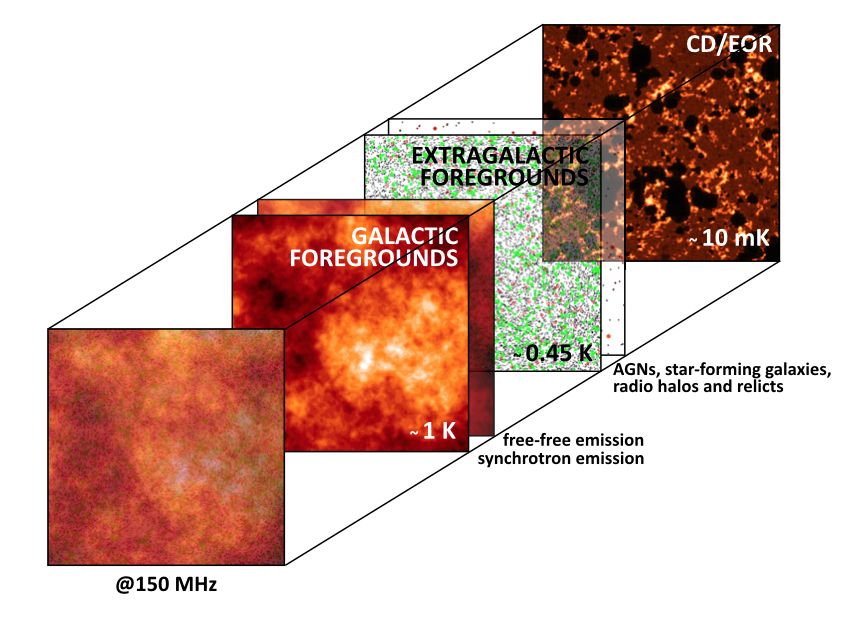
\includegraphics[width=0.95\textwidth]{Chapman_Jelic/Images/fgcube.png}
    \caption{An illustration of different foreground components in the redshifted 21~cm experiments. The images are based on Jeli\'c simulations of the foregrounds \cite{jelic10, jelic08} and 21cmFAST simulations \cite{mesinger11}.}
    \label{fig:fgcube}
\end{figure}

The first overview of the foregrounds was outlined by \cite{shaver99}. Since then various authors have studied the foregrounds in the context of the cosmological 21~cm measurements \cite{bowman09, cooray04, deoliveiracosta08, dimatteo04, dimatteo02, jelic08, jelic10, liu12, oh03, petrovic11, spinelli18, wang06} (see also references in Sec.~\ref{sec:fgmit}).  
At the beginning these studies were mainly based on simulations shaped by extrapolated statistical properties of the foregrounds from the higher radio frequencies. The most comprehensive 
simulation of the foregrounds was carried by \cite{jelic08}.  This simulation has been used extensively in development of the robust foreground mitigation techniques for the LOFAR-EoR project \cite{Chapman2013MNRAS.429..165C, Chapman2012MNRAS.423.2518C, ghosh18,  Harker2010MNRAS.405.2492H, Harker2009MNRAS.397.1138H, Harker2009MNRAS.393.1449H, jelic08, mertens18} and more recently for the SKA CD/EoR project \cite{Chapman2015aska.confE...5C, Chapman2016MNRAS.458.2928C}. In addition to the dedicated foreground simulations, there are also more complex simulations of both Galactic and extragalactic emission, tailored for studies of the interstellar medium and magnetic fields in the Milky Way \cite{haverkorn19, sun09, waelkens09} or of different populations of the radio sources at low-radio frequencies \cite{bonaldi19, wilman10, wilman08}, that can be used as the foreground template in the cosmological 21~cm studies as well.

In parallel to the studies based on simulations, there were also a few dedicated observations taken with the WSRT \cite{bernardi09, bernardi10} and the GMRT \cite{pen09} radio telescopes to constrain the foregrounds at low-radio frequency. However, only once the new low-frequency instruments came online (e.g. EDGES, LOFAR, MWA and PAPER) our knowledge of the foregrounds started to grow extensively. In the following sections a more comprehensive overview of the foregrounds is given both in total intensity and polarization. 

\subsection{Galactic foregrounds in total intensity}
Galactic diffuse synchrotron emission is a dominant foreground component from a few tens of MHz to a few tens of GHz. It is non-thermal in its nature, produced mostly by the relativistic cosmic-ray electrons and to some extent positrons that spiral around the interstellar magnetic field lines and emit radiation.  Above a few tens of GHz free--free emission from diffuse ionized gas and thermal dust emission start to dominate over the synchrotron emission (see Fig.~\ref{fig:galcomp}). 

\begin{figure}[!t]
\centering
    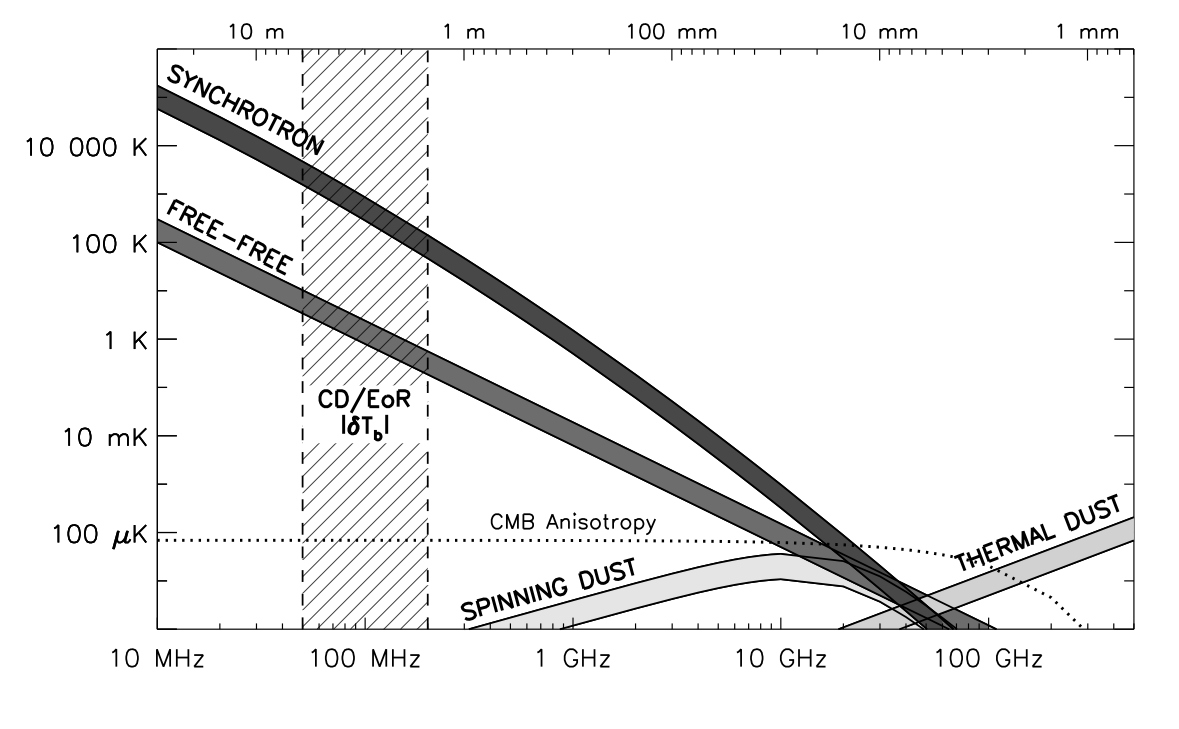
\includegraphics[width=.95\textwidth]{Chapman_Jelic/Images/galcomp.png}
    \caption{The main Galactic diffuse foreground components given as a function of frequency in the total intensity: (i) synchrotron emission from cosmic-ray electrons; (ii) free-free emission from diffuse ionized gas; and (iii) thermal dust emission. There is also a forth component associated with small rapidly spinning dust grains. Synchrotron emission dominates at frequencies below $\sim 10$ GHz, while thermal dust emission dominates at frequencies above $\sim 100$ GHz. Over the whole frequency range of the CD/EoR experiments, Galactic synchrotron emission is 3 -- 4 orders of magnitude stronger in total power (illustrated by the dark grey area) and 2 -- 3 orders of magnitude stronger in fluctuations than the cosmological 21~cm signal ($|\delta T_b|$). In the CMB experiments, on the contrary, there is a sweetspot around $~70$ GHz where the CMB anisotropies are relatively bright compared to the Galactic foreground emission.}
    \label{fig:galcomp}
\end{figure}

For a fairly complete theory of the synchrotron emission  please refer to e.g.~\cite{pacholczyk70,  rybicki86}, while here we outline the basics. The radiated synchrotron power emitted by a single electron is proportional to the square of the electron's relativistic kinetic energy, the magnetic energy density, and the pitch angle between the electron velocity and the magnetic field.  The angular distribution of the radiation is given by the Larmor dipole pattern in the electron's frame, but in the observer's frame is beamed sharply in the direction of motion. 

As the electron spirals around the magnetic field, it is in effect accelerating and emitting radiation over a range of frequencies. Its synchrotron spectrum has a logarithmic slope of 1/3 at low-frequencies, a broad peak near the critical frequency $\nu_c$, and sharp fall off at higher frequencies. The critical frequency is directly proportional to the square of the electron energy and the strength of the perpendicular component of the magnetic field. The longer the electron travels, the more energy it loses, the narrower spiral it makes, and the critical frequency is smaller. 

In the case of the Milky Way we need to take into consideration an ensemble of the cosmic-ray electrons, mainly originating from supernovae located close to the Galactic plane and then diffusing outwards. Given a typical magnetic field strength of a few $\mu$G, the cosmic-ray electrons with energies between 0.5 to 20 GeV account for the observed synchrotron radiation from tens of MHz to hundreds of GHz. Their energy distribution can be approximated with a power law with slope $\delta$:
\begin{equation}\label{eq:ncr}
n_{CR}(E)dE\propto E^{-\delta}dE,
\end{equation}
where $n_{CR}(E)dE$ is the number of cosmic-ray electrons per unit volume with energies between $E$ and $E+dE$. A distribution of their pitch angles is assumed further to be almost random and isotropic due to relatively long timescales (up to several millions of years) over which they lose their relativistic energies and due to repeatedly scattering that occurs in their environments. 

The observed synchrotron spectrum is then given by summing the emission spectra of individual electrons, which are smeared out in the observed spectrum by broad power law energy distribution of the comic-ray electrons. Thus, the synchrotron intensity at frequency $\nu$ depends only on $n_{CR}$ and $\delta$ from Eq.~\ref{eq:ncr} and on the strength of the magnetic field component perpendicular to the line-of-sight $B_\perp$:
\begin{equation}\label{eq:Isyn}
I_{\nu}\propto n_{CR}B_\perp^{(\delta+1)/2}\nu^{(1-\delta)/2}.
\end{equation}
The observed $I_{\nu}$ can be also described as a featureless power law in regards to the observed intensity $I_0$ at a reference frequency $\nu_0$:
\begin{equation}
I_{\nu}=I_0\left( \frac{\nu}{\nu_0} \right)^{-\alpha},
\end{equation}
where observed spectral index $\alpha$ is directly connected to the cosmic-ray  index $\delta$ as $\alpha=(\delta-1)/2$. Moreover,  the observed intensity is commonly expressed in terms of the brightness temperature $T_{b}(\nu)\sim\nu^{-\beta}$, using the Rayleigh-Jeans law which holds at radio frequencies. In this case the observed spectral index is $\beta=2+\alpha=2+(\delta-1)/2$. 

The comic-ray energy slope is estimated to  $-3.0<-\delta<-2.5$ at GeV energies \cite{lawson87, orlando13, strong11}. This corresponds to the synchrotron spectral index of $-1<-\alpha<-0.8$ or $-3<-\beta<-2.8$ observed at GHz frequencies \cite{platania98, reich88}.  At MHz frequencies the synchrotron spectrum is flatter \cite{guzman11, rogers08}. Typical values at mid and high Galactic latitudes are $-2.59 < -\beta < -2.54$ between 50 and 100 MHz \cite{mozdzen19} and $-2.62 < -\beta < -2.60$  between 90 and 190 MHz \cite{mozdzen17}, as measured by the EDGES instrument.  

A difference in the spectral index at MHz and GHz frequencies is due to ageing of the cosmic-ray energy spectrum. As the cosmic-ray electrons propagate trough the interstellar medium, they loose their energies by a number of energy loss mechanisms \cite{longair11} that involve interactions with matter, with magnetic fields and with radiation. This then depletes the population of relativistic electrons and changes their original energy (injection) spectra. For example, the energy loss trough synchrotron radiation is larger for cosmic-ray electrons with higher energies ($\sim E_{CR}^2$). The critical frequency is also proportional to $\sim E_{CR}^2$, so over time, the cosmic-ray spectra becomes steeper together with the synchrotron spectra at higher frequencies.  In a similar way, as the cosmic-ray electrons diffuse away from the Galactic plane, the ageing effect also makes a steepening of the synchrotron spectrum at higher Galactic latitudes \cite{strong07}.

Besides the spectral index variations across the sky, brightness temperature variations of the Galactic diffuse synchrotron emission reflect spatial fluctuations of the comic-ray electron density and magnetic field strength in the interstellar medium. Synchrotron emission is hence the brightest along the Galactic plane, which has the largest concentration of supernovae, a major source of the cosmic-ray particles, while the darkest parts are within the halo. This can be seen in Landecker all-sky map obtained at 150~MHz (see Fig.~\ref{fig:GDSE}, \cite{landecker70}), where typical high latitude brightness is between 150 K and 250 K. Given the low resolution of this map ($\sim5^\circ$), Haslam map at 408~MHz (see Fig.~\ref{fig:GDSE}, \cite{haslam82, haslam81, remazeilles15}) is more commonly used as a template for emission at low radio frequencies. 

\begin{figure}[!t]
\centering
    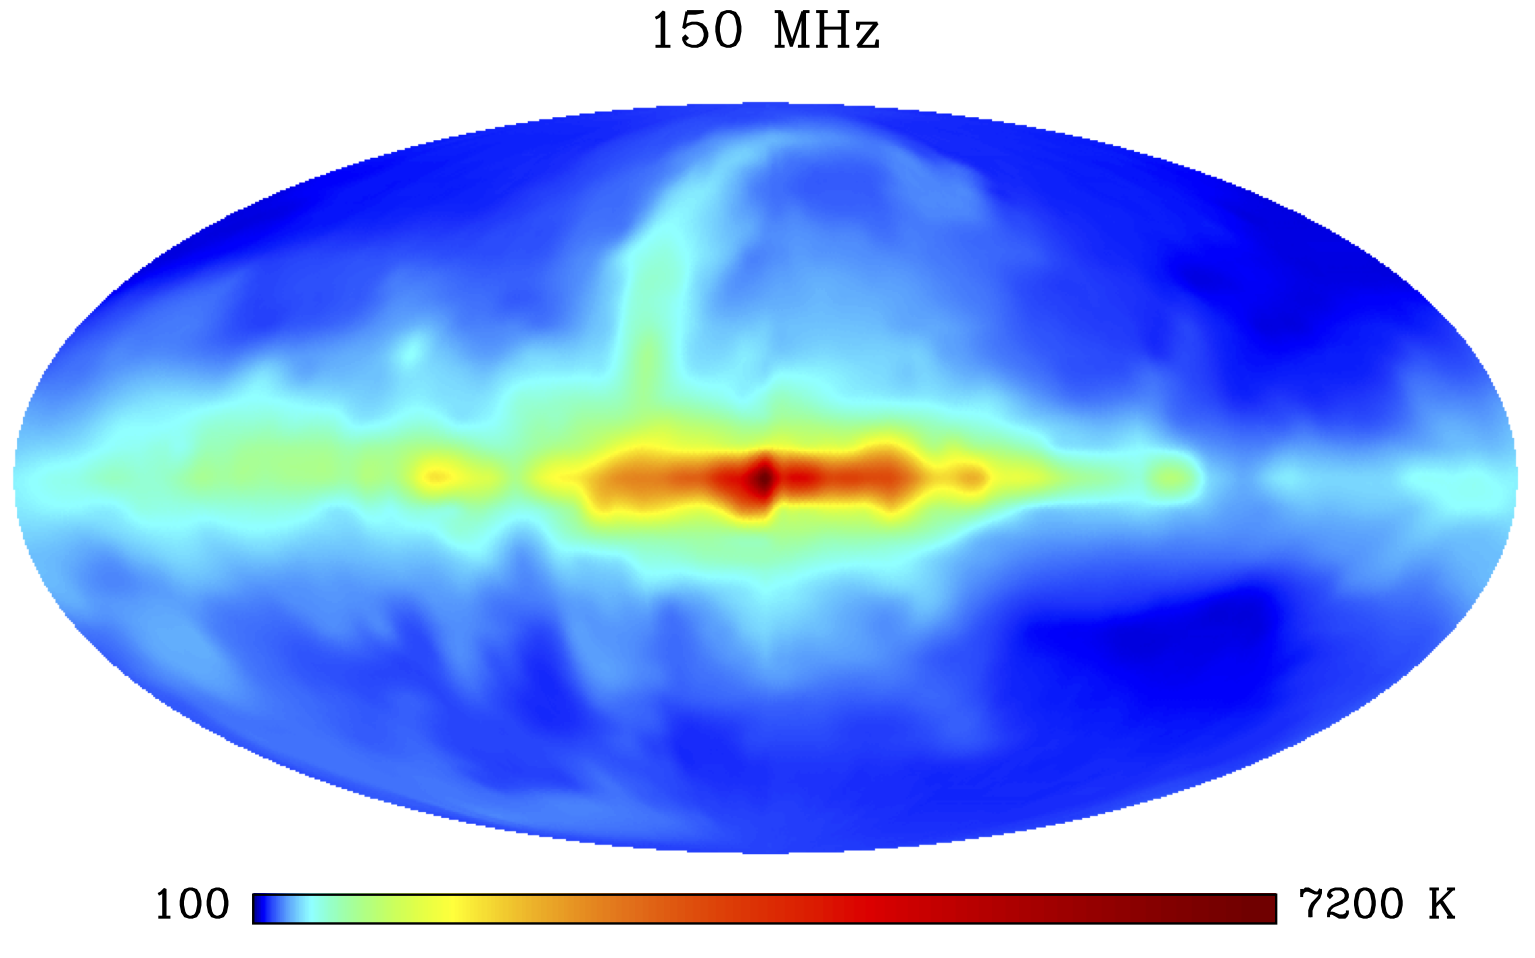
\includegraphics[width=0.475\textwidth]{Chapman_Jelic/Images/landecker.png}
    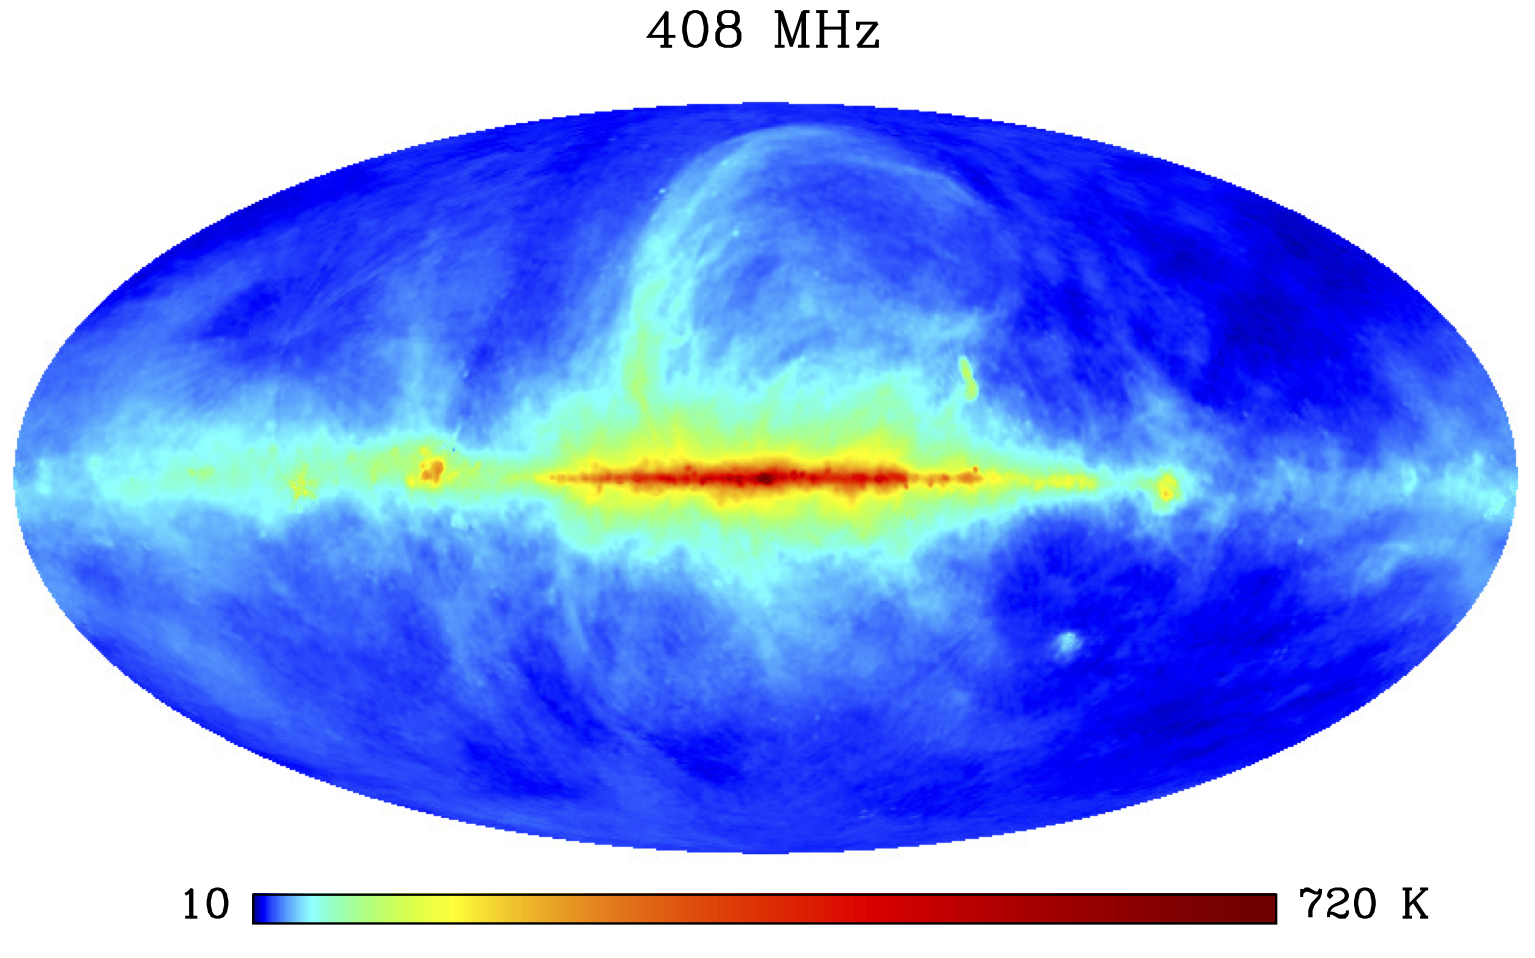
\includegraphics[width=0.475\textwidth]{Chapman_Jelic/Images/haslam.png}
    \caption{All sky maps of Galactic radio emission at 150 MHz \cite{landecker70} and 408 MHz \cite{haslam82, haslam81, remazeilles15}. \textit{This data is available on the Legacy Archive for Microwave Background Data Analysis (LAMBDA, https://lambda.gsfc.nasa.gov), a service of the Astrophysics Science Division at the NASA Goddard Space Flight Center.}}
    \label{fig:GDSE} 
\end{figure}

A number of recent dedicated observations additionally constrained Galactic synchrotron emission in selected areas at high Galactic latitudes. The WSRT observations at 150 MHz show an excess of power attributed to the diffuse synchrotron with an rms of 3 -- 5~K on scales greater than 30~arcmin (observations of the fields around 3C 196 and the North Celestial Pole,  \cite{bernardi10}). The LOFAR observation of the North Celestial Pole \cite{patil17} also clearly shows diffuse emission on scales larger than a degree, while slightly higher levels are found on scales greater than 54~arcmin in the MWA observations at 154~MHz of the fields near the South Galactic Pole \cite{lenc16}.

\subsection{Extragalactic foregrounds in total intensity}
Extragalactic radio sources are of composite nature.  They consist mainly of the active galactic nuclei (AGNs) or the star-forming galaxies (SFGs). 

Radio (synchrotron) emission in the AGNs, so called radio--loud AGNs, is related to the accretion of matter by a supermassive black hole at the centre of its host galaxy, typically an elliptical galaxy.  This produces narrow  jets in a direction perpendicular to the plane of the accretion. The jets can be as large as a few to ten times the size 
of the host galaxy and many of them have diffuse endings, so called radio lobes. Observed morphology of radio loud AGNs varies and can be classified in different ways. For example, we can classified them based on their radio luminosity and brightness of their components (nucleus, jets and lobes) \cite{fanaroff74}. In this case, the FR-I type galaxies  have lower radio powers with an edge darkened morphology, while the FR-II type galaxies have higher radio powers with an edge brightened morphology.

Radio emission in the SFGs is produced like in the Milky Way by synchrotron radiation from supernovae related relativistic electrons and by free-free emission from H{\sc ii} regions. Observed radio emission of these galaxies is usually also tightly connected, although still not well understood why, to the observed infrared luminosity measuring the star-formation rate (e.g.\cite{condon92, helou85, jarvis10}), hence the name SFGs. 

At low--radio frequencies different populations of radio galaxies are still poorly constrained, especially at the faint end of their distribution. There is a low-frequency extragalactic catalogue obtained with the MWA radio telescope in the south (GLEAM \cite{hurleywalker17}) and the ongoing LOFAR Two-metre Sky Survey (LoTTs \cite{shimwell17, shimwell19}) in the north. Until we get deeper with these surveys we need to rely on the data obtained at higher radio frequencies.

Normalised differential source counts for different populations of radio sources at 1.4 GHz is given in Fig.~\ref{fig:extragal}. Thanks to the recent very deep surveys (e.g. COSMOS, \cite{bondi08, novak18, smolcic17b, smolcic17a, smolcic17c} the extragalactic radio sources are constrained well up to the flux densities of $500~{\rm \mu Jy}$. The population of the SFGs dominate at $\mu{\rm Jy}$ levels, while the population of the radio-loud AGNs dominates at flux densities $\geq1~{{\rm mJy}}$ (for a review see \cite{prandoniIAUS333} and references therein). There is also a third population of the sources detected below $\sim100~{\rm \mu Jy}$, commonly referred to as radio-quiet AGNs. These sources do not have large scale radio jets and lobes like radio-loud AGNs. They are probably SFGs hosting also an active nucleus that contributes to the radio emission \cite{ceraj18, delvecchio17}. 

\begin{figure}[!t]
   \centering
    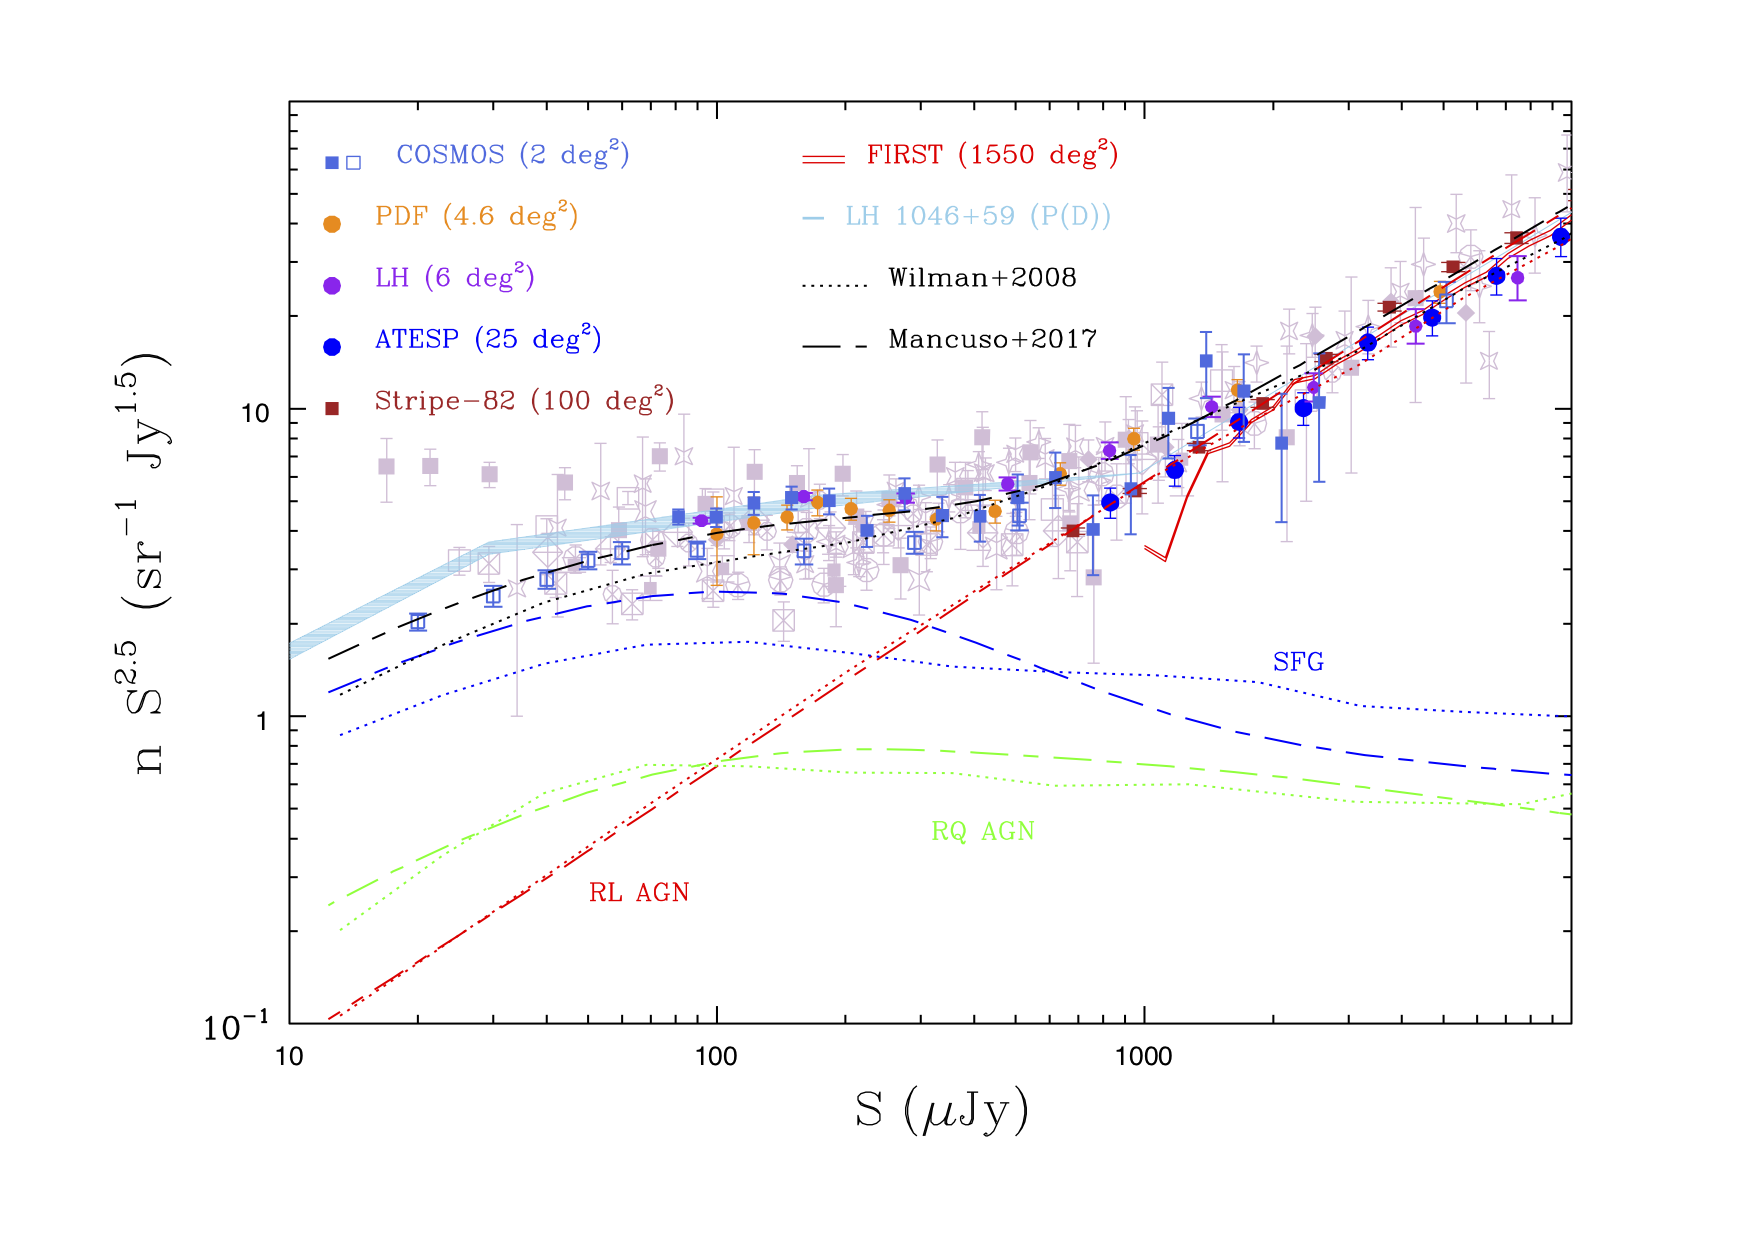
\includegraphics[width=0.95\textwidth]{Chapman_Jelic/Images/extragal.png}
    \caption{Normalized 1.4 GHz differential source counts. for different radio source populations: radio-quite (RQ) AGN, radio-loud (RL) AGN and star-forming galaxies (SFG). The dotted and dashed lines represent predicted counts from different model  \cite{mancuso17,wilman08,wilman10}. Different colours indicate different populations: radio-quite (RQ) AGN, radio-loud (RL) AGN and star-forming galaxies (SFG), while their sum is given in black. Coloured symbols show the counts from a number of large-scale surveys: COSMOS field \cite{bondi08, smolcic17b}; Phoenix Deep Field (PDF, \cite{hopkins03}); the Lockman Hole (LH, \cite{prandoni18}); the ATESP survey \cite{prandoni01}, the Stripe-82 region \cite{heywood16}; and the FIRST survey \cite{white97}. \textit{Reproduced from Prandoni 2018, Proceedings of the International Astronomical Union, IAUS 333:175--182}. }
    \label{fig:extragal}
\end{figure}

In addition to the radio source counts we also need to have a good knowledge of their distribution in the sky (clustering properties) and of their radio spectra. Neglecting source clustering may result in underestimating the angular foreground power which can potentially lead to a false detection of the cosmological 21 cm signal \cite{murray17,murray18}, while if the radio spectra is not smooth the foreground removal will be much more demanding.

The radio spectra of the radio galaxies can be described with the power-law function with a spectral index of  $\alpha\sim-0.7/-0.8$, due to the synchrotron nature of the emission.  Nevertheless, there are process that can change the shape of the spectra (free-free absorption, synchrotron self-absorption, spectral ageing, etc.) and make it complicated. Recent  LOFAR observations of the Bo\"otes field \cite{calistrorivera17} showed significant differences in the spectral curvature between SFG and AGN populations. The radio spectra of SFGs show a weak but statistically significant flattening, while the radio spectra of the AGNs is becoming steeper towards  the lower frequencies. Therefore, different power-law slopes should be assumed for AGNs and SFGs, when modelling the radio sky at frequencies relevant for the cosmological 21 experiments.

\subsection{Polarized foregrounds}\label{sec:polarfg}
Galactic synchrotron emission is partially linearly polarized. Its polarized intensity $PI_\nu$ depends on a cosmic-ray electron density $n_{CR}$, a slope of the cosmic-ray energy spectrum $\delta$, and a strength of the magnetic field component perpendicular to the line-of-sight $B_\perp$, in the same way as defined by Eq.~\ref{eq:Isyn} in total intensity. The only difference is the amount of emission, defined by the degree of polarization \cite{rybicki86}:
\begin{equation}
\Pi=\frac{\delta+1}{\delta+7/3}.
\end{equation}
For $\delta=2.2$, which is consistent with the observed synchrotron spectral index of $-\beta=-2.6$ at 150 MHz \cite{mozdzen17}, we get $\Pi=0.7$. At low radio frequencies  (100--200~MHz) about $70\%$ of Galactic synchrotron emission is intrinsically polarized, while in fact we observe only a few percent \cite{bernardi13, jelic14, jelic15, lenc17, lenc16, vaneck19, vaneck17}. To understand why we observe such a small percentage of polarized emission, we need to take a closer look at Faraday rotation and associated depolarization that occurs. 

As a linearly-polarized wave, with a wavelength $\lambda$, propagates through a magnetised plasma its polarization angle $\theta$ is Faraday rotated by:
\begin{equation}\label{eq:FR}
\frac{\Delta \theta}{\rm [rad]}= \frac{\lambda^2}{\rm [m^2]}\frac{\Phi}{\rm [rad~m^{-2}]}=  \frac{\lambda^2}{\rm [m^2]}\left(0.81\int \frac{n_e}{\rm [cm^{-3}]} \frac{B_{||}}{\rm [\mu G]} \frac{dl}{\rm [pc]}\right),
\end{equation}
where $\Phi$ is Faraday depth, $n_e$ is a density of the thermal electrons, $B_{||}$ is a strength of the magnetic field component parallel to the line-of-sight. The integral is taken over the entire path-length $l$, from the source to the observer.  The Faraday depth is positive when $B_{||}$ points towards the observer, while it is negative when $B_{||}$ points away.

In the Milky Way, where distributions of thermal and comic-ray electrons are perplexed throughout the entire volume, differential Faraday rotation will occur and will depolarize the observed synchrotron emission \cite{sokoloff98}.  As Faraday rotation is proportional to $\lambda^2$, depolarization at low radio frequencies will be significant. 
Nevertheless, small amounts of polarized emission that can still be observed carry valuable information about the physical properties of the intervening magnetised plasma.

\begin{figure}[!t]
\centering
    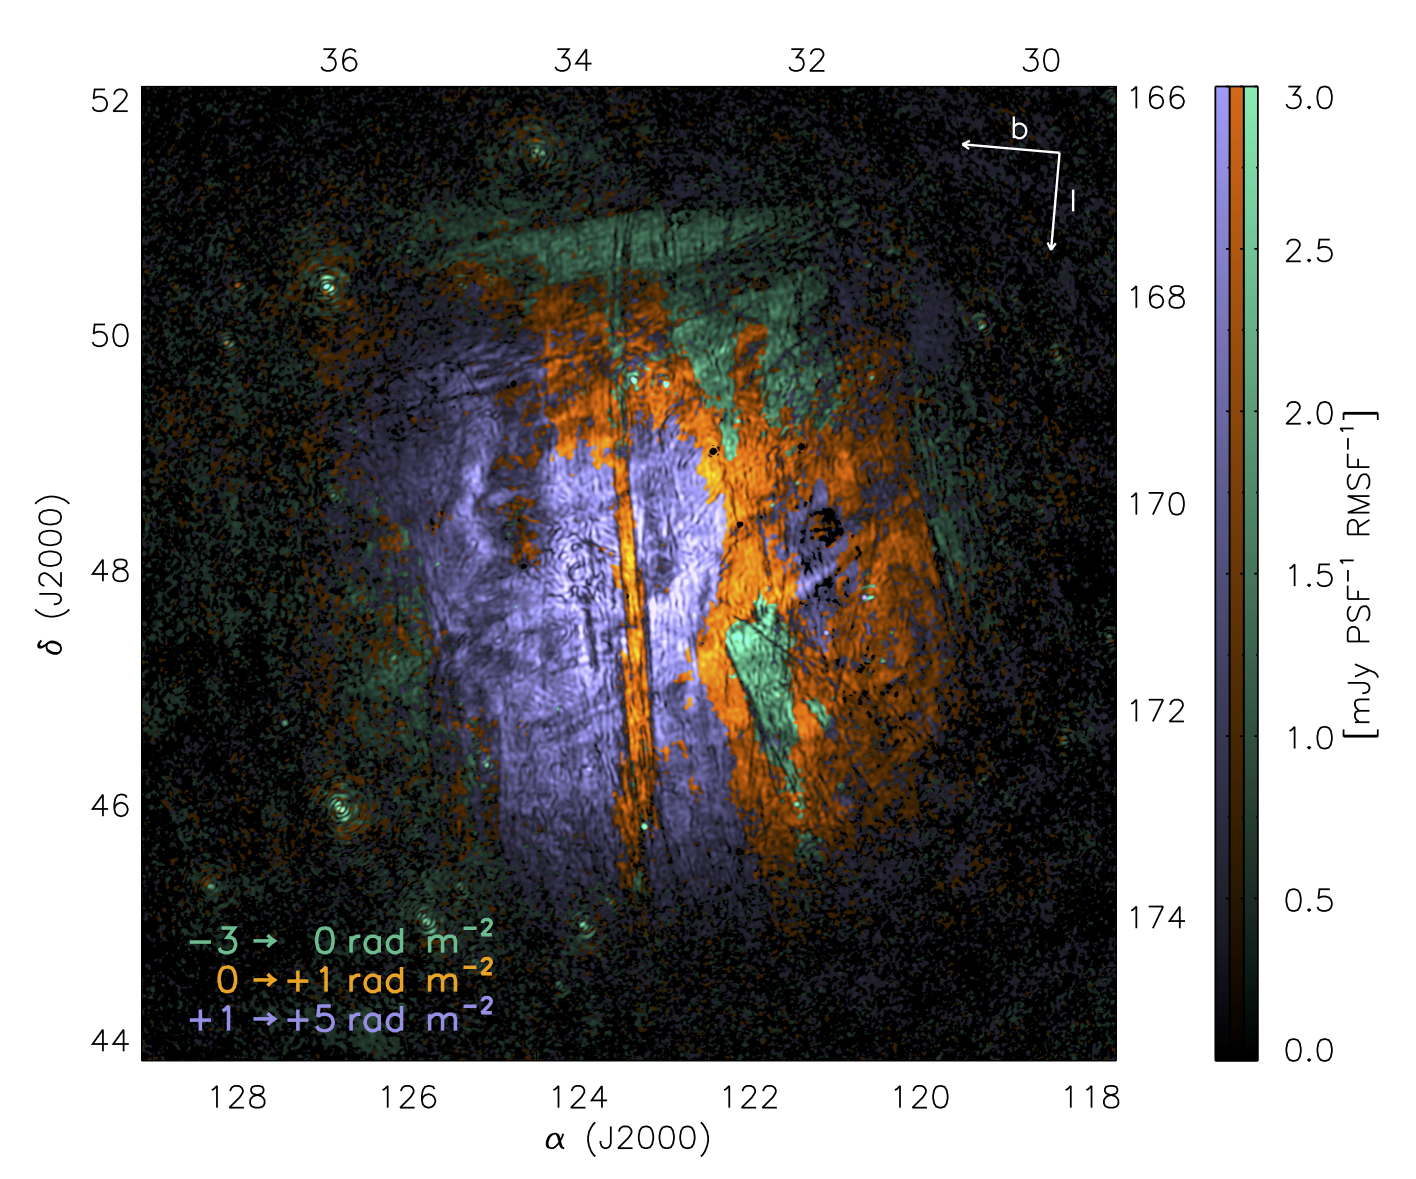
\includegraphics[width=0.475\textwidth]{Chapman_Jelic/Images/3C196.png}
    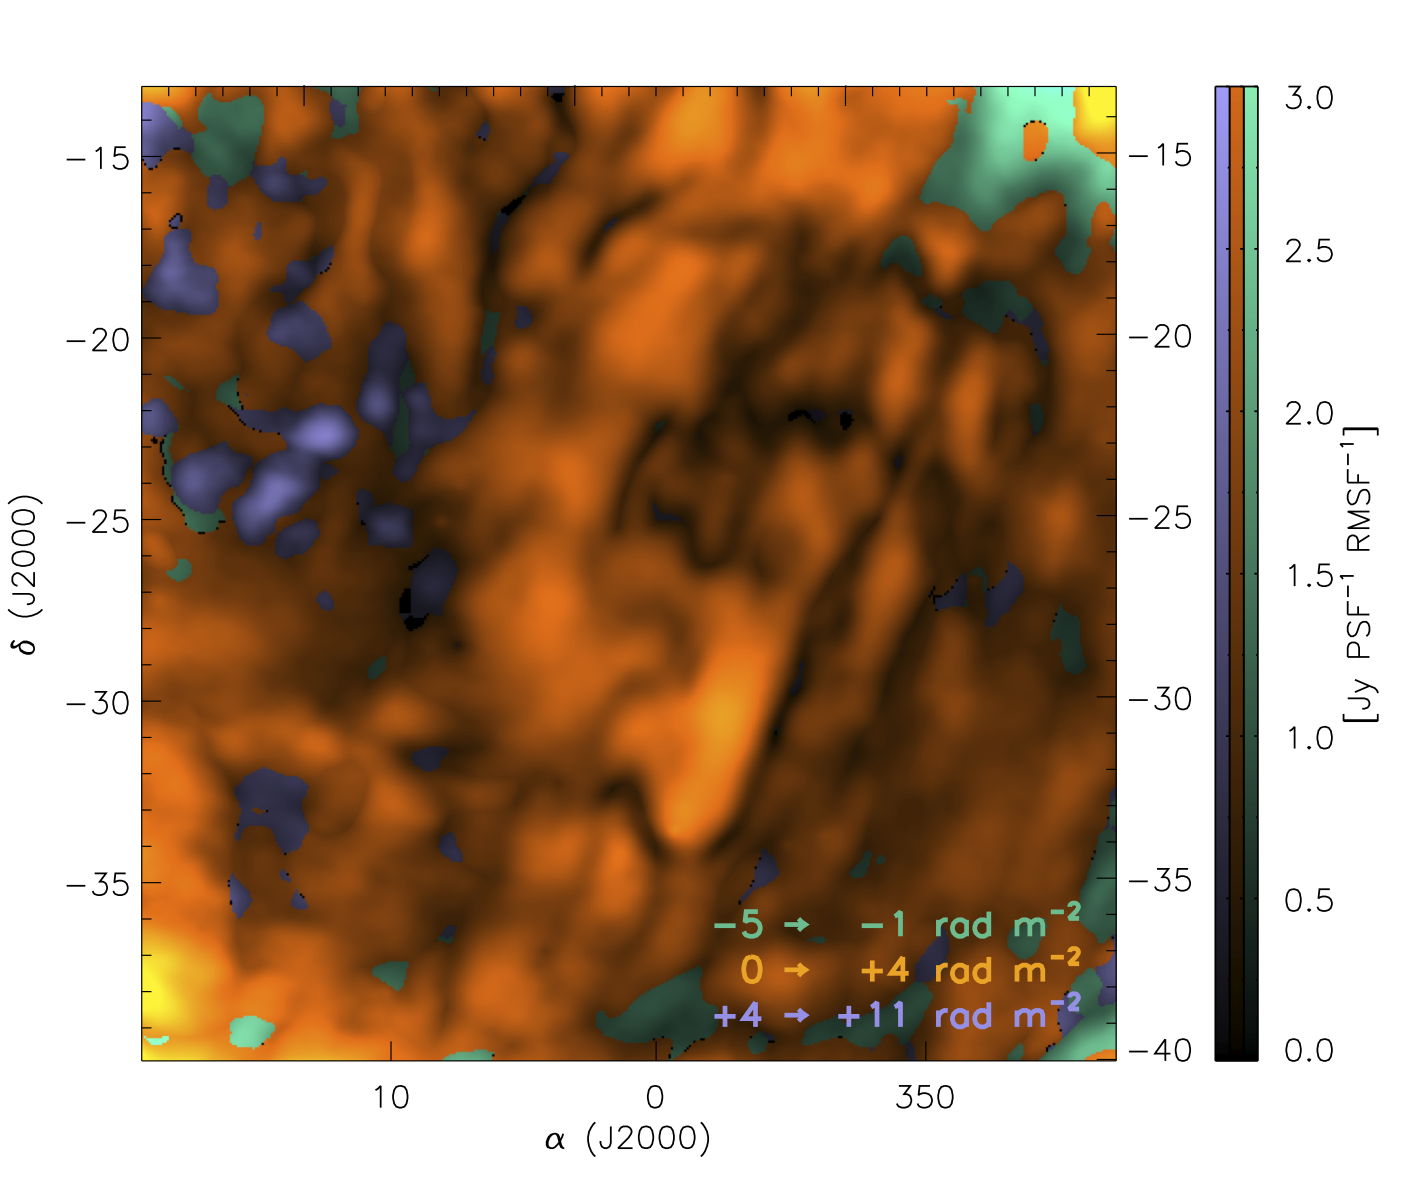
\includegraphics[width=0.475\textwidth]{Chapman_Jelic/Images/lenc.png}
    \caption{Polarized structures discovered at different Faraday depths with LOFAR (an image on the left - \textit{created using the data presented and discussed in Jeli\'c et al. 2015, A\&A, 583:A137, with permission of the authors}) and MWA (an image on the right -  \textit{created using the data presented and discussed in Lenc et al. 2016, ApJ, 830:38, with permission of the authors}) in two fields at high Galactic latitudes.}
    \label{fig:polar}
\end{figure}

First attempts to constrain diffuse polarized emission at 150 MHz were done using the GMRT \cite{pen09} and WSRT observations \cite{bernardi09, bernardi10}.  However, the full richness and complexity of polarized emission at low-radio frequencies was not revealed until LOFAR and MWA came online.  Observations with these instruments discovered astonishing morphology of polarized Galactic synchrotron emission of a few Kelvin in brightness (see Fig.~\ref{fig:polar} and \cite{bernardi13, iacobelli13b, jelic14, jelic15, lenc16, lenc17, vaneck19, vaneck17}). The discovered structures were unraveled by Rotation Measure (RM) synthesis \cite{brentjens05}. This is a technique in radio polarimetry that disentangles the observed wavelength-dependent polarization into a Faraday spectrum, i.e., the distribution of polarized emission as a function of Faraday depth. This allow us then to preform, so called, Faraday tomography, a study of the intervening magnetised plasma as a function of Faraday depth.

Given a wide frequency coverage and a high spectral resolution available in the low-frequency instruments Faraday tomography is preformed at an exquisite sensitivity and resolution in Faraday depth of $\sim1~{\rm rad~m^{-2}}$, an order of magnitude higher than at 350 MHz. This allow us to map small column densities of magnetised plasma that are, in most cases, not possible to detect at higher radio frequencies. Interestingly, most of the observed structures at low-radio frequencies appear at Faraday depths $\Phi\leq15~{\rm rad~m^{-2}}$ and they are not correlated with structures in total intensity. This result will be relevant in later discussion of the polarization leakage in the cosmological 21~cm experiments (see Sec.~\ref{sec:leakage}).

Extragalactic polarized sources are not a big concern for the cosmological 21~cm experiments due to their sparsity in the sky. In the MWA 32-element prototype survey of 2400 deg$^2$ of the southern sky at 189 MHz only one polarized source was found \cite{bernardi13}. In a preliminary data release of the LOFAR Two-meter Sky Survey of the HETDEX field, covering an area of 570 square degrees, 92 polarized radio sources where found \cite{vaneck18}. This gives a lower limit to the polarized source surface density at 150 MHz of only 1 source per 6.2 square degrees. Somewhat higher value, 1 source per 2 degrees, was found based on LOFAR observations of three 16 deg$^2$ fields \cite{jelic15, mulcahy14, vaneck18}.

\subsection{Radio Frequency Interference}
Terrestrially, radio frequency interference (RFI) from any human-made sources of radio transmission, such as wind turbines, leads to the necessary excision of frequency channels using a flagging technique (e.g. \cite{Offringa2012, Prasad2012ExA....33..157P}. The number of channels excised is significant, around 1$\%$ of channels of data for MWA and LOFAR \cite{Offringa2019MNRAS.484.2866O,Offringa2015PASA...32....8O}. Without careful mitigation in the calibration, imaging and diffuse foreground removal stages, RFI excision can result in an excess power that scales with the number of excised channels and does not integrate down with time, significantly dominating over the cosmological 21-cm signal by 1-2 magnitudes \cite{Offringa2019MNRAS.484.2866O}.
 
\section{Foreground Mitigation}\label{sec:fgmit}

The 21-cm signal emitted by high-redshift neutral hydrogen provides a window into the Epoch of Reionization (EoR), but it is a window that is obscured by layers of foregrounds. Extra-terrestrially, there exist a multitude of foregrounds which dominate all frequencies of observation and so more subtle methods than excision are required. This part of the chapter discusses the development and current use of Galactic and extragalactic foreground mitigation methods in Epoch of Reionization 21-cm experiments.

\subsection{Foreground Mitigation in the Data Analysis Pipeline}
\subsubsection{Bright Source Removal}
The first stage of foreground removal involves mitigating the effect of the very brightest sources on the sky: the point sources and extended sources. Bright source removal often comes under the umbrella of calibration as opposed to foreground mitigation however we will briefly summarize the process here. For example, the MWA real-time system (RTS) \cite{Mitchell2008ISTSP...2..707M} carries out sequential bright source `peeling' on the visibilities, tracking a few hundred of the brightest sources and comparing to a sky model constructed from existing catalogues and MWA observations \cite{Carroll2016MNRAS.461.4151C}. The gains are calibrated on the strongest source, before that source is peeled (subtracted) from the data, and the next strongest source is used to refine the calibration, and so on until it is deemed that enough bright sources have been removed, usually a few hundred to a thousand at most. The other MWA calibration pipeline, Fast Holographic Deconvolution (FHD) \cite{Sullivan2012ApJ...759...17S}, uses the MWA extragalactic catalogue GLEAM \cite{hurleywalker17} to calibrate gains, modelling all sources out to 1$\%$ beam level in the primary lobe, amounting to approximately 50000 sources \cite{Barry2019arXiv190102980B} and then removing a smaller population of them from the data. Similarly, LOFAR has built up a sky model over several years using the highest resolution LOFAR images and subtracts the sources in visibility space also \cite{Yata2015MNRAS.449.4506Y,Yata2013AA...550A.136Y}. As of 2017, the LOFAR EoR sky model contained around 20,800 unpolarized sources. 

\subsubsection{The EoR Window}
\label{sec:wedge}

It has previously been traditional when discussing diffuse foreground mitigation to assume that the previous stage of bright source subtraction has already been implemented perfectly. This is no longer seen to be a valid or safe assumption, as the chromaticity of the instrument, calibration errors and incorrect source subtraction lead to significant bias in the EoR signal for all current and planned experiments (e.g. \cite{ EW2017MNRAS.470.1849E,Procopio2017PASA...34...33P,Barry2016MNRAS.461.3135B,Patil2016MNRAS.463.4317P,Datta2010ApJ...724..526D,Liu2009MNRAS.394.1575L}, including redundant arrays \cite{Byrne2019ApJ...875...70B}. 

\begin{figure}
\begin{center}
    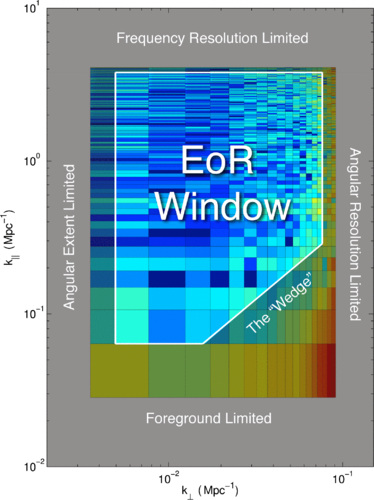
\includegraphics[width=0.5\textwidth]{Chapman_Jelic/Images/medium.png}
\end{center}
    \caption{A schematic of the `EoR Window' in the cylindrical $k_{\parallel}$,$k_{\perp}$ Fourier plane, taken from Fig.1 of \cite{Dillon2014PhRvD..89b3002D}. In a perfect observation, with zero instrumental effects, the foregrounds would be entirely contained in the well defined horizontal band. In a realistic observation however, the chromaticity of the instrument results in a leakage of power up into the EoR window, into a region called the `wedge'. Aside from these contaminated areas there should be a relatively clean area called the EoR window. \textit{Reproduced from Dillon, Liu, Williams et al. (2014), PhysRevD, 89(2):023002}.} 
    \label{fig:window_liu}
\end{figure}

The spectral differences between the EoR signal and the bias introduced by the foregrounds and instrument lend themselves to a neat separation in $k_\bot-k_\parallel$ space, Fig. \ref{fig:window_liu}. In this formalism, spectrally-smooth foregrounds live in a well-defined area of $k$-space, at the smallest $k_\parallel$ scales, equivalent to the red stripe at the bottom of Fig. \ref{fig:window_liu}, excluding the wedge area. The assumption that the foregrounds would remain smooth and confined in a horizontal area at low $k_\parallel$ even after observation by a radio interferometer drove early foreground removal techniques such as those introduced in Section \ref{sec:poly} but is now known to be an incorrect assumption. The chromaticity of the instrument results in a `mode-mixing' where power is transferred from the angular to the frequency scales, throwing power upwards from the foreground area in the window into the larger $k_\parallel$ scales, with the effect increasing with larger $k_\bot$. This results in a wedge like structure, a structure that has been now extensively discussed and mathematically defined in the literature (e.g. \cite{Jensen2016MNRAS.456...66J,Dillon2014PhRvD..89b3002D,Liu2014PhRvD..90b3019L,Liu2014PhRvD..90b3018L,Hazelton2013ApJ...770..156H,Thyagarajan2013ApJ...776....6T,Pober2013ApJ...768L..36P,Morales2012ApJ...752..137M,Vedantham2012ApJ...745..176V,Trott2012ApJ...757..101T,Parsons2012ApJ...756..165P,Datta2010ApJ...724..526D}. Because the point sources reside on the largest $k_\bot$ scales they, or even their residuals when incorrectly calibrated, can overwhelm the EoR power in the frequency scales (e.g. \cite{Bowman2009ApJ...695..183B} and immediately preceding references).

Now we have defined the problem, namely the overpowering magnitude and potential leakage of foregrounds onto the EoR signal, we can consider how to achieve our aim of making accurate statistical conclusions on the nature of the EoR using the data within this window. To proceed, we can consider two philosophies. The first, \textbf{foreground subtraction}, aims to remove foreground contamination on all scales. The benefit of this is that there are more $k$ scales available for analysis. The drawback of foreground subtraction across all $k$-scales is that any failure in the method will potentially result in a foreground fitting bias across all scales of the window, providing another layer of contamination. One could instead avoid the foregrounds and therefore the need to remove them: \textbf{foreground avoidance}. This philosophy aims to then quantify the foregrounds and wedge such that any analysis occurs within a well-defined window free of contamination. The benefit of this is, as stated, the avoidance of foreground subtraction bias. The drawback is that any analysis is performed on a significantly reduced set of scales which can for example introduce its own bias into the spherically averaged power spectrum \cite{Jensen2016MNRAS.456...66J}. Additional to both philosophies, we can implement \textbf{foreground suppression}, which down-weights scales where the foregrounds or foreground removal residuals are dominant. We will now discuss these approaches in further detail in the context of current EoR experiments.

\subsection{Foreground Avoidance and Suppression}

The Murchison Widefield Array (MWA) has two separate pipelines which differ in their application of foreground mitigation techniques and calibration methods, while mostly employing foreground avoidance. The way in which MWA is optimized for making images allows the option to directly subtract known foregrounds but in this case the direct foreground subtraction is primarily applied to get access to a cleaner EoR window, not to get access to within the wedge, as is the motivation of foreground subtraction in LOFAR.

\begin{figure}
\begin{center}
    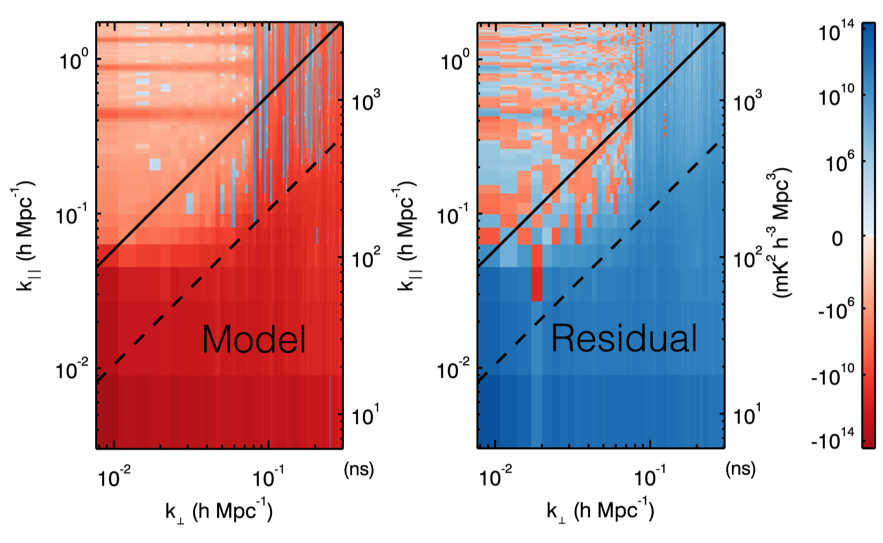
\includegraphics[width=0.9\textwidth]{Chapman_Jelic/Images/apjaa3b64f9_hr.png}
\end{center}
\caption{Left: The difference between the MWA foreground model without diffuse foregrounds (i.e. just point sources) and with diffuse foregrounds. Adding diffuse foregrounds into the model produces leakage far up into the EoR window and instrumental contamination can be seen in the horizontal lines throughout the EoR window. Right: the difference between the power spectrum of the residuals when only the point sources have been subtracted as described above, and the power spectrum of the residuals where the diffuse foregrounds have also been subtracted. There is a clear reduction in foreground residuals all along the wedge and the EoR window is noise-like, suggesting a lack of foreground contamination there. There is a 70$\%$ reduction in residual power of the foregrounds using this method. \textit{Reproduced from Beardsley, Hazelton, Sullivan et al. (2016), ApJ, 833(1):102}.}
    \label{fig:beardsley_fg_sub}
\end{figure}

The FHD \cite{Sullivan2012ApJ...759...17S} and $\epsilon$psilon \cite{Barry2019arXiv190102980B} pipeline builds a sky model of point sources based on a golden set of data, including all sources above a floor limit within the primary beam of the instrument, and those beyond the primary beam if they are above 1$\%$ of the maximum primary beam level. This point source model is used in calibration in a similar way to LOFAR, and contains about 7000 sources as of 2016 \cite{Beardsley2016ApJ...833..102B}. In contrast to the RTS \cite{Mitchell2008ISTSP...2..707M} and CHIPS \cite{Trott2016ApJ...818..139T} pipeline, the FHD-$\epsilon$psilon pipeline also generates a diffuse foreground model by subtracting away the point source model from the observed data, and integrating over frequency to create a diffuse foreground model free of spectral information \cite{Beardsley2016ApJ...833..102B}. They then subtract both the point source model and the diffuse model from the data to minimise the leakage from the wedge into the EoR window. In Fig \ref{fig:beardsley_fg_sub} we see the effect of this foreground subtraction on the EoR window. The left image is the difference between the power spectrum of the MWA foreground model without diffuse foregrounds (i.e. just point sources) and with diffuse foregrounds. The plot shows that the diffuse foregrounds have power far up into the EoR window, due to non-uniform spectral sampling and the effect of windowing the data along frequency during the Fourier Transform. This figure if no other demonstrates the danger of assuming that the observed foreground signal is smooth and contained only at the smallest $k_\parallel$. Further instrumental complications can be seen in the horizontal lines throughout the EoR window, which is contamination due to the periodic frequency sampling function used by MWA \cite{Offringa2016MNRAS.458.1057O}. The right plot of Fig. \ref{fig:beardsley_fg_sub} shows the difference between the power spectrum of the residuals when only the point sources have been subtracted as described above, and the power spectrum of the residuals where the diffuse foregrounds have also been subtracted. There is a clear reduction in foreground residuals all along the wedge and the noise-like characteristic of the EoR window suggests a lack of foreground contamination there. \cite{Beardsley2016ApJ...833..102B} report a 70$\%$ reduction in residual power of the foregrounds using this method.

The black lines in Fig. \ref{fig:masks} show the area of the EoR window used in the FHD-$\epsilon$psilon pipeline, with the masks ensuring the avoidance of the horizontal contamination lines and the wedge.

\begin{figure}
\begin{center}
    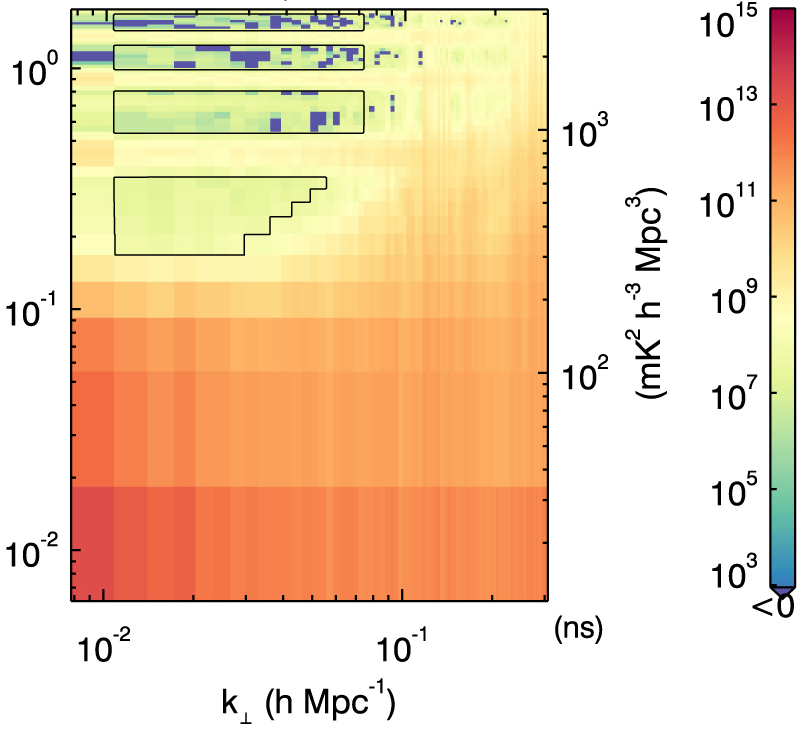
\includegraphics[width=0.9\textwidth]{Chapman_Jelic/Images/apjaa3b64f13_hr.jpg}
\end{center}
    \caption{An example 2D cylindrical power spectrum of the first season MWA data after foreground mitigation. The data used for the upper limits can be seen bounded by black lines. The amount of data available for a power spectrum analysis has been severely reduced by the presence of foregrounds and instrumental contamination but the data within the bounded regions displays noise-like behaviour indicative of successful foreground mitigation. \textit{Reproduced from Beardsley, Hazelton, Sullivan et al. (2016), ApJ, 833(1):102}.}
    \label{fig:masks}
\end{figure}

The RTS-CHIPS pipeline subtracts significantly fewer sources, a few hundred to a thousand at most, and does so in visibility space. There is no diffuse foreground model in the subtraction stage and instead CHIPS down-weight modes with residual point source power. There is also the option of diffuse foreground weighting based on a simple foreground model where the covariances are known, though in practice this diffuse down-weighting is not currently utilised.

\subsubsection{Delay Space Filtering}
Delay space filtering is a method of foreground avoidance primarily adopted by the Donald C. Backer Precision Array for Probing the Epoch of Reionization (PAPER) \cite{Parsons2010AJ....139.1468P}. As with most foreground mitigation methods it requires the foregrounds to be reasonably smooth, even after instrumental effects. The wedge is the end-result of an instrument where the frequency-dependence of the instrument's sampling is dependent on the length of the baseline measuring the sky. Delay-space filtering exploits this relation by analyzing the data per baseline, circumventing the conspiracy of instrumental effects on the foregrounds and effectively isolating the foregrounds such that they are easily avoided. Fig. \ref{fig:baselines} demonstrates that for a given baseline measurement the visibility sampled changes with frequency, with a steeper change for longer baselines. This results in the mode-mixing seen in the 2D cylindrical power spectrum and the wedge structure, where we see power thrown up into the EoR window increasingly on the largest $k_\bot$ scales, which are the scales sampled by the longest baselines. Delay space filtering aims to mitigate the mode mixing by performing a Fourier transform along the visibility sampled by a given baseline (a solid line in Fig. \ref{fig:baselines}, and not along the frequency direction (vertical axis of Fig. \ref{fig:baselines}as is usual.

\begin{figure}
\begin{center}
    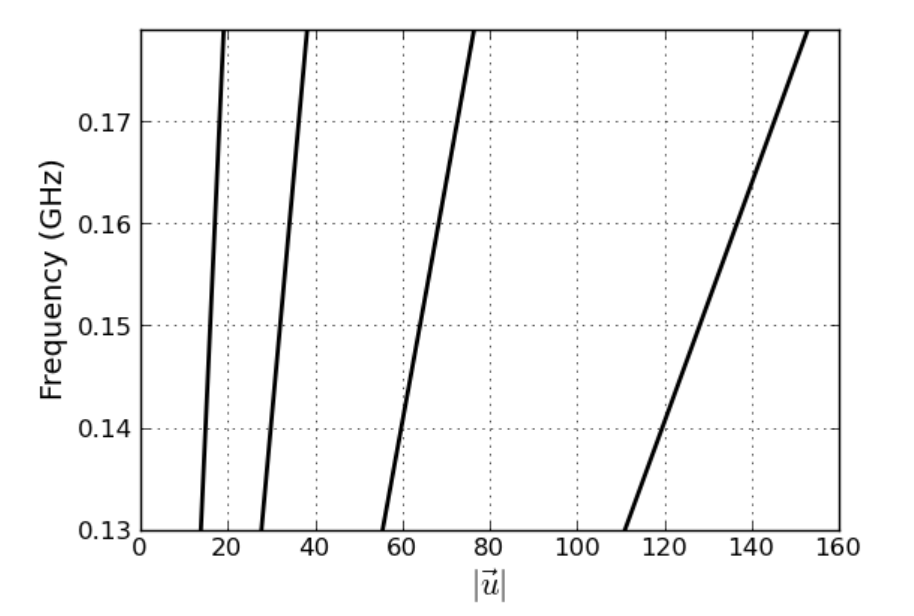
\includegraphics[width=0.5\textwidth]{Chapman_Jelic/Images/baselines.png}
\end{center}
    \caption{This figure demonstrates the frequency dependence of the wavemode sampled by baselines measuring 16, 32, 64, and 128 wavelengths at 150 MHz. For a given baseline measurement, the visibility sampled changes with frequency, with a steeper change for longer baselines. This results in the mode-mixing seen in the 2D cylindrical power spectrum and particularly "the wedge", where we see power thrown up into the EoR window increasingly on the smallest $k_\bot$ scales, which are the scales sampled by the longest baselines. \textit{Reproduced from Parsons, Pober, Aguirre et al. (2012), ApJ, 756(2):165}.}
    \label{fig:baselines}
\end{figure}

A delay transform takes a single time sample of a visibility from one baseline, for all observed frequencies (i.e. one of the solid lines on Fig. \ref{fig:baselines}, and Fourier transforms it to produce the delay spectrum \cite{Parsons2012ApJ...756..165P,Parsons2012ApJ...753...81P,Parsons2009AJ....138..219P}. The delay transform is:

\begin{equation}
    \widetilde{V}_b(\tau) = \int dl \; dm \; d\nu \; A(l,m,\nu)I(l,m,\nu)e^{-2\pi i\nu(\tau_g-\tau))}
\end{equation}

\noindent where $l,m$ have their usual definition relating to angular coordinates on the sky (e.g. \cite{Thompson2001isra.book.....T}). $\tau$ is the time-delay between the signal reaching both antennas and the geometric group delay associated with the projection of baseline $\overrightarrow{b} \equiv (b_x,b_y,b_z) $ in the direction $ \hat{s} \equiv (l,m,\sqrt{1-l^2-m^2})$ is:

\begin{equation}
    \tau_g \equiv \frac{\overrightarrow{b} \cdot \hat{s}}{c} 
\end{equation}

For comparison, the usual equation where the Fourier transform is simply applied along the frequency axis is:

\begin{equation}
    \widetilde{V}(u,v,\eta) = \int dl \; dm \; d\nu \; A(l,m,\nu)I(l,m,\nu)e^{-2\pi i(ul+vm+\eta\nu)}
\end{equation}

\noindent where $\eta$ is the Fourier transform of $\nu$.

The delay transform transforms flat spectra sky emission into delta functions. Because the sky emission is not perfectly smooth, and the instrument adds in its own unsmoothing effects, this delta function is effectively convolved with a kernel, which broadens the delta function in delay space. For the smoother foregrounds, that kernel will be narrow, and confined within the ``horizon limits", the geometric limit in delay space beyond which no flat spectra emission can enter the telescope. Spectrally unsmooth sky emission can enter beyond these horizon limits and emission such as the cosmological signal finds itself with a wide convolving kernel, spreading power well beyond the horizon limit where the foregrounds are theoretically confined. In Fig. \ref{fig:horizon} we see the delay transform at 150 MHz for several spectrally smooth sources and how they remain confined within the horizon limits of the baseline (here 32 metres). In contrast, the delay spectrum of spectrally unsmooth emission, such as the cosmological 21-cm signal, finds itself smeared to high delays. Full mathematical detail can be found in \cite{Parsons2012ApJ...756..165P,Parsons2012ApJ...753...81P} and \cite{Parsons2009AJ....138..219P}.

\begin{figure}
\begin{center}
    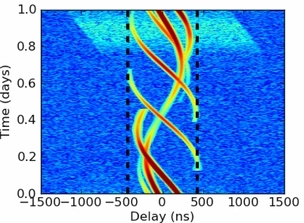
\includegraphics[width=0.5\textwidth]{Chapman_Jelic/Images/horizon.jpg}
\end{center}
    \caption{The delay spectra of several smooth-spectra sources, which remain largely confined within the geometric horizon limits. The broad 21-cm cosmological signal delay spectra in cyan demonstrates that unsmooth spectral signals have a much wider convolving kernal and produce a much wider delay spectra. If analysis is carried out outside of the horizon limits then the foregrounds can be avoided. \textit{Reproduced from Parsons, Pober, Aguirre et al. (2012), ApJ, 756(2):165}.}
    \label{fig:horizon}
\end{figure}

By performing this delay space transform, we are effectively moving into the sidelobes of the 21-cm signal in delay space. The cosmological signal is scattered to high delays whereas the foregrounds are not, allowing the data analysis in that large delay space to be free of foregrounds and foreground removal bias. This method also removes the need for imaging in order to remove the foreground directly, making it suitable for a redundant array with little or no ability to image, but a high sensitivity to the 21-cm power spectrum \cite{Parsons2012ApJ...753...81P}.   

PAPER is a radio interferometer with a highly redundant antenna layout, with multiple baselines of the same length and orientation. Because these multiple baselines all measure the same sky signal, any differences in the signal received would be due to instrumentation, allowing a quick calibration for multiple calibration parameters - `redundant calibration' (e.g. \cite{Ronniy2018AJ....156..285J,Li2018ApJ...863..170L,Dillon2016ApJ...826..181D,Zheng2014MNRAS.445.1084Z,Wieringa1992ExA.....2..203W}). 

PAPER avoided the use of the delay modes dominated by foregrounds and downweighted residual foregrounds using inverse covariance weighting in order to form an upper limit power spectrum measurement \cite{Ali2015ApJ...809...61A}. The latter method of inverse covariance weighting where the covariance is calculated based on the data itself has now been shown to carry the considerable risk of overfitting the EoR data \cite{Cheng2018ApJ...868...26C}. To be clear, despite the retraction of the PAPER-64 results due to power spectrum estimation errors \cite{Ali2018ApJ...863..201A}, the delay space filtering technique remains a promising approach to foreground mitigation.

\subsection{Foreground Subtraction}\label{sec:fgsub}
Foreground subtraction methods all seek to find a model for the observed foregrounds and remove that model from the observed signal, leaving the cosmological signal, instrumental noise and any foreground fitting errors. Foreground removal is usually applied on all scales, meaning that it potentially allows access into the lowest $k_\parallel$ scales where foregrounds traditionally dominate. A caveat of this is that any foreground fitting bias has the potential to affect all scales in the window: foregrounds may remain within the wedge and cosmological signal may be erroneously fitted out within the previously clean EoR window. As an aside, there has been no method so far that can separate out the cosmological 21-cm signal entirely by itself, separate from instrumental noise. Currently when the foregrounds are subtracted or avoided the noise and cosmological signal are still mixed together in what are often termed the `residuals'. The instrumental noise can be obtained from the data for example by the differencing of very fine bandwidth frequency channels, such that both the foregrounds and EoR signal are smooth. The noise power spectrum can then be removed from the residual power spectrum to form the recovered cosmological signal power spectrum. We will now introduce some of the main foreground subtraction techniques.

\subsubsection{Polynomial Fitting and Global Experiments}
\label{sec:poly}

\begin{figure}
\begin{center}
    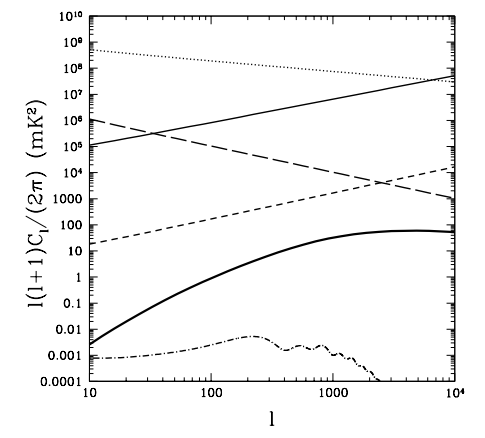
\includegraphics[width=0.4\textwidth]{Chapman_Jelic/Images/santos_spat.png}
    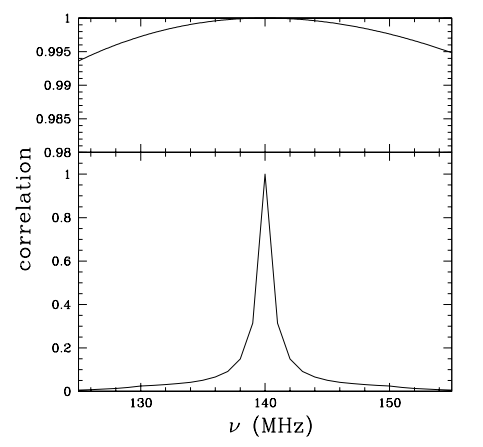
\includegraphics[width=0.4\textwidth]{Chapman_Jelic/Images/santos_freq.png}
\end{center}
    \caption{Left: The 2D power spectrum at 140MHz for the cosmological signal (thick, solid), point sources (thin, solid), Galactic synchrotron (thin, dotted), extra-Galactic free-free (thin, dash), Galactic free-free (thin, long dash) and the CMB (dot-dash). The cosmological signal is dominated by foregrounds at all scales, such that separation based purely on spatial differences in not feasible. Figure taken from Fig. 5 of \cite{Santos2005ApJ...625..575S}. Right: The simulated frequency correlations for the foregrounds (top) and cosmological signal (bottom). This plot shows how the correlation between frequency slices (with the comparison made to a slice at 140 MHz), drops off with increasing frequency separation. The foregrounds are highly frequency coherent, whereas the cosmological signal is significantly less so. \textit{Reproduced from Santos, Cooray and Knox (2005), ApJ, 625(2):575--587}.}
    \label{fig:santos_spatial}
\end{figure}

As we have seen in the first half of this chapter, the astrophysical foregrounds are 3-5 magnitudes brighter than the cosmological 21-cm signal and so, by magnitude alone, appear to be the most ominous obstacle to the first detection. Despite, or perhaps because of, their overwhelming magnitude they are well constrained, following power laws with known indices and evolution. The sheer magnitude of the foregrounds means that purely spatial separation, i.e. separation based on only one frequency slice, is not possible: the 21-cm signal and foregrounds are not statistically different enough when only considering spatial scales (see left-hand panel of Fig. \ref{fig:santos_spatial}) \cite{Santos2005ApJ...625..575S,DiMatteo2004MNRAS.355.1053D,Oh2003MNRAS.346..871O,DiMatteo2002ApJ...564..576D}. While separation based purely on spatial scales is not feasible, the high frequency coherence of the foregrounds compared to both the instrumental noise and cosmological signal provides a way to separate out the two signals (foregrounds and both cosmological signal and noise) (see right-hand panel of Fig. \ref{fig:santos_spatial}). 

\cite{Santos2005ApJ...625..575S} and \cite{Zal2004ApJ...608..622Z} exploited the large cross-correlation of the foregrounds in slices at different frequencies to model and remove the foregrounds noting that the frequency coherence was also a useful tool for separation. Polynomial fitting went on to exploit the frequency coherence of the foregrounds across the bandwidth, removing the foregrounds along the line of sight without using any spatial correlation information (e.g. \cite{Bowman2009ApJ...695..183B,Wang2006ApJ...650..529W,Mcquinn2006ApJ...653..815M}. In this method, the foregrounds are modelled by a polynomial function, for example in log-log space such as:

\begin{equation}
\mathrm{\log I} = a_3 +a_2\log\nu + a_1(\log \nu)^2 + ....
\end{equation}

\noindent where $I$ is the brightness temperature of the data, $\nu$ is the frequency of observation and $a_1,a_2,a_3$ are the coefficients which are to be determined in the fit.

Polynomial fitting is a parametric foreground mitigation method. It uses knowledge from simulated foregrounds to tune the coefficients of the polynomial function (e.g. \cite{jelic08}). There are two areas of concern when using this method. Firstly, the effect of the instrument results in a signal which can differ significantly from the frequency-coherent theoretical foreground model (see Section \ref{sec:wedge}). By incorporating weighting according to the amount of information in a particular $uv$ cell, this could possibly be overcome \cite{Liu2009MNRAS.398..401L,Bowman2009ApJ...695..183B}. The second area of concern was that the success of the method relies heavily on having an accurate model for the foreground signal. There are many more instrumental effects than the frequency dependence of the beams, for example polarization leakage (e.g. \cite{Nunhokee2017ApJ...848...47N,Asad2015MNRAS.451.3709A}) and excess instrumental noise \cite{Patil2016MNRAS.463.4317P}. \cite{Wang2013ApJ...763...90W} demonstrated that polynomial removal across the EoR frequency band resulted in significant signal loss when using simulations of complex foregrounds, though they also showed that by fitting a polynomial simultaneously in smaller bandwidth segments this signal loss could be mitigated. Polynomial removal is now rarely used within the interferometric experiments with the exception of the upper limit from GMRT \cite{Paciga2011MNRAS.413.1174P} which used a similar philosophy to remove their foregrounds, albeit by applying a piecewise linear function, as opposed to a polynomial function. 

Aside from interferometric experiments, polynomial fitting does have a prominent place in global EoR experiments (e.g. \cite{Singh2018ApJ...858...54S,Bowman2018Natur.555...67B}) which, due to the coherence of the 21-cm global signal over frequency, means that so far all the more sophisticated methods of foreground mitigation have been unworkable on global simulation and data. For example, the very small number of lines of sight observed by a single global experiment mean that there is not enough spatial information for some non-parametric methods to work.

The Experiment to Detect the Global EoR Signature (EDGES) detection \cite{Bowman2018Natur.555...67B} used a five term polynomial based on the properties of the foregrounds and ionosphere, incorporating the actions of the instrument into their foreground model. The level of accuracy of this method has since questioned however, with the results showing dependence on the description of the foregrounds \cite{Bradley2019ApJ...874..153B,Hills2018Natur.564E..32H}. Overall, polynomial fitting correctly exploits the foreground coherence but it is vulnerable to unknown systematics and unexpected foreground signals. For global experiments there is currently no other option, but for interferometric experiments the methods in the following section provide an alternative.

\subsubsection{Non-parametric foreground removal}
\label{sec:nonpar}
The concern that the instrument might introduce complex spectral structure into the foreground signal has driven research into foreground mitigation methods which rely less on a strongly constrained foreground model. Wp smoothing \cite{Harker2009MNRAS.397.1138H} fits a function along the line of sight whilst penalising the ``Wendepunkt", inflection points, that give the method its name. Unlike polynomial fitting, the function is permitted to be rough but inherently favours the more smooth models. Wp smoothing is applied along each line of sight individually and so spatial correlations of the foregrounds are not utilised in making the foreground fit. The current method employed by the LOFAR EoR pipeline, Gaussian Process Regression (GPR) \cite{Mertens2018MNRAS.478.3640M} also relies purely on spectral information. GPR models the foregrounds, mode mixing components, 21-cm cosmological signal and noise by Gaussian Processes, allowing a clear separation and uncertainty estimation (see Fig. \ref{fig:mertens_comp}). GPR does not require specification of a functional form for each component but instead allows the data to find its own model, while taking into account the covariance structure priors incorporated by the user. This allows a certain level of control, for example splitting the foreground covariance into a smooth intrinsic foreground model and an unsmooth mode mixing component, while still not imposing a strict level of smoothness or a parametric form on the data. 

\begin{figure}
\begin{center}
    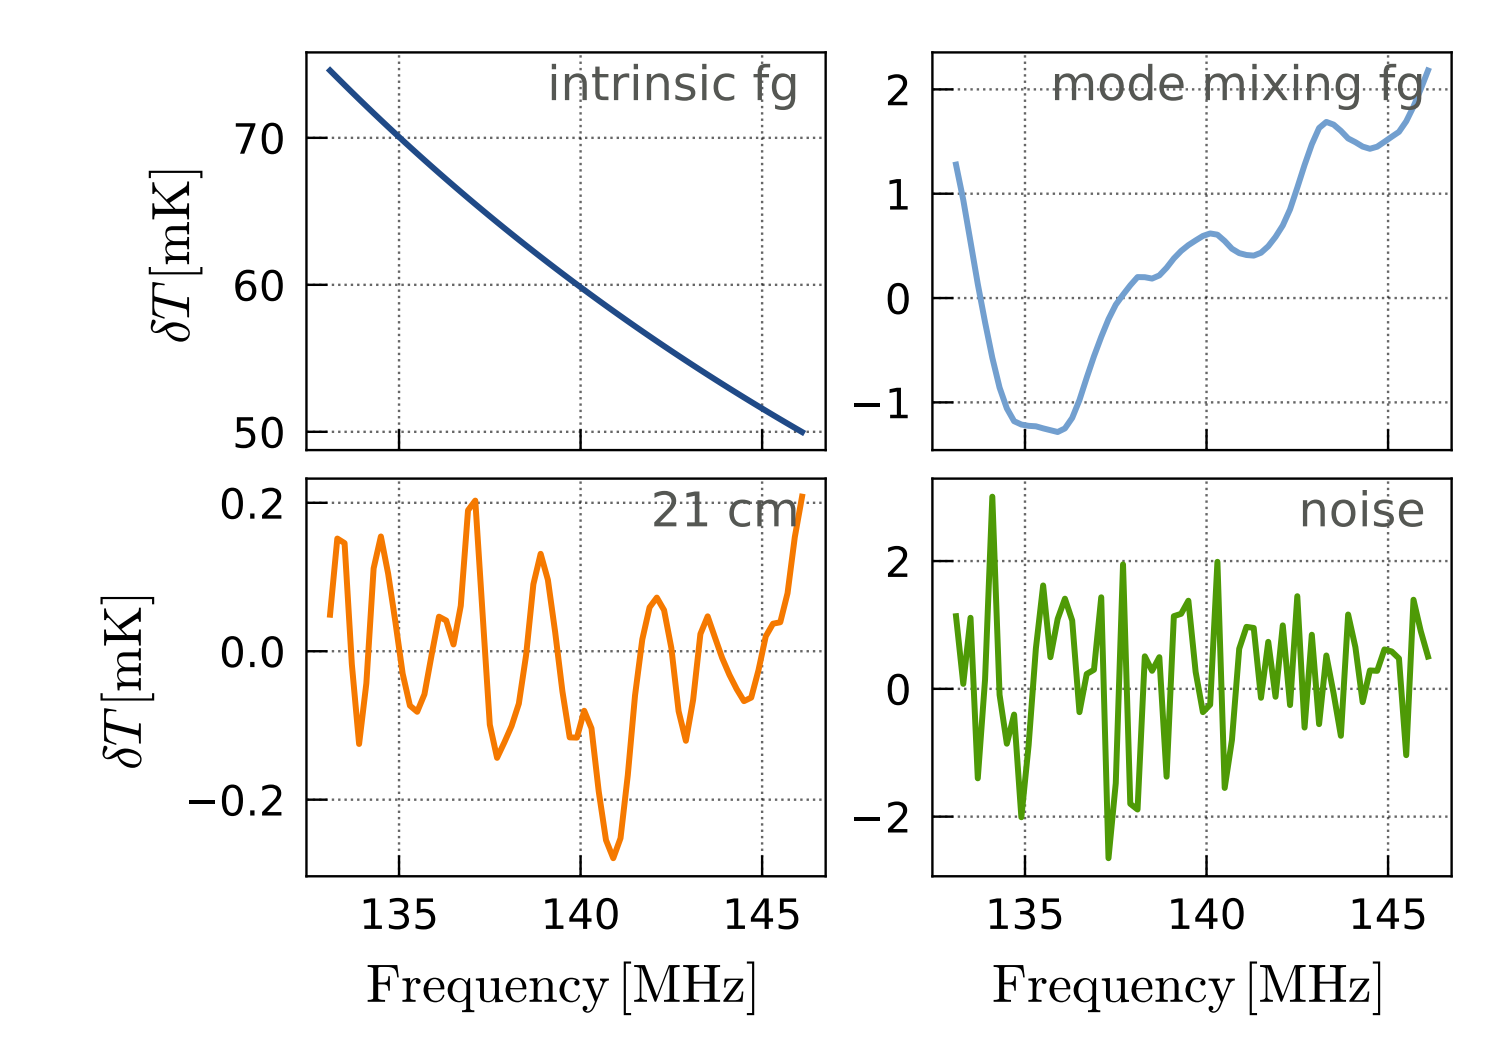
\includegraphics[width=0.9\textwidth]{Chapman_Jelic/Images/mertens_components.png}
\end{center}
    \caption{Simulated components of the observed signal, demonstrating that the smooth foreground signal is accompanied by an unsmooth mode mixing signal. GPR models each of these foreground components separately, making use of prior information about each component in the form of covariance functions. \textit{Reproduced from Mertens, Ghosh and Koopmans, (2018), MNRAS, 478(3):3640--3652}.}
    \label{fig:mertens_comp}
\end{figure}

 Blind Source Separation (BSS) methods have been used in Cosmic Microwave Background experiments \cite{PlanckI2018arXiv180706205P,PlanckIV2018} and their application to EoR data is a natural evolution. BSS methods are used across a wide range of fields in order to separate mixed signals into independent components. The data can be expressed in terms of the mixing model:

\begin{equation}
\mathbf{X} = \mathbf{A}\mathbf{S} + \mathbf{N}
\end{equation}

\noindent where $\mathbf{X}$ is the observed signal, $\mathbf{S}$ are the independent components of that signal, $\mathbf{N}$ is the noise and $\mathbf{A}$ is a matrix determining how the components are mixed, the `mixing matrix'. For an observation of $m$ frequency channels each constituting $t$ pixels and a foreground model of $n$ independent foreground components, the dimensions of these quantities are $\mathbf{X}$[$m$,$t$], $\mathbf{S}$[$n$,$t$], $\mathbf{N}$[$m$,$t$] and $\mathbf{A}$[$m$,$n$].

When this framework is applied to EoR data, the foregrounds are contained within $\mathbf{S}$[$n$,$t$] while the cosmological signal is contained along with the instrumental noise in $\mathbf{N}$[$m$,$t$]. The independent components of the foreground model are not directly related to the Galactic synchrotron, Galactic free-free and extragalactic foregrounds, but instead each independent component is potentially a mixture of all these physical foregrounds. This leaves the user without a physically motivated choice for the number of independent components, so that the number must be chosen empirically based on simulated data. Once a foreground model $\mathbf{A}\mathbf{S}$ has been determined this can then be subtracted from the observed signal, leaving the residual data as with the other methods.

\begin{figure}
\begin{center}
    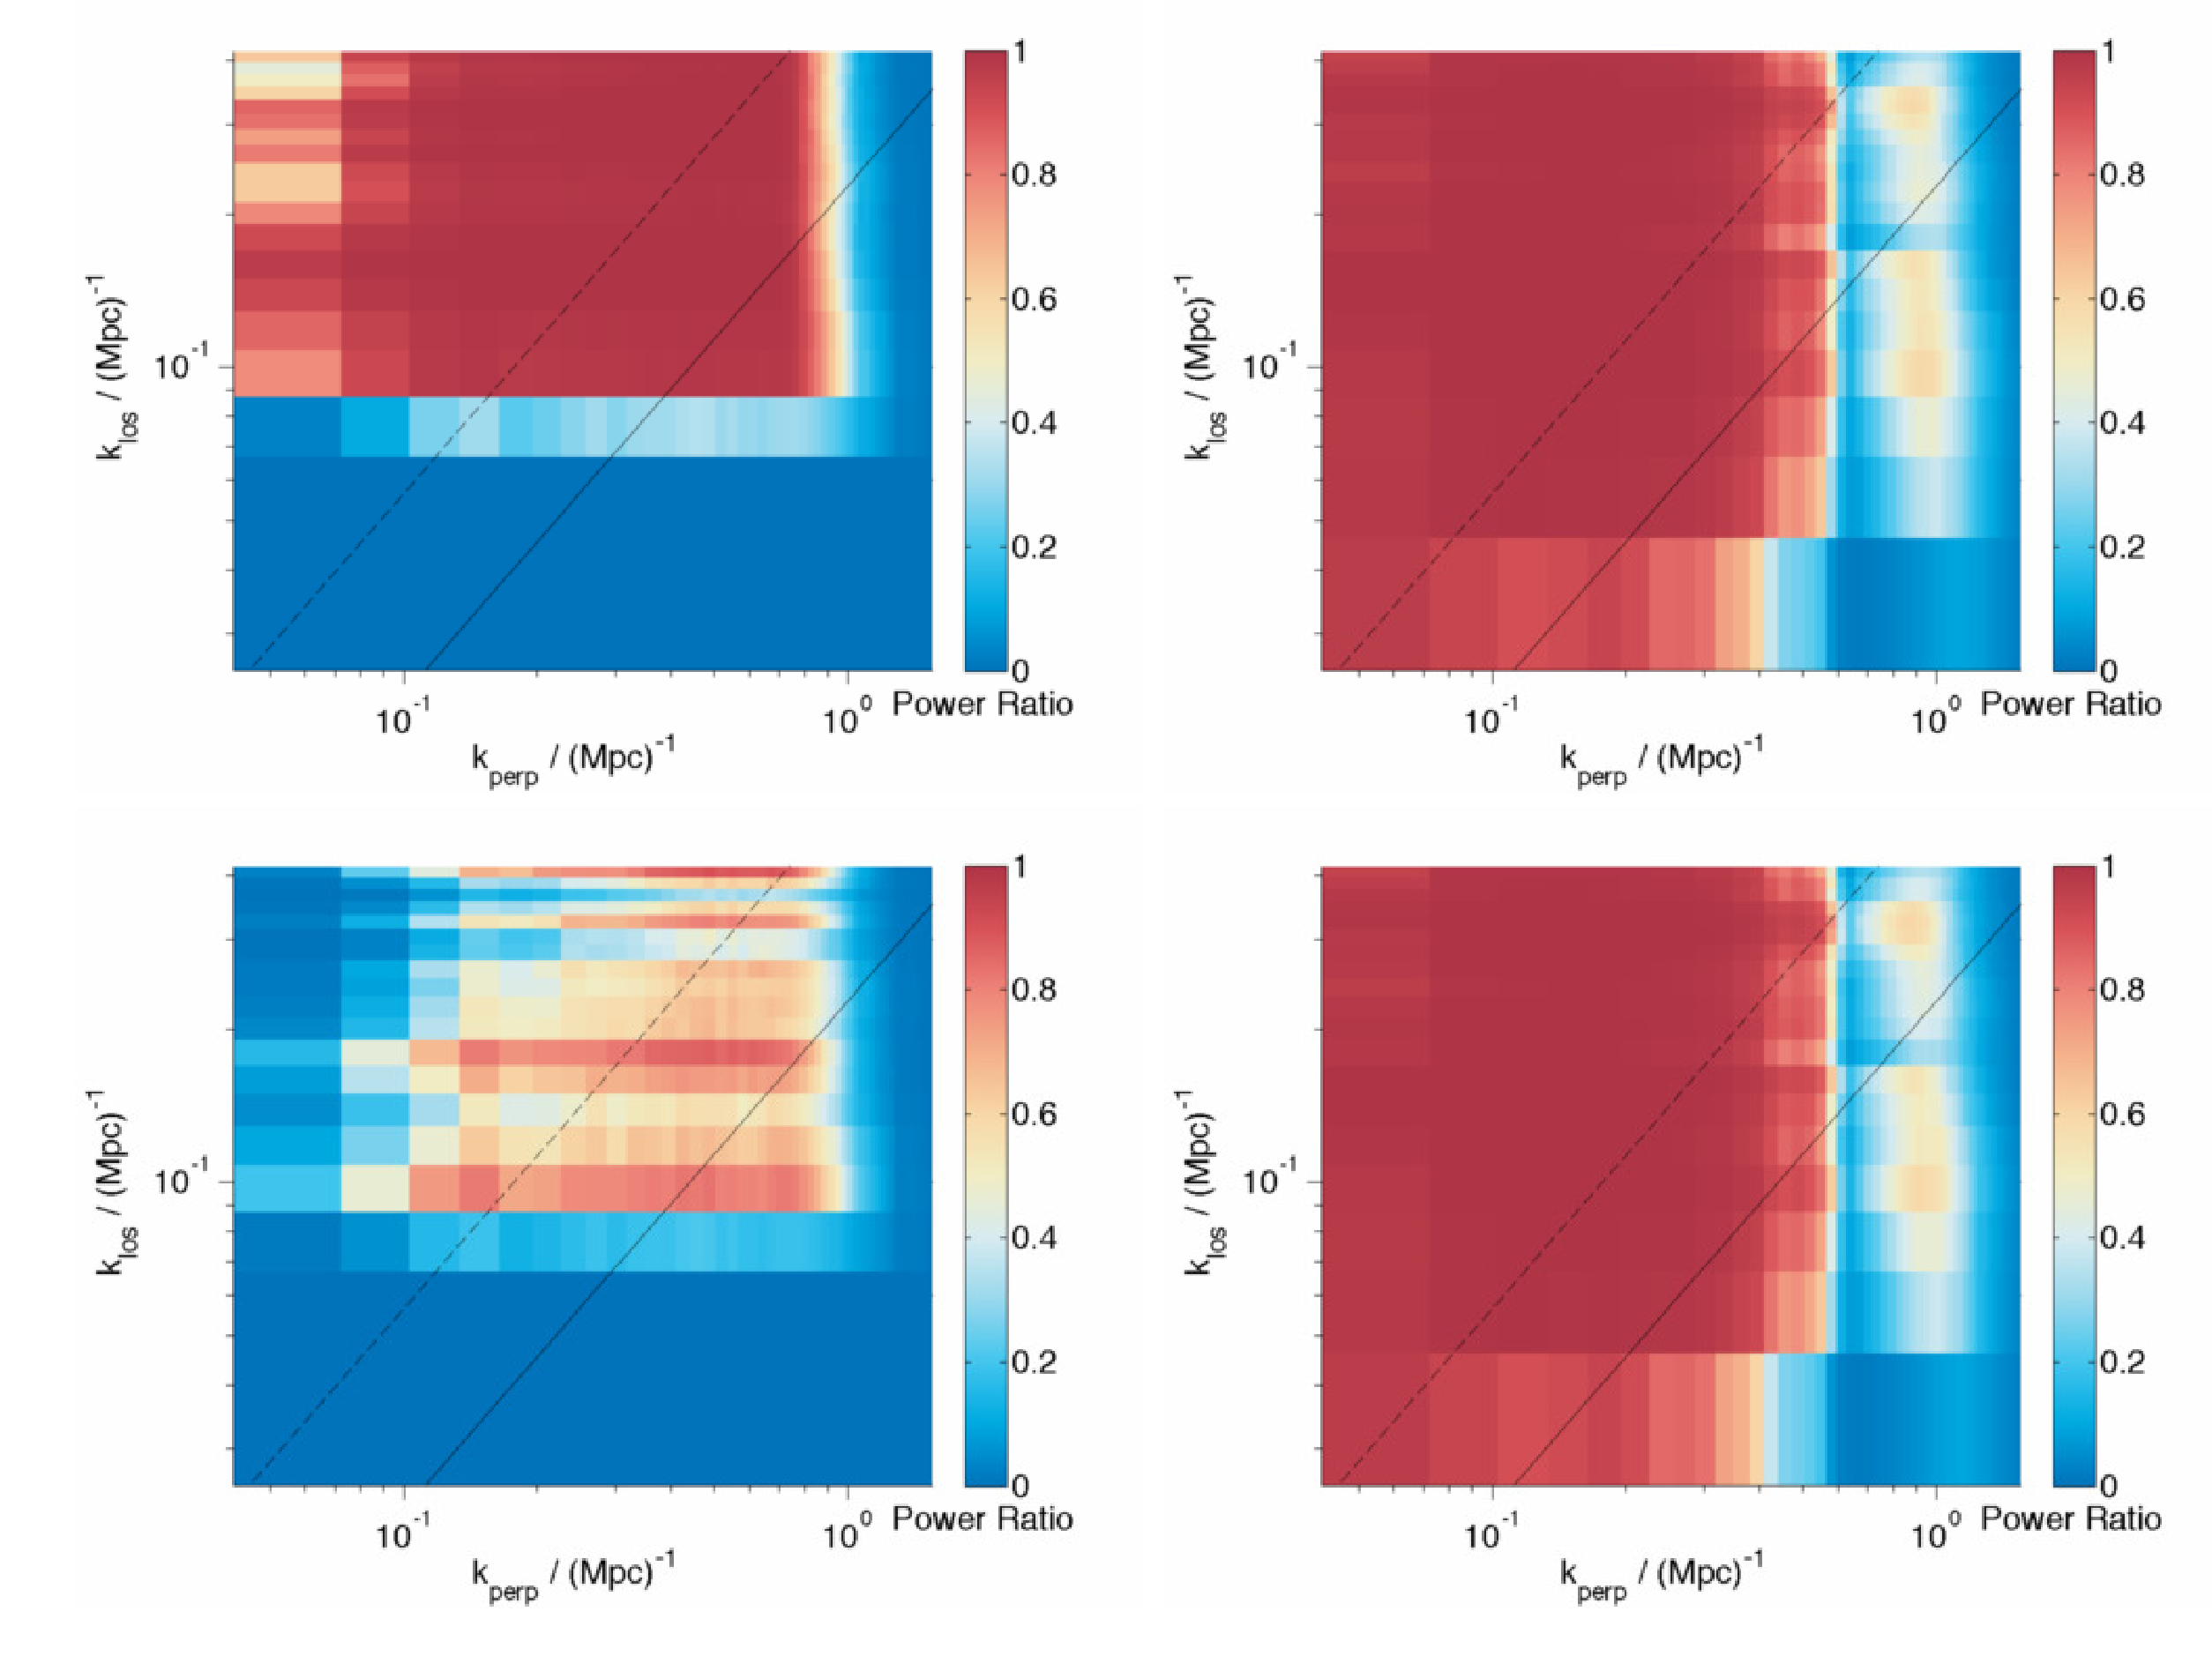
\includegraphics[width=0.9\textwidth]{Chapman_Jelic/Images/Em_window.png}
\end{center}
    \caption{The left column shows the ratio of the simulated components, (cosmological signal / (cosmological signal + foregrounds)), demonstrating that the area of the window free from foreground contamination is small when the foregrounds are unsmooth. The top row is where the foreground model has a random wiggle along the line of sight equal in magnitude to 0.1$\%$ of the foreground signal. The bottom row shows a 1$\%$ wiggle. On the right is the same ratio but with foreground fitting errors after foreground removal by GMCA instead of the simulated foregrounds, demonstrating that the method can open up the EoR window significantly even when the smoothness of the foregrounds is under threat. \textit{Reproduced from Chapman, Zaroubi et al. (2016), MNRAS, 458(3):2928--2939}.}
    \label{fig:Chap_window}
\end{figure}

The two BSS methods introduced for use on EoR data differ by their definition of independence. FastICA \cite{Chapman2012MNRAS.423.2518C,hyvarinen2004independent,hyvarinen1999fast} is a long-established independent component analysis technique which uses statistical independence to separate out the foreground components. FastICA constrains the different components by maximizing the negentropy of the signal components, utilising central limit theorem which states that the more independent components a signal contains, the more Gaussian the probability distribution function of that signal will be. In contrast, GMCA \cite{Bobin2016AA...591A..50B,bobin2015sparsity,Chapman2013MNRAS.429..165C,Bobin2008StMet...5..307B} is a method developed for use on CMB data that uses morphological diversity to separate out components. GMCA assumes that the data is represented in a sparse manner which can be achieved by a wavelet decomposition. With the independent components unlikely to have the same few non-zero basis coefficients in wavelet space, the method is able to separate out the components according to the differing sparse basis coefficient values. As with FastICA, we actually care little for the independent components individually, it is the combination of those as a whole which form the foreground model, with the method naturally separating out the decoherent noise and cosmological signal. In simulation both these methods have behaved well, opening up the EoR window into the lowest scales even when subjected to unsmooth foreground simulations, Fig. \ref{fig:Chap_window}. GMCA was used to achieve the current LOFAR upper-limit \cite{Patil2017ApJ...838...65P} but since then has not been able to remove the foregrounds down to the same level as, for example, GPR \cite{Mertens2018MNRAS.478.3640M}. The reason for this remains unknown and a full comparative analysis is currently underway. \cite{Mertens2018MNRAS.478.3640M} also expressed concern that because BSS methods are not based on defining the components in a statistical framework relating to the contributions from foregrounds and mode-mixing, they are not easily assessed for uncertainty and physical meaning. The blind methods are very useful as a separate check on results from what are extremely complex experiments, with many unknown unknowns. There is scope to move these methods towards a more parametric framework, perhaps constraining the mixing matrix columns according to the first-hand knowledge about the instrumental effects and foregrounds we have built up from the pathfinder telescopes. This is a similar philosophy as introduced by \cite{Bonaldi2015MNRAS.447.1973B} in Correlated Component Analysis (CCA). While still based on a mixing matrix framework, CCA is a parametric method which constrains the mixing matrix to represent power law behaviour over frequency, fixing the spectral index for a Galactic free-free contribution explicitly. 

While Wp smoothing, GMCA, GPR and FastICA are all labelled non-parametric in the literature, it is important to note than none of them are fully blind or indeed fully non-parametric. Each of them require the selection of parameters to define the fit: whether it is the smoothing parameter in Wp smoothing, or the number of independent components in GMCA and FastICA. So far these parameters have been chosen based on minimizing the foreground fitting error on simulated data, where the foreground model is known. A more robust method is to implement a Bayesian model selection model, as GPR does already. In addition, \cite{Gleser2008MNRAS.391..383G} developed a method based on the Bayesian maximum a posteriori probability (MAP) formalism, assuming priors for the smoothness of the contaminating radiation and for the correlation properties of the cosmological signal and \cite{Zhang2016ApJS..222....3Z} introduced HIEMICA (HI Expectation Maximization Independent Component Analysis), an extension of ICA with a fully Bayesian inference of the foreground power spectra, allowing their separation from the cosmological signal power spectra. Machine learning has also been applied in an effort to seek a foreground model defined by the data itself \cite{Li2019MNRAS.485.2628L}. There are now a multitude of non-parametric foreground subtraction methods available which have each proved their own principle on simulated, and in the case of GPR and GMCA, observed data. Now we know the constraints of the instrument much better, work on the relative advantages and disadvantages of all these approaches are a logical next step.

\subsection{Residual Error Subtraction}
The final stage of foreground mitigation is residual error subtraction \cite{Morales2006ApJ...648..767M,Morales2004ApJ...615....7M}. The residual foreground mitigation errors from the previous two stages (bright source subtraction and diffuse foreground mitigation) produce distinct shapes in the spherical power spectrum, Fig. \ref{fig:ressub}. One can take the spherical power spectrum of the residual data and apply a multi-parameter fit according to the foreground residual and EoR template power spectrum. This allows a final cleaning of residual foreground contamination. \cite{Morales2006ApJ...648..767M} also notes that ``because the residual error subtraction relies on the statistical characteristics of the subtraction errors, the foreground removal steps become tightly linked and we must move from focusing on individual subtraction algorithms to the context of a complete foreground removal framework." This statement leads us neatly to the conclusion of this chapter.

\begin{figure}
\begin{center}
    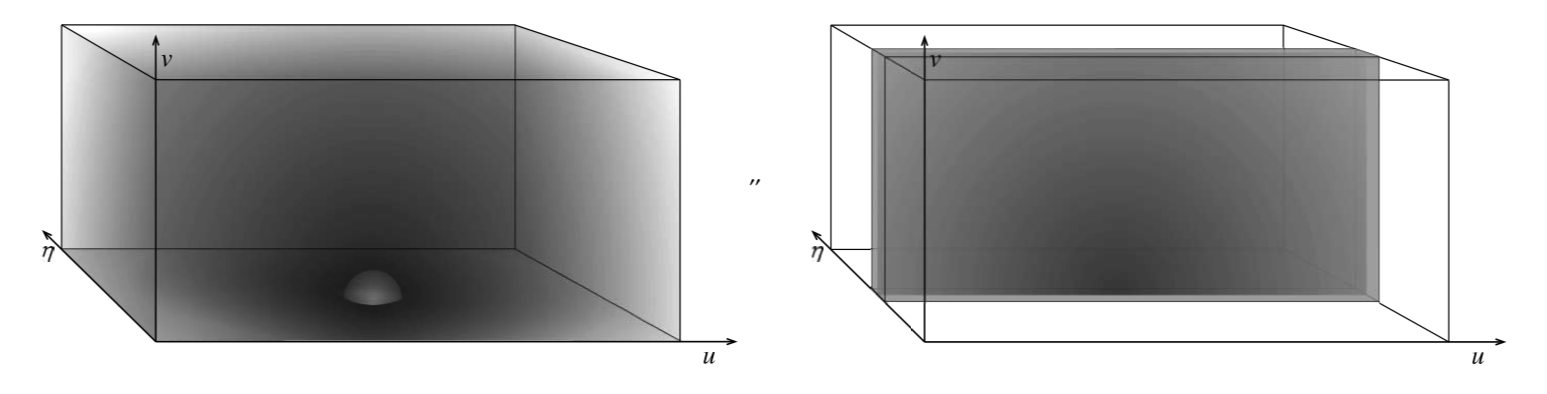
\includegraphics[width=0.9\textwidth]{Chapman_Jelic/Images/res_sub.png}
\end{center}
    \caption{The 3D spherical power spectrum of the EoR signal (left), and an example residual foreground signal template (right), where zero is at the centre of the bottom face of the cuboid. The foreground signal displays a separable-axial symmetry while the EoR signal has a symmetric power spectrum. This contrast allows a further separation stage in order to clean the foreground fitting errors which have accumulated from the previous two stages of bright source subtraction and diffuse foreground mitigation. \textit{Reproduced from Morales, Bowman, and Hewitt (2006), ApJ, 648(2):767--773}.}
    \label{fig:ressub}
\end{figure}

\subsection{Polarization leakage}\label{sec:leakage}
One of the challenges in calibration is to minimise leakage of polarization signals in total intensity. Otherwise, the polarization leakage can contaminate the cosmological 21-cm signal. 
A level of contamination depends strongly on characteristics of a radio telescope, its calibration strategy, and of polarized emission itself.

Antennas in the low-frequency radio telescopes are dipoles. Dipoles usually come in pairs. In each pair dipoles are orthogonal to each other and each dipole is sensitive to a certain polarization. Since antennas are also fixed to the ground, it is not possible to preform observations like with the traditional dish-like radio telescopes, where the tracking  is done by steering the dish. Here, the sources are tracked by the beam-forming or simply the observation is done in a drift-scan mode. Depending on the position of the sources in the sky, the sources will see different projections of dipoles. If this geometrical projection  is not corrected during the calibration, or the modelling of and correction for the beam polarization is not accurate, polarized signals can leak to total intensity and vice versa. 

\begin{figure}[!t]
   \centering	
   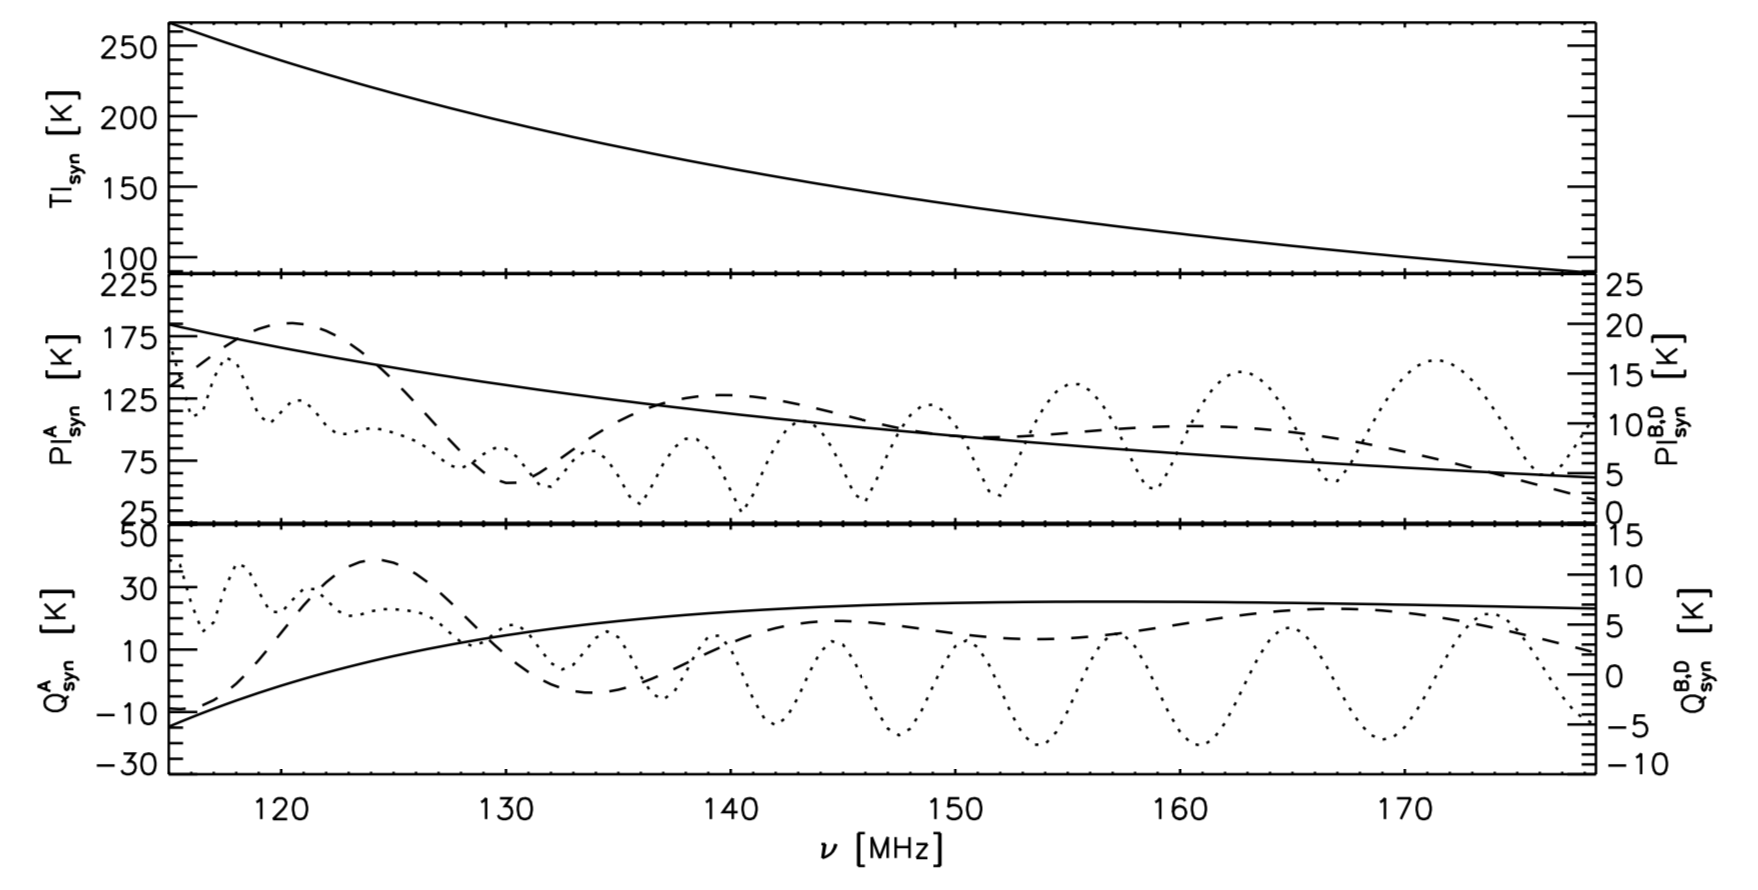
\includegraphics[width=0.8\textwidth]{Chapman_Jelic/Images/leakage.png}
    \caption{Galactic synchrotron emission given as a function of frequency in total intensity (Stokes I, $T^I_{b,FG}$) and polarization (Stokes Q and U, $T^{Q,U}_{b,FG}$). The spectra are generated by Jeli\'c simulations \cite{jelic10, jelic08}. Polarized emission can have a very complex frequency dependence compared to the plain power-law behaviour in the total intensity, due to distinct Faraday rotation and depolarization at low-radio frequencies (see Sec.~\ref{sec:polarfg}). If polarized emission consists of the multiple Faraday components and/or if some of the components are at $\Phi\gtrsim15~{\rm rad~m^{-2}}$ (example B vs. A) this can create a leaked signal in total intensity that looks like the cosmological 21cm signal ($T^I_{b,21}$, in this case generated by 21cmFAST \cite{mesinger11}).  }
\label{fig:leakage}
\end{figure}

Since the polarized emission from the Milky Way can have a very complex frequency dependence, a leakage of this signal to the total intensity can contaminate the cosmological 21-cm signal, making extraction and analysis more demanding (\cite{jelic10, moore13, spinelli18} and see Fig.~\ref{fig:leakage}). A number of studies addressed this problem for different low-frequency radio telescopes: LOFAR \cite{asad18, asad16, asad15},  MWA \cite{sutinjo15} and PAPER \cite{kohn16, nunhokee17}.  Although the assessed polarization leakage in these studies is not limiting current  observations, it will become relevant once we reach a better sensitivity in the data. This will be especially the case for future 21 cm experiments, like HERA and SKA. 

Most of the observed structures appear at Faraday depths $|\Phi|\lesssim15~{\rm rad~m^{-2}}$, which measures the amount of Faraday rotation by
intervening interstellar medium (see Sec.~\ref{sec:polarfg}). Relatively small Faraday depths indicate polarized emission that fluctuates along frequency on scales  larger than 
the expected cosmological 21-cm signal  in total intensity (e.g. \cite{moore13}). Thus, associated leaked signals can be in principle mitigated, as it was shown in the case of a simple and  thin Faraday screen \cite{geil11}. On the contrary, polarized emission at Faraday depths $|\Phi|\gtrsim15~{\rm rad~m^{-2}}$ can introduce frequency dependent signals, which if leaked can resemble the cosmological signal and make foreground mitigation difficult.  Prior to the CD/EoR observations, it is therefore important to asses the properties of Galactic polarized emission in targeted region of the sky. 



\section{Conclusions}
The foreground emission of our Galaxy and extragalactic radio sources dominates over the whole frequency range of the cosmological 21cm experiments. In order to mitigate the foreground emission from the data we need to study and constrain its properties in great details. Thanks to the observations with LOFAR and MWA this is becoming possible.

The current EoR experiments are now modelled and constrained to an excellent degree but during that process there has been a blurring of boundaries between the analysis modules. The calibration stage, once assumed to mitigate foreground point sources only, can erroneously suppress diffuse foregrounds \cite{Patil2016MNRAS.463.4317P} and the mode-mixing of the instrument has required more complex modelling as wide-field effects have become apparent \cite{Thyagarajan2015ApJ...807L..28T}. There are a promising number of foreground mitigation techniques now available providing the necessary diversity of pipelines necessary for verifying the first detection. So far, there has not been a wide-reaching comparison of all of these methods or a complete assessment of their strengths and weaknesses for recovery of the different aspects of the EoR signal such as power spectra or images. Foreground subtraction, suppression and avoidance are now used in combination in the experimental pipelines and the further development of the best combination for these methods will provide an exciting area of research in the next decade.

\bibliographystyle{plain}
\bibliography{References}


%\chapter{Theoretical Framework: The Fundamentals of the 21-cm Line}

\begin{bf}
  \author{Steven R. Furlanetto}\\

  Abstract\\

We review some of the fundamental physics necessary for computing the highly-redshifted spin-flip background. We first discuss the radiative transfer of the 21-cm line and define the crucial quantities of interest. We then review the processes that set the spin temperature of the transition, with a particular focus on Wouthuysen-Field coupling, which is likely to be the most important process during and after the Cosmic Dawn. Finally, we discuss processes that heat the intergalactic medium during the Cosmic Dawn, including the scattering of Lyman-$\alpha$, cosmic microwave background, and X-ray photons.
\end{bf}

\section{Radiative Transfer of the 21-cm Line} \label{rt-21cm}

Consider a spectral line labeled by 0 (the lower level) and 1 (the upper level). The radiative transfer equation for the specific intensity $I_\nu$ of photons at the relevant frequency is
\begin{equation}
{dI_\nu\over d\ell}={\phi(\nu) h\nu\over 4\pi}\left[n_1 A_{10} -
\left(n_0 B_{01} -n_1 B_{10}\right)I_\nu\right],
\label{rad}
\end{equation}
where $d\ell$ is a proper path length element, $\phi(\nu)$ is the line profile function, $n_i$
denotes the number density of atoms at the different levels, and $A_{ij}$ and $B_{ij}$ are the Einstein coefficients for the relevant transition (here $i$ and $j$ the initial and final states, respectively). For the 21-cm line, the line frequency is $\nu_{21} = 1420.4057$~MHz. The Einstein relations associate the radiative transition rates via $B_{10}=(g_0/g_1)B_{01}$ and $B_{10}=A_{10}(c^2/2 h\nu^3)$, where $g$ is the spin degeneracy factor of each state. For the 21-cm transition, $A_{10}=2.85\times 10^{-15} \ {\rm s^{-1}}$ and $g_1/g_0=3$.

The relative populations of hydrogen atoms in the two spin states determine the {\bf spin temperature}, $T_S$, through the relation
\begin{equation}
\left({n_1\over n_0}\right)=\left({g_1 \over g_0}\right)
\exp\left\{ {-T_*\over T_S}\right\}, 
\end{equation}
where $T_* \equiv E_{10} /k_B=68$~mK is equivalent to the transition energy $E_{10}$. In almost all physically plausible situations,  $T_\star$ is much smaller than any other temperature, including $T_S$, so all the exponentials in temperature can be Taylor expanded to leading order with high accuracy. Note, however, that $T_S$ implicitly assumes that the level populations can be described by a single temperature -- independent of each atom's velocity. In detail, velocity-dependent effects must be considered in certain circumstances \cite{hirata07}.

It is conventional to replace $I_{\nu}$ by the equivalent {\bf brightness temperature}, $T_b(\nu)$, required of a blackbody radiator (with spectrum $B_{\nu}$) such that $I_{\nu}=B_{\nu}(T_b)$. In the low frequency regime relevant to the 21 cm line, the Rayleigh-Jeans formula is an excellent approximation to the Planck curve, so $T_b(\nu)\approx I_{\nu} \, c^2/2k_B{\nu}^2$.

In this limit, the equation of radiative transfer  along a line of sight through a cloud of uniform excitation temperature $T_S$ becomes
\begin{equation}
T_b'(\nu) = T_{S}(1-e^{-\tau_{\nu}})+T_R'(\nu)e^{-\tau_{\nu}}
\label{eq:rad_trans}
\end{equation}
where $T_b'(\nu)$ is the emergent brightness measured at the cloud and at redshift $z$, the {\bf optical depth}  $\tau_\nu \equiv \int d s \, \alpha_{\nu}$ is the integral of the absorption coefficient ($\alpha_{\nu}$)  along the ray through the cloud, $T_R'$ is the brightness of the background radiation field incident on the cloud along the ray, and $s$ is the proper distance. Because of the cosmological redshift, for the 21-cm transition an observer will measure an apparent brightness at the Earth of $T_b(\nu) = T_b'(\nu_{21})/(1+z)$, where the observed frequency is $\nu=\nu_{21}/(1+z)$. Henceforth we will work in terms of these observed quantities.

The absorption coefficient is related to the Einstein coefficients via
\begin{equation}
\alpha = \phi(\nu) {h \nu \over 4 \pi} (n_0 B_{01} - n_1 B_{10}).
\end{equation}
Because all astrophysical  applications have $T_S \gg T_*$, approximately three of four atoms find themselves in the excited state ($n_0 \approx n_1/3$).  As a result, the stimulated emission correction represented by the first term is significant.  

The fundamental observable quantity is the change in brightness temperature induced by the 21-cm line by a patch of the intergalactic medium (IGM), relative to the incident radiation field. In most models that incident field is simply the cosmic microwave background, although if other sources create a low-frequency radio background at very high redshifts, or if there is a particular source behind the IGM patch along the line of sight from the observer, a larger radio background may exist.

Consider photons incident on the patch from this background. If any redshift into resonance with the 21-cm line, they can interact with the cloud -- but only for a short time, as they will redshift out of resonance as the Universe continues to expand. Thus the Hubble expansion rate sets an effective path length through the cloud, simply equal to the distance the photon travels while it remains within the line profile. The total absorption can be calculated by integrating the IGM density across this interval, in an exactly analogous procedure to the calculation of the Gunn-Peterson Lyman-$\alpha$ optical depth \cite{field59-obs, gunn65, scheuer65}. The result is
\begin{eqnarray}
\tau_{10} & = & \frac{3}{32 \pi} \, \frac{h c^3 A_{10}}{k_B T_S \nu_{10}^2} \, \frac{x_{\rm HI} n_{\rm H}}{(1+z) \, (d v_\parallel/d r_\parallel)}  \label{eq:optdepthcosmo} \\
 & \approx  & 0.0092 \, (1+\delta) \, (1+z)^{3/2}\, \frac{x_{\rm HI}}{T_S} \, \left[ \frac{H(z)/(1+z)}{d v_\parallel/d r_\parallel} \right],
\label{optdepthcosmo-approx}
\end{eqnarray}
where $n_H$ is the hydrogen number density, $x_{\rm HI}$ is the neutral fraction, $dv_\parallel/dr_\parallel$ is the velocity gradient along the line of sight (here scaled to the Hubble flow). In the second part,$T_S$ is in Kelvins, and we have scaled the density to the mean value by writing $n_H = \bar{n}_H^0 (1+z)^3 (1 + \delta)$, where $\bar{n}_H^0$ is the mean comoving density today.

In most circumstances, the CMB provides the background radiation source, for which with temperature $T_\gamma(z)$. Then $T_R' = T_{\gamma}(z)$, so that  we are observing the contrast between high-redshift hydrogen clouds and the CMB.   Because the optical depth is so small, we can then expand the exponentials in equation~(\ref{eq:rad_trans}), and
\begin{eqnarray}
& T_b(\nu) & \approx \frac{T_S-T_{\gamma}(z)}{1+z}\;\tau_{\nu_0} 
\label{eq:dtbone} \\
& \approx & 9\;x_{\rm HI}(1+\delta) \, (1+z)^{1/2}\, \left[1-\frac{T_{\gamma}(z)}{T_S}\right] \, \left[ \frac{H(z)/(1+z)}{d v_\parallel/d r_\parallel} \right] \ \mbox{mK}.
\label{eq:dtb}
\end{eqnarray}
Thus $T_b < 0$ if $T_S < T_{\gamma}$, yielding an absorption signal; otherwise it appears in emission relative to the CMB. Both regimes are likely important for the high-$z$ Universe. Note that $T_b$ saturates if $T_S \gg T_{\gamma}$, but the absorption can become arbitrarily large if $T_S \ll T_{\gamma}$.  The observability of the 21 cm transition therefore hinges on the spin temperature; we will next describe the mechanisms that control that factor.

\section{The Spin Temperature} \label{spin-temp}

Three competing processes determine $T_S$: {\it (i)} absorption of CMB photons (as well as stimulated emission); {\it (ii)} collisions with other particles; and{\it (iii)} scattering of UV photons.  In the presence of the CMB
alone, the spin states reach thermal equilibrium ($T_S=T_{\gamma}$) on a time-scale of $\sim T_*/(T_\gamma A_{10}) = 3 \times 10^5 (1+z)^{-1}$ yr -- much shorter than the age of the Universe at all redshifts after cosmological recombination, indicating that CMB coupling establishes itself rapidly. Indeed all the relevant processes adjust on very short timescales (compared to the Hubble time) so equilibrium is an excellent approximation.

However, the other two processes break this coupling. We let $C_{10}$ and $P_{10}$ be the de-excitation rates (per atom) from collisions and UV scattering, respectively.  We also let $C_{01}$ and $P_{01}$ be the
corresponding excitation rates.  In equilibrium, the spin temperature is then
determined by
\begin{equation}
n_1 \left( C_{10} + P_{10} + A_{10} + B_{10} I_{\rm CMB} \right) = n_0 \left( C_{01} + P_{01} + B_{01} I_{\rm CMB} \right),
\label{eq:detbal}
\end{equation}
where $I_{\rm CMB}$ is the specific intensity of CMB photons at $\nu_{21}$.  With the Rayleigh-Jeans approximation, equation (\ref{eq:detbal}) can be rewritten as
\begin{equation}
T_S^{-1} = \frac{T_\gamma^{-1} + x_c T_K^{-1} + x_\alpha T_c^{-1}}{1 + x_c + x_\alpha},
\label{eq:xdefn}
\end{equation}
where $x_c$ and $x_\alpha$ are coupling coefficients for collisions and UV scattering, respectively, and $T_K$ is the gas kinetic temperature.  Here we have used the principle of detailed balance through the relation
\begin{equation}
\frac{C_{01}}{C_{10}} = \frac{g_1}{g_0} e^{-T_\star/T_K} \approx 3 \left( 1 - \frac{T_\star}{T_K} \right).
\label{eq:c01db}
\end{equation}
We have also \emph{defined} the effective color temperature of the UV radiation field $T_c$ via
\begin{equation}
\frac{P_{01}}{P_{10}} \equiv 3 \left( 1 - \frac{T_\star}{T_c} \right).
\label{eq:tcolor}
\end{equation}
In the limit in which $T_c \rightarrow T_K$ (usually a good approximation), equation~(\ref{eq:xdefn}) may be written 
\begin{equation}
1 - \frac{T_\gamma}{T_S} = \frac{x_c + x_\alpha}{1 + x_c + x_\alpha} \, \left( 1 - \frac{T_\gamma}{T_K} \right).
\label{eq:xdefn-tfac}
\end{equation}

We must now calculate $x_c$,  $x_\alpha$, and $T_c$, which we shall do in the next subsections.

\subsection{Collisional Coupling} \label{coll}

We will first consider collisional excitation and de-excitation of the hyperfine levels, which become important in dense gas.  The coupling coefficient for collisions with species $i$ is
\begin{equation}
x_c^i \equiv  \frac{C_{10}^i}{A_{10}} \, \frac{T_\star}{T_\gamma} = \frac{n_i \, \kappa_{10}^i}{A_{10}} \, \frac{T_\star}{T_\gamma},
\label{eq:xcdefn}
\end{equation}
where $\kappa_{10}^i$ is the rate coefficient for collisional spin de-excitation in collisions (with units of cm$^3$ s$^{-1}$).  The total $x_c$ is the sum over all relevant species $i$, including collisions with (1) neutral hydrogen atoms, (2) free electrons, and (3) protons.  

These rate coefficients can be calculated by the quantum mechanical cross sections of the relevant processes \cite{zygelman05, furl07-electron, furl07-proton}. We will not list them in detail but show the rates in Figure~\ref{fig:collrates}.  Although the atomic cross-section is small, in the unperturbed IGM collisions between neutral hydrogen atoms nearly always dominate these rates because the ionized fraction is small.  Free electrons can be important in partially ionized gas; collisions with protons are only important at the lowest temperatures.

%%%%%: FIGURE: Collision rates
\begin{figure}[]
\begin{center}
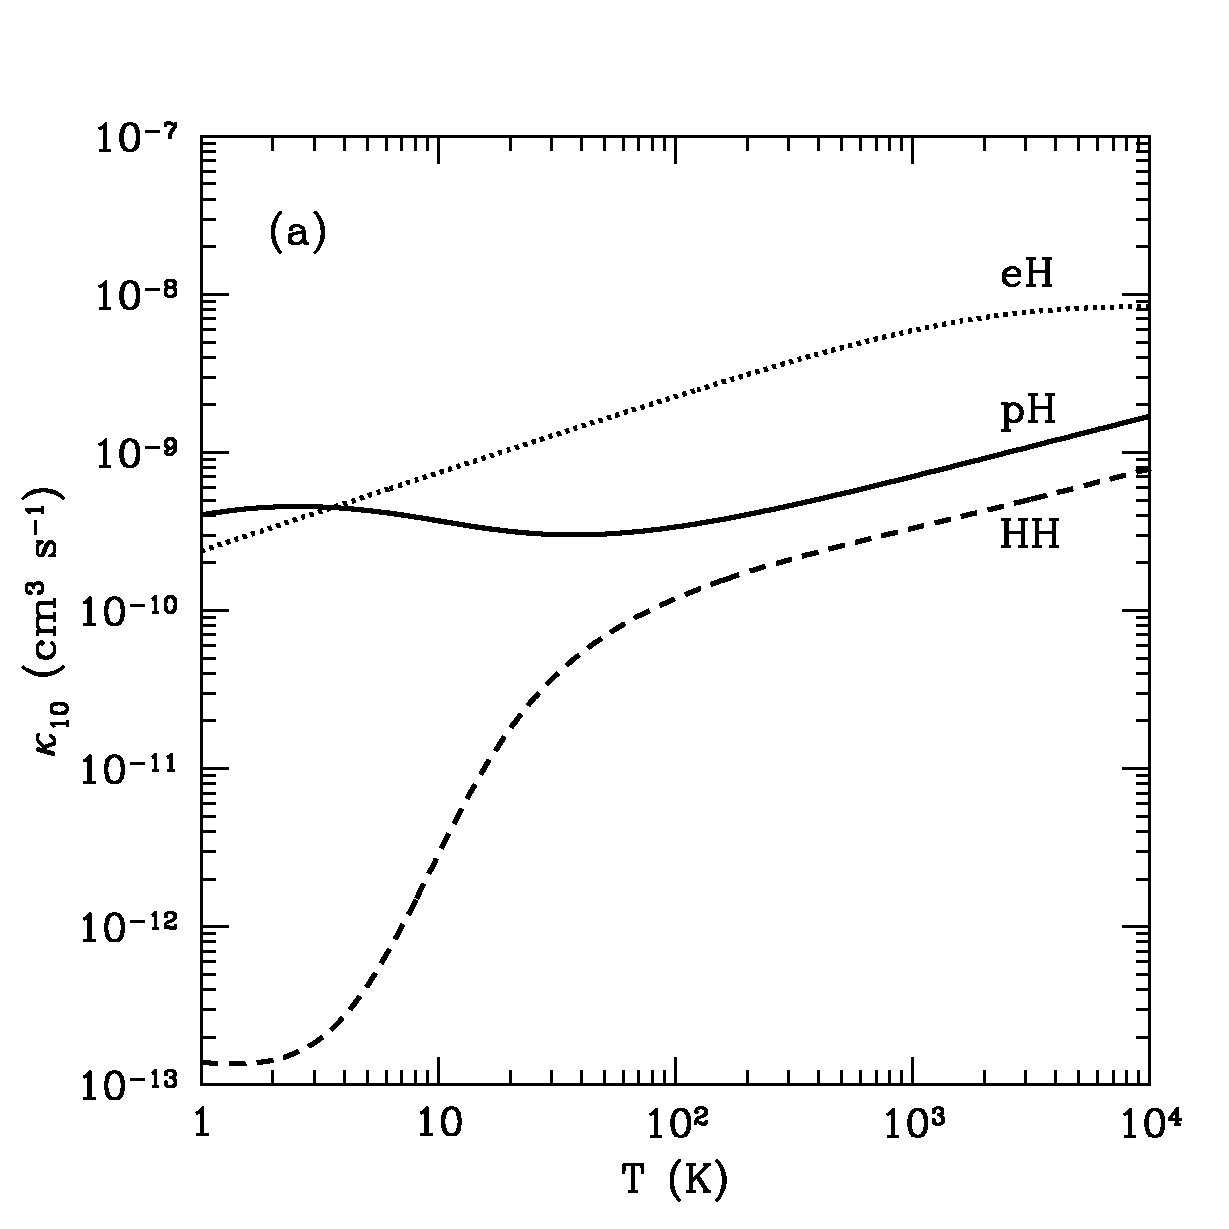
\includegraphics[width=0.5\textwidth]{Furlanetto/figure2-1}
\end{center}
\caption{De-excitation rate coefficients for H-H collisions (dashed
line), H-e$^-$ collisions (dotted line), and H-p collisions (solid
line).  Note that the net rates are also proportional to the densities
of the individual species, so H-H collisions still dominate in a
weakly-ionized medium. From \cite{furl07-proton}.}
\label{fig:collrates}
\end{figure}

Given the densities relevant to the IGM, collisional coupling is quite weak in a nearly neutral, cold medium.  Thus, the local density must be large in order for this process to effectively fix $T_S$. A convenient estimate of their
importance is the critical overdensity, $\delta_{\rm coll}$, at which
$x_c=1$ for H--H collisions:
\begin{equation}
1 + \delta_{\rm coll} = 0.99 \, \left[ \frac{\kappa_{10}(88 \ \mbox{K})}{\kappa_{10}(T_K)} \right] \, \left( \frac{0.023}{\Omega_b
    h^2} \right) \, \left( \frac{70}{1+z} \right)^2,
\label{eq:dcoll}
\end{equation}
where 88~K is the expected IGM temperature at $1+z=70$.\footnote{Note that this is \emph{smaller} than the CMB temperature at this time, because the IGM gas cools faster (due to adiabatic expansion) once Compton scattering becomes inefficient at $z \sim 150$.}  In the standard picture, at redshifts $z < 70$, $x_c \ll 1$ and $T_S \rightarrow T_{\gamma}$; by $z \sim 30$ the IGM essentially becomes invisible.  However, $\kappa_{10}$ is extremely sensitive to $T_K$ in this low-temperature regime.  If the Universe is somehow heated above the fiducial value, the threshold density can remain modest: $\delta_{\rm coll} \approx 1$ at $z=40$ if $T_K=300$~K.

\subsection{The Wouthuysen-Field Effect} \label{wf}

We must therefore appeal to a different mechanism to render the 21-cm transition visible during the era of the first galaxies.  This is known as the {\bf Wouthuysen-Field mechanism} (named after the Dutch physicist Siegfried
Wouthuysen and Harvard astrophysicist George Field who first explored it \cite{wouthuysen52, field58}). Figure~\ref{fig:wf} illustrates the effect. This shows the hyperfine sub-levels of the $1S$ and $2P$ states of HI and the permitted transitions between them.  Suppose a hydrogen atom in the hyperfine singlet state absorbs a Lyman-$\alpha$ photon.  The electric dipole selection rules allow $\Delta F=0,1$ except that $F=0 \rightarrow 0$ is prohibited (here $F$ is the total angular momentum of the atom).  Thus the atom must jump to either of the central $2P$ states.  However, these same rules now allow electrons in either of these excited states to decay to the $_1S_{1/2}$ triplet level.\footnote{Here we use the notation $_F L_J$, where $L$ and $J$ are the orbital and total angular momentum of the electron.}  Thus, atoms can change hyperfine states through the absorption and spontaneous re-emission of a Lyman-$\alpha$ photon (or indeed any Lyman-series photon; see below).

%%%%%: FIGURE: W-F levels
\begin{figure}[]
\begin{center}
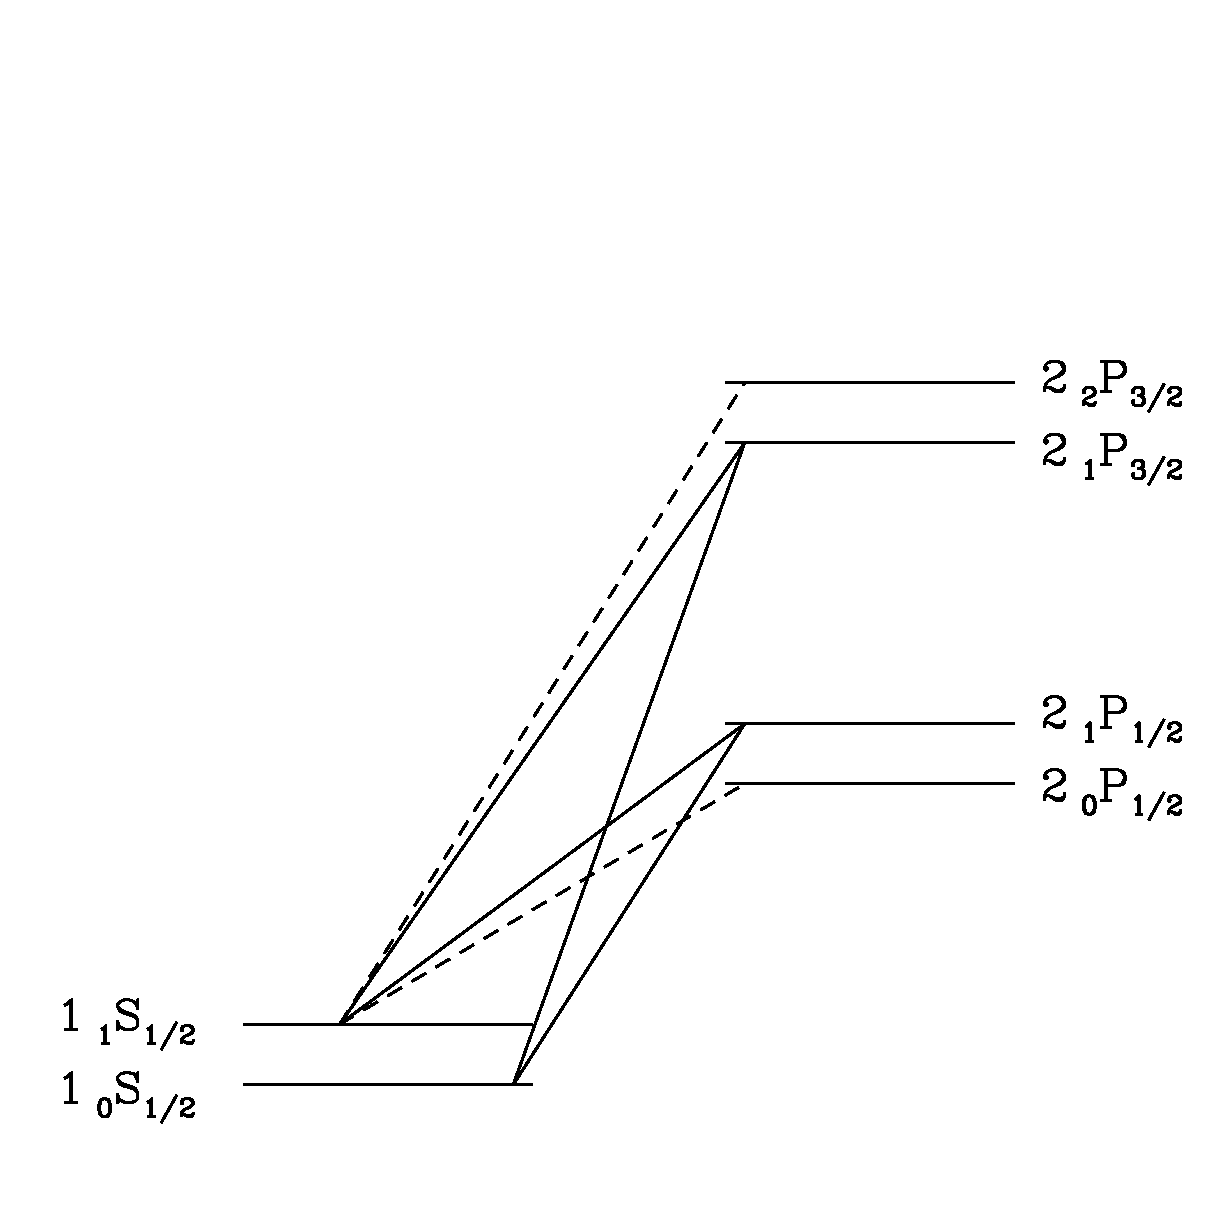
\includegraphics[width=0.6\textwidth]{Furlanetto/figure2-2}
\end{center}
\caption{Level diagram illustrating the Wouthuysen-Field effect.  We show the hyperfine splittings of the $1S$ and $2P$ levels.  The solid lines label transitions that can mix the ground state hyperfine levels, while the dashed lines label complementary allowed transitions that do not participate in mixing.  From \cite{pritchard06}.}
\label{fig:wf}
\end{figure}

The Wouthuysen-Field coupling rate depends ultimately on the total rate (per atom) at which Lyman-$\alpha$ photons scattered through the gas,
\begin{equation}
P_\alpha = 4 \pi \sigma_0 \int d \nu \, J_\nu(\nu) \phi_\alpha(\nu),
\label{eq:palpha}
\end{equation}
where $\sigma_\nu \equiv \sigma_0 \phi_\alpha(\nu)$ is the local Lyman-$\alpha$ absorption cross section, $\sigma_0 \equiv (\pi \, e^2/m_e \, c) f_{\alpha}$, $f_\alpha=0.4162$ is the oscillator strength of the Lyman-$\alpha$ transition, $\phi_\alpha(\nu)$ is the Lyman-$\alpha$ absorption profile, and $J_\nu$ is the angle-averaged specific intensity of the background radiation field.\footnote{By convention, we use the specific intensity in units of photons cm$^{-2}$ Hz$^{-1}$ s$^{-1}$ sr$^{-1}$ here, which is conserved during the expansion of the Universe (whereas a definition in terms of energy instead of photon number is subject to redshifting).}   

Transitions to higher Lyman-$n$ levels have similar effects \cite{hirata06, pritchard06}. Suppose that a UV photon redshifts into the Lyman-$n$ resonance as it travels through the IGM.  After absorption, it can either scatter (by the electron decaying directly to the ground state) or cascade through a series of intermediate levels and produce a sequence of photons.  The direct decay probability for any level is $\sim 0.8$, so a Lyman-$n$ photon will typically scatter $N_{\rm scatt} \approx (1-P_{nP\rightarrow1S})^{-1} \sim 5$ times before instead initiating a decay cascade.  In contrast, Lyman-$\alpha$ photons scatter hundreds of thousands of times before being destroyed, usually be redshifting all the way across the (very wide) Lyman-$\alpha$ profile.  As a result, coupling from the direct scattering of Lyman-$n$ photons is suppressed compared to Lyman-$\alpha$ by a large factor.

However, Lyman-$n$ photons can still be important because of their cascade products, as shown in Figure~\ref{fig:lygamma}.  Following Lyman-$\beta$ absorption, the only permitted decays are to the ground state (regenerating a Lyman-$\beta$ photon and starting the process again) or to the $2S$ level.  The H$\alpha$ photon produced in the $3P \rightarrow 2S$ transition (and indeed any photon produced in a decay to an excited state) escapes to infinity. Thus the atom will eventually find itself in the $2S$ state, which decays to the ground state via a forbidden two photon process with $A_{2S\rightarrow1S}=8.2$~s$^{-1}$.  These photons will also escape to infinity, so coupling from Lyman-$\beta$ photons can be completely neglected.\footnote{In a medium with very high number density, atomic collisions can mix the two angular momentum states, but that process is unimportant in the IGM.}

But now consider excitation by Lyman-$\gamma$, also shown in Figure~\ref{fig:lygamma}.  This can cascade (through $3S$ or $3D$) to the $2P$ level, in which case the original Lyman-$n$ photon is ``recycled'' into a Lyman-$\alpha$ photon, which then scatters many times through the IGM.  Thus, the key quantity for determining the coupling induced by Lyman-$n$ photons is the fraction $f_{\rm rec}(n)$ of cascades that terminate in Lyman-$\alpha$ photons.  Our discussion in the previous paragraph shows that $f_{\rm rec}(n=3)$ vanishes, but detailed quantum mechanical calculations show that the higher states all have $f_{\rm rec} \sim 1/3$ \cite{hirata06, pritchard06}. 

Focusing again on the Lyman-$\alpha$ photons themselves, we must relate the total scattering rate $P_\alpha$ to the indirect de-excitation rate $P_{10}$ \cite{field58, meiksin00}. Let us first label the $1S$ and $2P$ hyperfine levels a--f, in order of increasing energy, and let $A_{ij}$ and $B_{ij}$ be the spontaneous emission and absorption coefficients for transitions between these levels.  We write the background intensity at the frequency corresponding to the $i \rightarrow j$ transition as $J_{ij}$.  Then
\begin{equation}
P_{01} \propto B_{\rm ad} J_{\rm ad} \frac{A_{\rm db}}{A_{\rm da} + A_{\rm db}} + B_{\rm ae} J_{\rm ae} \frac{A_{\rm eb}}{A_{\rm ea} + A_{\rm eb}}.\label{eq:psum}
\end{equation}
The first term contains the probability for an a$\rightarrow$d transition ($B_{\rm ad} J_{\rm ad}$), together with the probability for the subsequent decay to terminate in state b; the second term is the same for transitions to and from state e (see Figure~\ref{fig:wf}).  Next we need to relate each$A_{ij}$ to the total spontaneous decay rate from the $2P$ level, $A_\alpha = 6.25 \times 10^8$~Hz, the total Lyman-$\alpha$ spontaneous emission rate.  This can be accomplished using a sum rule stating that the sum of decay intensities ($g_i A_{ij}$) for transitions from a
given $nFJ$ to all the $n' J'$ levels (summed over $F'$) is proportional to $2F+1$, which implies that the relative strengths of the permitted transitions are then $(1,\,1,\,2,\,2,\,1,\,5)$, where we have ordered the lines by (initial, final) states (bc, ad, bd, ae, be, bf).  With our assumption that the background radiation field is constant across the individual hyperfine lines, we find $P_{10} = (4/27) P_\alpha$ \cite{meiksin00}.

The coupling coefficient $x_\alpha$ is then
\begin{equation}
x_\alpha = \frac{4 P_\alpha}{27 A_{10}} \, \frac{T_\star}{T_{\gamma}} \equiv S_\alpha \frac{J_\alpha}{J_\nu^c}.
\label{eq:xalpha}
\end{equation}
The second part evaluates $J_\nu$ ``near" line center and sets $J_\nu^c \equiv 1.165 \times 10^{-10} [(1+z)/20]$~photons cm$^{-2}$ sr$^{-1}$ Hz$^{-1}$ s$^{-1}$.   $S_\alpha$ s a correction factor that accounts for (complicated) radiative transfer effects in the intensity near the line center (see below).  The coupling threshold $J_\nu^c$ for $x_\alpha = S_\alpha$ can also be written in terms of the number of Lyman-$\alpha$ photons per hydrogen atom in the Universe, which we denote $\tilde{J}_\nu^c = 0.0767 \, [(1+z)/20]^{-2}$.  This threshold is relatively easy to achieve in practice.

To complete the coupling calculation, we must determine $T_c$ and the correction factor $S_\alpha$.  The former is the effective temperature of the UV radiation field, defined in equation~(\ref{eq:tcolor}), and is determined by the shape of the photon spectrum at the Lyman-$\alpha$ resonance. The effective temperature of the radiation field \emph{must} matter, because the energy deficit between the different hyperfine splittings of the Lyman-$\alpha$ transition (labeled bc, ad, etc. above) implies that the mixing process is sensitive to the gradient of the radiation spectrum near the Lyman-$\alpha$ resonance.  More precisely, the procedure described after equation~(\ref{eq:psum}) yields
\begin{equation}
\frac{P_{01}}{P_{10}} = \frac{g_1}{g_0} \, \frac{n_{\rm ad} + n_{\rm ae}}{n_{\rm bd} + n_{\rm be}} \approx 3 \left( 1 + \nu_0 \frac{d \ln n_\nu}{d \nu} \right),
\label{eq:tcrad1}
\end{equation}
where $n_\nu = c^2 \, J_\nu/2 \nu^2$ is the photon occupation number.
Thus, by comparison to equation~(\ref{eq:tcolor}) we find
\begin{equation}
\frac{h}{k_B T_c} = - \frac{d \ln n_\nu}{d \nu}.
\label{eq:tcrad}
\end{equation}

A simple argument shows that $T_c \approx T_K$ \cite{field59-ts}: so long as the medium is extremely optically thick, the enormous number of Lyman-$\alpha$ scatterings forces the Lyman-$\alpha$ profile to be a blackbody of temperature $T_K$ near the line center.  This condition is easily fulfilled in the high-redshift IGM, where $\tau_\alpha \gg 1$.  In detail, atomic recoils during scattering tilt the spectrum to the red and are primarily responsible for establishing this equilibrium \cite{field59-res}.  

%%%%%: FIGURE: Radiative cascades
\begin{figure}[]
\begin{center}
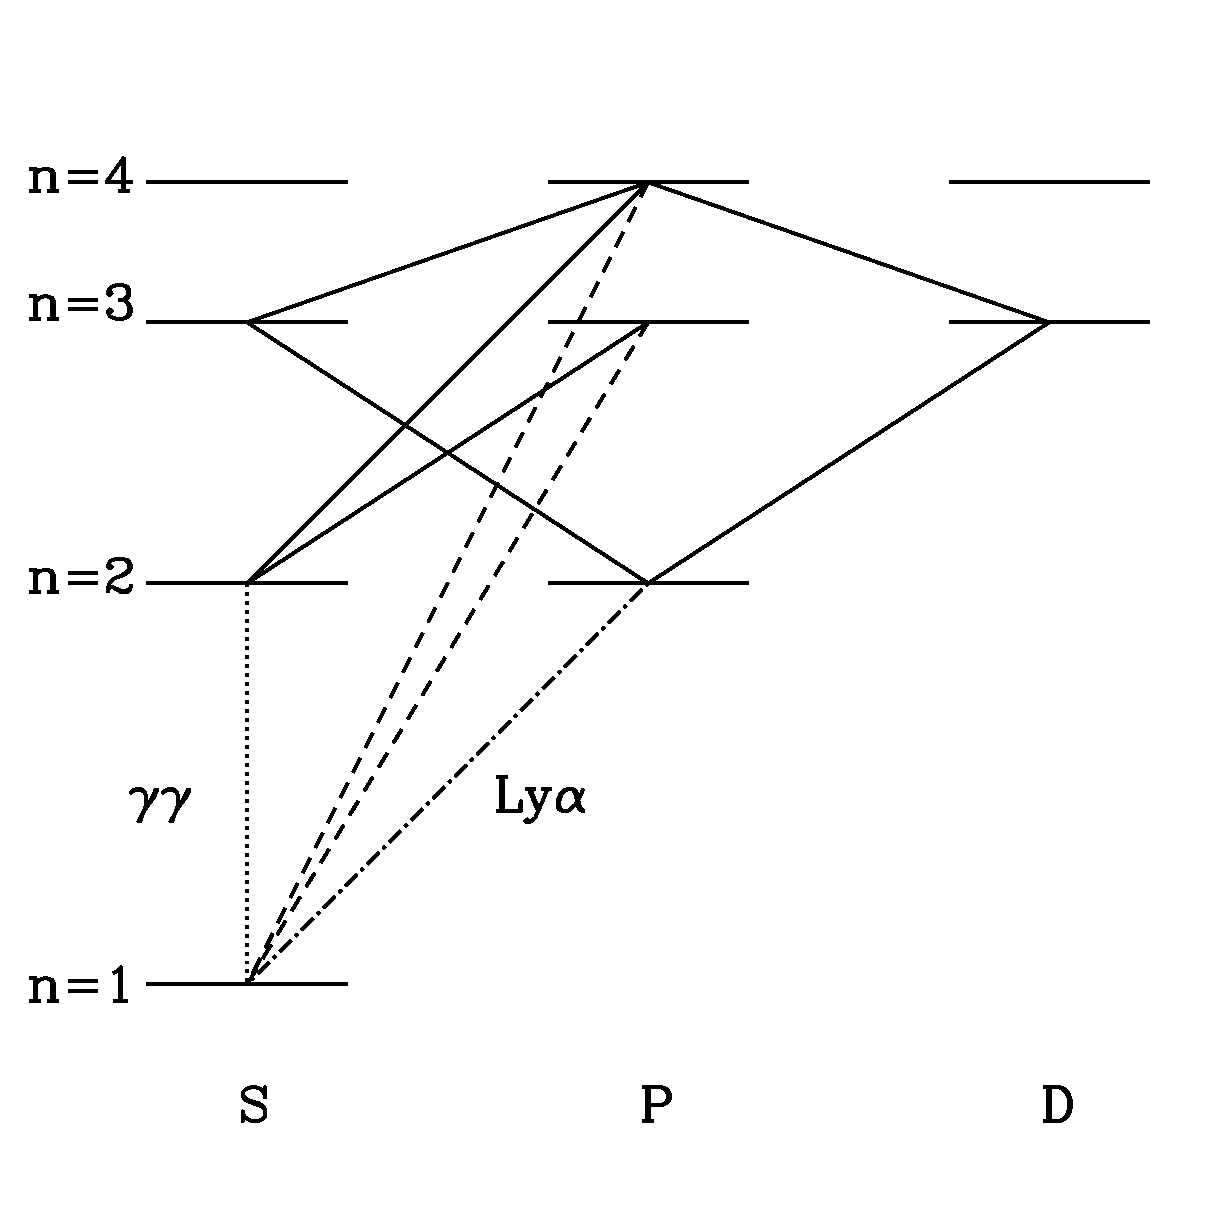
\includegraphics[width=0.6\textwidth]{Furlanetto/figure2-3}
\end{center}
\caption{Decay chains for Lyman-$\beta$ and Lyman-$\gamma$ excitations.  We show
  Lyman-$n$ transitions by dashed curves, Lyman-$\alpha$ by the dot-dashed
  curve, cascades by solid curves, and the forbidden $2S \rightarrow
  1S$ transition by the dotted curve. From \cite{pritchard06}.}
\label{fig:lygamma}
\end{figure}

The physics of the Wouthuysen-Field effect are actually much more complicated than naively expected because scattering itself modifies the shape of $J_\nu$ near the Lyman-$\alpha$ resonance \cite{chen04}. In essence, the spectrum must develop an absorption feature because of the increased scattering rate near the Lyman-$\alpha$ resonance. Photons lose energy at a fixed rate by redshifting, but each time they scatter they also lose a small amount of energy through recoil.  Momentum conservation during each scattering slightly decreases the frequency of the photon.  The strongly enhanced scattering rate near line center means that photons ``flow" through
that region more rapidly than elsewhere (where only the cosmological redshift applies), so the amplitude of the spectrum must be smaller.  Meanwhile, the scattering in such an optically thick medium also causes photons to diffuse away from line center, broadening the feature well beyond the nominal line width.

If the fractional frequency drift rate is denoted by ${\mathcal A}$, continuity requires $n_\nu {\mathcal A}=$~constant. Because ${\mathcal A}$ increases near resonance, the number density must fall.  On average, the energy loss (or gain) per scattering is \cite{chen04}
\begin{equation}
\frac{\Delta E_{\rm recoil}}{E} = \frac{h \nu}{m_p c^2} \, \left(1 - \frac{T_K}{T_c} \right),
\label{eq:recoil-loss}
\end{equation}
where the first factor comes from recoil off an isolated atom and the second factor corrects for the distribution of initial photon energies; the energy loss vanishes when $T_c = T_K$, and when $T_c < T_K$, the gas is heated by the scattering process.

To compute $S_\alpha$, we must calculate the photon spectrum near Lyman-$\alpha$.  We begin with the radiative
transfer equation in an expanding universe (written in comoving coordinates, and again using units of ~photons cm$^{-2}$ sr$^{-1}$ Hz$^{-1}$ s$^{-1}$ for $J_\nu$:
\begin{equation}
\frac{1}{c n_H \sigma_0} \, \frac{\partial J_\nu}{\partial t} = -\phi_\alpha(\nu) \, J_\nu + H \nu_\alpha \, \frac{\partial J_\nu}{\partial \nu} + \int d \nu' \, R(\nu,\nu') \, J_{\nu'} + C(t) \psi(\nu).
\label{eq:rt21}
\end{equation}
The first term on the right-hand side describes absorption, the second describes redshifting due to the Hubble flow, and the third accounts for re-emission following absorption.  $R(\nu,\nu')$ is the ``redistribution function" that specifies the frequency of an emitted photon, which depends on the relative momenta of the absorbed and
emitted photons as well as the absorbing atom. The last term accounts for the injection of new photons (via, e.g., radiative cascades that result in Lyman-$\alpha$ photons): $C$ is the rate at which they are produced and $\psi(\nu)$ is their frequency distribution.

The redistribution function $R$ is the difficult aspect of the problem, but it can be simplified if the frequency change per scattering (typically of order the absorption line width) is ``small."  In that case, we can expand $J_{\nu'}$ to second order in $(\nu-\nu')$ and rewrite equation~(\ref{eq:rt21}) as a diffusion problem in frequency.
The steady-state version of equation (\ref{eq:rt21}) becomes, in this so-called {\it Fokker-Planck} approximation, \cite{chen04}
\begin{equation}
\frac{d}{d x} \left( - {\mathcal A} \, J + {\mathcal D} \, \frac{d J}{d x} \right) + C \psi(x) = 0,
\label{eq:fokker}
\end{equation}
where $x \equiv (\nu-\nu_\alpha)/\Delta \nu_D$, $\Delta \nu_D$ is the Doppler width of the absorption profile, ${\mathcal A}$ is the frequency drift rate, and ${\mathcal D}$ is the diffusivity.  The Fokker-Planck approximation is valid so long as (i) the frequency change per scattering ($\sim \Delta \nu_D$) is smaller than the width of any spectral features, and either (iia) the photons are outside the line core where the Lyman-$\alpha$ line profile is slowly changing, or (iib) the atoms are in equilibrium with $T_c \approx T_K$.

Solving for the spectrum including scattering thus reduces to specifying ${\mathcal A}$ and ${\mathcal D}$.  The drift involves the Hubble flow, which sets ${\mathcal A}_H= - \tau_\alpha^{-1}$, where $\tau_\alpha$ is the Gunn-Peterson optical depth for the Lyman-$\alpha$ line \cite{gunn65, scheuer65}:
\begin{equation}
\tau_{\alpha} = \frac{\chi_\alpha \, n_{\rm HI}(z) \, c}{H(z) \nu_\alpha} \approx 3 \times 10^5 \, x_{\rm HI} \, \left( \frac{1+z}{7} \right)^{3/2}.
\label{eq:taugp}
\end{equation}
Because it is uniform, the Hubble flow does not introduce any diffusion. The remaining terms come from $R$ and
incorporate all the physical processes relevant to energy exchange in scattering.  The drift from recoil causes \cite{hirata06}
\begin{eqnarray}
{\mathcal D}_{\rm scatt} & = & \phi_\alpha(x)/2,
\label{eq:Dkin} \\
{\mathcal A}_{\rm scatt} & = &  -(\eta - x_0^{-1} ) \phi_\alpha(x),
\label{eq:Akin}
\end{eqnarray}
where $x_0 \equiv \nu_\alpha/\Delta \nu_D$ and $\eta \equiv (h \nu_\alpha^2)/(m_p c^2 \Delta \nu_D)$.  The latter is the recoil parameter measuring the average loss per scattering in units of the Doppler width.  The small energy defect between the hyperfine levels provides another source of slow energy exchange \cite{hirata06} and can be incorporated into the scattering in nearly the same way as recoil.

We can now solve equation~(\ref{eq:fokker}) once we choose the boundary conditions, which essentially correspond to the input photon spectrum (ignoring scattering) and the source function.  Because the
frequency range of interest is so narrow, two cases suffice: a flat input spectrum (which approximately describes photons that redshift through the Lyman-$\alpha$ resonance, regardless of the initial source spectrum)
and a step function, where photons are ``injected" at line center (through cascades or recombinations) and redshift away.  In either case, the first integral over $x$ in equation~(\ref{eq:fokker}) is trivial. At high temperatures where spin flips are unimportant to the overall energy exchange, we can write
\begin{equation}
\phi \frac{d J}{d x} + 2 \{ [\eta - (x + x_0)^{-1}] \phi + \tau_\alpha^{-1} \} J = 2 K / \tau_\alpha.
\label{eq:fokk-simp}
\end{equation}
The integration constant $K$ equals $J_\infty$, the flux far from resonance, both for photons that redshift into the line and for injected photons at $x<0$ (i.e., redward of line center); it is zero for injected photons at $x>0$.  

The formal analytic solution, when $K \neq 0$, is most compactly written in terms of $\delta_J \equiv (J_\infty -
J)/J_\infty$ \cite{chen04}:\footnote{Here we assume the gas has a sufficiently high temperature that the different hyperfine sub-transitions can be treated as one \cite{hirata06}.}
\begin{equation}
\delta_J(x) = 2 \eta \int_0^\infty d y \exp \left[ - 2 \{ \eta - (x+x_0)^{-1}\} y - {2 \over \tau_\alpha} \int_{x-y}^{x} \frac{d x'}{\phi_\alpha(x')} \right].
\label{eq:dj-soln}
\end{equation}
(An analogous form also exists for photons injected at line center.) The full problem, including the intrinsic Voigt profile of the Lyman-$\alpha$ line, must be solved numerically, but including only the Lorentzian wings from natural broadening allows a simpler solution \cite{furl06-lyheat}.  Fortunately, this assumption is quite accurate in the most interesting regime of  $T_K <  1000$~K.

%%%%%: FIGURE: Lyman-alpha spectral shape
\begin{figure}[]
\begin{center}
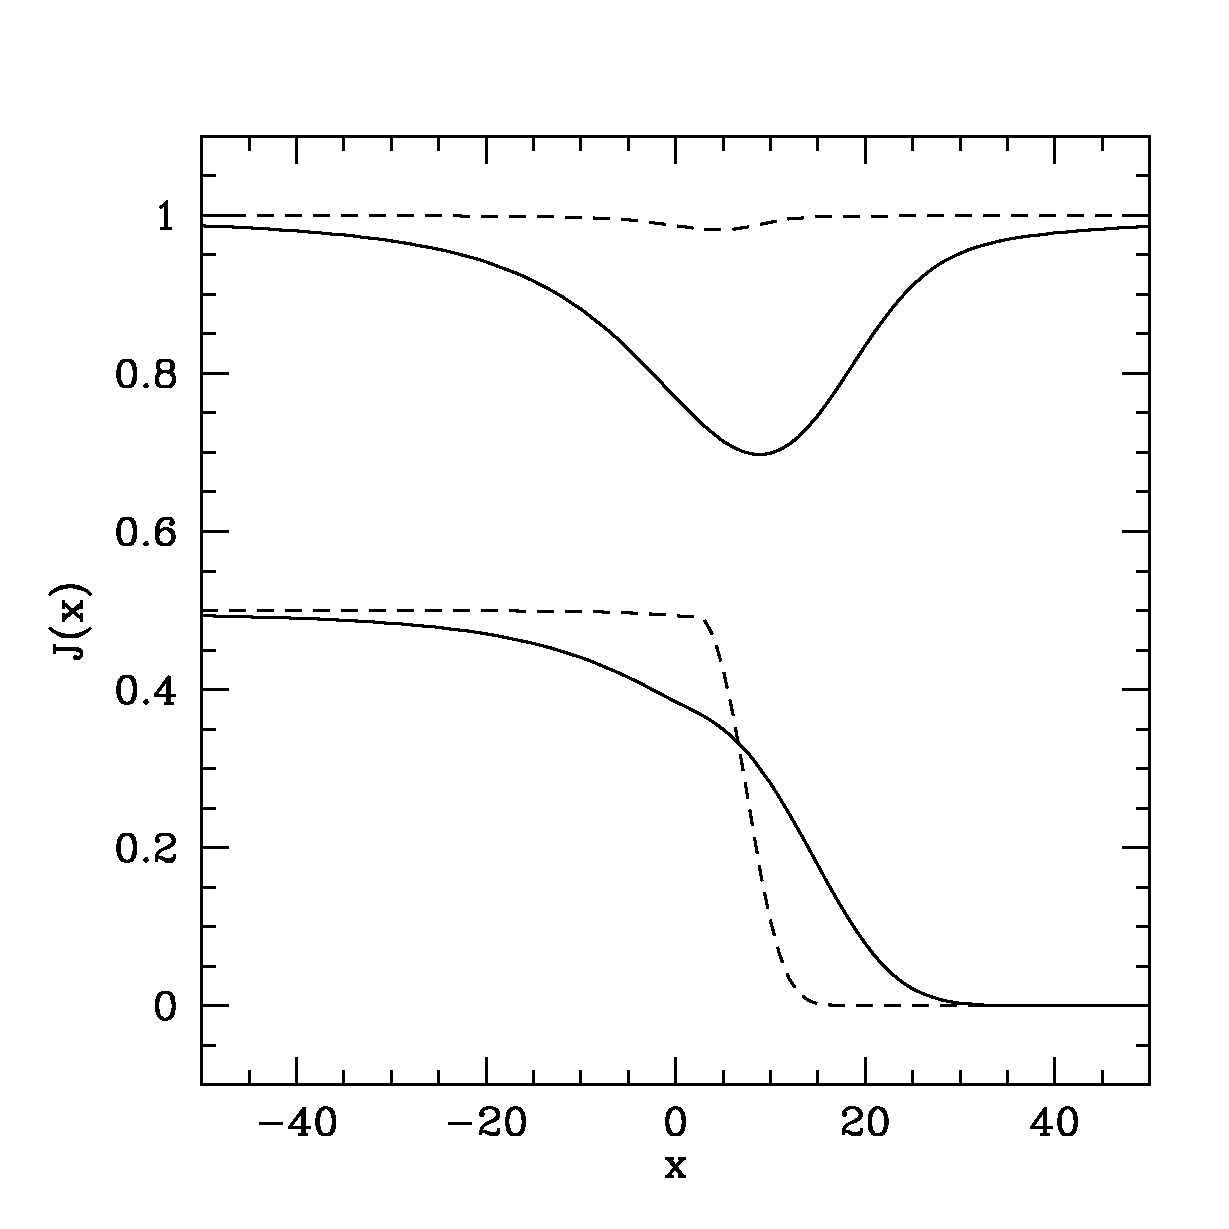
\includegraphics[width=0.6\textwidth]{Furlanetto/figure2-4}
\end{center}
\caption{Background radiation field near the Lyman-$\alpha$ resonance at $z=10$;
$x \equiv (\nu-\nu_\alpha)/\Delta \nu_D$ is the normalized deviation
from line center, in units of the Doppler width.  The upper and lower sets are for continuous photons
and photons injected at line center, respectively.  (The former are
normalized to $J_\infty$; the latter have arbitrary normalization.)
The solid and dashed curves take $T_K=10$ and $1000$~K,
respectively.  From \cite{furl06-lyheat}.}
\label{fig:lyshape}
\end{figure}

The crucial aspect of equation~(\ref{eq:dj-soln}) is that (as expected from the qualitative argument) an absorption feature appears near the line center, with its depth roughly proportional to $\eta$, our recoil parameter.  The feature is more significant when $T_K$ is small (because in that case the average effect of recoil is large). Figure~\ref{fig:lyshape} shows some example spectra (both for a continuous background and for photons injected at line center).

Usually, the most important consequence is the suppression of the radiation spectrum at line center compared to the assumed initial condition.  This decreases the total scattering rate of Lyman-$\alpha$ photons (and hence the Wouthuysen-Field coupling), with the suppression factor (defined in equation~\ref{eq:xalpha}) as \cite{chen04} 
\begin{equation}
S_\alpha = \int_{-\infty}^\infty d x \, \phi_\alpha(x)\, J(x) \approx
[1 - \delta_J(0)] \le 1,
\label{eq:salpha-defn}
\end{equation}
where the second equality follows from the narrowness of the line profile.  Again, the Lorentzian wing approximation turns out to be an excellent one; when $T_K \gg T_\star$, the suppression is \cite{furl06-lyheat}
\begin{equation} S_\alpha \sim \exp \left[ -0.803 \left({T_K\over
1~{\rm K}}\right)^{-2/3} \left( \frac{\tau_\alpha}{10^{6}}
\right)^{1/3} \right].
\label{eq:salpha-approx}
\end{equation}
Note that this form applies to both photons injected at line center as well as those that redshift in from infinity.  As we can see in Figure~\ref{fig:lyshape}, the suppression is most significant in cool gas.


\section{Heating of the Intergalactic Medium} 

We have seen that both collisions and the Wouthuysen-Field effect couple the spin temperature to the kinetic temperature of the gas. The 21-cm brightness temperature therefore depends on processes that heat the IGM. We will review several such mechanisms in this section.

\subsection{The Lyman-$\alpha$ Background} \label{sec:ch1_lya} 

The photons that trigger Lyman-$\alpha$ coupling exchange energy with the IGM, through the recoil in each scattering event. The typical energy exchange per scattering is small (see eq. \ref{eq:recoil-loss}), but the scattering rate is extremely large.  If the net heating rate per atom followed the naive expectation, $\sim
P_\alpha \times (h \nu_\alpha)^2/m_p c^2$, the kinetic temperature would surpass $T_\gamma$ soon after Wouthuysen-Field coupling becomes efficient.

However, the details of radiative transfer radically change these expectations \cite{chen04}.  In a static medium, the energy exchange \emph{must} vanish in equilibrium even though scattering continues at nearly the same rate.
Scattering induces an asymmetric absorption feature near $\nu_\alpha$ (Figure~\ref{fig:lyshape}) whose shape depends on the combined effects of atomic recoils and the scattering diffusivity.  In equilibrium, the latter exactly counterbalances the former.  

If we removed scattering, the absorption feature would redshift away as the Universe expands. Thus, the energy exchange rate from scattering must simply be that required to maintain the feature in place.  For photons redshifting into resonance, the absorption trough has total energy 
\begin{equation}
\Delta u_\alpha = (4\pi/c) \int (J_\infty - J_\nu) h \nu d \nu,
\end{equation}
where $J_\infty$ is the input spectrum, and we note that the $h \nu$ factor converts from our definition of specific intensity (which counts photons) to energy.  The radiation background loses $\epsilon_\alpha = H \Delta u_\alpha$ per
unit time through redshifting; this energy goes into heating the gas.
Relative to adiabatic cooling by the Hubble expansion, the fractional
heating amplitude is
\begin{eqnarray}
\frac{2}{3} \, \frac{\epsilon_\alpha}{k_B T_K n_H H(z) } & = & \frac{8 \pi}{3} \, \frac{h \nu_\alpha}{k_B T_K} \, \frac{J_\infty \, \Delta \nu_D}{c n_H} \, \int_{-\infty}^{\infty} d x \delta_J(x) \label{eq:epsalpha}
\\
& \approx & \frac{0.80}{T_K^{4/3}} \, \frac{x_\alpha}{S_\alpha} \left( \frac{10}{1+z} \right),
\label{eq:lyaheat}
\end{eqnarray}
Here we have evaluated the integral for the continuum photons that
redshift into the Lyman-$\alpha$ resonance; the ``injected" photons
actually cool the gas slightly.  The net energy exchange when
Wouthuysen-Field coupling becomes important (at $x_\alpha \sim
S_\alpha$) is therefore just a fraction of a degree, and in practice gas heating through Lyman-$\alpha$ scattering
is generally unimportant \cite{chen04,furl06-lyheat}.

Fundamentally, Lyman-$\alpha$ heating is inefficient because scattering diffusivity cancels the effects of recoil.  From Figure~\ref{fig:lyshape}, we see that the background spectrum is weaker on the blue side of the line than on the red.  The scattering process tends to move the photon toward line center, with the extra energy deposited in or extracted from the gas.  Because more scattering occurs on the red side, this tends to transfer energy from the gas back to the photons, mostly canceling the energy obtained through recoil.

\subsection{The Cosmic Microwave Background} 

The previous section shows that, when considered as a two-level process that acts in isolation, Lyman-$\alpha$ scattering has only a slight effect on the gas temperature. However, in reality this Lyman-$\alpha$ scattering always occurs in conjunction with scattering of CMB photons within the 21-cm transition. The combination leads to an enhanced heating rate \cite{venumadhav18}.

In essence, the process works as follows. The CMB photons scatter through the hyperfine levels of HI to heat those atoms above their expected temperature (determined in this simple case by adiabatic cooling). Meanwhile, Lyman-$\alpha$ photons scatter through the gas as well. As they do so, they mix the hyperfine levels of the HI ground state, as depicted in Figure~\ref{fig:wf} -- this is the Wouthuysen-Field effect. CMB scattering continues to heat the hyperfine level populations during the Lyman-$\alpha$ scattering, which then sweeps up this extra energy and ultimately deposits it as thermal energy through the net recoil effect.

We can estimate the energy available to this heating mechanism by considering the CMB energy reservoir \cite{venumadhav18}. The CMB energy density at the 21-cm transition is $u_\nu = (4 \pi/c) B_\nu \approx 8 \pi (\nu_{21}^2/c^3) k_B T_\gamma$. Over a redshift interval $\Delta z=1$, the total energy that redshifts through the line is $u_\nu \Delta \nu \approx 8 \pi (\nu_{21}/c)^3 k_B T_\gamma / (1+z)^2$. However, only a fraction $\tau_{10}$ actually interacts with the line. If all of this energy is used for heating, the temperature change per H atom would be
\begin{equation}
\Delta T_{\rm CMB-Ly\alpha} \approx \tau_{10} {u_\nu \Delta_\nu \over (3/2) n_H} \approx 5 x_{\rm HI} \  \left( {1 + z \over 20} \right)^{-1/2} \left( {10 \ {\rm K} \over T_S} \right) \ {\rm K}.
\label{eq:cmb-lya-heat}
\end{equation}

A more detailed calculation of the heating rate shows that it is somewhat slower, but it does amplify the effect of the Lyman-$\alpha$ heating alone by a factor of several \cite{venumadhav18}. In standard models of the early radiation backgrounds, the correction is still relatively modest, but it is not negligible. For example, in the fiducial model considered by \cite{venumadhav18}, the Lyman-$\alpha$ heating on its own modifies $T_K$ by $\sim 1$--5\%, but with the CMB scattering included the effect is $\sim 9$--15\%. Additionally, the CMB scattering can be enhanced in some exotic physics models that decrease the spin temperature substantially.

\subsection{The X-ray Background} \label{sec:ch1_xrb} 

Because they have relatively long mean free paths, X-rays from galaxies and quasars are likely to be the most important heating agent for the low-density IGM  \cite{madau97}.  In particular, photons with $E>1.5 x_{\rm HI}^{1/3} [(1+z)/10]^{1/2}$~keV have mean free paths exceeding the Hubble length \cite{oh01}.  Lower-energy X-rays will be absorbed in the IGM, depositing much of their energy as heat, as will a fraction of higher-energy X-rays.

X-rays heat the IGM gas by first photoionizing a hydrogen or helium atom.  The resulting ``primary'' electron retains most of the photon energy (aside from that required to ionize it) as kinetic energy, which it must then distribute to the general IGM through three main channels: (1) collisional ionizations, which produce more secondary electrons that themselves scatter through the IGM, (2) collisional excitations of HeI (which produce photons capable of ionizing HI) and HI (which produces a Lyman-$\alpha$ background), and (3) Coulomb collisions with free electrons (which distributes the kinetic energy .  The relative cross-sections of these processes determines what fraction of the X-ray energy goes to heating ($f_{\rm heat}$), ionization ($f_{\rm ion}$), and excitation ($f_{\rm excite}$); clearly it depends on both the ionized fraction $x_i$ and the input photon energy.  Through these scatterings, the primary photoelectrons, with $T \sim 10^6$~K, rapidly cool to energies just below the Lyman-$\alpha$ threshold, $<10$~eV, and thus equilibrate with the other IGM electrons.  After that, the electrons and neutrals equilibrate through elastic scattering on a timescale $t_{\rm eq} \sim 5 [10/(1+z)]^3$~Myr.  Because $t_{\rm eq} \ll H(z)^{-1}$, the assumption of a single temperature fluid is an excellent one.

%%%%%: FIGURE: X-ray heating
\begin{figure}[]
\begin{center}
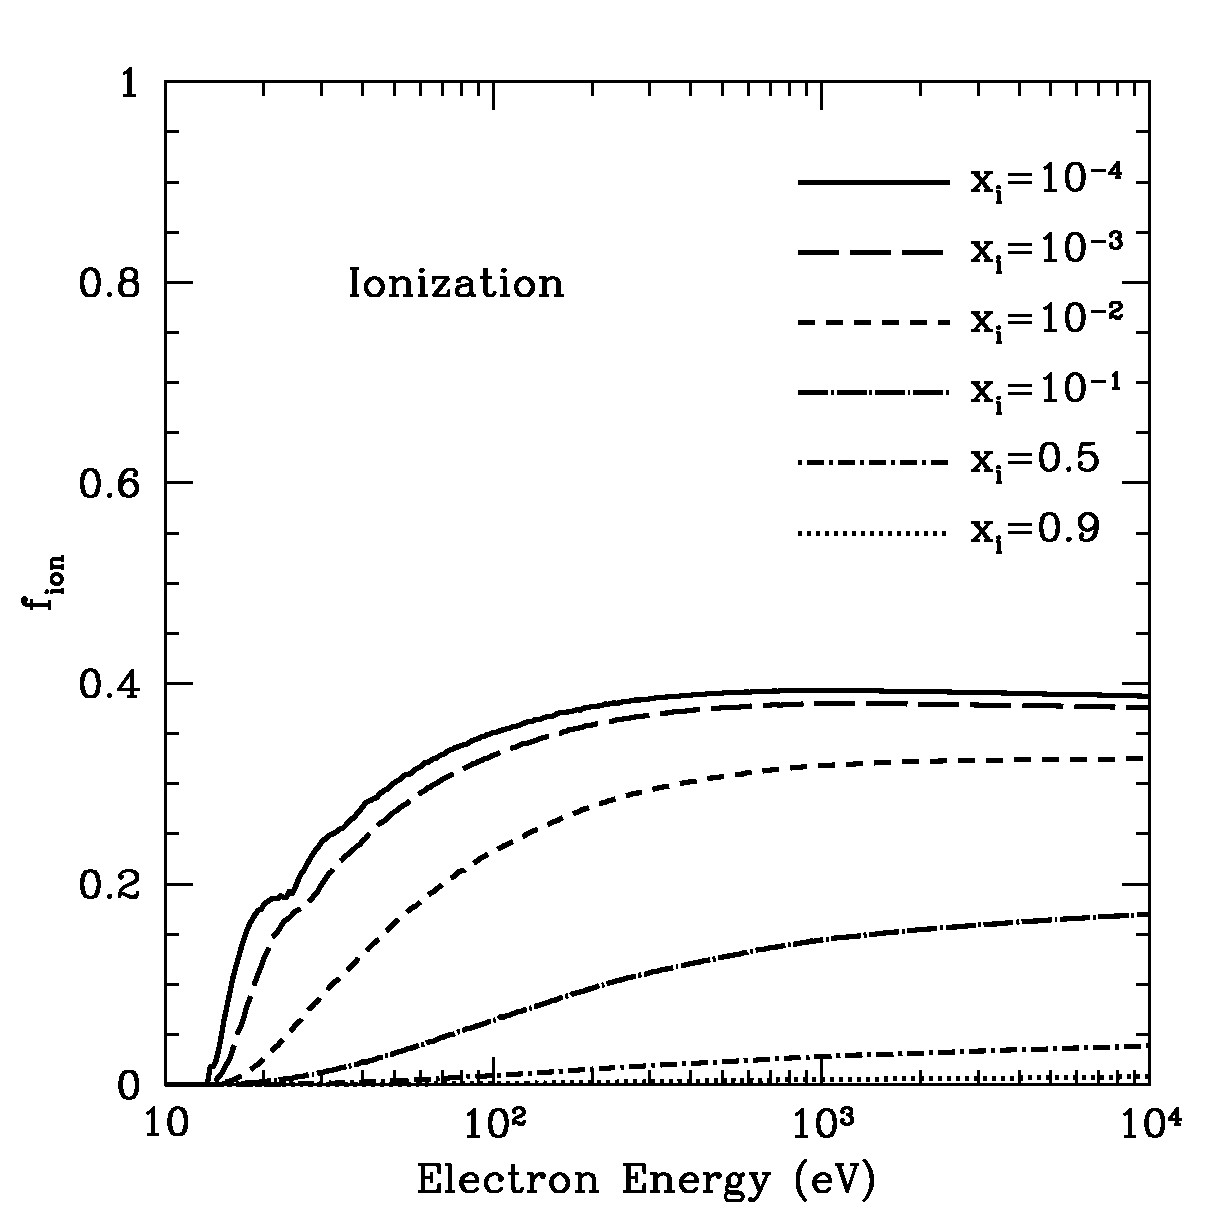
\includegraphics[width=0.4\textwidth]{Furlanetto/figure2-5a} 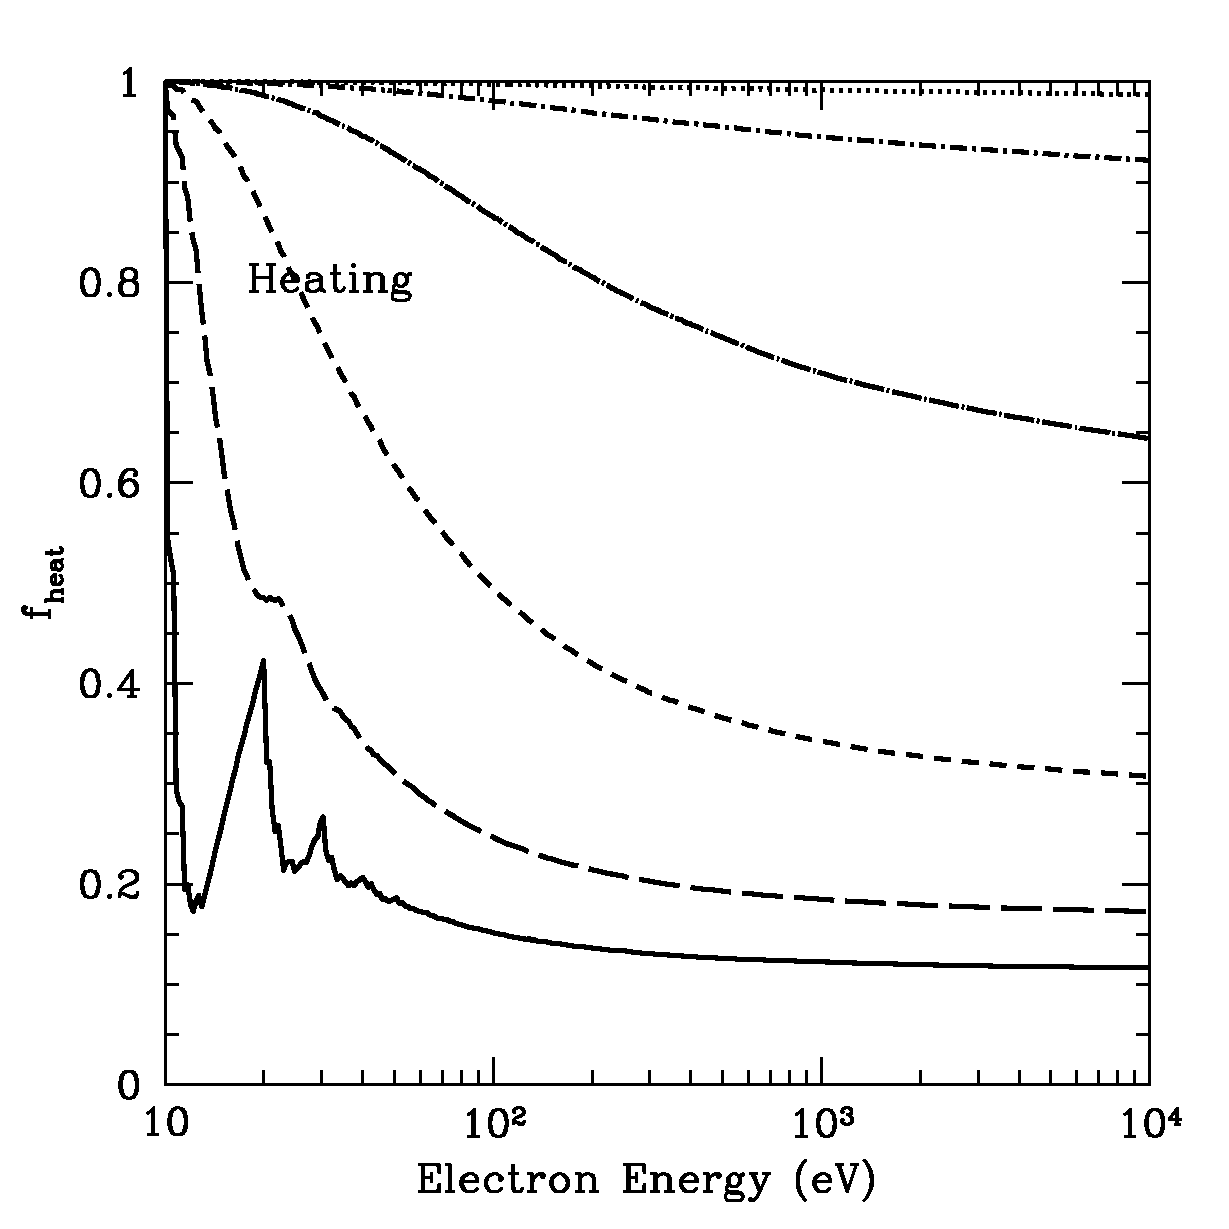
\includegraphics[width=0.4\textwidth]{Furlanetto/figure2-5b} \\
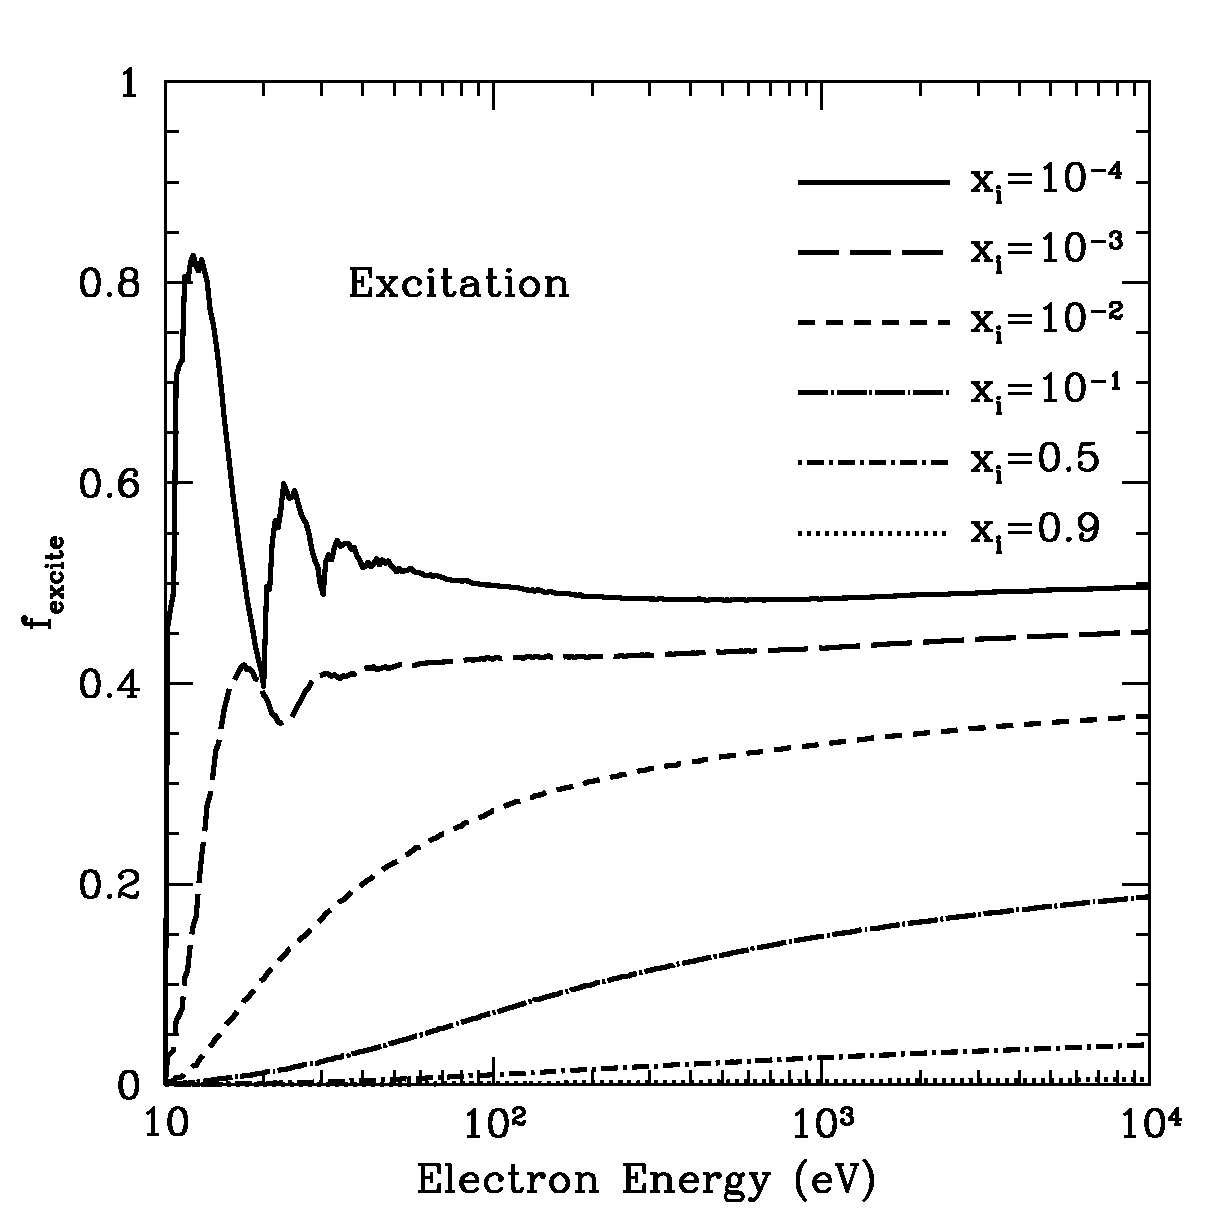
\includegraphics[width=0.4\textwidth]{Furlanetto/figure2-5c} 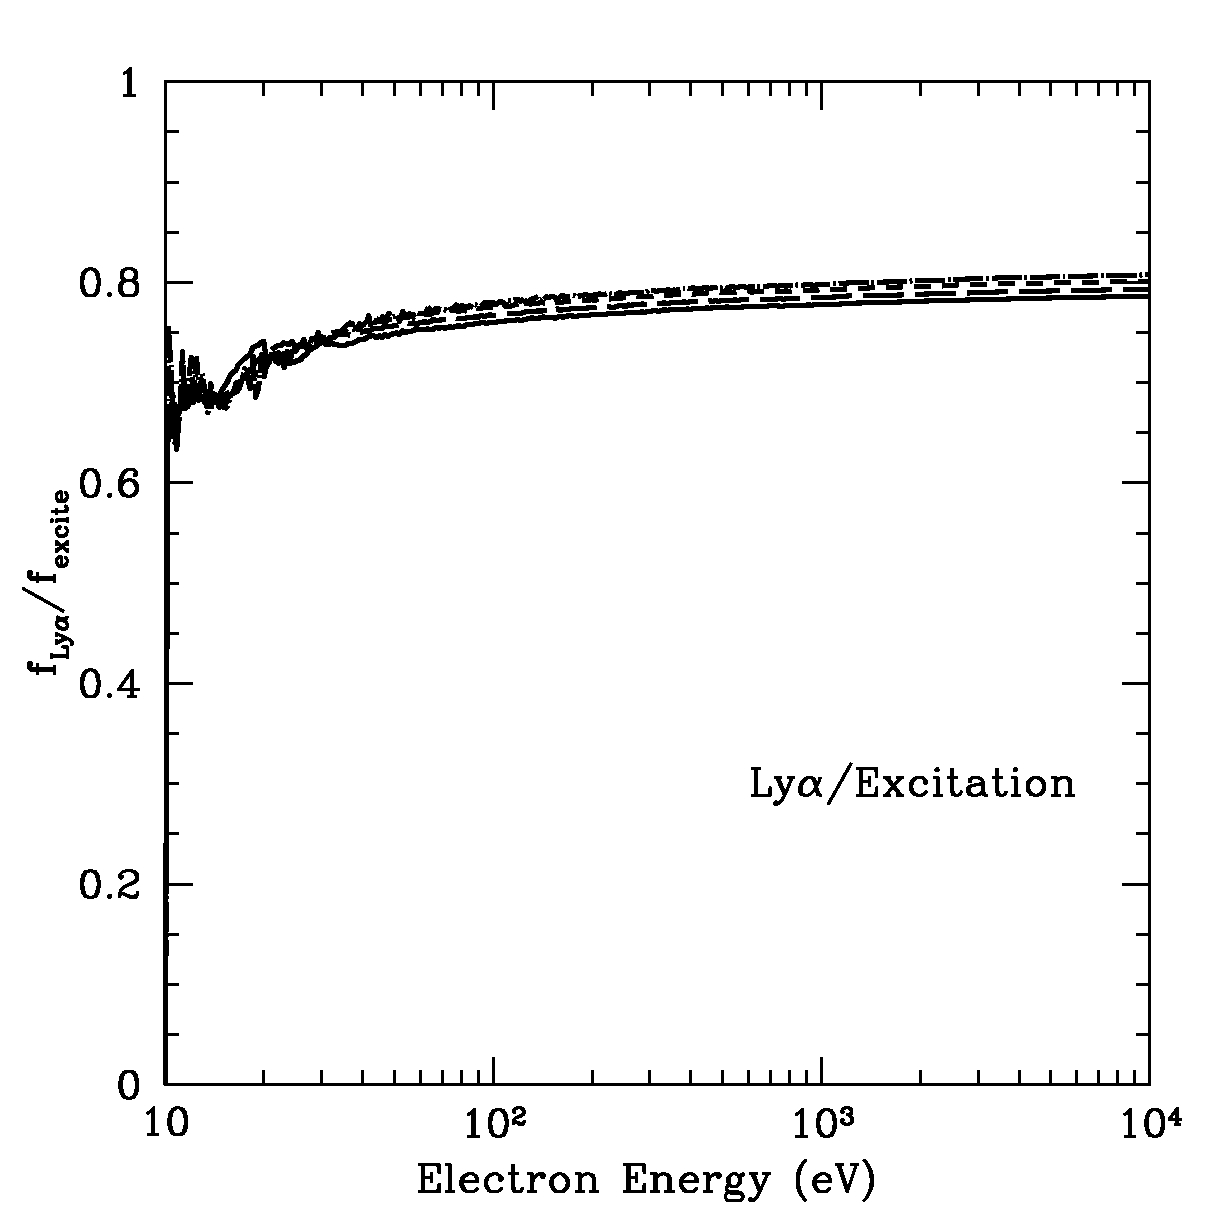
\includegraphics[width=0.4\textwidth]{Furlanetto/figure2-5d}
\end{center}
\caption{Energy deposition from fast electrons. We show the fraction of the initial energy deposited in ionization (upper left), heating (upper right), and collisional excitation (lower left), as a function of electron energy and for several different ionized fractions $x_i$. The lower right shows the fraction of the collisional excitation energy deposited in the HI Lyman-$\alpha$ transition, $f_{\rm Ly\alpha}$.  From \cite{furl10-xray}.}
\label{fig:xrayheat}
\end{figure}

The details of this process have been examined numerically \cite{shull85,valdes08,furl10-xray}, and Figure~\ref{fig:xrayheat} shows some example results. Note that the deposition fractions are smooth functions at high electron energies but, at low energies -- where the atomic energy levels become relevant -- can be quite complex. A number of approximate fits have been presented for the high-energy regime \cite{ricotti02, volonteri09}, but they are not accurate over the full energy range. A crude but useful approximation to the high-energy limit often suffices \cite{chen04-decay}:
\begin{eqnarray}
f_{\rm heat} & \sim & (1+2 x_i)/3 \nonumber \\
f_{\rm ion} \sim f_{\rm excite} & \sim & (1-x_i)/3,
\label{eq:fxapprox}
\end{eqnarray}
where $x_i$ is the ionized fraction. In highly ionized gas, collisions with free electrons dominate and $f_{\rm heat} \rightarrow 1$; in the opposite limit, the energy is split roughly equally between these three processes. However, the complexity of the behavior at low electron energies -- together with the increasing optical thickness of the IGM in that regime, and the fact that most sources are brighter in this soft X-ray regime -- suggest that a more careful treatment is needed for accurate work. \cite{furl10-xray} recommend interpolating the exact results.

\bibliographystyle{plain}
\bibliography{Furlanetto/ch2-refs}


%\newcommand*{\dt}[1]{%
  \accentset{\mbox{\large\bfseries .}}{#1}}
\newcommand*{\ddt}[1]{%
  \accentset{\mbox{\large\bfseries .\hspace{-0.25ex}.}}{#1}}

% Densities
\newcommand{\nH}{n_{\text{H}}}
\newcommand{\nHe}{n_{\text{He}}}
\newcommand{\nHbar}{\bar{n}_{\text{H}}^0}
\newcommand{\nHebar}{\bar{n}_{\text{He}}^0}
\newcommand{\nbbar}{\bar{n}_{\text{b}}^0}
\newcommand{\rhobbar}{\bar{rho}_{\text{b}}^0}

% Hydrogen and helium ions - don't add $$
\newcommand{\HI}{\text{H} {\textsc{i}}}
\newcommand{\HII}{\text{H} {\textsc{ii}}}
\newcommand{\HeI}{\text{He} {\textsc{i}}}
\newcommand{\HeII}{\text{He} {\textsc{ii}}}
\newcommand{\HeIII}{\text{He} {\textsc{iii}}}
\newcommand{\Htwo}{\text{H}_2}
\newcommand{\Hminus}{\text{H}^{-}}
\newcommand{\Hatom}{\text{H}}
\newcommand{\xibar}{\overline{x}_i}
\newcommand{\QHII}{Q_{\HII}}

\newcommand{\xipr}{x_i^{\prime}}
\newcommand{\Emin}{E_{\min}}

\newcommand{\Nion}{N_{\text{ion}}}
\newcommand{\Nlw}{N_{\text{LW}}}
\newcommand{\zetaI}{\zeta_{\text{ion}}}
\newcommand{\zetaX}{\zeta_X}
\newcommand{\zetaA}{\zeta_{\alpha}}

\newcommand{\nuLL}{\nu_{\text{LL}}}
\newcommand{\nuLya}{\nu_{\alpha}}

% Number densities of common ions
\newcommand{\nHI}{n_{\text{H } \textsc{i}}}
\newcommand{\nHII}{n_{\text{H } \textsc{ii}}}
\newcommand{\nHeI}{n_{\text{He } \textsc{i}}}
\newcommand{\nHeII}{n_{\text{He } \textsc{ii}}}
\newcommand{\nHeIII}{n_{\text{He } \textsc{iii}}}
\newcommand{\nel}{n_{\text{e}}}  
\newcommand{\ntot}{n_{\text{tot}}}

% Species fractions
\newcommand{\xHI}{x_{\text{H } \textsc{i}}}
\newcommand{\xHII}{x_{\text{H } \textsc{ii}}}
\newcommand{\xHeI}{x_{\text{He } \textsc{i}}}
\newcommand{\xHeII}{x_{\text{He } \textsc{ii}}}
\newcommand{\xHeIII}{x_{\text{He } \textsc{iii}}}

% Ionization & Recombination coefficients
\newcommand{\ionHI}{\Gamma_{\text{H } \textsc{i}}}
\newcommand{\ionHeI}{\Gamma_{\text{He } \textsc{i}}}
\newcommand{\ionHeII}{\Gamma_{\text{He } \textsc{ii}}}
\newcommand{\ionsecHI}{\gamma_{\text{H } \textsc{i}}}
\newcommand{\ionsecHeI}{\gamma_{\text{He } \textsc{i}}}
\newcommand{\ionsecHeII}{\gamma_{\text{He } \textsc{ii}}}
\newcommand{\ioncollHI}{\beta_{\text{H } \textsc{i}}}
\newcommand{\ioncollHeI}{\beta_{\text{He } \textsc{i}}}
\newcommand{\ioncollHeII}{\beta_{\text{He } \textsc{ii}}}
\newcommand{\recHII}{\alpha_{\text{H } \textsc{ii}}}
\newcommand{\recHeII}{\alpha_{\text{He } \textsc{ii}}}
\newcommand{\recHeIII}{\alpha_{\text{He } \textsc{iii}}}

\newcommand{\xiHeII}{\xi_{\text{He} \textsc{ii}}}

% Heating rate coefficients
\newcommand{\heatHI}{\mathcal{H}_{\text{H } \textsc{i}}}
\newcommand{\heatHeI}{\mathcal{H}_{\text{He } \textsc{i}}}
\newcommand{\heatHeII}{\mathcal{H}_{\text{He } \textsc{ii}}}

% Cooling rate coefficients
\newcommand{\cooldielHeII}{\omega_{\text{He } \textsc{ii}}}

% Phi and Psi
\newcommand{\PhiHI}{\Phi_{\text{H } \textsc{i}}}
\newcommand{\PhiHeI}{\Phi_{\text{He } \textsc{i}}}
\newcommand{\PhiHeII}{\Phi_{\text{He } \textsc{ii}}}
\newcommand{\PsiHI}{\Psi_{\text{H } \textsc{i}}}
\newcommand{\PsiHeI}{\Psi_{\text{He } \textsc{i}}}
\newcommand{\PsiHeII}{\Psi_{\text{He } \textsc{ii}}}

% BH stuff
\newcommand{\fduty}{f_{\text{duty}}}
\newcommand{\Cedd}{C_{\text{edd}}}
\newcommand{\tedd}{t_{\text{edd}}}
\newcommand{\Mbh}{M_{\bullet}}

\newcommand{\SFR}{\dot{M}_{\ast}}
\newcommand{\MAR}{\dot{M}_{b}}
\newcommand{\SFE}{f_{\ast}}
\newcommand{\Tmin}{T_{\min}}

% Random
\newcommand{\zprime}{z^{\prime}}
\newcommand{\dprime}{\prime\prime}
\newcommand{\fstar}{f_{\ast}}
\newcommand{\fstarbh}{\tilde{\fstar}}
\newcommand{\fbh}{f_{\bullet}}
\newcommand{\fcoll}{f_{\text{coll}}}
\newcommand{\dfcolldz}{\frac{df_{\text{coll}}}{dz}}
\newcommand{\dfcolldt}{\frac{df_{\text{coll}}}{dt}}
\newcommand{\dfcolldzbh}{\frac{d\tilde{f}_{\text{coll}}}{dz}}
\newcommand{\dfcolldtbh}{\frac{d\tilde{f}_{\text{coll}}}{dt}}
\newcommand{\mmin}{m_{\text{min}}}
\newcommand{\rhobh}{\rho_{\bullet}}
\newcommand{\rhobhdot}{\dt{\rho}_{\bullet}}
\newcommand{\rhostar}{\rho_{\ast}}
\newcommand{\rhostardot}{\dt{\rho}_{\ast}}
\newcommand{\rhostarbhdot}{\dt{\rho}_{\ast\bullet}}
\newcommand{\rhom}{\rho_m}
\newcommand{\fstardegen}{f_{\ast \bullet}}
\newcommand{\Ndot}{\dot{N}_{\text{ion}}}
\newcommand{\fesc}{f_{\text{esc}}}
\newcommand{\nmax}{n_{\text{max}}}
\newcommand{\frec}{f_{\text{rec}}}
\newcommand{\frecn}{f_{\text{rec}}^{n}}
\newcommand{\frecbar}{\overline{f}_{\text{rec}}}
\newcommand{\Msun}{M_{\odot}}

\newcommand{\SFRunits}{M_{\odot} \ \text{s}^{-1}}
\newcommand{\fbin}{f_{\text{bin}}}
\newcommand{\fact}{f_{\text{act}}}
\newcommand{\fsurv}{f_{\text{surv}}}

\newcommand{\JLW}{J_{\text{LW}}}

\newcommand{\fion}{f_{\text{ion}}}
\newcommand{\nnu}{$n_{\nu}$}
\newcommand{\ncol}{N_i}
\newcommand{\Tvir}{T_{\text{vir}}}

\newcommand{\NHI}{N_{H\textsc{i}}}


\newcommand{\emissivity}{\text{erg} \ \text{s}^{-1} \ \text{Hz}^{-1} \ \text{cMpc}^{-3}}

\newcommand{\Ja}{J_{\alpha}}
\newcommand{\Lya}{\text{Ly-}\alpha}
\newcommand{\Lyn}{\text{Ly-}n}
\newcommand{\TS}{T_{\text{S}}}
\newcommand{\TK}{T_{\text{K}}}
\newcommand{\Tcmb}{T_{\text{CMB}}}
\newcommand{\TCMB}{T_{\text{CMB}}}
\newcommand{\TR}{T_{\text{R}}}

% Physical constants
\newcommand{\kB}{k_{\text{B}}}

\newcommand{\esc}{\text{esc}}

% Overlap regions
\newcommand{\IV}{\mathcal{V}}
\newcommand{\OV}{\mathcal{O}}
\newcommand{\pos}{\mathbf{x}}
\newcommand{\pospr}{\mathbf{x}^{\prime}}
\newcommand{\xpr}{x^{\prime}}

\newcommand{\fheat}{f^{\text{heat}}}
\newcommand{\fXh}{f_{X,h}}
\newcommand{\fioni}{f_i^{\text{ion}}}
\newcommand{\Lbol}{\mathcal{L}_{\text{bol}}}
\newcommand{\spec}{\mathcal{N}}
\newcommand{\Heat}{\mathcal{H}}
\newcommand{\trec}{$t_{\text{rec}}$}
\newcommand{\Lbox}{L_{\mathrm{box}}}
\newcommand{\dx}{\Delta x}
\newcommand{\dd}{\text{d}}

\newcommand{\drIF}{$\Delta r_{\mathrm{IF}}$}
\newcommand{\dTb}{$\delta T_b$}
\newcommand{\Nvec}{\mathbf{N}}
\newcommand{\sh}{\mathrm{sh}}
\newcommand{\Mdot}{\dot{M}}
\newcommand{\Ledd}{L_{\text{edd}}}
\newcommand{\intensityunits}{\text{erg} \ \text{s}^{-1} \ \text{cm}^{-2} \ \mathrm{Hz}^{-1} \ \text{sr}^{-1}}
\newcommand{\intensityunitsnumber}{\text{s}^{-1} \ \text{cm}^{-2} \ \mathrm{Hz}^{-1} \ \text{sr}^{-1}}


\chapter{Astrophysics from the 21-cm background}

\begin{bf}
  \author{Jordan Mirocha}\\
\\
\end{bf}

The goal of this chapter is to describe the astrophysics encoded by the 21-cm background. We will begin in \S\ref{sec:RT} with a general introduction to radiative transfer and ionization chemistry in gas of primordial composition. Then, in \S\ref{sec:techniques}, we will introduce techniques used to model the the UV and X-ray backgrounds that drive re-ionization and re-heating of the intergalactic medium (IGM). In \S\ref{sec:sources}, we will provide a review of the most plausible sources of ionization and heating in the early Universe, and in \S\ref{sec:predictions}, we will summarize the status of current 21-cm predictions, build some intuition for how different model parameters affect the observable signals, and highlight the modeling tools available today.



%Figures 
%\begin{itemize}
%	\item Picture of reionization simulation.
%	\item Schematic of ray tracing
%	\item Show 1-D profiles to build intuition?
%	\item Show mean ionization and temperature histories from published work, defer on details of modeling assumptions to later sections.
%	\item Stellar spectra
%	\item XRB spectra 
%	\item Empirical constraints on $L_X$-SFR.
%\end{itemize}
%
%
%Here's my approach:
%\begin{itemize}
%	\item Talk about how 21-cm traces ionization and heating. Outline generic non-Eq chemistry setup and how one would do this in ``all its glory.''
%	\item Motivate separation of ionization and heating (mean free path), and how that allows more approximate techniques and useful conceptual framework. Outline those approximate techniques.
%	\item Turn to the sources. We've discussed how to model ionization and heating but not what the source terms are. Focus on evolution of individual sources and source populations (i.e., frequency bit then redshift/R bit)
%	\item Put it all together: basic predictions. Intuition for timing of different features in global signal and power spectrum, prospects for breaking degeneracies between different sources/parameters. Discussion of available tools, differences, progress? Lump in with previous section.
%\end{itemize}


%%%
%% Ionization, thermal, and Ly-a histories
%%%
\section{Properties of the High-$z$ Intergalactic Medium} \label{sec:RT}
In this section we provide a general introduction to the intergalactic medium (IGM) and how its properties are expected to evolve with time. We will start with a brief recap of the 21-cm brightness temperature (\ref{sec:dTb}), then turn our attention to its primary dependencies, the ionization state and temperature of the IGM, and the radiative processes relevant to their evolution on scales large and small (\S\ref{sec:ioniz_heating}). Readers familiar with the basic physics may skip ahead to \S\ref{sec:techniques}, in which we focus specifically on how this physics is incorporated in 21-cm modeling codes.

% T_21
\subsection{The brightness temperature} \label{sec:dTb}
The differential brightness temperature\footnote{Can replace this first sub-section with pointers to Chapter 1 to avoid redundancy.} of a patch of the IGM at redshift $z$ and position $\mathbf{x}$ is given by\footnote{Refer back to Chapter 1 for a more detailed introduction.} 
\begin{equation}
    \delta T_b(z, \mathbf{x}) \simeq 27 (1 + \delta) (1 - x_i) \left(\frac{\Omega_{b,0} h^2}{0.023} \right) \left(\frac{0.15}{\Omega_{m,0} h^2} \frac{1 + z}{10} \right)^{1/2} \left(1 - \frac{T_R}{T_S} \right) , \label{eq:dTb}
\end{equation}
where $\delta$ is the baryonic overdensity relative to the cosmic mean, $x_i$ is the ionized fraction, $T_R$ is the radiation background temperature (generally the CMB, $T_R = T_{\gamma}$), and
\begin{equation}
    T_S^{-1} \approx \frac{T_R^{-1} + x_c T_K^{-1} + x_{\alpha} T_{\alpha}^{-1}}{1 + x_c + x_{\alpha}} . \label{eq:Ts}
\end{equation}
is the spin temperature, which quantifies the level populations in the ground state of the hydrogen atom, and itself depends on the kinetic temperature, $T_K$, and ``colour temperature'' of the Lyman-$\alpha$ radiation background, $T_{\alpha}$. Because the IGM is optically thick to Ly-$\alpha$ photons, the approximation $T_K \approx T_{\alpha}$ is generally very accurate.

The collisional coupling coefficients, $x_c$, themselves depend on the gas density, ionization state, and temperature, and were computed as a function of temperature in \cite{Zygelman2005}. The radiative coupling coefficient, $x_{\alpha}$, depends on the Ly-$\alpha$ intensity, $J_{\alpha}$, via
\begin{equation}
    x_{\alpha} = \frac{S_{\alpha}}{1+z} \frac{\hat{J}_{\alpha}}{{J}_{\alpha,0}} \label{eq:xalpha}
\end{equation}
where
\begin{equation}
    J_{\alpha,0} \equiv \frac{16\pi^2 T_{\star} e^2 f_{\alpha}}{27 A_{10} T_{\gamma,0} m_e c} . \label{eq:Jnorm}
\end{equation}
$\hat{J}_{\alpha}$ is the angle-averaged intensity of Ly-$\alpha$ photons in
units of $\intensityunitsnumber$, $S_{\alpha}$ is a correction factor that
accounts for variations in the background intensity near line-center
\cite{Chen2004,FurlanettoPritchard2006,Hirata2006}, $m_e$ and $e$ are the
electron mass and charge, respectively, $f_{\alpha}$ is the $\Lya$ oscillator
strength, $T_{\gamma,0}$ is the CMB temperature today, and $A_{10}$ is the Einstein A coefficient for the 21-cm transition.

A more detailed introduction to collisional and radiative coupling can be found in Chapter 1. For the purposes of this chapter, the key takeaway from Equations \ref{eq:dTb}-\ref{eq:xalpha} is simply that the 21-cm background probes the ionization field, kinetic temperature field, and $\Lya$ background intensity. We quickly review the basics of non-equilibrium ionization chemistry in the next sub-section (\S\ref{sec:ioniz_heating}) before moving on to techniques used to model these properties of the IGM in \S\ref{sec:techniques}.


% Global signal
%\subsubsection{The ``global'' 21-cm signal}
%On very large scales...
%\begin{align}
%    \delta T_b \simeq 27 (1 - \mathbf{x_i}) \left(\frac{\Omega_{b,0} h^2}{0.023} \right) \left(\frac{0.15}{\Omega_{m,0} h^2} \frac{1 + z}{10} \right)^{1/2} \left(1 - \frac{T_R}{T_S} \right) , \label{eq:dTb}
%\end{align}
%
%Many experiments are targeting this signal. For this reason, modeling efforts for the global signal often take an approximate approach. Under the assumption that fluctuations in $\delta$, $x_i$, and $T_S$ are uncorrelated, the volume-averaged differential brightness temperature is simply related to the volume-averaged density, ionization fraction, and spin temperature. Averaging over large volumes means $\delta \approx 0$, and while in general these fields \textit{will} be correlated, {\color{red} the effects are likely minor: cite that one paper that Xueli Chen is on.}
%
%
%In the next three sections, we walk through the main epochs of evolution relevant to the 21-cm background, starting with reionization, and working our way backwards in time to first light. As in this section, boldfaced symbols refer to variables with an implicit spatial dependence, while regularly typset symbols refer to the spatial average. {\color{red} is this too tedious?}
%
%Talk here about how in numerical simulations we would just do radiative transfer so there's no need to break up all these things. But, RT is expensive, so in practice most models (at least those used for inference) make approximations, and it is very convenient to consider

%%
% RT background?
%%
\subsection{Basics of Non-Equilibrium Ionization Chemistry} \label{sec:ioniz_heating}
As described in the previous section, the 21-cm brightness temperature of a patch of the IGM depends on the ionization and thermal state of the gas, as well as the incident Ly-$\alpha$ intensity\footnote{Note that Ly-$\alpha$ photons can transfer energy to the gas though we omit this dependence from the current discussion (see \S\ref{sec:ch1_lya}).}. The evolution of the ionization and temperature are coupled and so must be evolved self-consistently. The number density of hydrogen and helium ions in a static medium can be written as the following set of coupled differential equations:
\begin{align}
    \frac{d \nHII}{dt} & = (\ionHI + \ionsecHI + \ioncollHI \nel) \nHI - \recHII \nel \nHII   \label{eq:HIIRateEquation} \\
    \frac{d \nHeII}{dt} & = (\ionHeI + \ionsecHeI + \ioncollHeI \nel) \nHeI \nonumber + \recHeIII \nel \nHeIII  - (\ioncollHeII + \recHeII + \xiHeII) \nel \nHeII \\ & - (\ionHeII + \ionsecHeII) \nHeII \label{eq:HeIIRateEquation} \\ 
    \frac{d \nHeIII}{dt} & = (\ionHeII + \ionsecHeII + \ioncollHeII \nel) \nHeII  - \recHeIII \nel \nHeIII . \label{eq:HeIIIRateEquation} .
\end{align}
Each of these equations represents the balance between ionizations of species
\HI, \HeI, and \HeII, and recombinations of \HII, \HeII, and
\HeIII. Associating the index $i$ with absorbing species, $i = $\HI, \HeI,
\HeII, and the index $i^{\prime}$ with ions, $i^{\prime} = $\HII, \HeII,
\HeIII, we define $\Gamma_i$ as the photo-ionization rate coefficient,
$\gamma_i$ as the rate coefficient for ionization by photo-electrons \cite[and \S\ref{sec:ch1_xrb}]{Shull1985,Furlanetto2010}, $\alpha_{i^{\prime}}$
($\xi_{i^{\prime}}$) as the case-B (dielectric) recombination rate
coefficients, $\beta_i$ as the collisional ionization rate coefficients, and
$\nel = \nHII + \nHeII + 2\nHeIII$ as the number density of electrons.

While the coefficients $\alpha$, $\beta$, and $\xi$ only depend on the gas temperature, the photo- and secondary-ionization coefficients, $\Gamma$ and $\gamma$, depend on input from astrophysical sources and thus constitute much of the challenge for theoretical models. We will revisit these coefficients in more detail momentarily.

The final equation necessary in a primordial chemical network is that governing the kinetic temperature evolution, which we can write as a sum of various heating and cooling processes, i.e.,
\begin{align}
    \frac{3}{2}\frac{d}{dt}\left(\frac{\kB T_k \ntot}{\mu}\right) & = \fheat  \sum_i n_i \Lambda_i - \sum_i \zeta_i \nel n_i - \sum_{i^{\prime}} \eta_{i^{\prime}} \nel n_{i^{\prime}} \nonumber \\ & - \sum_i \psi_i \nel n_i - \cooldielHeII \nel \nHeII \label{eq:TemperatureEvolution} .
\end{align}
Here, $\Lambda_i$ is the photo-electric heating rate coefficient (due to
electrons previously bound to species $i$), $\cooldielHeII$ is the dielectric
recombination cooling coefficient, and $\zeta_i$, $\eta_{i^{\prime}}$, and
$\psi_i$ are the collisional ionization, recombination, and collisional
excitation cooling coefficients, respectively, where primed indices
$i^{\prime}$ indicate ions $\HII$, $\HeII$, and $\HeIII$, and unprimed
indices $i$ indicate neutrals $\HI$, $\HeI$, and $\HeII$. The constants in
Equation (\ref{eq:TemperatureEvolution}) are the total number density of
baryons, $\ntot = n_\mathrm{H} + n_{\mathrm{He}} + \nel$, the mean molecular
weight, $\mu$, Boltzmann's constant, $\kB$, and the fraction of photo-electron energy deposited as heat, $\fheat$ \cite{Shull1985,Furlanetto2010}. Formulae to compute the values of
$\alpha_i$, $\beta_i$, $\xi_i$, $\zeta_i$, $\eta_{i^{\prime}}$, $\psi_i$, and
$\cooldielHeII$, are compiled in, e.g., \cite{Fukugita1994,Hui1997}.

These equations do not yet explicitly take into account the cosmic expansion, which dilutes the density and adds an adiabatic cooling term to Eq. \ref{eq:TemperatureEvolution}, however these generalizations are straightforward to implement in practice, as we will show in the next section. For the duration of this chapter we will operate within this simple chemical network, ignoring, e.g., molecular species like $\Htwo$ and $\mathrm{HD}$ whose cooling channels are important in primordial gases. Though an interesting topic in their own right, molecular processes reside in the ``subgrid'' component of most 21-cm models, given that they influence how, when, and where stars are able to form (see \S\ref{sec:sources}), but do not directly affect the bulk properties of the IGM on large scales to which 21-cm measurements are sensitive. 

%%
% POINT SOURCES
%%
\subsection{Ionization and Heating Around Point Sources} \label{sec:smallscales}
In order to build intuition for the progression of ionization and heating in the IGM it is instructive to consider the impact of a single point source of UV and X-ray photons on its surroundings. Many early works focused on such 1-D radiative transfer problems \cite{Iliev2006,Thomas2008}. In principle, this is the ideal way to simulation reionization -- iterating over all sources in a cosmological volume and for each one applying 1-D radiative transfer techniques over the surrounding $4\pi$ steradians. In practice, such approaches are computationally expensive, and while they provide detailed predictions \cite{OShea2015,Ocvirk2016,Gnedin2014}, more approximate techniques are required to survey the parameter space and perform inference (see Chapter 3).

In 1-D, the change in the intensity of a ray of photons, $I_{\nu}$, is a function of the path length, $s$, the emissivity of sources along the path, $j_{\nu}$, and the absorption coefficient, $\alpha_{\nu}$, 
\begin{equation}
	dI_{\nu} = j_{\nu} - \alpha_{\nu} I_{\nu} .
\end{equation}
If considering a point source, $j_{\nu} = 0$, we can integrate to obtain
\begin{equation}
	I_{\nu}(s) = I_{\nu,0} \exp\left[-\int_0^s \alpha_{\nu}(s^{\prime}) ds^{\prime} \right] ,
\end{equation}
i.e., the intensity of photons declines exponentially along the ray. It is customary to define the optical depth, $\tau_{\nu}$, as
\begin{equation}
	d\tau_{\nu} = \alpha_{\nu} ds ,
\end{equation}
in which case we can write
\begin{equation}
	I_{\nu}(s) = I_{\nu,0} e^{-\tau_{\nu}} .
\end{equation}
In the reionization context, the optical depth of interest is that of the IGM, which is composed of (almost) entirely hydrogen and helium\footnote{Note that metals on small scales will also contribute some opacity, though in most models it is galaxies themselves that are the point sources of radiation from which we solve the RTE, rather than individual sources within galaxies. As a result,  one's choice of source spectrum should encode any intrinsic attenuation from metals (or H and He) in the interstellar medium. See \S\ref{sec:sources} for more details.}, in which case the optical depth is 
\begin{equation}
	\tau_{\nu} = \sum_i \sigma_{\nu,i} N_i
\end{equation}
where $i=\HI,\HeI,\HeII$, and $N_i = \int_0^s ds^{\prime} n_i(s^{\prime})$ is the column density of each species along the ray.

With a solution for $I_{\nu}(s)$ in hand, one can determine the photoionization and heating rates by integrating over all photon frequencies and weighting by the bound-free absorption cross section for each species. For example, the photoionization rate coefficient for hydrogen is given by
\begin{equation}
	\Gamma_{\HI}(s) = \int_{\nu_{\HI}}^{\infty} \sigma_{\HI} I_{\nu}(s) \frac{d\nu}{h\nu} \label{eq:GammaHI}
\end{equation}
where $\nu_{\HI}$ is the frequency of the hydrogen ionization threshold, $h\nu=13.6$ eV.

Note that in practice the RTE is solved on a grid, in which case it may be difficult to achieve high enough spatial resolution to ensure photon conservation. For example, a discretized version of Eq. \ref{eq:GammaHI} uses the intensity of radiation incident upon the face of a resolution element to calculate the photoionization rate within that element, but the radiation incident on the subsequent resolution element is not guaranteed correctly reflect the attenuation within the preceding element. As a result, in order to guarantee photon conservation, it is common to slightly reframe the calculation as follows \cite{Abel1999}:
\begin{align}
    \Gamma_i & = A_i \int_{\nu_i}^{\infty} I_{\nu} e^{-\tau_{\nu}} \left(1 - e^{-\Delta \tau_{i,\nu}}\right) \frac{d\nu}{h\nu} \label{eq:PhotoIonizationRate} \\
    \gamma_{ij} & = A_j \int_{\nu_j}^{\infty} \left(\frac{\nu - \nu_j}{\nu_i}\right) I_{\nu} e^{-\tau_{\nu}} \left(1 - e^{-\Delta \tau_{j,\nu}}\right) \frac{d\nu}{h\nu} \label{eq:SecondaryIonizationRate} \\
    \Lambda_i & = A_i \int_{\nu_i}^{\infty} (\nu - \nu_i) I_{\nu} e^{-\tau_{\nu}} \left(1 - e^{-\Delta \tau_{i,\nu}}\right) \frac{d\nu}{\nu}  \label{eq:HeatingRate} .
\end{align}
The normalization constant in each expression is defined as $A_i \equiv L_{\mathrm{bol}}/n_i V_{\sh}(r)$, where $V_{\sh}$ is the volume of a shell in this 1-D grid of concentric spherical shells, each having thickness $\Delta r$ and volume $V_{\sh}(r) = 4 \pi [(r + \Delta r)^3 - r^3] / 3$, where $r$ is the distance between the origin and the inner interface of each shell. We denote the ionization threshold energy for species $i$ as $h\nu_i$. $I_{\nu}$ represents the SED of radiation sources, and satisfies $\int_{\nu} I_{\nu} d\nu = 1$, such that $L_{\mathrm{bol}} I_{\nu} = L_{\nu}$. Note that the total secondary ionization rate for a given species is the sum of ionizations due to the secondary electrons from all species, i.e., $\gamma_i = \fion \sum_j \gamma_{ij} n_j / n_i$.

These expressions preserve photon number by inferring the number of photo-ionizations of species $i$ in a shell from the radiation incident upon it and its optical depth \cite{Abel1999},
\begin{equation}
    \Delta \tau_{i,\nu} = n_i \sigma_{i,\nu} \Delta r .
\end{equation}    
This quantity is not to be confused with the total optical depth between source and shell, $\tau_{\nu} = \tau_{\nu}(r)$, which sets the incident radiation field upon each shell, i.e.,
\begin{align}
    \tau_{\nu}(r) & = \sum_i \int_0^r \sigma_{i,\nu} n_i(r^{\prime}) dr^{\prime} \nonumber \\
                  & = \sum_i \sigma_{i,\nu} \ncol(r) \label{eq:OpticalDepth}
\end{align}
where $\ncol$ is the column density of species $i$ at distance $r$ from the
source. 

In words, Equations \ref{eq:PhotoIonizationRate}-\ref{eq:HeatingRate} are propagating photons from a source at the origin, with bolometric luminosity $L_{\mathrm{bol}}$, and tracking the attenuation suffered between the source and some volume element of interest at radius $r$, $e^{-\tau}$, and the attenuation within that volume element, $\Delta \tau$, which results in ionization and heating. In each case, we integrate over the contribution from photons at all frequencies above the ionization threshold, additionally modifying the integrands for $\gamma_{ij}$ and $\Lambda_i$ with $(\nu - \nu_i)$-like factors to account for the fact that both the number of photo-electrons (proportional to $(\nu - \nu_j) / \nu_i$) and their energy (proportional to $\nu - \nu_i$) determine the extent of secondary ionization and photo-electric heating. 

Equations \ref{eq:PhotoIonizationRate}-\ref{eq:HeatingRate} can be solved once a source luminosity, $L_{\mathrm{bol}}$, spectral shape, $I_{\nu}$, and density profile of the surrounding medium, $n(r)$, have been specified. In practice, to avoid performing these integrals on each step of an ODE solver (for Eqs. \ref{eq:HIIRateEquation}-\ref{eq:TemperatureEvolution}), the results can be tabulated as a function of $\tau$ or column density, $N_i$, where $\tau_{i,\nu}=\sigma_{i,\nu} N_i$ \cite{Thomas2008,Mirocha2012}.

%\begin{figure*}[]
%\begin{center}
%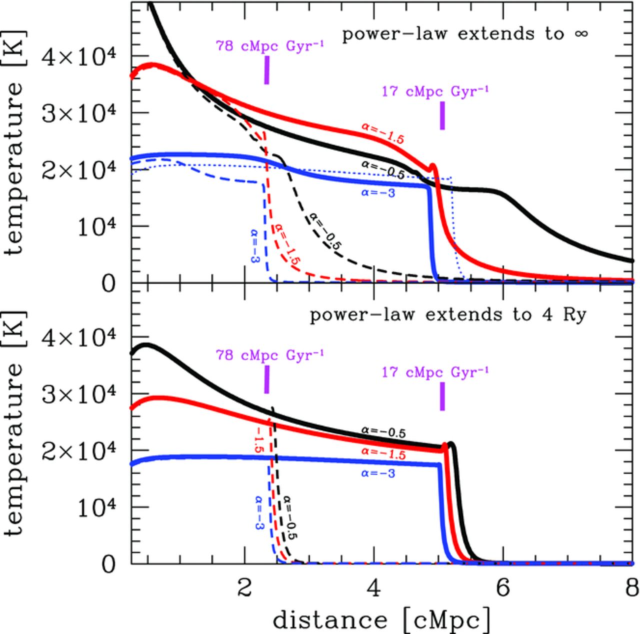
\includegraphics[width=0.98\textwidth]{Mirocha/mcquinn2012_fig5.pdf}
%\end{center}
%\caption{{\bf Temperature profile around power-law sources in an expanding IGM \cite{McQuinn2012}. \textit{Right:} \cite{Knevitt2014}}}
%\label{fig:fzh04}
%\end{figure*}

\begin{figure*}[]
\begin{center}
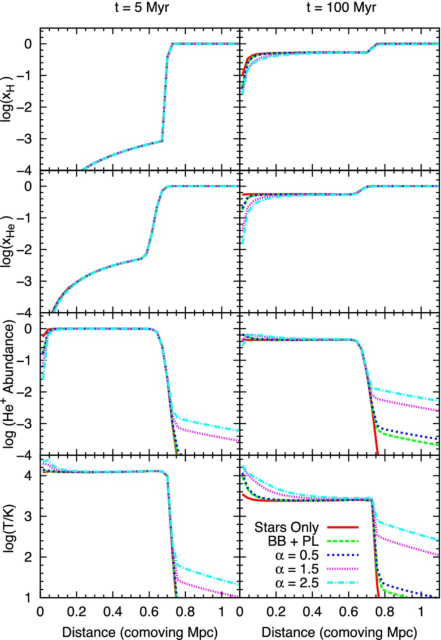
\includegraphics[width=0.98\textwidth]{Mirocha/knevitt2014_fig3.pdf}
\end{center}
\caption{{\bf Ionization and temperature profile around stellar UV and X-ray sources \cite{Knevitt2014}.}}
\label{fig:fzh04}
\end{figure*}

{\color{red} Motivate photon counting approach used in semi-analytic/numeric models.}


%%
% Metagalactic background
%%
\subsection{Ionization and Heating on Large Scales} \label{sec:largescales}
While the procedure outlined in the previous section is relevant to small-scale ionization and heating, i.e., that which is driven a single (or perhaps a few) source(s) close to a volume element of interest, it is also instructive to consider the ionization and heating caused by a \textit{population} of sources separated by great distances. In this limit, rather than considering the luminosity of a single source at the origin of a 1-D grid, we treat the volume-averaged emissivity of sources, $\epsilon_{\nu}$, in a large ``chunk'' of the Universe, and solve for the evolution of the mean intensity in this volume, $J_{\nu}$.

The transfer equation now takes its cosmological form, i.e., 
\begin{equation}
    \left(\frac{\partial}{\partial t} - \nu H(z) \frac{\partial}{\partial \nu} \right) J_{\nu}(z) + 3 H(z) J_{\nu}(z) =  \frac{c}{4\pi} \epsilon_{\nu}(z) (1 + z)^3 - c \alpha_{\nu} J_{\nu}(z) \label{eq:rte_diffeq}
\end{equation}
where $J_{\nu}$ is the mean intensity in units of $\intensityunits$, $\nu$ is the observed frequency of a photon at redshift $z$, related to the emission frequency, $\nu^{\prime}$, of a photon emitted at redshift $z^{\prime}$ as
\begin{equation}
    \nu^{\prime} = \nu \left(\frac{1 + z^{\prime}}{1 + z}\right) , \label{eq:EmissionFrequency}
\end{equation}
$\alpha_{\nu} = n \sigma_{\nu}$ is the absorption coefficient, not to be confused with recombination rate coefficient, $\alpha_{\HII}$, and $\epsilon_{\nu}$ is the co-moving emissivity of sources.

The optical depth, $d\tau = \alpha_{\nu} ds$, experienced by a photon at redshift $z$ and emitted at $z^{\prime}$ is a sum over absorbing species,
\begin{equation}
    \overline{\tau}_{\nu}(z, z^{\prime}) = \sum_j \int_{z}^{z^{\prime}} n_j(z^{\dprime}) \sigma_{j, \nu^{\dprime}} \frac{dl}{dz^{\dprime}}dz^{\dprime} \label{eq:tau_igm}
\end{equation}
In general, one must iteratively solve for $\overline{\tau}_{\nu}$ and $J_{\nu}$. However, in many models the bulk of cosmic re-heating precedes reionization, in which case $\overline{\tau}_{\nu}$ can be tabulated assuming a fully neutral IGM. This approach provides a considerable speed-up computationally and remains accurate even when reionization and reheating partially overlap \cite{Mirocha2014}.

The solution to Equation \ref{eq:rte_diffeq} {\color{red} assuming X, Y, and Z} is
\begin{equation}
    \hat{J}_{\nu} (z) = \frac{c}{4\pi} (1 + z)^2 \int_{z}^{z_f} \frac{\epsilon_{\nu}^{\prime}(z^{\prime})}{H(z^{\prime})} e^{-\overline{\tau}_{\nu}} dz^{\prime} . \label{eq:AngleAveragedFlux}
\end{equation}    
where $z_f$ is the ``first light redshift'' when astrophysical sources first turn on, $H$ is the Hubble parameter, and the other variables take on their usual meaning. This equation can be solved efficiently on a logarithmic grid in $x\equiv 1+z$ \cite{Haardt1996,Mirocha2014}, in which case photons redshift seamlessly between frequency bins over time.

With the background intensity in hand, one can compute the rate coefficients for ionization and heating. These coefficients are equivalent to those for the 1-D problem (Eqs. \ref{eq:PhotoIonizationRate}-\ref{eq:HeatingRate}), though the intensity of radiation at some distance $R$ from the source has been replaced by the mean background intensity,
\begin{align}
    \Gamma_{i}(z) & = 4 \pi n_i(z) \int_{\nu_{\min}}^{\nu_{\max}} \hat{J}_{\nu} \sigma_{\nu,i} d\nu  \\
    \gamma_{ij}(z) & = 4 \pi \sum_j n_j \int_{\nu_{\min}}^{\nu_{\max}}  \hat{J}_{\nu} \sigma_{\nu,j} (h\nu - h\nu_j) \frac{d\nu}{h\nu}  \\
    \epsilon_X(z) & = 4 \pi \sum_j n_j \int_{\nu_{\min}}^{\nu_{\max}}  \hat{J}_{\nu}  \sigma_{\nu,j} (h\nu - h\nu_j) d\nu
\end{align}
Then, the ionization state and temperature of the gas can be updated accordingly via Equations \ref{eq:HIIRateEquation}-\ref{eq:TemperatureEvolution}.

{\color{red} Show figure for mean ionization and temperature evolution.}

%%%
%% EVOLUTION EQUATIONS. I. Ionization
%%%
\section{Techniques for Modeling the IGM} \label{sec:techniques}
In the previous section we introduced the basics of ionization chemistry and radiative transfer in a primordial medium and explored extreme limits on very small and very large scales. These limits bracket the range of possibilities for volume elements, which are subject to radiation from a single (or few) source(s) nearby or the combined radiative output of many sources at cosmological distincances. Reality is often somewhere between, which poses a challenge for numerical models of reionization.  

In order to roughly identify the transition between these extremes, it is useful to consider the mean free path of photons in a hydrogen-only medium \cite{McQuinn2012},
\begin{equation}
	\lambda_{\HI} \approx 7 \xHI^{-1} \left(\frac{h\nu}{200 \ \mathrm{eV}} \right)^{2.6} \left(\frac{1+z}{10} \right)^{-2} \ \mathrm{cMpc} \label{eq:mfp},
\end{equation}
i.e., mean-free paths for UV photons with $h\nu \ll 0.2$ keV are very short. Because of this, the IGM is divided roughly into two different phases: (i) a fully-ionized phase composed of ``bubbles,'' which grow around UV sources, and (ii) a ``bulk IGM'' phase outside bubbles in which ionization and heating is dominated by X-rays. The boundaries between these two phases can become fuzzy if reionization is driven by sources with hard spectra. However, even in such cases, the two-phase picture is a useful conceptual framework for understanding evolution in the 21-cm background, and provides a basis for approximations to the radiative transfer that have enabled the development of more efficient reionization models.

In this section, we describe the evolution of the ionization and temperature fields in this two-zone framework, in each case focusing first on the volume-averaged evolution relevant to the global 21-cm signal, and then the spatial structure relevant for 21-cm fluctuations. Because there are a variety of modeling approaches outlined in the literature, here we try only to convey the basic flavor of 21-cm models, as well as the advantages and disadvantages of various techniques. Note also that for now, we will not specify the properties of UV and X-ray sources, but instead fold their properties into a single time-, frequency-, and position-dependent emissivity, $\epsilon = \epsilon_{\nu}(z,R)$. Models for $\epsilon$ will be put forth in \S\ref{sec:sources}, from which 21-cm predictions will follow in \S\ref{sec:predictions}. 

%Hydrogen atoms can be ionized by photons with energies $h\nu > 13.6$ eV. The bound-free cross-section for interaction between photons and hydrogen atoms in the ground state is given approximately by\footnote{See \cite{Verner1996} for more detailed fits to the cross section as a function of photon energy.}
%\begin{equation}
%	\sigma_{\HI} \simeq 6 \times 10^{18} \left(\frac{h\nu}{13.6 \ \mathrm{eV}} \right)^{-3} \ \mathrm{cm}^{-2} . \label{eq:xsec}
%\end{equation}	
%In a hydrogen-only medium, the mean free path is (e.g., \cite{McQuinn2012})
%\begin{equation}
%	l \equiv \frac{1}{n_{\HI} \sigma_{\HI}} \simeq 100 \ \mathrm{kpc} \left( \frac{0.0486}{\Omega_{b,0} h^2} \right) \left(\frac{0.9187}{1-y}\right) \left( \frac{E}{13.6 \mathrm{eV}} \right)^3 \left(\frac{10}{1+z} \right)^3 \label{eq:mfp}
%\end{equation}


%%
% DENSITY
%%
\subsection{The Density Field}
\subsubsection{Global Evolution} \label{sec:density_global}
Equation \ref{eq:dTb} casts the differential brightness temperature as a function of the baryon overdensity relative to the cosmic mean, i.e., $\delta = 0$ refers to gas at the cosmic mean density. It is common in simple models of the global 21-cm signal to neglect correlations between the density, ionization, and spin temperature, and simply set $\delta = 0$. In general the product of the averages is \textit{not} equal the average of the product, but in practice there is at least qualitative agreement between purely global 21-cm models (in which $\delta = 0$) and more sophisticated models with realistic density fields. 

\subsubsection{Spatial Structure} \label{sec:density_local}
Briefly introduce the halo model \cite{Cooray2002} and \textsc{DexM}.

%%
% IONIZATION FIELD
%%
\subsection{The Ionization Field}

% Global ionization evolution
\subsubsection{Global Evolution} \label{sec:ionization_global}
In the two phase approximation of the IGM, the volume-averaged ionized fraction is a weighted average between the fully-ionized phase, with volume filling fraction $\QHII$, and the (likely) low-level ionization in the bulk IGM phase, characterized by its electron fraction, $x_e$, i.e.,
\begin{equation}
	\xibar = \QHII + (1 - \QHII) x_e
\end{equation}
In the limit of neglible ionization in the bulk IGM phase, $\xibar \approx \QHII$, we recover the standard ionization balance equation for reionization,
\begin{equation}
	\frac{d \QHII}{dt} = \nHI \Gamma_{\HI} - n_e \nHII \alpha_{\HII} . \label{eq:ion_balance}
\end{equation}
%where we have written the rate coefficient for photo-ionization generically as {\color{red} the ionization photon production rate}...We have also neglected collisional ionization and ionization by hot photo-electrons, though such effects could be absorbed into $\Gamma_{\HI}$\footnote{Secondary ionization is generally unimportant in HII regions since stars do not emit much above 1 Rydberg. As a result, photo-electrons are incapable of causing further ionization, and instead deposit most of their energy in heat or collisional excitation.}.

%The recombination coefficient is a function of temperature,
%\begin{equation}
%	\alpha_{\HII} = 2.6 \times 10^{-13} \left(\frac{T_K}{10^4 \ \mathrm{K}} \right)^{-0.8}
%\end{equation}

%Note: unlike the post-EoR Universe, we never really care about the UV background because it only exists inside bubbles. Up until late times, the background intensity in bubbles cannot reasonably be considered a useful global metric since it only traces galaxies relatively nearby (i.e., in that bubble).

The mean ionization history is currently only crudely constrained. High-$z$ quasar spectra suggest that reionization ended at $z \sim 6$ but provide no information on the detailed history. The CMB optical depth provides an integral constraint on reionization, i.e.,
\begin{equation}
	\tau_e = \int_0^{R_{\mathrm{ls}}} ds n_e (s) \sigma_T
\end{equation}
where $\sigma_T = 6.65 \times 10^{-25} \ \mathrm{cm}^{-2}$ is the Thomson cross section, and $R_{\mathrm{ls}}$ is the distance to the last scattering surface, and thus only roughly constrains the timing and duration of reionization. Figure \ref{fig:mason2018} shows a recent compilation of constraints on the mean reionization history \cite{Mason2018} compared to the predictions of semi-empirical models (see \S\ref{sec:sfe}). 

\begin{figure}[]
\begin{center}
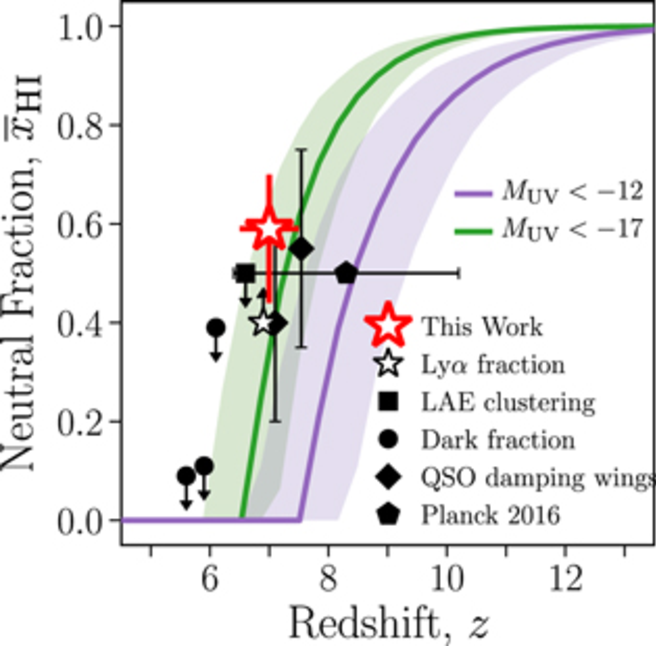
\includegraphics[width=0.5\textwidth]{Mirocha/mason2018_fig12.pdf} 
\end{center}
\caption{{\bf Current constraints on the mean ionization history \cite{Mason2018}.}}
\label{fig:fzh04}
\end{figure}

In principle there is much more information in the spatial fluctuations in the ionization field, simple models for which we discuss in the next section.



% Spatial structure of ionization field
\subsubsection{Spatial Structure} \label{sec:ionization_local}
While the evolution of the average ionized fraction contains a wealth of information about the properties of UV (and perhaps X-ray) sources in the early Universe, fluctuations in the ionization field contain much more information. Indeed, the patchy ``swiss cheese'' structure generic to UV-driven reionization scenarios provided the initial impetus to study reionization via 21-cm interferometry \cite{Madau1997}.

If computational resources were no issue, radiative transfer simulations would be the ideal tool to approach this problem for reasons that will be apparent momentarily. However, once again, the two-phase approximation opens the door to a simple statistical treatment of fluctuations in the ionization field. Given that 21-cm fluctuation efforts are geared largely toward measuring the 21-cm power spectrum, here we restrict our discussion to the ionization power spectrum, which forms a part of the 21-cm power spectrum that we will describe in more detail in \S\ref{sec:predictions}. We will follow closely the early work of \cite{Furlanetto2004} in what follows.

The power spectrum of the ionization field is simply the Fourier transform of its two-point correlation function, which we can write as
\begin{equation}
	\xi \equiv \langle x_i x_i^{\prime} \rangle - \langle x_i \rangle^2 ,
\end{equation}
where $x_i$ is the ionized fraction at a point $\mathbf{p}$, while $x_i^{\prime}$ is the ionized fraction at a point $\mathbf{p}^{\prime} = \mathbf{p} + \mathbf{R}$, i.e., a different point a distance $\mathbf{R}$ from the first point. The expectation value is related to the joint probability, i.e.,
\begin{equation}
	\langle x_i \xipr \rangle = \int dx_i \int d\xipr x_i \xipr f(x_i, \xipr) .
\end{equation}
If we now assume that ionization in the ``bulk'' IGM is negligible, $x_i$ is a binary field, taking on values of 0 or 1 exclusively. In this limit, the expectation value is simply
\begin{equation}
	\langle x_i \xipr \rangle = f(x_i=1, \xipr=1) \equiv P_{ii} ,
\end{equation}
i.e., $\langle x_i \xipr \rangle$ is equivalent to the probability that both points are ionized. 

Now, to model the probability of ionization we first assume that the ionizatoin field is composed of discrete, spherical bubbles, with size distribution $dn/dR$. Then, taking inspiration from the halo model \cite{Cooray2002}, we can write $P_{ii}$ as the sum of two terms,
\begin{equation}
	P_{ii} = P_{ii,1b} + P_{ii,2b}
\end{equation}
where the first term encodes the probability that both points are within a single bubble (hence the ``1b'' subscript), while the second term is the probability that points are in two different bubbles. 

Two points separated by $r_{12}$ can be ionized by the same bubble so long as the diameter of the bubble is the distance between the points or greater. For bubbles bigger than the absolute minimum ($r_{12}$), there is an ``overlap region,'' with volume $\IV$, in which a bubble of mass $m$ can ionize both points.

If $p_1$ is ionized, then the probability that $p_2$ is ionized by the same source will be equal to the probability that a sufficiently large source, with mass $m$, resides within the overlap region of $p_1$ and $p_2$, whose volume depends on their separation. The overlap region, $V_o$, is thus given by the area of intersection between two spheres, assumed here to have the same radius $R$, placed a distance $r_{12}$ apart,
\begin{equation}
  \IV = 
  \begin{cases}
    \frac{4}{3}\pi R(m)^2 - \pi r_{12} \left[R(m)^2 - \frac{r_{12}^2}{12} \right] & r_{12} \leq 2 R(m) \\
    0 & r_{12} > 2 R(m)
  \end{cases}
  \label{eq:V_overlap}
\end{equation}
We will denote the probability that two points are ionized by a source of mass $m$ as $P\left[m,\IV(m,r_{12})\right]$.

This argument results in an infinite sum over probabilities, with each successive terms corresponding to the probability that a point is ionized by increasingly large bubbles (accounting for the probability that smaller bubbles could \textit{not} ionize both points, i.e., the product of the negation of all previous terms), i.e.,
\begin{align}
    P_{ii,1} (r_{12}) & = P\left[m_1,\IV(m_1,r_{12})\right] \nonumber \\
    & + (1 - P\left[m_1,\IV(m_1,r_{12})\right]) P\left[m_2,\IV(m_2,r_{12})\right] + ... \nonumber \\
    %& = P_1 + (1 - P_1) P_2 + (1 - P_1)(1 - P_2) P_3 + ... \nonumber \\
    %& = P_1 + (P_2 - P_1 P_2) + (P_3 - P_3 P_1 - P_3 P_2 + P_1 P_2 P_3) + ... \nonumber \\
    %& = 1 - P_1 P_2 - (P_1 P_3 - P_2 P_3 + P_1 P_2 P_3) + ... \nonumber \\
    %& = 1 - (1 - P_1) (1  - P_2) (1 - P_3) ... \nonumber  \\
    %& = 1 - \Pi_i (1 - P_i) \nonumber \\
    & = 1 - \exp \left[ \sum_i \log(1 - P_i) \right]
\end{align}
To compute the probabilities, we need only the abundance of sources as a function of their mass, which we will leave as a general quantity, $n(m)$, for now, and the overlap volume, i.e.,
\begin{equation}
    P\left[m_1,\IV(m_1,r_{12})\right] = n(m_1) \IV(m_1,r_{12})
\end{equation}
The final step is to realize that $P_i = 1 - \exp\left[-n_i V_i] \right]$, which follows from a Poissonian argument, i.e., assuming that
\begin{equation}
    P_i = \frac{\lambda^N e^{-\lambda}}{N!} .
\end{equation}
However, we are uninterested in exactly how many sources ionize a point -- we care only about whether the point is ionized -- so we need only compute the probability that there's \textit{not} a source in the volume, and subtract that from unity to obtain the probability that there's \textit{any kind of} source in the volume. We know the mean number of bubbles, so we can make a Poissonian argument with $N=0$ to determine this probability, i.e.,
\begin{equation}
    P(N \geq 1) = 1 - P(N = 0) = 1 - e^{-\lambda} \label{eq:P1src}
\end{equation}
So, the probability that two points like in a single ionized bubble is
\begin{equation}
    P_{ii,1} (r_{12}) = 1 - \exp \left[ -\sum_i n(m_i) \IV(m_i,r_{12}) \right]
\end{equation}
The other possibility is that two points are members of two different bubbles, which we denote with the probability $P_{ii,2}$. The probability of this occurring is the probability that a single source \textit{cannot} ionize both points, times the probability that a source of mass $m$ is able to ionize the first point but not the second. If we visualize the overlap of two spheres, we need the second source \textit{not} to reside in the overlap region. So, we can simply replace $\IV \rightarrow V(m) - \IV$ in Equation \ref{eq:P1src}, and square it (to obtain probability of two sources). The total probability is then
\begin{align}
    \langle x \xpr \rangle & = P_{ii,1} + P_{ii,2} \nonumber \\
    & = 1 - \exp \left[- \int n(m) \IV(m,r_{12}) dm \right] \nonumber \\
    & + \exp \left[- \int n(m) \IV(m,r_{12}) dm \right] \times \left\{1 - \exp \left[- \int n(m) (V(m) - \IV(m,r_{12})) dm \right] \right\}^2
\end{align}
This is only valid if we neglect clustering of sources. In reality, if we're in the neighborhood of a bubble, there's a good chance there's another bubble nearby. So, we can replace one of the terms in curly braces with $n(m) \rightarrow n(m) (1 + \xi_{bb}(m, r_{12}))$, where $\xi_{bb}$ is the excess probability of finding a bubble of mass $m$ a distance $r_{12}$ away from another bubble.

At this point, it is clear that the ``bubble size distribution'', or equivalent bubble mass distribution, $n(m)$, of sources will determine the nature of the ionization field. {\color{red} Very quickly summarize the results of the excursion set approach and defer to references here. Point to \S\ref{sec:codes} for a discussion of how codes do this in practice.}

\begin{figure}[]
\begin{center}
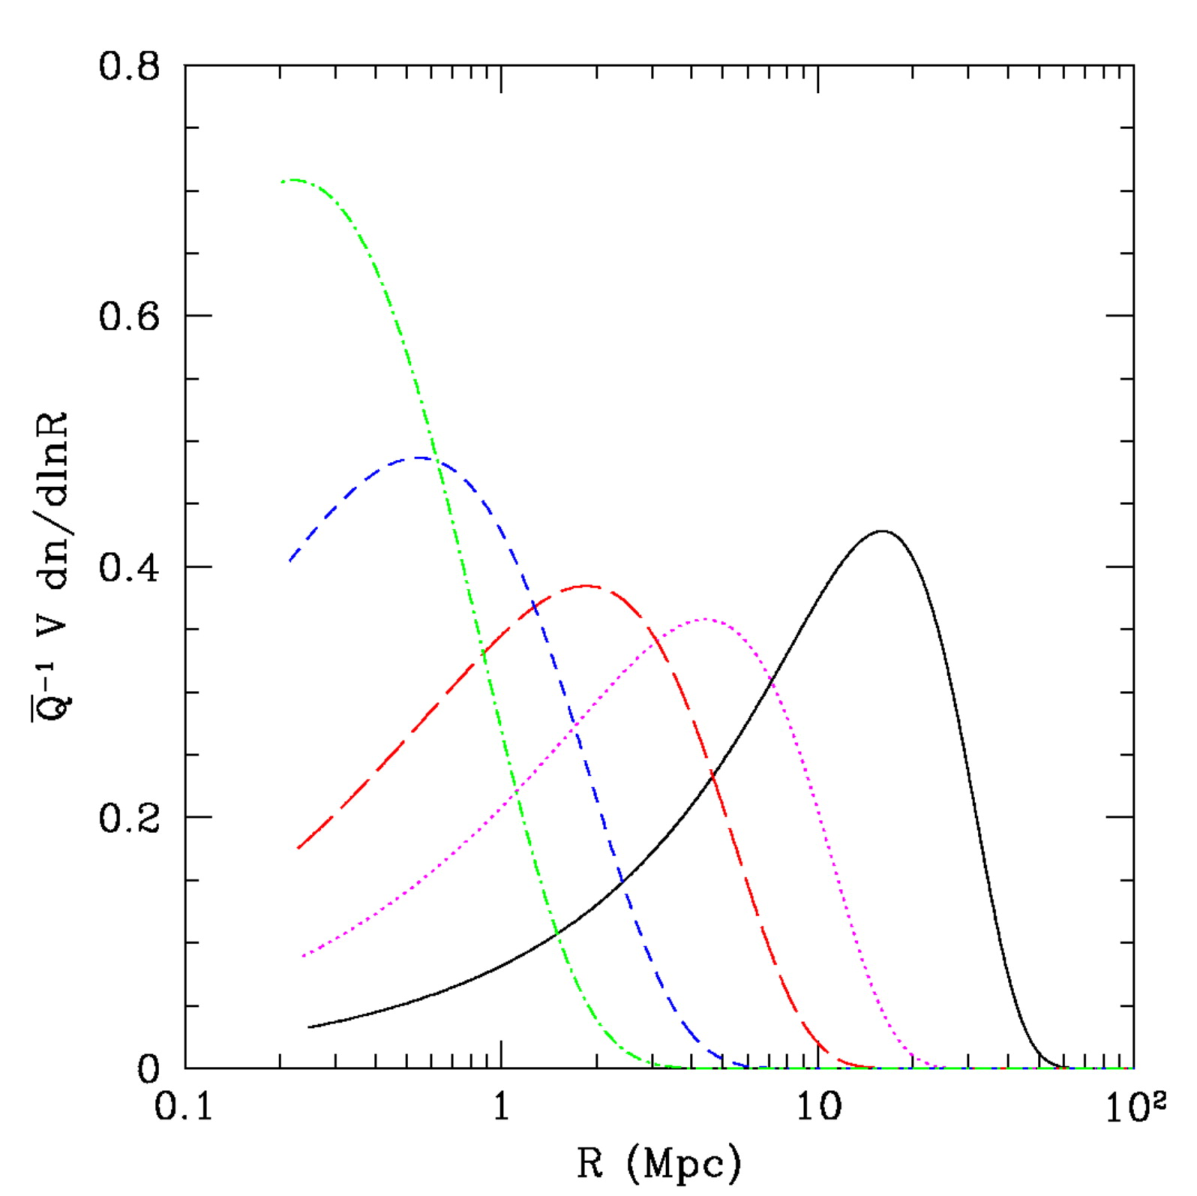
\includegraphics[width=0.3\textwidth]{Mirocha/fzh04_fig2.pdf} 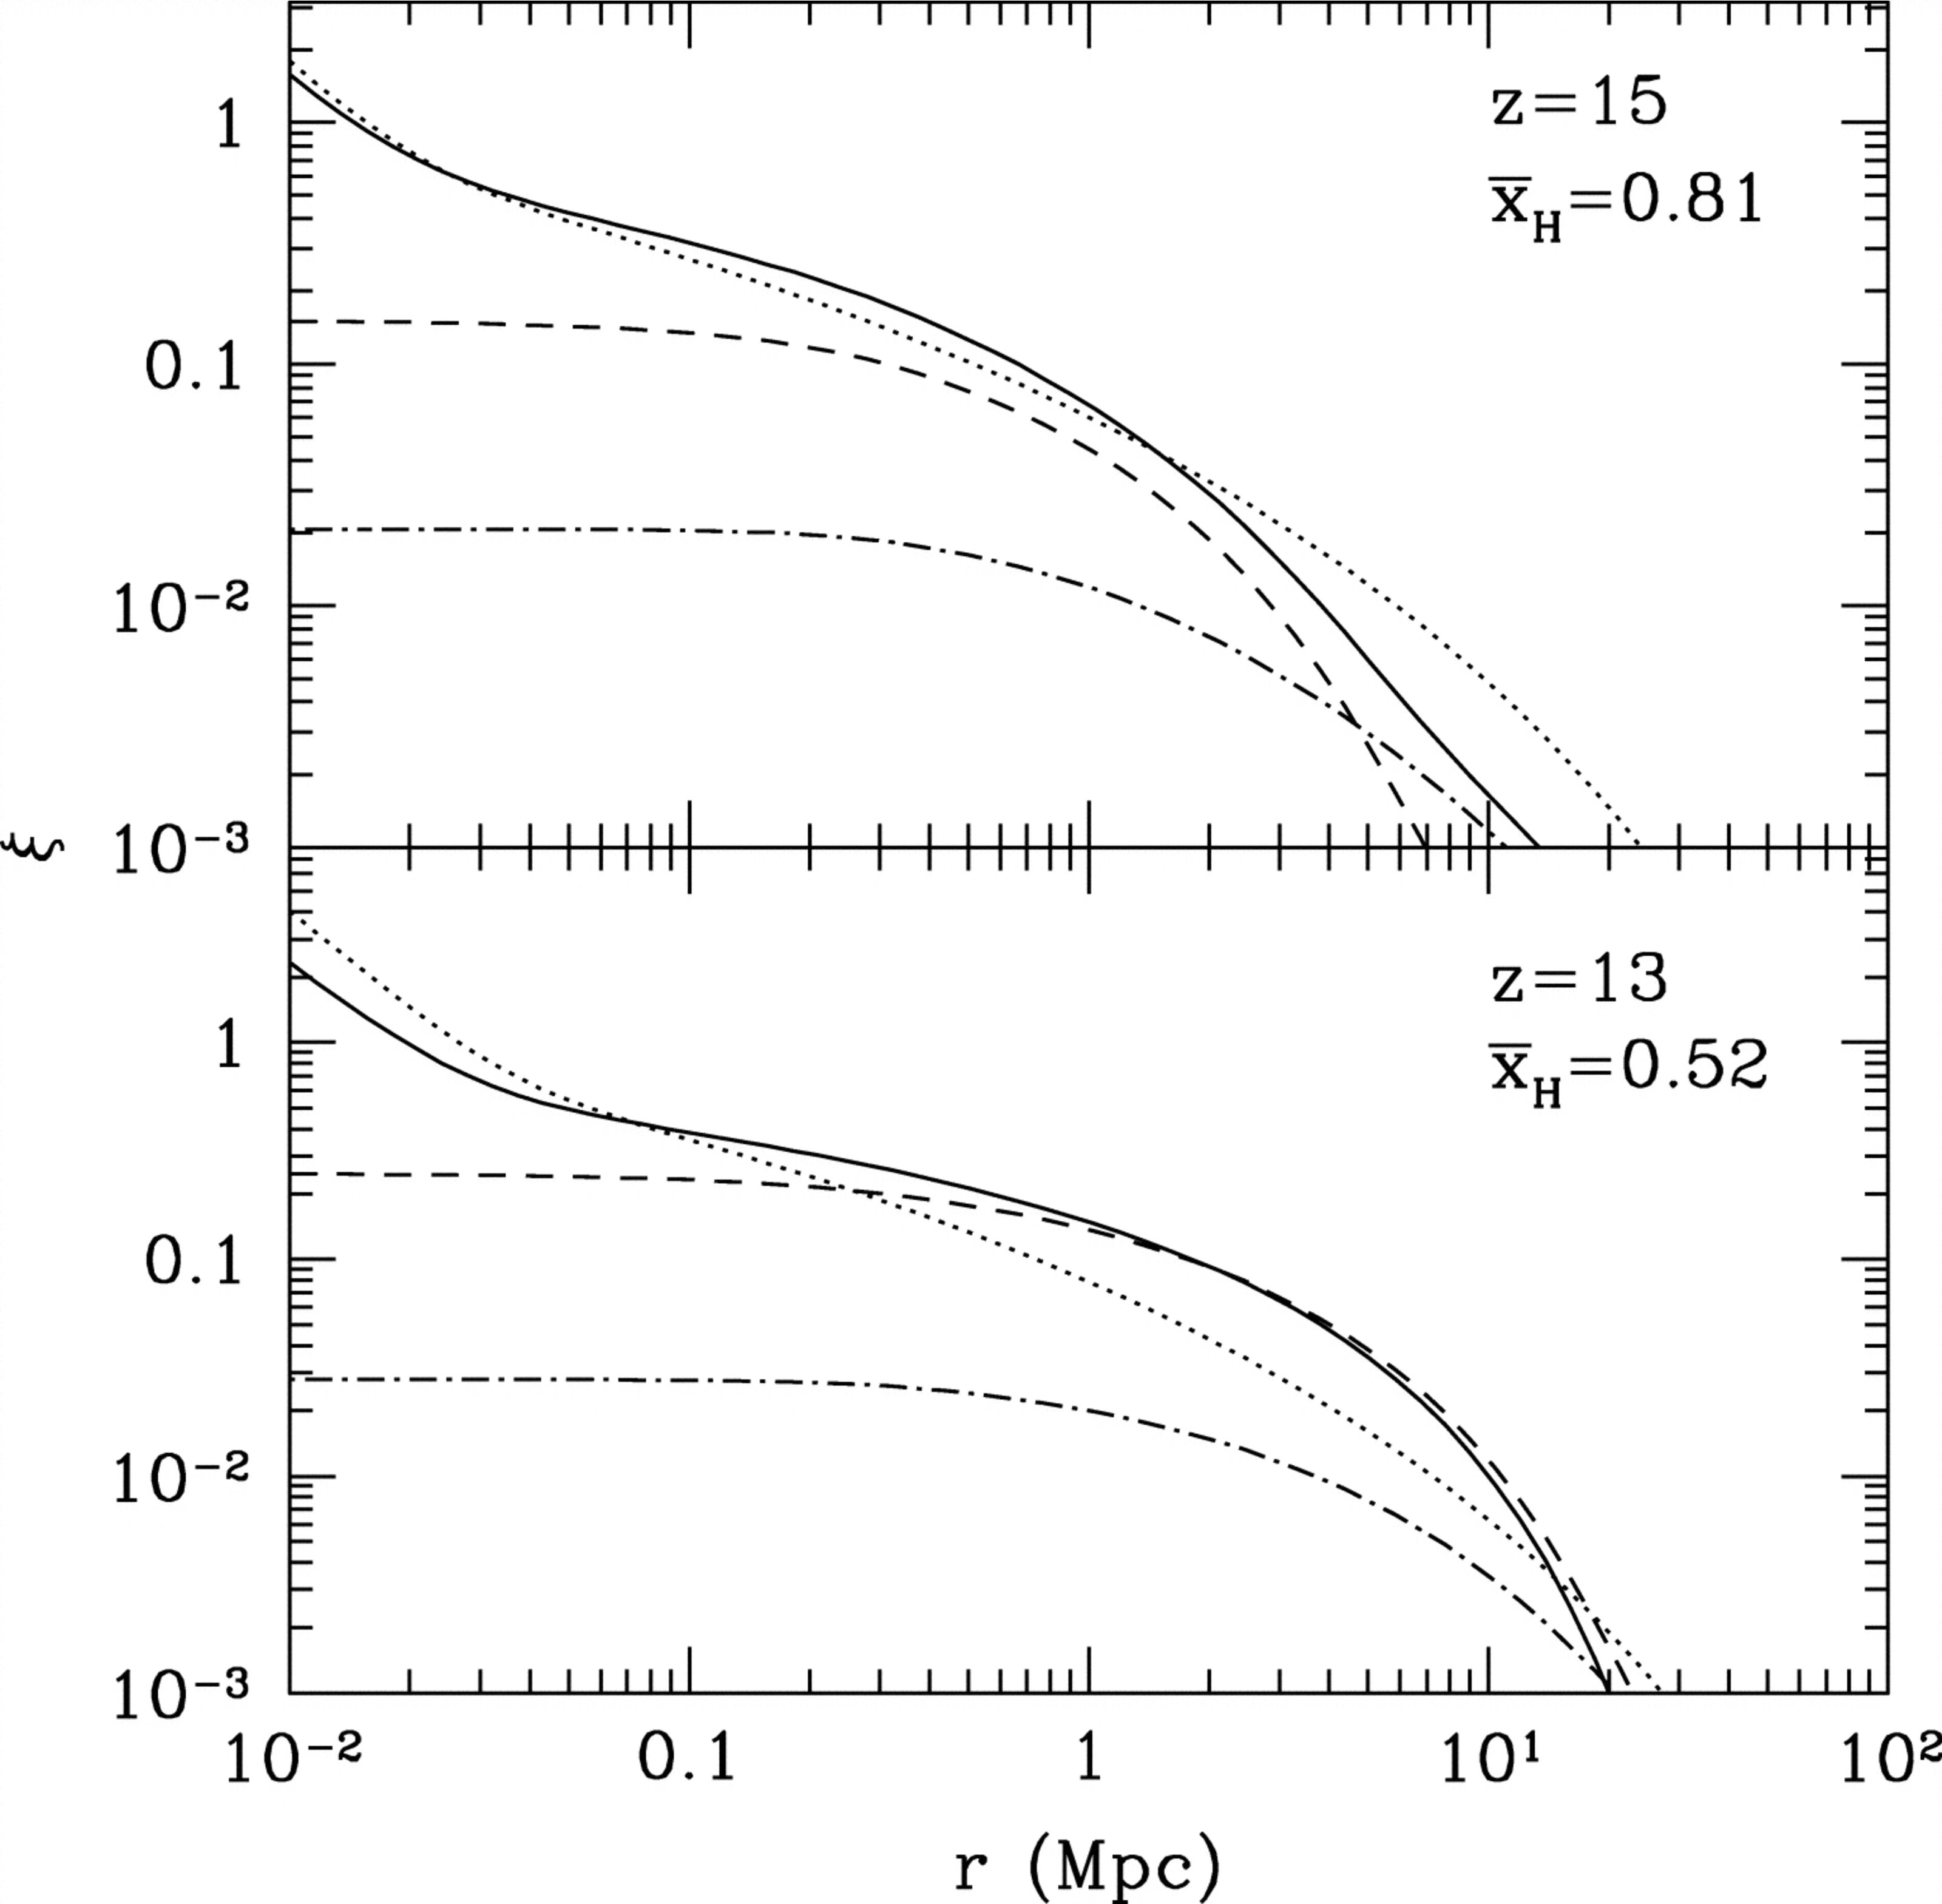
\includegraphics[width=0.3\textwidth]{Mirocha/fzh04_fig5.pdf} 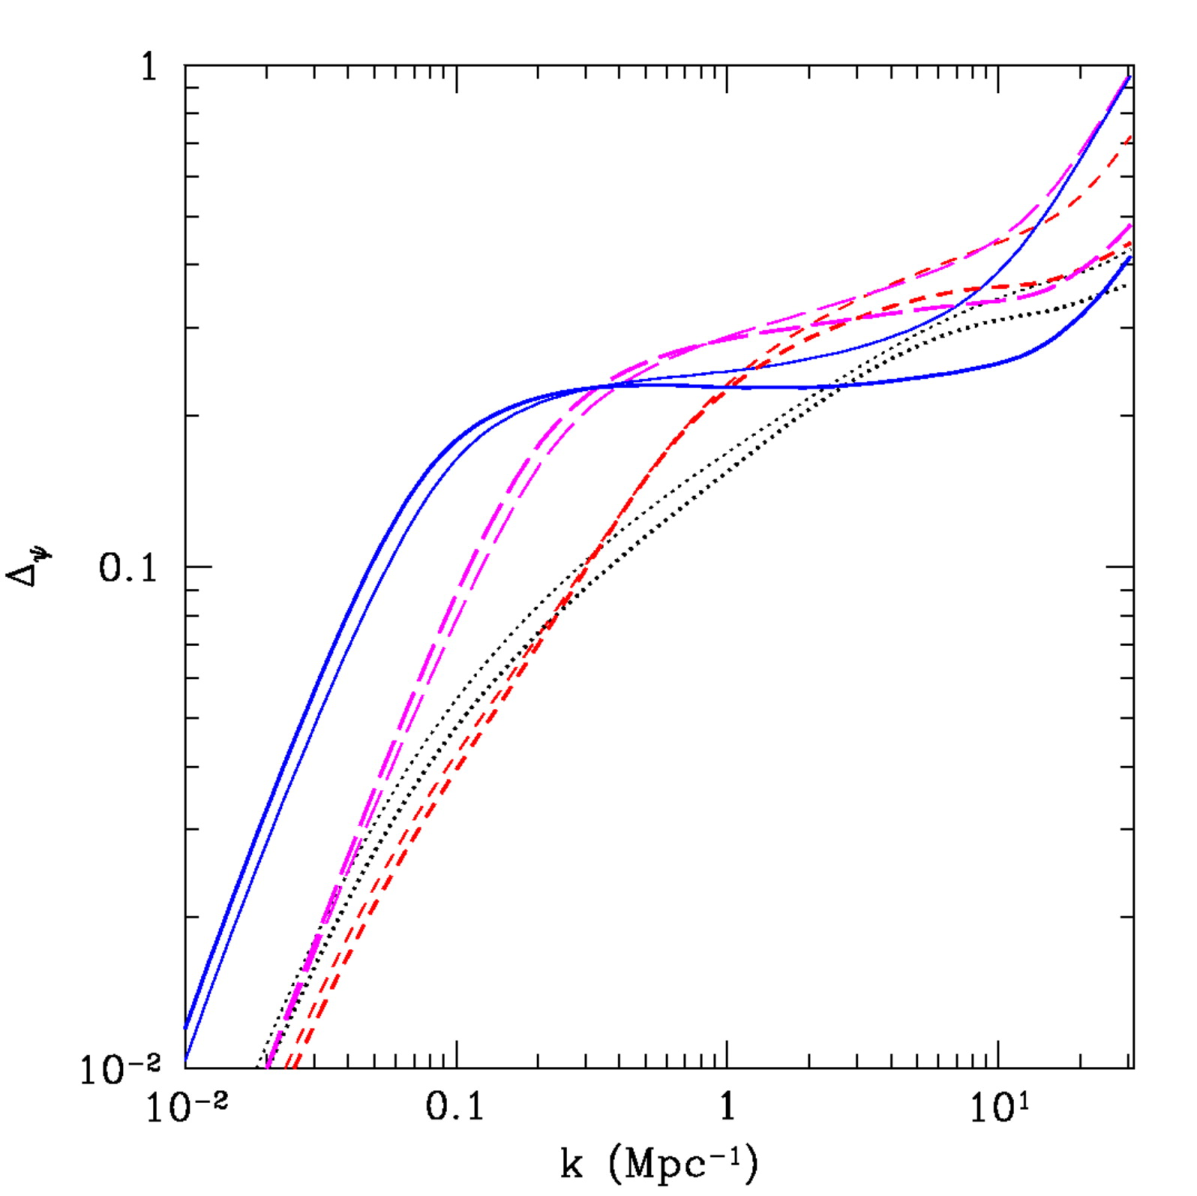
\includegraphics[width=0.3\textwidth]{Mirocha/fzh04_fig7.pdf}
\end{center}
\caption{{\bf Analytic models of bubble growth during the EoR \cite{Furlanetto2004}.} \textit{Left:} Bubble size distributions at bubble filling fractions of $Q=0.037, 0.11, 0.3, 0.5$, and 0.74, from left to right. \textit{Middle:} Correlation function of $\psi = \xHI (1 + \delta)$ (solid) at $\xHI=0.81$ (top) and $\xHI = 0.52$ (bottom) as well as its constituent components, including the ionization auto-correlation function (dashed), density auto-correlation function (dotted), and cross-correlation function between ionization and density (dot-dashed). \textit{Right:} Dimensionless power spectrum of $\psi$ for different values of $\zeta$, including $\zeta=12$ (thin) and $\zeta=40$ (thick), at several neutral fractions, $\xHI=0.96$ (dotted), 0.8 (short-dashed), 0.5 (long-dashed), and 0.26 (solid).}
\label{fig:fzh04}
\end{figure}

{\color{red} Things to mention here:
\begin{itemize}
	\item Photon conservation can be a problem.
	\item Dealing with overlap is a problem.
\end{itemize}}


%%
% RECOMBINATIONS
%%
\subsubsection{Recombinations}
{\color{red} Will need to describe the challenge here in some detail, defer to \S\ref{sec:predictions} for how one deals with this in semi-numeric and numerical simulations.}

%%
% 
%\subsubsection{Effects of Helium Reionization}
%HeI and HI likely re-ionize at the same time....HeII later.

%Mention correction factor $A_{\mathrm{He}}$ that one often sees in papers?

%%
% EVOLUTION EQUATIONS. II. Temperature
%%
\subsection{The (Kinetic) Temperature Field}

% Mean temperature
\subsubsection{Global Evolution} \label{sec:temperature_global}
The largely binary nature of the ionization field results in models designed to describe the fractional volume of ionized gas and the size distribution of individual ionized regions. This binarity will be reflected in the temperature field as well given that ionized regions are $\sim 10^4$ K, while the rest of the IGM will generally be much cooler. However, given that the 21-cm background is insensitive to the temperature within ionized regions, in what follows the mean kinetic temperature will \textit{not} refer to a volume-averaged temperature, but rather the average temperature of gas outside fully-ionized regions. 

Modeling the temperature in the bulk of the IGM in general is best handled by radiative transfer simulations. However, such simulations can be even more challenging than those targeting the ionization field given that (i) the mean-free paths of relevant photons are longer, (ii) the frequency-dependence of the ionization and heating rates is important, which means multi-frequency calculations are necessary, and (iii) heating generally precedes reionization, meaning smaller halos must be resolved at earlier times. 

Due to the immense computational challenge in simulating X-ray heating, most models still employ approximate techniques. It is useful to consider first a case in which heating of the IGM is perfectly spatially uniform, which could be a good approximation if the sources of heating have very hard spectra. In this limit, the solutions to the radiative transfer equation outlined in \S\ref{sec:largescales} apply, i.e., the mean intensity of the background radiation field is used to determine the heating rate density of the bulk IGM. 

{\color{red} Show simple models a la Pritchard \& Loeb.}

Talk about tradeoff between hard x-rays and soft x-rays.


% Fluctuations in the temperature
\subsubsection{Spatial Structure} \label{sec:temperature_local}
While photons with energies $h\nu \gtrsim 2$ keV can travel cosmological distances (see Eq. \ref{eq:mfp}), softer X-rays will be absorbed on $\sim 0.1-10$ cMpc scales and drive fluctuations in the temperature field. As a result, temperature profiles around individual sources exhibit very extended structures -- in contrast to the sharp edges characteristic of HII regions -- which results in extended structures in the 21-cm brightness temperature as well. 

One dimensional radiative transfer simulations nicely illustrate the basic expectations for heating around X-ray sources. In Figure XYZ, we show radial profiles of the kinetic temperature and 21-cm brightness temperature for power-law sources of X-rays. Note that plateau in temperature on small scales, indicative of a fully-ionized medium, that gradually transitions to temperatures $\TK < \Tcmb$ over $\sim$ Mpc scales. The gradient in temperature beyond the edge of the ionized bubble depends on the hardness of the X-ray spectrum: harder spectra produce sharper gradients because the typical mean free paths of photons is long \cite{Thomas2008,Knevit2014,Mirocha2012,McQuinn2012}. Detailed 21-cm maps may thus constrain source spectra through measurements of the 21-cm brightness temperature gradient on the outskirts of ionized bubbles \cite{Kramer2008}. Such signatures may be discernible in the 21-cm power spectrum as well \cite{Pacucci2014}.

There are many different strategies for extending X-ray heating to fully cosmological calculations. The most accurate is of course to perform RT ``on the fly'' in cosmological hydrodynamical simulations \cite{Xu2014}, though such calculations have only been carried out in large $\sim 100$ Mpc boxes recently \cite{Ross2017}. Efficient methods are still very much necessary in order to more fully explore the parameter space, and to build intuition for the results of more expensive calculations.

The most straightforward approach conceptually is to build libraries of 1-D results, i.e., radial profiles of ionization and temperature around sources of varying brightness and spectral characteristics, and ``paint'' them onto halos from N-body simulations \cite{Thomas2009}. The main challenge for such methods is how to modify the profiles of sources when their ionization and heating profiles overlap. Such methods also cannot self-consistently handle density fluctuations, which are absent in the library-building stage. Despite these challenges, workarounds do exist and can result in qualitatively reasonable 21-cm predictions \cite{Thomas2009}. 

A similar approach in spirit is to approach the problem statistically, foregoing the possibility of generating 21-cm maps and focusing instead solely on the statistics of the 21-cm field. Taking inspiration from 1-D RT models, one can construct a ``mask'' that relates temperature fluctuations to the density field. {\color{red} Talk about Jonathan's 2007 approach, Janakee's stuff.}

{\color{red} Show example masks and power spectra.}

The solution adopted in several semi-numerical simulations in recent years is a compromise between RT simulations, 1-D / N-body hybrids, and analytic methods. Rather than adopting a ``source centric'' model, in which radiation is propagated outward from sources until fully attenuated, one iterates through volume elements and sums radiation in concentric spherical shells along the past lightcone. 

{\color{red} Show equation here?}

The main challenge here is how to compute the opacity between source shells and the point of interest. In \textsc{21cmfast} \cite{Mesinger2011}, the opacity is computed assuming the cosmic mean density and the volume-averaged ionization fraction. This approach of course breaks down close to ionized regions. To avoid this problem, \cite{Fialkov2015} instead use the ionized fraction averaged within the sphere of interest, resulting in opacities that are sensitive to the local ionization field, and should more accurately capture the temperature close to ionized regions. In either case, the interplay between X-rays and the density field cannot be captured as it requires ray tracing. As a result, detailed radiative transfer calculations are still required to properly account for feedback between X-rays and the gas density. 

{\color{red} Takeaway points: sensitive to normalization and spectrum of sources}

%%
% EVOLUTION EQUATIONS. III. Ly-a coupling
%%
\subsection{The Ly-$\alpha$ Background}
The $\Lya$ background is the root cause of Wouthuysen-Field coupling, which  ``activates'' the 21-cm background when stars first flood the IGM with UV photons, driving the HI spin temperature toward the gas kinetic temperature. As a result, the 21-cm background probes the timing of when the first stars form and constrains their typical host halo masses through $\TS$, mean $\Lya$ intensity, $J_{\alpha}$, and fluctuations.


% GLOBAL EVOLUTION
\subsubsection{Global Evolution} \label{sec:lya_global}
The mean $\Lya$ background intensity, $J_{\alpha}$, requires a special solution to the cosmological radiative transfer equation (see Eq. \ref{eq:rte_diffeq}). Two effects separate this problem from the generic transfer problem outlined in \S\ref{sec:largescales}: (i) the Lyman series forms a set of horizons for photons in the $10.2 < h \nu / \mathrm{eV} < 13.6$ interval, giving rise to the so-called ``sawtooth modulation'' of the soft UV background \cite{Haiman1997}, and (ii) the Ly-$\alpha$ background is sourced both by photons redshifting into the line resonance as well as those produced in cascades downward from higher $n$ transitions \cite{Pritchard2006}.

As a result, it is customary to solve the RTE in each $\Lyn$ frequency interval separately. Within each interval, bounded by Ly-$n$ line on its red edge and Ly-$n+1$ on its blue edge, the optical depth is small in a primordial medium because no photon redward of the Lyman edge can ionize hydrogen or helium\footnote{There is in principle a small opacity contribution from $H_2$, though we neglect this in what follows as the $H_2$ fraction in the IGM is expected to be small.}. As a result, any photon starting its journey just redward of Ly-$\beta$ will travel freely until it redshifts into the Ly-$\alpha$ resonance, while photons originating at bluer wavelengths will encounter Ly-$n$ resonances (with $n>2$), only a fraction of which will ultimately result in $\Lya$ photons.

We can thus write the $\Lya$ background intensity as
\begin{equation}
    \widehat{J}_{\alpha}(z) = \frac{c}{4\pi} (1 + z)^2 \sum_{n = 2}^{\nmax} \frecn \int_z^{z_{\max}^{(n)}} \frac{\epsilon_{\nu}^{\prime}(z^{\prime})}{H(z^{\prime})} dz^{\prime} \label{eq:LymanAlphaFlux}
\end{equation}
where $\frecn$ is the ``recycling fraction,'' that is, the fraction of photons that redshift into a Ly-$n$ resonance that ultimately cascade through the $\Lya$ resonance \cite{Pritchard2006}. The upper bound of the definite integral,
\begin{equation}
    1 + z_{\max}^{(n)} = (1 + z) \frac{\left[1 - (n + 1)^{-2}\right]}{1 - n^{-2}} ,
\end{equation}
is set by the horizon of $\Lyn$ photons -- a photon redshifting through the  $\Lyn$ resonance at $z$ could only have been emitted at $z^{\prime} < z_{\max}^{(n)}$, since emission at slightly higher redshift would mean the photon redshifted through the $\text{Ly}(n+1)$ resonance. The sum over Ly-$n$ levels in Eq. \ref{eq:LymanAlphaFlux} is generally truncated at $n_{\max}=23$ \cite{Barkana2005} since the horizon for such photons is smaller than the typical ionized bubble sourced by an individual galaxy. As a result, any $\Lya$ photons generated by such high-$n$ cascades are ``wasted'' as far as the spin temperature is concerned, as they will most likely have redshifted out of resonance before reaching any neutral gas. $\Lya$ emission produced by recombinations in galactic HII regions is generally neglected for the same reason. Though there are some assumptions built into the $n_{\max}$ estimate, the total $\Lya$ photon budget is relatively insensitive to the exact value of $n_{\max}$.

Note that in general the mean free path of photons between Lyman series resonances is very long, which makes tracking them in numerical simulations  extremely expensive, at least for ray tracing schemes. For example, a photon emitted just redward of Ly-$\beta$, and observed at the Ly-$\alpha$ frequency at redshift $z$ has traveled a distance
\begin{equation}
	d_{\beta\rightarrow \alpha} \simeq 200 \ h_{70}^{-1} \left(\frac{\Omega_{m,0}}{0.3} \frac{1+z}{20} \right)^{-1/2} \ \mathrm{cMpc},
\end{equation}
where we have assumed the high-$z$ approximation $\Omega_{\Lambda} \ll \Omega_m$. This exceeds a Hubble length at high-$z$, meaning most of the Wouthuysen-Field coupling at very early times must come from photons originating just blueward of their nearest $\Lyn$ resonance.

%%
% LyA fluctuations
%%
\subsubsection{Spatial Fluctuations in the Ly-$\alpha$ background}
Despite the long mean free paths of photons in the $10.2 \lesssim \nu/\mathrm{eV} \lesssim 13.6$ band, the $\Lya$ background still exhibits strong fluctuations due to the clustering of sources. Unlike the kinetic temperature field, which is sensitive to fluctuations in the opacity along sightlines to different sources, the $\Lya$ intensity is effectively an optically thin radiation field modified by the $\Lyn$ horizons (see previous discussion; \S\ref{sec:lya_global}). As a result, summing the emissions from sources in concentric spherical shells around the point of interest (including $r^{-2}$ dimming and sawtooth modulation) along the lightcone is an accurate way to determine the local $\Lya$ intensity. Indeed, this approach is taken in several 21-cm codes \cite{Mesinger2011,Fialkov2014b}. 

The basic structure in the $\Lya$ field is well-described by analytic models thanks to the effectively negligible IGM opacity and the fact that the radiative coupling coefficients depend only on the instantaneous $\Lya$ flux, in contrast to, e.g., the IGM temperature, which depends on the entire history of emission incident on some volume element. As a result, one can construct a model for $\Lya$ fluctuations from (i) a model for the density field and how it is populated by sources and (ii) a model for the flux profile around individual sources, i.e., an inverse square law with Lyman series modulation.

Figure \ref{fig:holzbauer2012} shows a normalized profile for $J_{\alpha}$

\begin{figure*}[]
\begin{center}
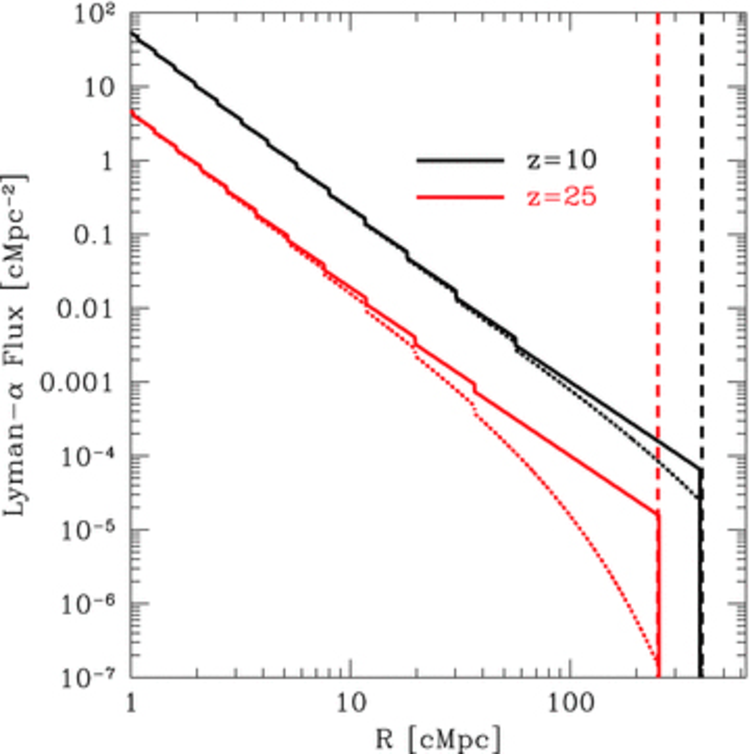
\includegraphics[width=0.49\textwidth]{Mirocha/holzbauer2012_fig7.pdf} 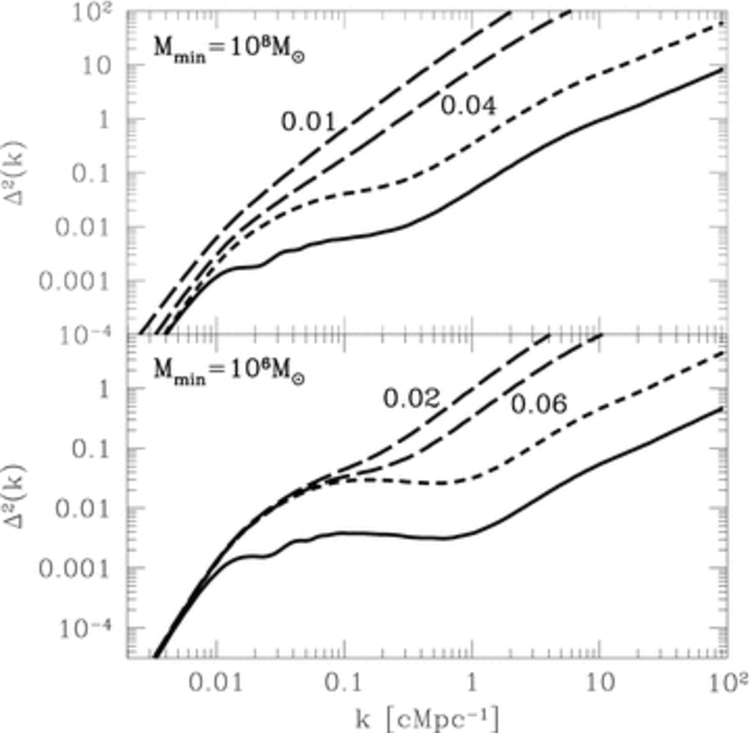
\includegraphics[width=0.49\textwidth]{Mirocha/holzbauer2012_fig9.pdf}
\end{center}
\caption{{\bf Fluctuations in the $\Lya$ background \cite{Holzbauer2012}.} \textit{Left:} Normalized $\Lya$ flux profile around a $10^8 \ M_{\odot}$ halo at $z=10$ and $z=25$. Dotted lines indicate solutions when light-cone effect is included. \textit{Right:} Dimensionless power spectrum of the $\Lya$ background for models in which the mean background $J_{\mathrm{LW}} = 0.1 J_{21}$ at $z=20.5$ (top) and $z=30.15$ (bottom). Short-dashed lines indicate inclusion of light-cone effects, while long-dashed lines indicate models with different duty cycles (indicated in plot).}
\label{fig:holzbauer2012}
\end{figure*}

{\color{red} Takeaway points: relatively insensitive to spectral shape, still sensitive to Nlw and source clustering.}

%%%
%% SOURCES
%%%
\section{Sources of the UV and X-ray Background} \label{sec:sources}
In the previous sections we outlined a procedure for evolving the ionization and temperature fields without actually specificying the sources of ionization and heating. Instead, we used a generic emissivity, $\epsilon_{\nu}$, to encode the integrated emissions of sources at frequency $\nu$ within some region $R$, which we will now write as an integral over the differential luminosity function of sources, i.e.,
\begin{equation}
	\epsilon_{\nu}(z,R) = \int_0^{\infty} dL_{\nu} \frac{dn}{dL_{\nu}} .
\end{equation}
It is common to rewrite the emissivity as an integral over the DM halo mass function (HMF), $dn/dm$, multiplied by a conversion factor between halo mass and galaxy light, $dm/dL_{\nu}$, i.e.,
\begin{equation}
	\epsilon_{\nu}(z,R) = \int_{\mmin}^{\infty} dm \frac{dn}{dm} \frac{dm}{d L_{\nu}} ,
\end{equation}
where $\mmin$ is the minimum mass of DM halos capable of hosting galaxies. Because $dn/dm$ is reasonably well-determined from large N-body simulations of structure formation \cite{PS1974,SMT2001,Tinker2010}, much of the modeling focus is on the mass-to-light ratio, $dm/dL_{\nu}$, which encodes the efficiency with which galaxies form in halos and the relative luminosities of different kinds of sources within galaxies (e.g., stars, compact objects, diffuse gas) that emit at different frequencies\footnote{Most models consider regions $R$ that are sufficiently large that one can assume a well-populated HMF, though at very early times this approximation may break down, rendering stochasticity due to poor HMF sampling an important effect.}. 

The main strength of the 21-cm background as a probe of high-$z$ galaxies is now apparent: though 21-cm measurements cannot constrain the properties of individual galaxies, they can constrain the properties of \textit{all} galaxies, in aggregate, \textit{even those too faint to be detected directly}. As a result, it is common to forego detailed modeling of the mass-to-light ratio and instead relate the emissivity to the fraction of mass in the Universe in collapsed objects,
\begin{equation}
	\epsilon_{\nu}(z, R) = \rho_b \fcoll(z, R) \zeta_{\nu} ,
\end{equation}
where the collapsed fraction is an integral over the HMF,
\begin{equation}
	\fcoll = \rho_m^{-1} \int_{\mmin}^{\infty} dm m \frac{dn}{dm}
\end{equation}
and $\zeta_{\nu}$ is an efficiency factor that quantifies the number of photons emitted at frequency $\nu$ per baryon of collapsed mass in the Universe. It is generally modeled as
\begin{equation}
	\zeta_{\nu} = f_{\ast} N_{\nu} f_{\esc,\nu} , \label{eq:zeta}
\end{equation}
where $f_{\ast}$ is the star formation efficiency (SFE), $N_{\nu}$ is the number of photons emitted per stellar baryon at some frequency $\nu$, and $f_{\esc}$ is the fraction of those photons that escape into the IGM. One could define additional $\zeta$ factors to represent, e.g., emission from black holes or exotic particles, in which case $f_{\ast}$ and $N_{\nu}$ would be replaced by some black hole or exotic particle production efficiencies. In practice, three $\zeta$ factors are defined: $\zeta$, $\zeta_X$, and $\zeta_{\alpha}$, i.e., one efficiency factor for each radiation background of interest. A minimal model for the 21-cm background thus contains four parameters: $\mmin$, $\zeta$, $\zeta_X$, and $\zeta_{\alpha}$. 

Because the factors within $\zeta$ are degenerate with each other, at least as far as 21-cm measurements are concerned, they generally are not treated separately as free parameters. However, it is still useful to consider each individually in order to determine a fiducial value of $\zeta$ and explore deviations from that fiducial model. In addition, inclusion of ancillary measurements may eventually allow $\zeta$ to be decomposed into its constituent parts \cite{Mirocha2017,Park2019,Greig2019}. For the remainder of this section, we focus on plausible values of $f_{\ast}$, $N_{\nu}$ and $f_{\esc}$.

%%
% PopII Star Formation
%%
\subsection{Star Formation} \label{sec:sfe}
Current high-$z$ measurements support a relatively simple picture of star formation in early galaxies. The basic idea is that star formation is fueled by the inflow of gas from the IGM, but the overall rate of star formation in galaxies is self-limiting because winds and supernovae explosions expell gas that would otherwise form stars ({\color{red} many many references}). Qualitatively, the need for some kind of feedback is apparent simply from the mismatch in shapes between the halo mass function and galaxy luminosity function, the latter of which is steeper at both the very bright and very faint ends. 

A common approach in recent years is to use a ``semi-empirical'' model, in which the mapping between galaxy light and host DM halo mass is parameterized flexibly, then constrained by fitting the model to empirical constraints on the galaxy population, e.g., galaxy luminosity functions (LFs) and stellar mass functions (SMFs) {\color{red} many many citations}. The basic building blocks of such models are drawn from N-body simulations, which provide estimates for halo abundances as a function of mass and time, i.e., the halo mass function (HMF), as well as the growth rates of individual halos \cite{McBride2009}. The simplest approach is to assume a 1:1 correspondence between DM halos and galaxies, and then ``abundance match'' halos with galaxies, i.e.,
\begin{align}
	n(>L_h) & = \int_L^{\infty} \frac{dn}{dL^{\prime}} dL^{\prime} \nonumber \\
	& = n(>M_h)  \nonumber \\
	& = \int_{M_h}^{\infty} \frac{dn}{dM_h^{\prime}} dM_h^{\prime} .
\end{align}
This procedure reveals the mapping between mass and light, $dL/dM$, upon repeated integration over a grid of $L_h$ values, solving for the $M_h$ value needed for abundances to match.

In its simplest incarnation, abundance matching neglects the assembly histories of halos in detail. As a result, it is becoming more common to build forward models for galaxy formation that link galaxy star formation rate (SFR) to halo mass accretion rate, i.e.,
\begin{equation}
	\dot{M}_{\ast}(z,M_h) = f_{\ast}(z,M_h) \dot{M}_h (z,M_h) . \label{eq:SFE}
\end{equation}
The star formation efficiency, $f_{\ast}$, is left as a flexible function to be calibrated empirically, while the halo MAR, $\dot{M}_h$, is either drawn from the results of numerical simulations \cite{McBride2009,Trac2015}, or modeled approximately from the HMF itself \cite{Furlanetto2017}. 

To complete the link between halos and galaxies, one must adopt a conversion factor between SFR and galaxy luminosity in some band. High-$z$ measurements mostly probe the rest UV spectrum of galaxies, so it is customary to link the SFR with the rest $1600 \ \AA$ luminosity of galaxies,
\begin{equation}
	L_{1600}(z, M_h) = l_{1600} \dot{M}_{\ast}(z,M_h)
\end{equation}
where $l_{1600}$ is of order $10^{28} \ \mathrm{erg} \ \mathrm{s}^{-1} \ \mathrm{Hz}^{-1} \ (M_{\odot} / \mathrm{yr})^{-1}$ according to commonly-used stellar population synthesis models, assuming constant star formation \cite{Leitherer1999,Eldridge2009,Conroy2009}. The precise value depends on stellar metallicity, binarity, and initial mass function (IMF), and varies from model to model. We will revisit the details of stellar spectra in \S\ref{sec:UV}.

The end result of this exercise is a calibrated SFE curve, which can then be used to make predictions for galaxy properties too faint or too distant to have been detected by current surveys. A representative example \cite{Behroozi2019} is shown in Figure \ref{fig:universe_machine}. The rise and fall in the ratio of stellar mass to halo mass, $M_{\ast} / M_h$, is a generic result of semi-empirical models \cite{Trenti2010,Mason2015,Sun2016,Mashian2016,Tacchella2018}, indicating a change in how galaxies form stars in halos above and below $\sim 10^{12} \ M_{\odot}$. This trend is also consistent with the predictions of simple stellar feedback arguments, at least on the low-mass side of the SMHM peak \cite{Dayal2014,Furlanetto2017}.

\begin{figure*}[]
\begin{center}
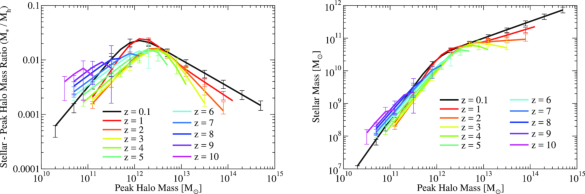
\includegraphics[width=0.98\textwidth]{Mirocha/behroozi2019_fig9.pdf}
\end{center}
\caption{{\bf Relationship between halos and star formation recovered by the \textsc{universemachine} \cite{Behroozi2019}.} \textit{Left:} Stellar mass (peak) halo mass relation. \textit{Right:} Stellar mass vs. (peak) halo mass.}
\label{fig:universe_machine}
\end{figure*}

While many studies now seek to simulate galaxy formation and reionization self-consistently using \textit{ab initio} cosmological simulations \cite{OShea2015,Gnedin2014}, such calculations are ill-suited to thorough parameter space explorations and inference. As a result, the semi-empirical approach to galaxy formation modeling is now becoming common in 21-cm modeling codes \cite{Mirocha2017,Park2019,Mutch2016}, as they lack the spatial resolution to model individual galaxies or even groups of galaxies. However, including some information about the galaxy population permits joint modeling of 21-cm observables as well as high-$z$ galaxy luminosity functions, stellar mass functions, and so on, and thus open up the possibility of tightening constraints on the properties of galaxies using a multi-wavelength approach.

%%
% PopIII
%%
\subsubsection{Pop~III Star Formation}
The very first generations of stars to form in the Universe did so under very different conditions than stars today, so it is not clear that the star formation model predictions/extrapolations outlined in the previous section apply. The first stars, by definition, formed from chemically-pristine material, since no previous generations of stars had existed to enrich the medium with heavy elements. This has long been recognized as a reason that the first stars are likely different than stars today \cite{Abel2000,Bromm1999}. Without the energetically low-lying electronic transitions common in heavy elements, hydrogen-only gas clouds cannot cool efficiently, as collisions energetic enough to excite atoms from $n=1$ to $n=2$ (which subsequently cool via spontaneous emission of $\Lya$ photons) imply temperatures of $\sim 10^4$ K. Setting $T_{\min} \sim 10^4$ K is thus a way to roughly exclude the effects of PopIII-hosting ``minihalos'' in a 21-cm model. 

Even in the absence of metals, there are cooling channels available even in halos too small to support atomic (hydrogen) line cooling. Hydrogen molecules, $\Htwo$, can form using free electrons as a catalyst\footnote{Dust is the primary catalyst of $\Htwo$ formation in the local Universe, but of course is does not exist in the first collapsing clouds.}, 
\begin{align}
	\Hatom + e^- & \rightarrow \Hatom^- + h\nu \\
	\Hatom^- + \Hatom & \rightarrow \Htwo + e^- ,
\end{align}
These reactions are limited by the availability of free electrons\footnote{
Exotic models in which an X-ray background emerges before the formation of the first stars may affect early star formation by boosting the electron fraction.} and the survivability of $\Hminus$ ions. Even in the absence of astrophysical backgrounds, the formation of $\Htwo$ is limited by the CMB, which at the high redshifts of interest can dissociate the $\Hminus$ ion. \cite{Tegmark1997} found that the molecular hydrogen fraction in high-$z$ halos scales with the virial temperature as
\begin{equation}
	f_{\Htwo} \approx 3.5 \times 10^{-4} \left(\frac{\Tvir}{10^3 \ \mathrm{K}} \right)^{1.52} .
\end{equation}
Once the first stars form, the situation grows considerably more complicated. As will be detailed in the following section (\S\ref{sec:UV}), massive stars are prodigious sources of UV photons. Some of these photons originate in the Lyman-Werner band ($\sim 11.2$-$13.6$ eV), and are thus capable of dissociating molecular hydrogen. This processs is expected to quickly surpass $\Hminus$ dissociation by the CMB as the most important mechanism capable of regulating star formation in chemically pristine halos\footnote{If the PopIII IMF is very bottom-heavy, the resulting IR background  could continue to regulate star formation via $\Hminus$ photo-detachment \cite{WolcottGreen2012}.}. 

A substantial literature has emerged in the last $\sim 20$ years aimed at understanding the critical LW background intensity, $\JLW$, required to prevent star formation in high-$z$ minihaloes. For example, \cite{Visbal2014} find
\begin{equation}
	M_{\mathrm{crit}} = 2.5 \times 10^5 \left(\frac{1+z}{26} \right)^{-3/2} (1 + 6.96(4\pi \JLW)^{0.47})  \ \Msun
\end{equation}
where $\JLW$ is the LW background intensity in units of $10^{-21} \ \mathrm{erg} \ \mathrm{s}^{-1} \ \mathrm{cm}^{-2} \ \mathrm{Hz}^{-1} \ \mathrm{sr}^{-1}$. In principle, $M_{\mathrm{crit}}$ varies across the Universe from region to region as a function of the local LW intensity, but it is common to use the mean LW background intensity for simplicity. Note finally that sufficiently dense clouds may be able to self-shield themselves against LW radiation, so $\JLW$ is subject to reduction by a factor of $f_{\mathrm{sh}}$ \cite{WolcottGreen2011}.

While the LW background is responsible for setting the \textit{minimum} halo mass required to host star formation, the \textit{maximum} mass of Pop~III halos, i.e., the mass at which halos transition from Pop~III to Pop~II star formation, depends on the interplay of many complex processes. For example, Pop~III supernovae will inject metals into the ISM of their host galaxies, which can trigger the transition to Pop~II star formation provided that at least some metals are retained and efficiently mix into proto-stellar clouds. The timescales involved are highly uncertain and may vary from halo to halo. As a result, whereas UVLFs at high-$z$ provide some insight into the Pop~II SFE, the Pop~III SFE, which encodes the complex feedback processes at play, is completely unknown. 

{\color{red} Show some models for the PopIII SFRD and compare to PopII SFRD extrapolated from observations and/or predictions from models.}


In 21-cm models it is common to neglect a detailed treatment of individual Pop~III star-forming halos, and instead parameterize the impact of Pop~II and Pop~III halos separately. One way to do this is to assume all atomic cooling halos form Pop~II stars (with $\zeta_{LW,\textsc{ii}}$, $\zeta_{X,\textsc{ii}}$, etc.), and all minihalos form Pop~III, with their own efficiency factors $\zeta_{X,\textsc{ii}}$ etc., and $\mmin$ determined self-consistently from the emergent LW background intensity \cite{Fialkov2014a,Mirocha2018}. We will revisit the predictions of these models in \S\ref{sec:predictions}. 


% STARS
\subsection{UV Emission from Stars} \label{sec:UV}
Stellar photons are likely the dominant drivers of reionization\footnote{Though see \cite{Madau2015} for discussion of a quasar-dominated scenario.} and the initial ``activation'' of the 21-cm background via Wouthuysen-Field coupling at $z \sim 30$. The 21-cm background is thus sensitive to the spectral characteristics of stars in the Lyman continuum and Lyman Werner bands\footnote{We use this definition here loosely. Technically, the LW band is $\sim 11.2-13.6$ eV, a range which bounds photons capable of photo-dissociating molecular hydrogen, $H_2$. The $\Lya$ background is sourced by photons in a slightly broader interval, $\sim 10.2-13.6$ eV, but it is tedious to continually indicate this distinction, and as a result, we use ``LW band'' to mean all photons capable of eventually generating $\Lya$ photons.}. It is also in principle sensitive to the spectrum of even harder He-ionizing photons, since photo-electrons generated from helium ionization can heat and ionize the gas, while HeII recombinations can result in H-ionizing photons. The 21-cm signal could in principle even constrain the rest-frame infrared spectrum of stars in the early Universe, since IR photons can feedback on star-formation at very early times through $\Hminus$ photo-detachment \cite{WolcottGreen2012}. In this section, we focus only on the soft UV spectrum ($E < 54.4$ eV) to which the 21-cm background is most sensitive.

The most detailed predictions for stellar spectra come from stellar population synthesis (SPS) models, which take the following approach:
\begin{itemize}
	\item Assume a model for the stellar initial mass function (IMF), $\xi(m)$, i.e., the number of relative number of stars formed in different mass bins. Commonly-adopted IMFs include Salpeter \cite{Salpeter1955}, Chabrier \cite{Chabrier2003}, Kroupa \cite{Kroupa2001}, and Scalo \cite{Scalo1998} which are all generally power-laws with indices $\sim -2.3$ , but differing in shape at the low mass end of the distribution ($M_{\ast} < 0.5 \ \Msun$ ).
	\item Assume a model for stellar evolution, i.e., how stars of different masses traverse the Hertzprung-Russell (HR) diagram over time.
	\item Assume a model for stellar atmospheres, i.e., as a function of stellar mass, age, and composition, determine the output spectrum.
\end{itemize}
With all these ingredients, one can synthesize a spectrum from a population of stars with a given age,
\begin{equation}
	L_{\nu}(t) = \int_0^t dt^{\prime} \int_{\mmin}^{\infty} dm \xi(m) l_{\nu} (m, t^{\prime}) \label{eq:Lcluster}
\end{equation}
where $l_{\nu}(m, t)$ is the specific luminosity of a star of mass $m$ and age $t$, and we have assumed that $\xi$ is normalized to the mass of the star cluster, $\int dm \xi(m) = M_{\ast}$. Equation \ref{eq:Lcluster} can be generalized to determine the spectrum of a galaxy with an arbitrary star formation history (SFH) composed of discrete bursts. {\color{red} mention poor IMF sampling? Widely used stellar synthesis codes include \textsc{starburst99} \cite{Leitherer1999}, \textsc{bpass} \cite{Eldridge2009}, FSPS, Bruzual \& Charlot...}

Generally, 21-cm models do not operate at level of SPS models because the 21-cm background is insensitive to the detailed spectra and SFHs of individual galaxies. Instead, because 21-cm measurements probe the relatively narrow intervals $10.2 < h\nu / \mathrm{eV} < 13.6$ via Wouthuysen-Field coupling and $h\nu > 13.6$ eV through the ionization field, it is common to distill the predictions of SPS models into just two numbers, $\Nion$ and $N_{\alpha}$, which integrate over age and the details of the stellar SED, i.e.,
\begin{align}
	\Nion & = m_{\ast}^{-1} \int_0^{\infty} dt^{\prime} \int_{\nuLL}^{\infty} \frac{d\nu}{h\nu} L_{\nu}(t^{\prime}) \\
	N_{\alpha} & = m_{\ast}^{-1} \int_0^{\infty} dt^{\prime} \int_{\nuLya}^{\nuLL} \frac{d\nu}{h\nu} L_{\nu}(t^{\prime})
\end{align}
where $\nuLL$ is the frequency of the Lyman limit (13.6 eV) and $\nuLya$ is the Ly-$\alpha$ frequency. UV emission is dominated by massive, short-lived stars, hence the integration from $t=0$ to $t=\infty$.

Assuming a Scalo IMF, stellar metallicity of $Z=Z_{\odot}/20$, using \textsc{starburst99} SPS model, \cite{Barkana2005} report $N_{\alpha}=9690$, further broken down into sub-intervals between each Ly-$n$ resonance, an oft-used reference value even today. The general expectation is for $\Nion$ and $N_{\alpha}$ increase for more top-heavy IMF and lower metallicity, meaning these values are likely to increase for Pop~III stars ({\color{red} citations}). Similarly, binary evolution can effectively increase the lifetimes of massive stars, leading to a net gain in UV photon production \cite{Stanway2016}.


%%
% fesc
%%
\subsection{Escape of UV Photons from Galaxies}
The ionization state of intergalactic gas is of course influenced only by the ionizing photons that are able to escape from galactic halos. The fraction of photons that escape relative to the total number produced is quantified by the escape fraction, $\fesc$, and is the final component of the ionizing efficiency, $\zeta$, introduced previously. 

Current constraints on high-$z$ galaxies and reionization suggest that $\fesc$ must be $\sim 10-20\%$ \cite{Robertson2015}. The result is model-dependent, however, as it relies on assumptions about the UV photon production efficiency in galaxies and extrapolations to source populations beyond current detection limits. For example, if $\fesc$ depends inversely on halo mass, reionization can be driven by galaxies that have yet to be detected directly \cite{Finkelstein2018}. This scenario is appealing because it can explain (i) the very gradual evolution in the post-reionization ionizing background, and (ii) the apparently low-level of ionizing photon escape in galaxies at $3 \lesssim z \lesssim 6$ \cite{Shapley2003}. 

More recent observational programs have found some evidence for substantial escape fractions, $\fesc \sim 50\%$, at least in a subset of objects ({\color{red} citations}). This may be an indicator that photons escape is driven by patchiness in the HI gas distribution within galaxies -- if we happen to observe galaxies along clear channels through the ISM, we infer high $\fesc$, but from a slightly different vantage point we infer $\fesc \approx 0$. 

Predictions for $\fesc$ are now largely in the realm of numerical simulations, many of which lend credence to the idea that low-mass halos may have higher escape fractions \cite{Kimm2014}. The basic trend is sensible: as the depth of halo potentials declines, supernovae explosions can more easily excavate clear channels through which photons escape. However, there is far from a consensus on this issue. For example, the \textsc{FIRE} simulations do not see evidence that $\fesc$ depends on halo mass \cite{Ma2015}. This result, coupled with the very high resolution in \textsc{FIRE}, is more suggestive of a scenario in which $\fesc$ is set by very small-scale structure in the ISM, which knows nothing of the gravitational potential of the host halo. 

21-cm measurements in principle open a new window into constraining $\fesc$. If, for example, the UV/SFR conversion factor is well known, joint fitting 21-cm power spectra and high-$z$ galaxy LFs can isolate $f_{\ast}$ and $\fesc$ \cite{Park2019,Greig2019}. Note, however, that this is still model-dependent, as $f_{\ast}$ and $\fesc$ must both be extrapolated to some limiting UV magnitude or halo mass. 


%%%
%% BHs ETC
%%%
\subsection{X-rays from Black Holes}
Though stars themselves emit few photons at energies above the HeII-ionizing edge ($\sim 54.4$ eV), their remnants can be strong X-ray sources. While solitary remnants will be unlikely to accrete much gas from the diffuse ISM, remants in binary systems may accrete gas from their companions, either via Roche-lobe overflow or stellar winds. Such systems are known as X-ray binaries (XRBs), further categorized by the mass of the donor star: ``low-mass X-ray binaries'' (LMXBs) are those fueled by Roche-lobe overflow from a low-mass companion, while ``high-mass X-ray binaries'' (HMXBs) are fed by the winds of massive companions. XRBs exhibit a rich phenomenology of time- and frequency-dependent behavior and are thus interesting in their own right. For a review see, e.g., \cite{Remillard2006}.

In nearby star-forming galaxies, the X-ray luminosity is generally dominated by the HMXBs \cite{Gilfanov2004,Fabbiano2006,Mineo2012a}. Furthermore, the total luminosity in HMXBs scales with the star formation rate, as expected given that the donor stars in these systems are massive, short-lived stars. An oft-used result in the 21-cm literature stems from the work of \cite{Mineo2012a}, who find
\begin{equation}
	L_X = 2.6 \times 10^{39} \left(\frac{\SFR}{M_{\odot} \ \mathrm{yr}^{-1}} \right) \ \mathrm{erg} \ \mathrm{s}^{-1} \label{eq:LxSFR_Mineo}
\end{equation}
where $L_X$ refers to the 0.5-8 keV band. This relation provides an initial guess for many 21-cm models, which add an extra factor $f_X$ to parameterize our ignorance of how this relation evolves with cosmic time. For example, \cite{Furlanetto2006} write
\begin{equation}
	L_X = 3 \times 10^{40} f_X \left(\frac{\SFR}{M_{\odot} \ \mathrm{yr}^{-1}} \right) \ \mathrm{erg} \ \mathrm{s}^{-1} , \label{eq:LxSFR_Furlanetto}
\end{equation}
which is simply Equation \ref{eq:LxSFR_Mineo} re-normalized to a broader energy range, $0.2 < h\nu/\mathrm{keV} < 3\times 10^4$, assuming a power-law spectrum with spectral index $\alpha_X=-1.5$, where $\alpha_X$ is defined by $L_E \propto E^{\alpha_X}$, with $L_E$ in energy units. 

The normalization of these empirical $L_X$-SFR relations are not entirely unexpected, at least at the order-of-magnitude level. For example, if one considers a galaxy forming stars at a constant rate, a fraction $f_{\bullet} \simeq 10^{-3}$ of stars will be massive enough ($M_{\ast} > 20 \ M_{\odot}$) to form a black hole assuming a Chabrier IMF. Of those, a fraction $\fbin$ will have binary companions, with a fraction $\fsurv$ surviving the explosion of the first star for a time $\tau$. If accretion onto these black holes occurs in an optically thin, geometrically-thin disk with radiative efficiency $\epsilon_{\bullet} = 0.1$ which obeys the Eddington limit, then a multi-color disk spectrum is appropriate and a fraction $f_{0.5-8}=0.84$ of the bolometric luminosity will originate in the 0.5-8 keV band. Finally, assuming these BHs are ``active'' for a fraction $\fact$ of the time, we can write \cite{Mirabel2011,Mirocha2018}
\begin{equation}
	L_X \sim 2 \times 10^{39} \mathrm{erg} \ \mathrm{s}^{-1} \left(\frac{\SFR}{\SFRunits} \right) \left(\frac{\epsilon_{\bullet}}{0.1}\right) \left(\frac{f_{\bullet}}{10^{-3}} \right) \left(\frac{\fbin}{0.5} \right) \left(\frac{\fsurv}{0.2} \right) \left(\frac{\tau}{20 \ \mathrm{Myr}} \right) \left(\frac{\fact}{0.1} \right) \left(\frac{f_{0.5-8}}{0.84} \right) . \label{eq:LxSFR}
\end{equation}
While several of these factors are uncertain, particularly $\fsurv$ and $\fact$, this expression provides useful guidance in setting expectations for high redshift. For example, it has long been predicted that the first generations of stars were more massive on average than stars today owing to inefficient cooling in their birth clouds. This would boost $f_{\bullet}$, and thus $L_X/\SFR$, so long as most stars are not in the pair-instability supernova (PISN) mass range, in which no remnants are expected. 

There are of course additional arguments not present in Eq. \ref{eq:LxSFR}. For example, the MCD spectrum is only a good representation of HMXB spectra in the ``high soft'' state. At other times, in the so-called ``low hard'' state, HMXB spectra are well fit by a power-law. The relative amount of time spent in each of these states is unknown. Figure \ref{fig:xray_seds} compares typical HMXB spectra with the spectrum expected from hot ISM gas (see \S\ref{sec:ism_bremms}).

In addition, physical models for the $L_X$-SFR relation may invoke the metallicity as a driver of changes in the relation with time and/or galaxy (stellar) mass. As the metallicity declines, one might expect the stellar IMF to change (as outlined above), however, the winds of massive stars responsible for transferring material to BHs will also grow weaker as the opacity of their atmospheres decline. As a result, increases in $L_X$/SFR likely saturate below some critical metallicity. Observations of nearby, metal-poor dwarf galaxies support this picture, with $L_X$/SFR reaching a maximum of $\sim 10$ times the canonical relation quoted in Eq. \ref{eq:LxSFR_Mineo} \cite{Mineo2012a}.

%{\color{red} Left to discuss:
%\begin{itemize}
%	\item Observational limits on $L_X$/SFR from Chandra stacks?
%	\item Low metallicity constraints.
%\end{itemize}}

%%
% PopIII
%%
\subsubsection{Super-Massive Black Holes}
Though super-massive black holes (SMBHs) are exceedingly rare and thus unlikely to contribute substantially to the ionizing photon budget for reionization, fainter -- but more numerous -- intermediate mass black holes (IMBHs) with $10^3 \lesssim M_{\bullet} / M_{\odot} \lesssim 10^6$ could have a measureable impact on the IGM thermal history \cite{Tanaka2016}. Growing black holes, if similar to their low-$z$ counterparts, could also generate a strong enough radio background to amplify 21-cm signals \cite{EwallWice2018}, possibly providing an explanation for the anamalous depth of the EDGES global 21-cm measurement \cite{Bowman2018}. Such scenarios cannot yet be ruled out via independent measurements. For example, the unresolved fraction of the cosmic X-ray background still permits a substantial amount of accretion at $z \gtrsim 6$ \cite{McQuinn2012,Fialkov2017,Mirocha2018}, while just $\sim 10$\% of the radio excess reported by ARCADE-2 \cite{Fixsen2011,Singal2018} must originate at $z \gtrsim 18$ in order to explain the EDGES signal \cite{Feng2018}. Given the persistent challenge in explaining the existence of SMBHs at $z \gtrsim 6$, the signatures of BH growth in the 21-cm background are worth exploring in more detail.



% Hot gas
\subsection{X-rays from Shocks and Hot Gas} \label{sec:ism_bremms}
While compact remnants of massive stars are likely the leading producer of X-rays in high-$z$ star-forming galaxies, the supernovae events in which these objects are formed may not be far behind. Supernovae inject a tremendous amount of energy into the surrounding medium, which then cools either via inverse Compton emission (in supernova remnants; \cite{Oh2001}) or eventually via bremsstrahling radiation (in the hot interstellar medium; ISM. Because these sources are related to the deaths of massive stars their luminosity is expected to scale with SFR, as in the case of HMXBs. Indeed, \cite{Mineo2012b} find that diffuse X-ray emission in nearby sources follows the following relation in the 0.5-2 keV band:
\begin{equation}
	L_X = 8.3 \times 10^{38} \left(\frac{\SFR}{M_{\odot} \ \mathrm{yr}^{-1}} \right) \ \mathrm{erg} \ \mathrm{s}^{-1} \label{eq:LxSFRII_Mineo}
\end{equation}
This luminosity is that from all unresolved emission, and as a result, is not expected to trace emission from the hot ISM alone. Emission from supernova remnants will also contribute to this luminosity, as will fainter, unresolved HMXBs and LMXBs. \cite{Mineo2012b} estimate that $\sim 30-40$\% of this emission may be due to unresolved point sources. 


\begin{figure*}[]
\begin{center}
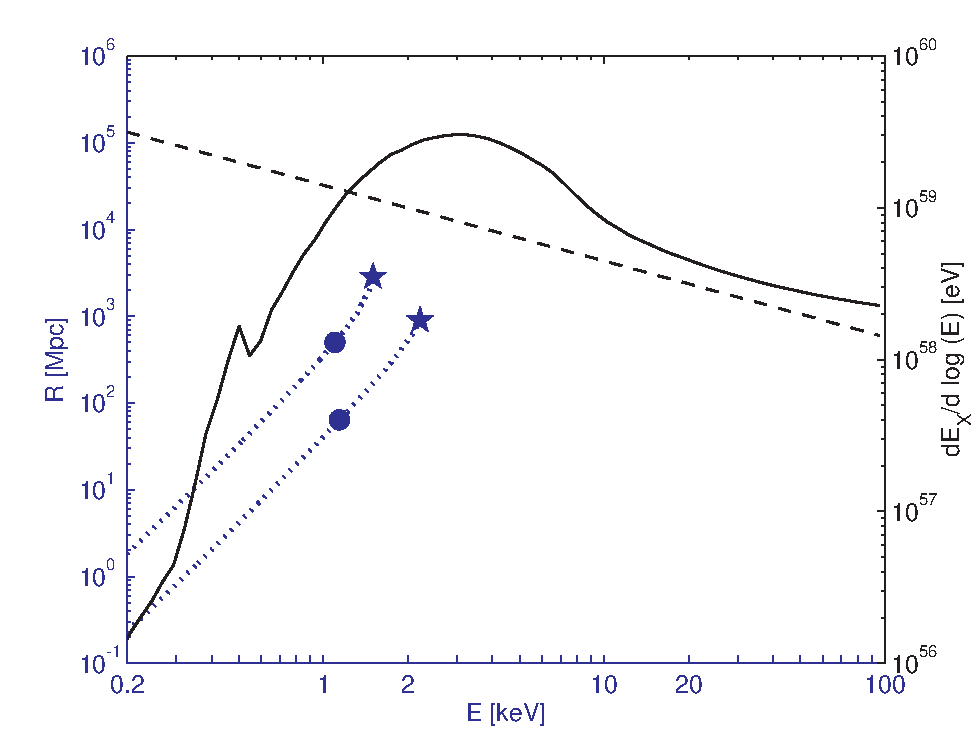
\includegraphics[width=0.49\textwidth]{Mirocha/fialkov2014_cygx1.pdf}
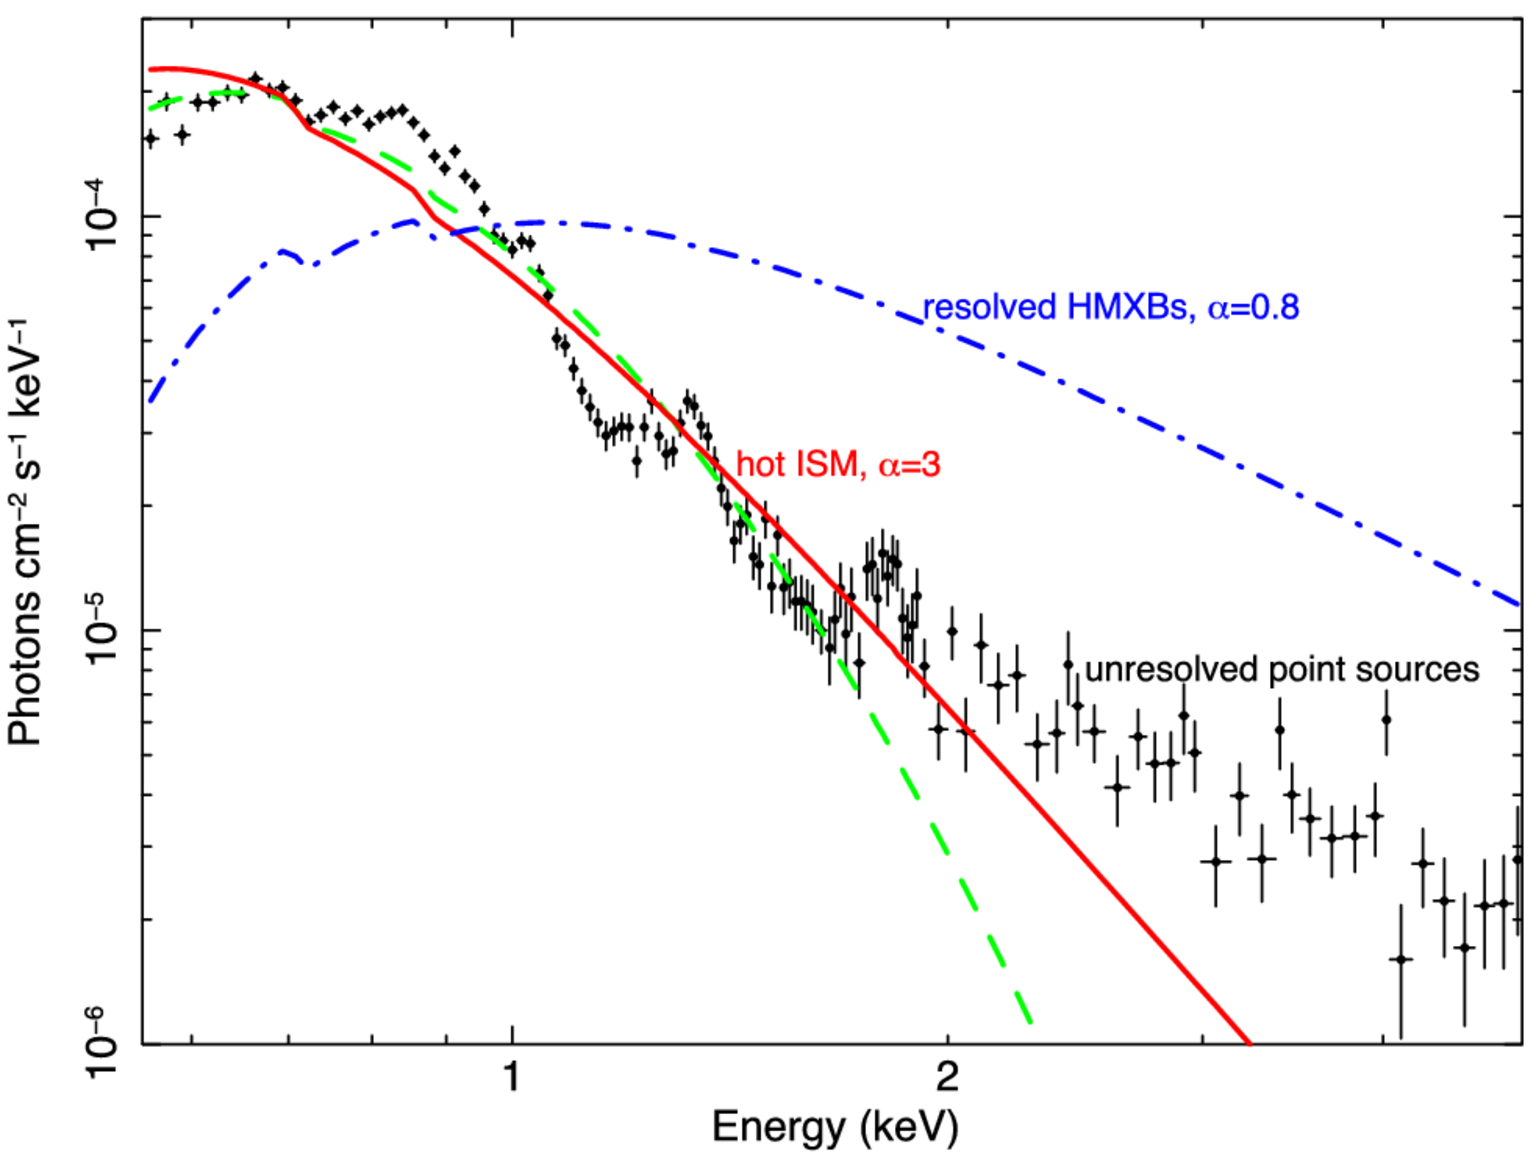
\includegraphics[width=0.49\textwidth]{Mirocha/pacucci2014_fig1.pdf}
\end{center}
\caption{{\bf Models for the X-ray spectra of star-forming galaxies.} \textit{Left:} Template Cygnus X-1 spectrum (solid) compared with power-law (dashed), with mean free path shown on left scale and relative luminosity on right \cite{Fialkov2014b}. \textit{Right:} Typical HMXB spectrum (blue) compared to soft X-ray spectrum characteristic of bremmstrahlung emission from hot ISM gas \cite{Pacucci2014}.}
\label{fig:xray_seds}
\end{figure*}


Though the soft X-ray luminosity from hot gas appears to be subdominant to the HMXB component in nearby galaxies, there are of course uncertainties in how these relations evolve. Furthermore, the bremmstrahlung emission characteristic of hot ISM gas has a much steeper $\sim \nu^{-2.5}$ spectrum than inverse Compton ($\sim \nu^{-1}$) or XRBs ($\sim \nu^{-1}$ or $\nu^{-1.5}$), and thus may heat more efficiently (owing to $\sigma \propto \nu^{-3}$ cross section) provided soft X-rays can escape galaxies. 

%%
% NHI, Emin
%%
\subsection{Escape of X-rays from Galaxies}
Though the mean free paths of X-rays are longer than those of UV photons, they still may not all escape from galaxies into the IGM. For example, hydrodynamical simulations suggest typical hydrogen column densities of $\NHI \sim 10^{21} \ \mathrm{cm}^{-2}$ in low-mass halos \cite{Das2017}, which is substantial enough to eliminate emission below $\sim 0.5$ keV. 

Given the many unknowns regarding X-ray emission in the early Universe, 21-cm models often employ a three-parameter approach, i.e., instead of a single value of $\zeta_X$, the specific X-ray luminosity is modeled as 
\begin{equation}
	L_{X,\nu} = L_{X,0} \left(\frac{h \nu}{1 \mathrm{keV}} \right)^{\alpha_X} \exp\left[-\sigma_{\nu} \NHI \right]
\end{equation}
and the normalization, $L_{X,0}$, spectral index $\alpha_X$, and typical column density, $\NHI$, are left as free parameters. 

It is common to approximate this intrinsic attenuation with a piecewise model for $L_X$, i.e., 
\begin{align}
L_{X,\nu} = \left\{ \begin{array}{cc} 
                0 & h\nu < \Emin \\
                L_{X,0} \left(\frac{h \nu}{1 \mathrm{keV}} \right)^{\alpha_X} & h\nu \geq \Emin \
                \end{array} \right.
\end{align}
Note that $\NHI$ (or $\Emin$) can be degenerate with the intrinsic spectrum, e.g., the SED of HMXBs in the high-soft state exhibits a turn-over at energies $h\nu < 1$ keV, which could be mistaken for strong intrinsic absorption.

{\color{red} Translate this to $\zeta_X$.}


% DCBHS? 
\subsection{Cosmic Rays from Supernovae}
{\color{red} Other sources of high energy radiation have been explored in recent years though are generally found to be sub-dominant. However, surprises may be in store...}

%%%
%% Modeling 
%%%
\section{Predictions for the 21-cm Background} \label{sec:predictions}
Over the last four sections we have assembled a simple physical picture of the IGM at high redshift and the sources most likely to affect its properties. Here, we finally describe the generic sequence of events predicted in most 21-cm models and the sensitivity of the 21-cm background to various model parameters of interest. 

%%
% Generic predictions
%%
\subsection{Generic Series of Events}
Figure \ref{fig:eosFG} shows an illustrative example including a 2-D slice of the $\delta T_b$ field, the global 21-cm signal, and power spectrum on two spatial scales. Time proceeds from right to left from $\sim 20$ Myr after the Big Bang until the end of reionization $\sim 1$ Gyr later.

\begin{figure*}[]
\begin{center}
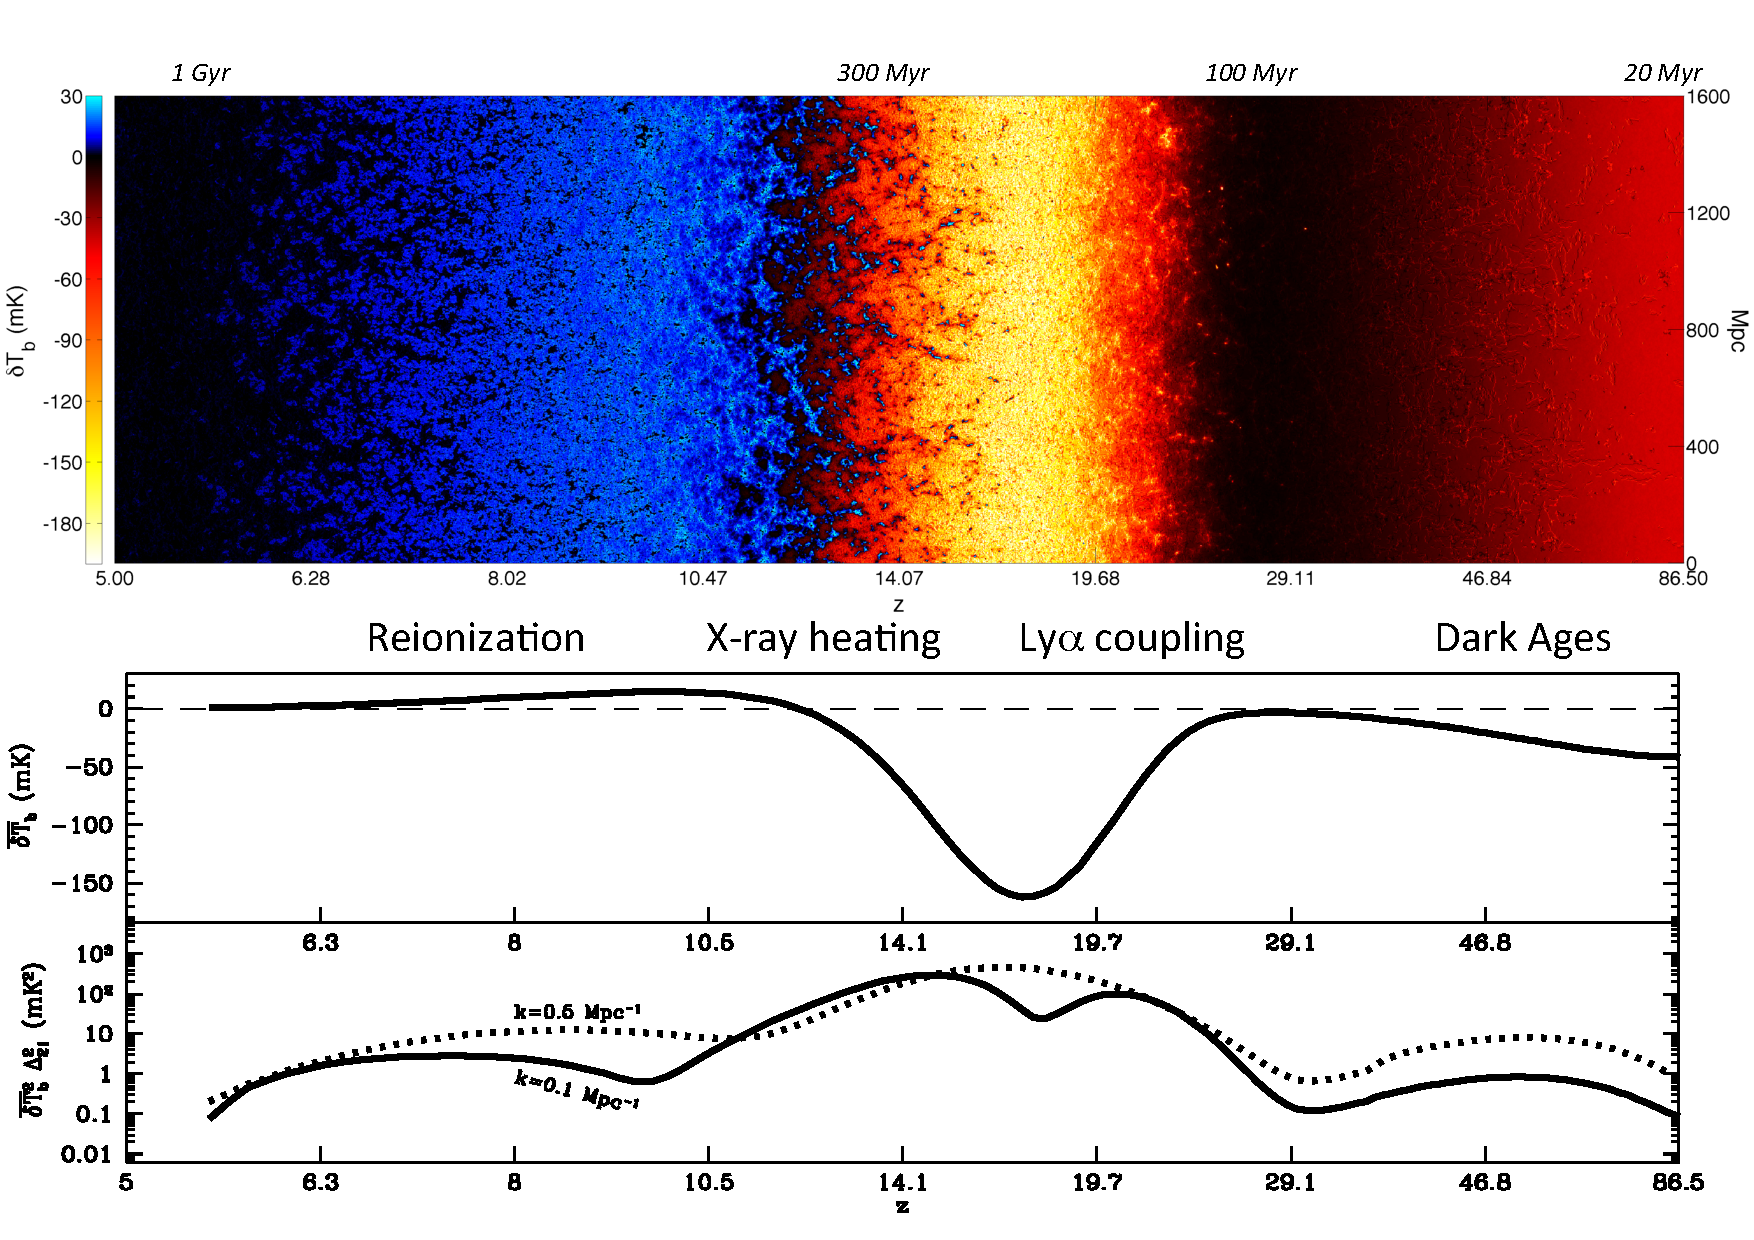
\includegraphics[width=0.98\textwidth]{Mirocha/eosFG.pdf}
\end{center}
\caption{{\bf Predictions from the \textsc{21cmfast} Evolution of Structure (EoS) model suite.} \textit{Top}: 2-D slice of the brightness temperature field, with red colors indicating a cool IGM, blue colors indicative of a heated IGM, and black representing a null signal (either due to ionization or $\TS=\Tcmb$). \textit{Middle:} Global 21-cm signal, with dashed line indicating  $\delta T_b = 0$. \textit{Bottom:} Evolution of the dimensionless 21-cm power spectrum, $\Delta^2 = k^3 P(k) / 2\pi^2$, on two different scales, $k=0.5 \ \mathrm{Mpc}^{-1}$ (dotted) and $k=0.1 \ \mathrm{Mpc}^{-1}$ (solid).}
\label{fig:eosFG}
\end{figure*}

There are four distinct epochs indicated within this time period, which we describe in more detail below.
\begin{description}
	\item[The Dark Ages:] As the Universe expands after cosmological recombination, Compton scattering between free electrons and photons keep the radiation and matter temperature in equilibrium. The density is high enough the collisional coupling remains effective, and so $\TS = \TK = \TCMB$. Eventually, Compton scattering becomes inefficient as the CMB cools and the density continues to fall, which allows the gas to cool faster than the CMB ({\color{red} see also Jonathan's chapter, Steve's chapter}). Collisional coupling remains effective for a short time longer and so $\TK$ follows $\TS$. This results in the first decoupling of $\TS$ from $\TCMB$ at $z \sim 80$, and thus an absorption signature at $\nu \sim 15$ MHz, which comes to an end as collisional coupling becomes inefficient, leaving $\TS$ to reflect $\TCMB$ once again.
	\item[Ly-$\alpha$ coupling:] When the first stars form they flood the IGM with UV photons for the first time. While Lyman continuum photons are trapped near sources, photons with energies $10.2 < h\nu / \mathrm{eV} < 13.6$ either redshift directly through the $\Lya$ resonance or cascade via higher $\Lyn$ levels, giving rise to a large-scale $\Lya$ background capable of triggeiring Wouthuysen-Field coupling as they scatter through the medium (see also \S\ref{sec:ch1_lya} and \S\ref{sec:lya_global}). As a result, $\TS$ is driven back toward $\TK$, which (in most models) still reflects the cold temperatures of an adiabatically-cooling IGM.
	\item[X-ray Heating:] The first generations of stars beget the first generations of X-ray sources, whether they be the explosions of the first stars themselves or remnant neutron stars or black holes that subsequently accrete. Though the details change depending on the identity of the first X-ray sources, generally such sources provide photons energetic enough to travel great distances. Upon absorption, they heat and partially ionize the gas, eventually driving $\TS > \TCMB$. Once $\TS \gg \TCMB$, the 21-cm signal ``saturates,'' and subsequently sensitive only to the density and ionization fields. However, it is possible that heating is never ``complete'' in this sense before the completion of reionization, meaning neutral pockets of IGM gas may remain at temperatures at or below $\TCMB$ until they are engulfed by overlappin ionized bubbles.
	\item[Reionization:] As the global star formation rate density climbs, the growth of ionized regions around groups and clusters of galaxies will continue, eventually culminating in the completion of cosmic reionization. This rise in ionization corresponds to a decline in the amount of neutral hydrogen in the Universe capable of producing or absorbing 21-cm radiation. As a result, the amplitude of the 21-cm signal, both in its mean and fluctuations, falls as reionization progresses.
\end{description}

This particular model \cite{Mesinger2016} assumes that very faint galaxies dominate the UV and X-ray emissivity, which results in relatively early features in the 21-cm background, e.g., both the power spectrum and global 21-cm signal peak in amplitude at $z \sim 18$. Reionization and reheating occur later in scenarios in which more massive halos dominate the emissivity, and may even overlap, resulting in strong 21-cm signals at $z \lesssim 12$ \cite{Mesinger2016,Mirocha2017,Park2019}. 

For the remainder of this section we focus on changes in the 21-cm signal wrought by parameters of interest. We limit our discussion to the global 21-cm signal and power spectrum, though there are of course many other statistics one could use to constrain model parameters (see Chapter 3).


%%
% Parameter studies
%%
\subsection{Sensitivity to Model Parameters}
There is no consensus parameterization for models of galaxy formation or the 21-cm background, nor do all models incorporate the same physical processes or employ the same numerical techniques. As a result, in this section we make no effort to closely compare or homogenize results from the literature, but instead draw examples from many works in order to illustrate different aspects of the 21-cm background as a probe of galaxy formation.


\subsubsection{The Minimum Mass}
The minimum mass (or equivalent virial temperature) for star formation sets the total number of halos emitting UV and X-ray photons as a function of redshift. Fiducial models often adopt the mass corresponding to a virial temperature of $10^4$ K, since gas in halos of this mass will be able to cool atomically, i.e., there is not an obvious barrier to star formation in halos of this mass. Reducing $\mmin$, as is justified if star formation in minihalos is efficient, results in a larger halo population, while increasing $\mmin$ of course reduces the halo population. It is very possible that $\mmin$ evolves with time, capturing first the epoch in which minihalos dominate the luminosity density of the Universe, then atomic cooling halos, and finally halos still massive enough to withstand reionization feedback ({\color{red} references}).

As shown in Figure \ref{fig:mesinger2014_fig3}, $\mmin$ affects all features of the 21-cm background, both in the global signal and fluctuations, because it changes the total number of halos emitting at all wavelengths.

 
\begin{figure*}[]
\begin{center}
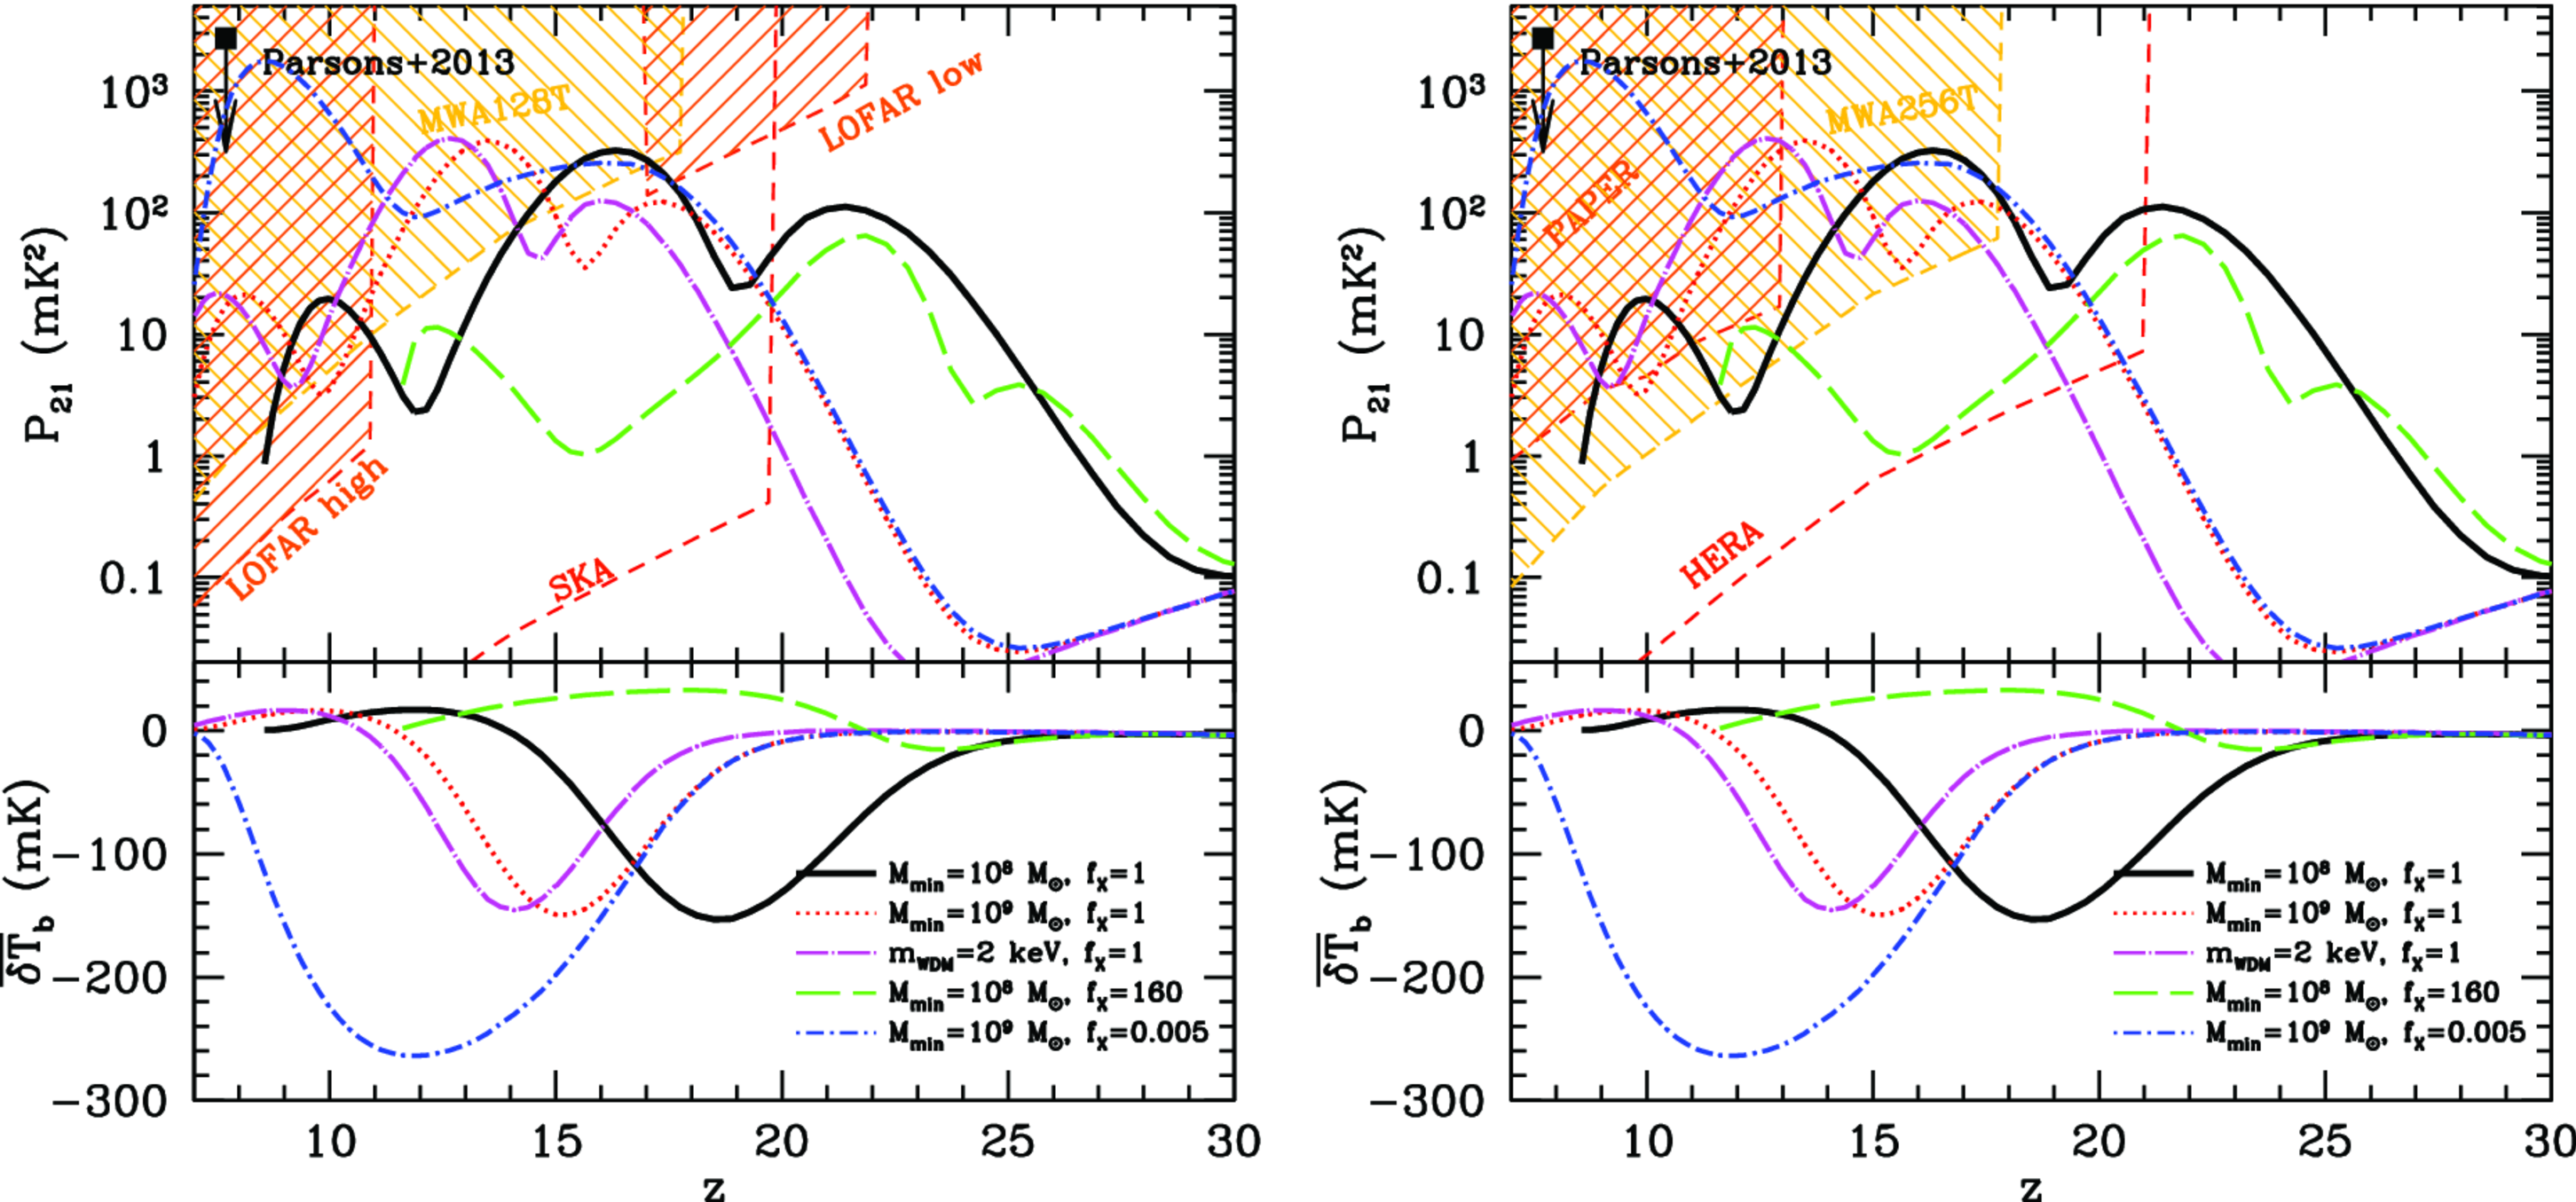
\includegraphics[width=0.98\textwidth]{Mirocha/mesinger2014_fig3.pdf}
\end{center}
\caption{{\bf Effects of the minimum mass on the global 21-cm signal and 21-cm power spectrum on $k=0.1 \ \mathrm{Mpc}^{-1}$ scales \cite{Mesinger2014}.}}
\label{fig:mesinger2014_fig3}
\end{figure*}

\subsubsection{The Ionizing Efficiency}
Generally written as $\zeta$ or $\zetaI$, the ionizing efficiency quantifes the number of Lyman continuum (LyC) photons that are produce in galaxies and escape into the IGM. As a result, this parameter affects primarily the lowest redshifts (highest frequencies), as can be seen in Figure XYZ. In the global 21-cm signal, $\zetaI$ dictates the rate at which the signal decays to zero, while in the power spectrum, $\zetaI$ controls the redshift at which the fluctuations peak.

{\color{red} Is there a good figure for this?}

\subsubsection{The X-ray Efficiency and Spectrum}
Show Jonathan's fX-fa plot Fig. \ref{fig:p12_fafX}, \ref{fig:xsed_ps}. See also, \cite{Mirabel2011,Mirocha2014}.

\begin{figure*}[]
\begin{center}
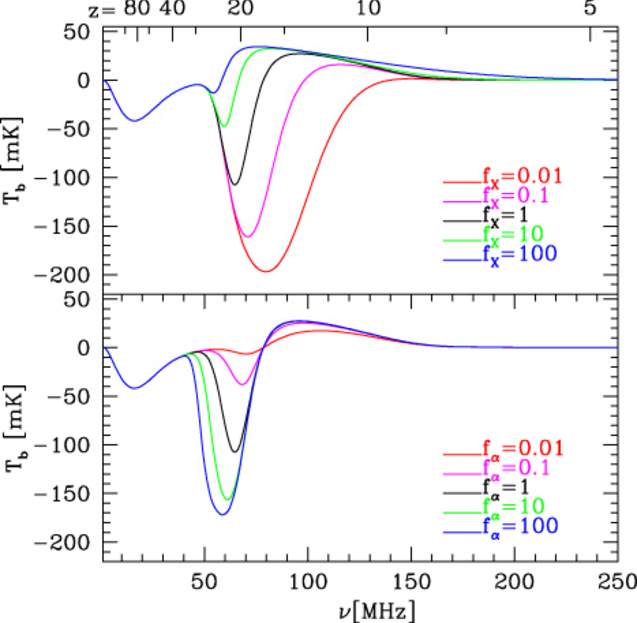
\includegraphics[width=0.49\textwidth]{Mirocha/pritchard2012_fafX.pdf}
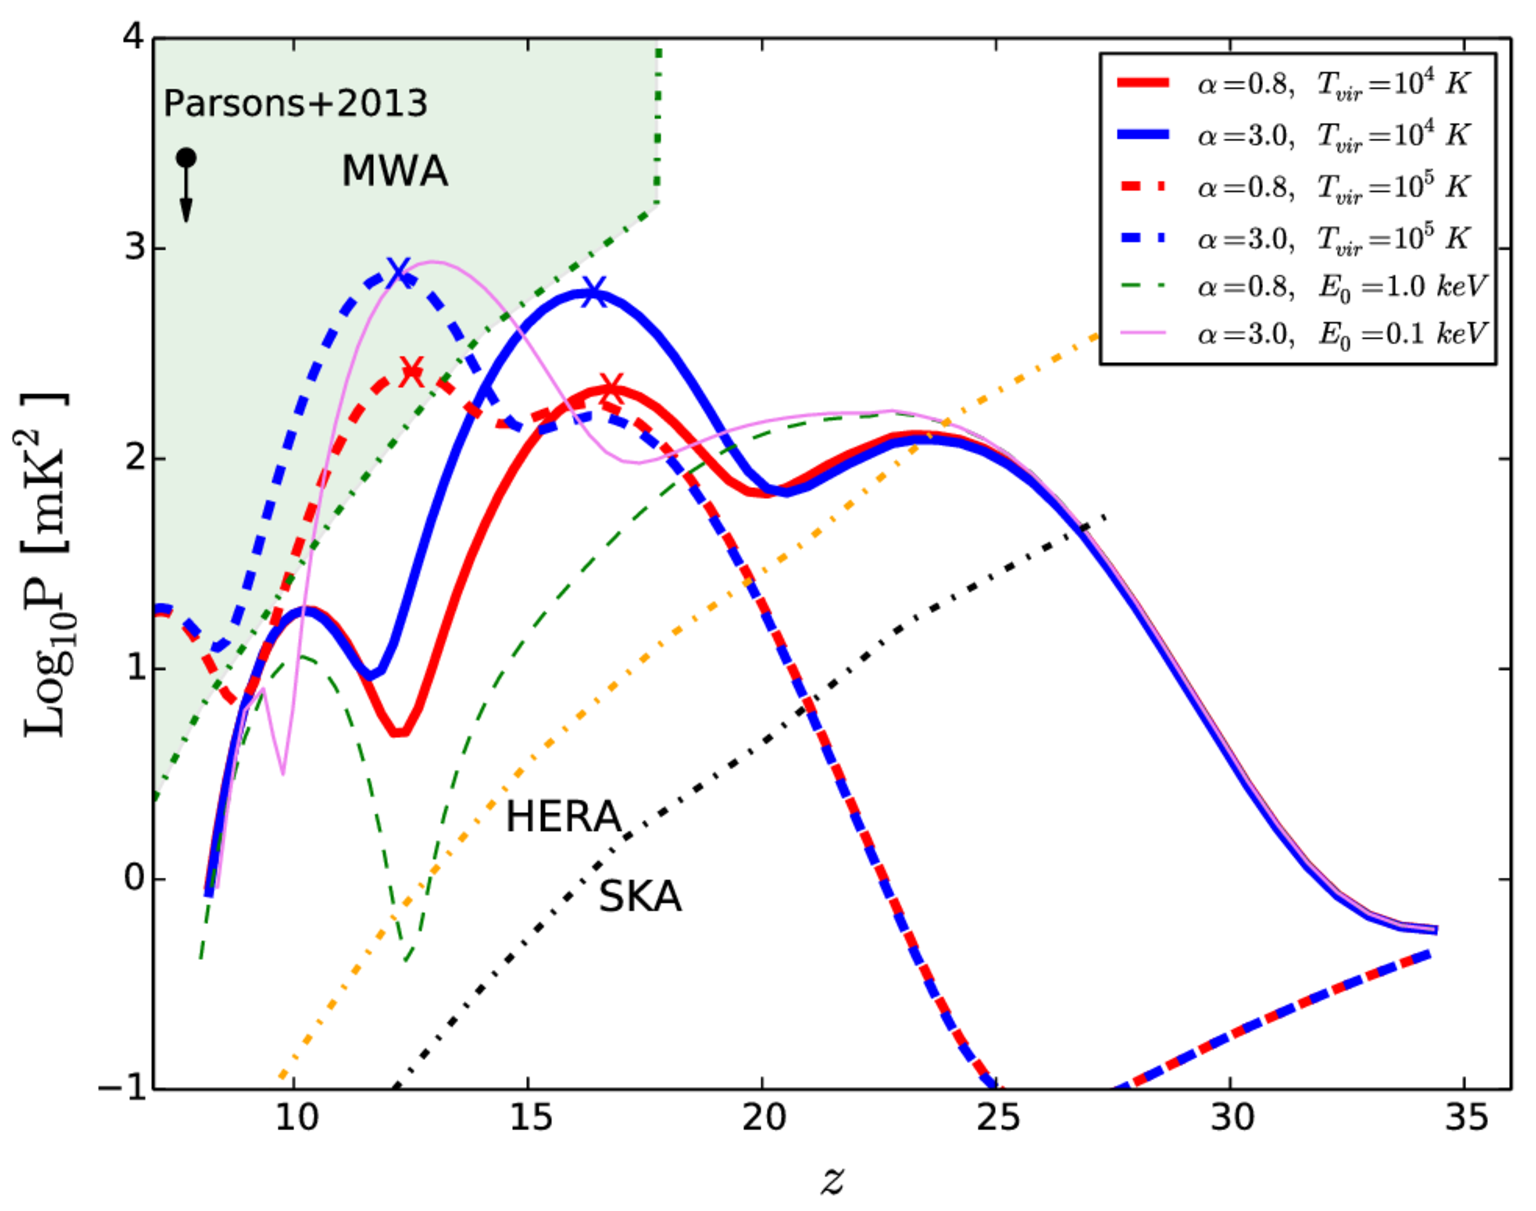
\includegraphics[width=0.49\textwidth]{Mirocha/pacucci2014_fig5.pdf}
\end{center}
\caption{{\bf Effects of $\Lya$ and X-ray efficiencies on the global 21-cm signal \cite{Pritchard2010,Pacucci2014}.} \textit{Left:} Predictions for the global 21-cm signal showing sensitivity to the normalization of the $L_X$-SFR relation, $f_X$ (top), and the production efficiency of $\Lya$ photons, $f_{\alpha}$ (bottom) \cite{Pritchard2010}. \textit{Right:} Predictions for evolution in the 21-cm power spectrum at $k=0.2 \ \mathrm{Mpc}^{-1}$ for models with different X-ray spectra \cite{Pacucci2014}. Blue curves indicate soft power-law spectra with indices of $\alpha=3$, while red curves are indicative of hard spectra sources with $\alpha=0.8$. Linestyles denote different minimum virial temperatures, $\Tmin$, and lower energy cutoffs for the X-ray background, $E_0$.}
\label{fig:p12_fafX}
\end{figure*}



\subsubsection{The Ly-$\alpha$ Efficiency}
The production efficiency of $\Lya$ photons primarily affects when the 21-cm background first ``turns on.'' 

{\color{red} Fig. \ref{fig:p12_fafX}. Figure from BL05?}


\subsubsection{Synthesis Models}
It is common to allow $\zeta$, $\zeta_X$, and $\zeta_{\alpha}$ to vary independently as free parameters. However, if all features of the 21-cm background are driven by stars and their remnants, and the properties of such objects do not vary with time, then these efficiency factors will be highly correlated. For example, the number of Lyman continuum photons produced per unit star formation is inversely proportional to stellar metallicity, as is the yield in the Lyman Werner band, so it may be more appropriate to use $Z_{\ast}$ as the free parameter, rather than $\Nion$ and $\Nlw$. It is harder to justify connecting $N_X$ to $Z_{\ast}$ as it depends on the poorly understood details of stellar (and compact remnant) evolution. However, observationally the $L_X$-SFR relation appears to depend on gas-phase metallicity \cite{Brorby2016}. 

Figure \ref{fig:gs_metallicity} shows these effects on the global 21-cm signal \cite{Mirocha2017}. {\color{red} Note little evolution without X-ray dependence since calibrating to LFs.}

\begin{figure*}[]
\begin{center}
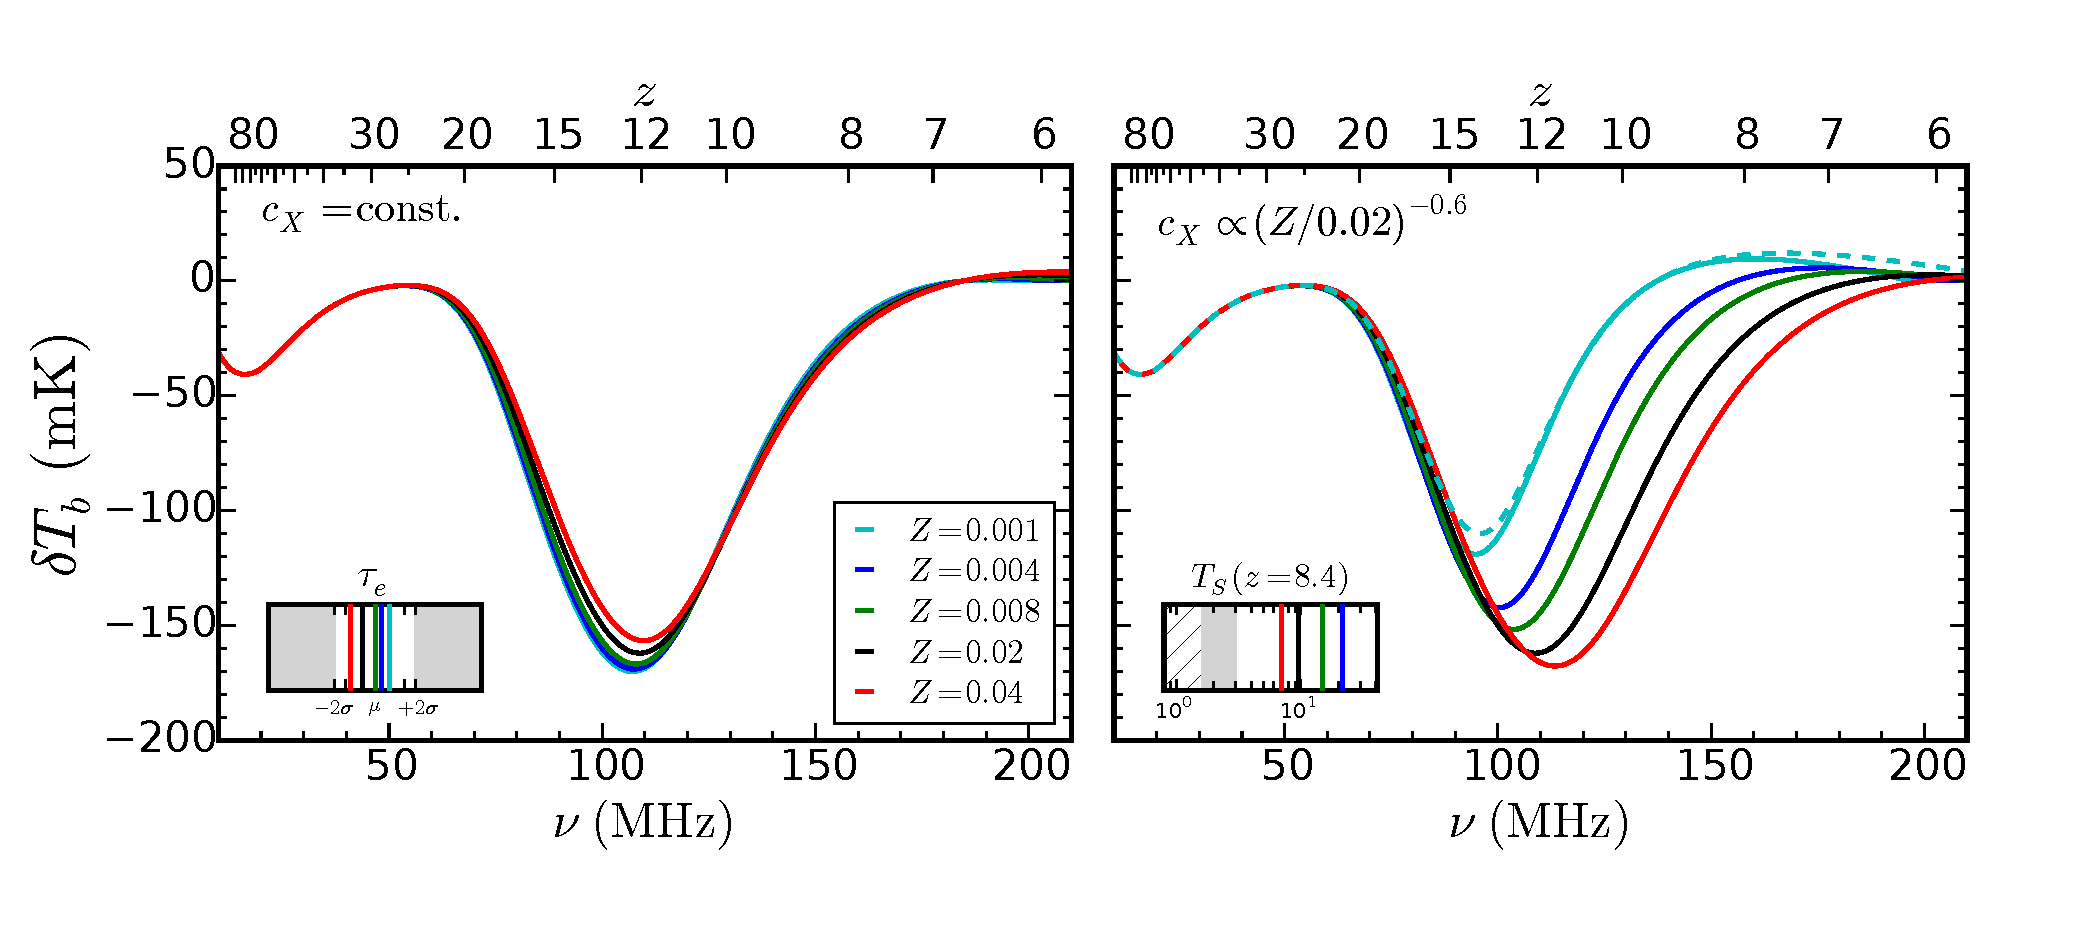
\includegraphics[width=0.98\textwidth]{Mirocha/mirocha2017_fig5.pdf}
\end{center}
\caption{{\bf Effects of stellar metallicity on the global 21-cm signal \cite{Mirocha2017}.}}
\label{fig:gs_metallicity}
\end{figure*}


% LW Feedback
\subsubsection{Feedback Effects}
The strength of feedback can also alter the timeline of events in the 21-cm background. Particularly at early times, LW feedback modifies the minimum mass, and thus, the strength of the UV background, as shown in Figure \ref{fig:LWfeedback}.

\begin{figure*}[]
\begin{center}
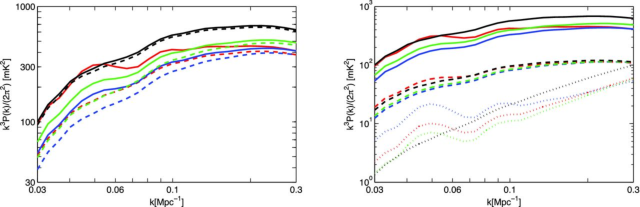
\includegraphics[width=0.98\textwidth]{Mirocha/fialkov2014_fig6.pdf}
\end{center}
\caption{{\bf Effects of LW feedback on the 21-cm power spectrum \cite{Fialkov2013}.} The strength of the feedback is indicated by different colors -- no feedback (red), weak (blue), strong (green), and saturated (black) In the left panel, dashed curves exclude the baryon-DM velocity offset effect \cite{Tseliakovich2010}, while in the right panel, all models include this effect, and linestyles indicate power spectra at three different redshifts.}
\label{fig:LWfeedback}
\end{figure*}



%\begin{center}
%\begin{table}
%\begin{tabular}{||c | c | c||}
%\hline
%name & description & typical values \\ 
%\hline\hline
%$\zeta_i$ & Ionizing photon production efficiency & 40 ish  \\ 
%\hline
%$\zeta_{\alpha}$ & $\Lya$ photon production efficiency & 40 ish  \\ 
%\hline
%$\zeta_X$ & X-ray photon production efficiency & xxx \\
%\hline
%$\Tmin$ & Minimum virial temperature of star-forming halos & $10^4$ K \\
%\hline
%\end{tabular}
%\caption{Parameters in simple 21-cm models.}
%\end{table}
%\end{center}
%
\subsubsection{Pop~III v. Pop~II}
Figure \ref{fig:popIII_gs}

\begin{figure*}[]
\begin{center}
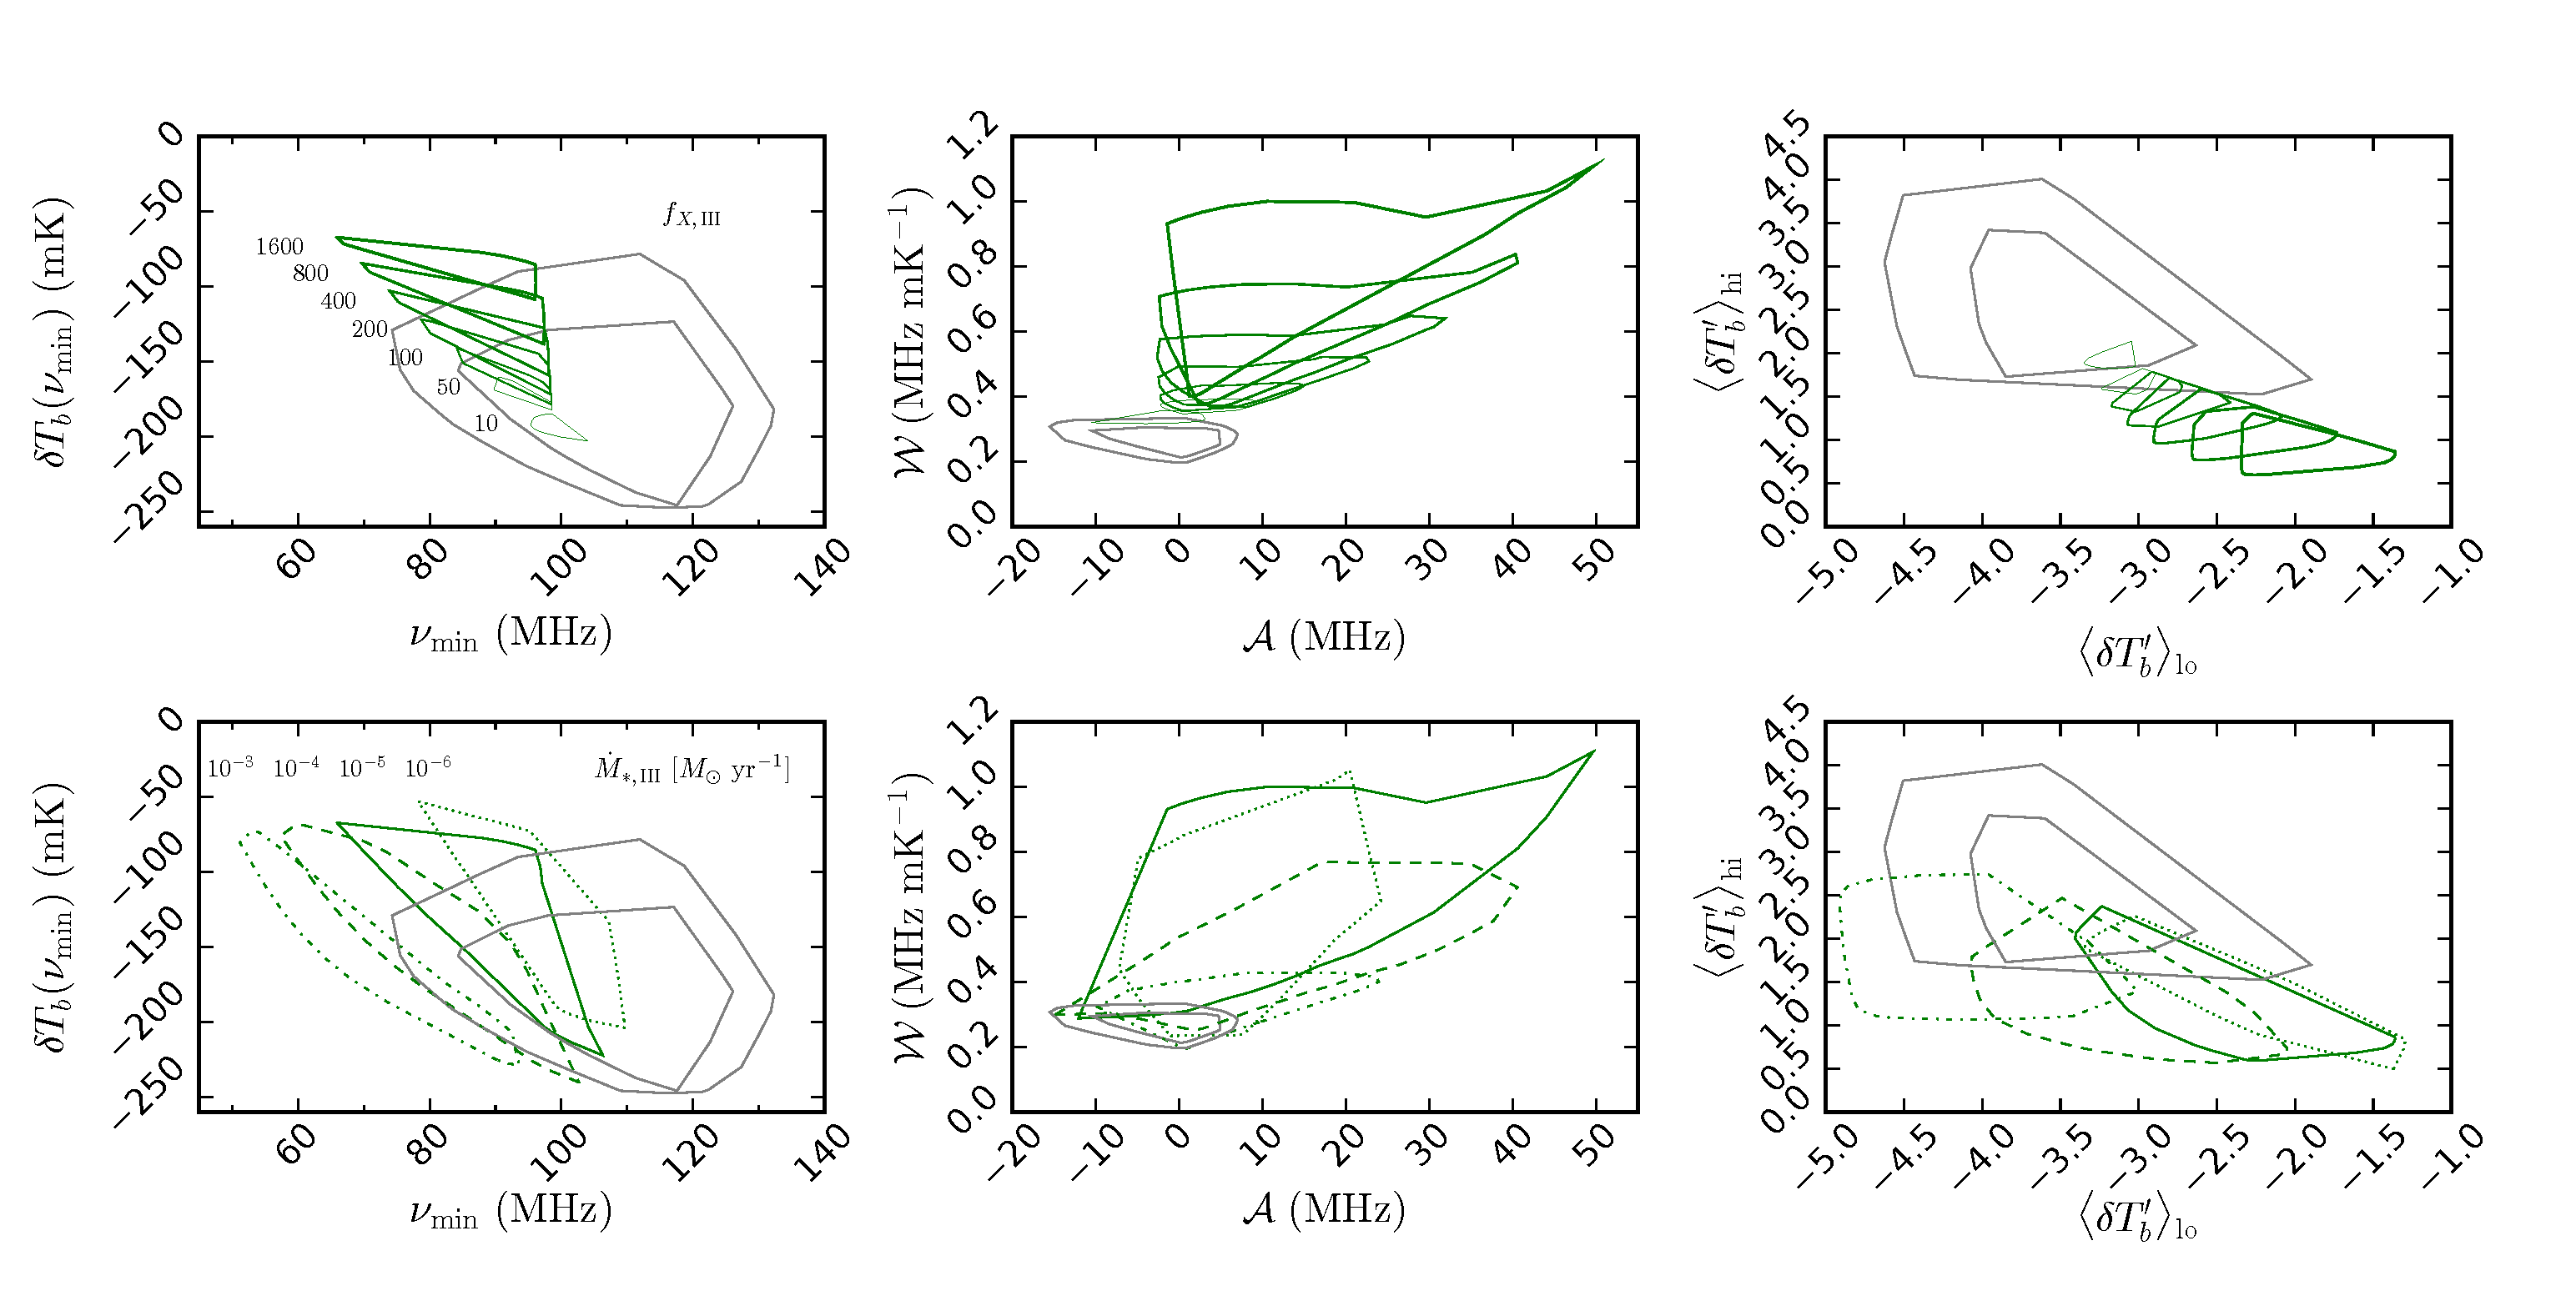
\includegraphics[width=0.98\textwidth]{Mirocha/mirocha2018_fig6.pdf}
\end{center}
\caption{{\bf Potential PopIII signatures.}}
\label{fig:popIII_gs}
\end{figure*}


%%
% TOOLS
%%
\subsection{Modeling Tools} \label{sec:codes}
Predictions from previous section came from a mix of different groups and codes. Discuss some differences here.

Codes to include:
\begin{itemize}
	\item \textsc{21cmFAST} and \textsc{DexM}
	\item Anastasia's code
	\item \textsc{simfast21}
	\item \textsc{ares}	
	\item RT simulations: C2ray, ramses, enzo,...
\end{itemize}


\bibliographystyle{plain}
\bibliography{Mirocha/References}



%\chapter{Physical cosmology from the 21-cm line}

\begin{bf}
  \author{Jonathan Pritchard}\\
  
a discussion of using 21-cm intensity mapping/interferometry to constrain the matter power spectrum and cosmological parameters.  The signal can also be used as a signpost for new physics beyond the standard model, such as heating and cooling of the primordial gas through interactions with dark matter.  Subtopics could include: redshift space distortions and their likely observability, measuring the matter power spectrum during the cosmic dawn and (eventually) the dark ages, IGM heating through dark matter annihilations, IGM cooling through interactions with exotic dark matter candidates.  \\
\end{bf}

This chapter discusses some important things

\section{Physical cosmology through the 21-cm epoch}
Summarise the different ways in which cosmology underpins the nature of the 21 cm signal.

\subsection{Dark matter} 
Discuss different dark matter models and impact

\subsection{PMBH}
Discuss primordial black holes and other exotic objects 

%%%%%
\section{Unique signatures of cosmology}
What might be distinctive signatures of cosmology in the 21cm signal?

\subsection{Non-Gaussianity} 
Impact of clustering on bubbles.

\subsection{IGM Heating} 
Various ways exotic physics can impact 21 cm signal

%%%%%
\section{Separating cosmology from astrophysics}
How might cosmology be separated from astrophysics?

\subsection{Redshift space distortions}
As route to separating different elements of signal

\subsection{Time evolution}
Looking at the dark ages, or via time evolution, or going to late times to post-EoR.

\section{Summary}

Lorem ipsum dolor sit amet, consectetur adipiscing elit. Duis eu egestas erat. Maecenas tincidunt lacinia tincidunt. Mauris id lectus nec neque feugiat condimentum vitae at diam. In vel orci nunc, non commodo mauris. Vivamus ipsum enim, vulputate quis pharetra non, molestie quis felis. Vivamus porttitor placerat turpis at accumsan. Nunc tortor velit, faucibus a rhoncus nec, blandit non elit. Nam consectetur lectus eu nisi blandit dapibus rhoncus dui tempus. Mauris fermentum dolor vel ipsum vulputate sit amet ultricies tortor lacinia. Donec ut nibh erat. Morbi nec mi ante. Integer nec vestibulum diam. Donec tincidunt pellentesque quam, ut interdum mauris venenatis condimentum. Nam condimentum, augue in aliquet gravida, neque dui elementum eros, id semper eros purus sed felis. Curabitur in justo sit amet sapien ultrices hendrerit at quis nibh. Quisque iaculis pulvinar tincidunt. 
\begin{eqnarray}
C(12) &= &\left[\overrightarrow{\pi}\cdot\overrightarrow{\phi}(x+r)\right] \nonumber \\ 
&\approx& 1-\mathrm{const}\frac{r^2}{L^2}\int_r^L\frac{x\rmd x}{x^2} + \cdots \nonumber  \\
&\approx& 1-\mathrm{const}\frac{r^2}{L^2}\ln\frac{x\rmd x}{x^2} + \cdots .\label{brokenlongeqn}
\end{eqnarray}

Aenean tellus risus, porta sit amet porta vitae, tincidunt ut felis. Class aptent taciti sociosqu ad litora torquent per conubia nostra, per inceptos himenaeos. Vestibulum ante ipsum primis in faucibus orci luctus et ultrices posuere cubilia Curae; Phasellus pulvinar placerat velit auctor egestas. Vivamus euismod fringilla tincidunt. Sed ut magna felis, id sollicitudin nunc. Quisque a dui eu erat consectetur egestas a quis justo. Aenean euismod congue diam, vel posuere urna fermentum sit amet. Lorem ipsum dolor sit amet, consectetur adipiscing elit. Mauris faucibus lacus eget est mollis auctor. Donec at nibh ligula, et posuere massa. Phasellus quis leo diam \cite{diamantaras1996pcn}.
Donec aliquam blandit risus, eu venenatis ante euismod eu. Curabitur cursus justo id arcu condimentum feugiat. Integer sapien urna, vulputate et adipiscing nec, convallis et justo. Suspendisse in ipsum at felis ornare interdum \cite{tulone2006pts},

\begin{figure}[]
\begin{center}

\includegraphics[width=0.5\textwidth]{Mirocha/01x01-eps-converted-to}
\end{center}
\caption{This is figure 1 in chapter 1.}
\end{figure}

\paragraph{Cras adipiscing} sagittis nunc vel luctus. Suspendisse volutpat augue quis erat semper consequat dignissim tellus euismod. Morbi hendrerit, tellus id aliquam iaculis, nibh leo tincidunt eros, vitae varius ligula felis in mi.

\begin{table}
\caption{Greek Letters.}
\begin{center}
\begin{tabular}{llllllll}
\hline
$\alpha $  & $ \beta $  & $ \gamma $  & $ \delta $  & $ \epsilon $  & $ \varepsilon $  & $ \zeta $  & $ \eta $ \\
 $ \theta $  &  $ \vartheta $  &  $ \gamma $  &  $ \kappa $  &  $ \lambda $  &  $ \mu $  &  $ \nu $  &  $ \xi $ \\
 $ o $  &  $ \pi $  &  $ \varpi $  &  $ \rho $  &  $ \varrho $  &  $ \sigma $  &  $ \varsigma $  &  $$ \\
 $ \tau $  &  $ \upsilon $  &  $ \phi$ &  $ \varphi $  &  $ \chi $  &  $ \psi $  &  $ \omega$  &  $ $ \\
 &  &  &  &  &  &  & \\
$ \Gamma $  & $ \Delta $  & $ \Theta $  &  $ \Lambda $  &  $ \Xi $  &  $ \Pi $  &  $ \Sigma $  & $ \Upsilon $ \\
 $ \Phi$ &  $ \Psi $  &  $ \Omega $  &  &  &  &  &\\
\hline
\end{tabular}
\end{center}\end{table}

\begin{figure}[]
\begin{center}

\includegraphics[width=0.6\textwidth]{Mirocha/01x02}
\end{center}
\caption{This is figure 2 in chapter 1.}
\end{figure}


\bibliographystyle{plain}
\bibliography{Mirocha/References}



%\chapter{Inference from the 21cm signal}

\begin{bf}
  \author{Bradley Greig}\\
  
Abstract\\
\end{bf}

In the previous chapters we have discussed in-depth the astrophysical and cosmological information that is encoded by the cosmic 21-cm signal. However, once we have a measurement, how do we extract this information from the signal? This chapter focusses on the inference of the interesting astrophysics and cosmology once we obtain a detection of the 21-cm signal. 

Essentially, inference of the astrophysics can be broken down into three parts:
\begin{itemize}
\item[1.] \textbf{Characterisation of the observed data:} The observed 21-cm signal varies spatially as well as along the line-of-sight (frequency or redshift dimension) to provide a full three dimensional movie of the intergalactic medium in the early Universe. However, we cannot perform a full pixel-by-pixel comparison between theoretical models and the observed signal. Instead, we require a variety of statistical methods to average the observational data in order to be able to better characterise and compare the behaviour of the faint signal. 
\item[2.] \textbf{An efficient method to model the 21-cm signal:} In order to interpret the observations and understand the astrophysical processes responsible, we must be able to produce physically motivated models capable of replicating the signal. Further, these must be as computationally efficient as possible in order to be able to realistically investigate the 21-cm signal.
\item[3.] \textbf{A robust probabilistic framework to extract the physics:} The observed 21-cm signal is dependent on numerous physical processes, which within our models or simulations are described by many unknown parameters. Further, these contain approximations in order to deal with the requisite dynamic range. We must be able to characterise our ignorance in a meaningful way in order to be truly able to infer the astrophysical processes of the epoch of reionisation and cosmic dawn.
\end{itemize}
\noindent
In this chapter we will focus on each separately, discussing the current state-of-the-art in inferring astrophysical and cosmological information from the 21cm signal.

\section{What do we actually measure?}

The 21-cm signal from the neutral hydrogen in the intergalactic medium is measured by its brightness temperature, $T_{\rm b}$. However, this cannot be measured directly, instead it is expressed as a brightness temperature contrast, $\delta T_{b}$, relative to the Cosmic Microwave Background (CMB) temperature, $T_{\rm CMB}$ \cite{Furlanetto:2006a}: 
\begin{equation} \label{eq:delTb}
\delta T_{b}(\mathbf{x},\nu) \equiv T_{\rm b}(\mathbf{x},\nu) - T_{\rm CMB, 0}.
\end{equation}
As such, this brightness temperature contrast can be seen either in emission or absorption, dependent on the 21-cm brightness temperature which itself is dependent on the excitation state of the neutral hydrogen (i.e. its spin temperature, $T_{\rm S}$, see Section~\ref{spin-temp}). We can re-express Equation~\ref{eq:delTb} in terms of $T_{\rm S}$ to recover,
\begin{equation} \label{eq:delTb_Ts}
\delta T_{b}(\mathbf{x},\nu) \equiv \frac{T_{\rm S}(\mathbf{x},\nu) - T_{\rm CMB}(z)}{1+z} \left( 1 - {\rm e}^{-\tau_{\nu_{0}}(\mathbf{x},\nu) } \right),
\end{equation}
where $\tau_{\nu_{0}}$ is the optical depth of the 21-cm line (see e.g. Section~\ref{rt-21cm}). $\delta T_{b}(\mathbf{x},\nu)$ varies spatially due to its two-dimensional angular position on the sky while it varies along the line-of-sight direction owing to the 21-cm line being redshifted by cosmological expansion (i.e. adding a frequency or time dependence to the signal). Thus, measuring $\delta T_{b}(\mathbf{x},\nu)$ can reveal a full three-dimensional movie of the neutral hydrogen in the early Universe.

Unfortunately, $\delta T_{b}(\mathbf{x},\nu)$ is faint. Further, in reality it is buried under numerous astrophysical foregrounds all of which are orders of magnitude brighter (see e.g. Chapter~6). In order to deal with this faint signal coupled with the astrophysical foregrounds, typically we seek to compress the data to boost the signal-to-noise or specifically tailor methods to extract the faint signal. In Section~\ref{sec:methods}, we will discuss the numerous methods proposed in order to tease out the faint astrophysical signal from the noise.

\section{Optimal methods for characterising the 21-cm signal} \label{sec:methods}

The first step in our efforts to be able to infer information about the astrophysical processes responsible for reionisation and the cosmic dawn is to explore optimal methods to characterise the 21-cm signal. In this section, we summarise the wide variety of approaches considered in the literature, highlighting the leverage that each is able to provide with respect to the underlying astrophysical processes. Note that throughout this chapter, all investigations into detecting the 21-cm signal are generated theoretically, either analytically or numerically. Thus, we urge the reader to refer to the corresponding references in order to understand the limiting assumptions.

\subsection{Global signal} \label{sec:global}

The simplest way to deal with such a faint signal is to average it over as large a volume as possible. Since the 21-cm signal is visible across the entire sky, one can produce a complete sky-averaged (global) 21-cm brightness temperature as a function of frequency (redshift). 

Although the two-dimensional spatial information from the 21-cm signal is lost, the main advantage is that it is relatively cheap to observe, requiring comparatively simple instrumentation (see e.g. Section 8.3). For example, a single radio dipole is capable of seeing essentially the entire sky at any one time, which has formed the basis for several single dipole experiments to measure the 21-cm signal. In Figure~\ref{fig:global}, we show a representative model of the global 21-cm signal, highlighting the major cosmological milestones that have been discussed in previous chapters. Thus, in each frequency bin, we measure an all-sky average of the 21-cm brightness temperature.

\begin{figure}[]
\begin{center}
%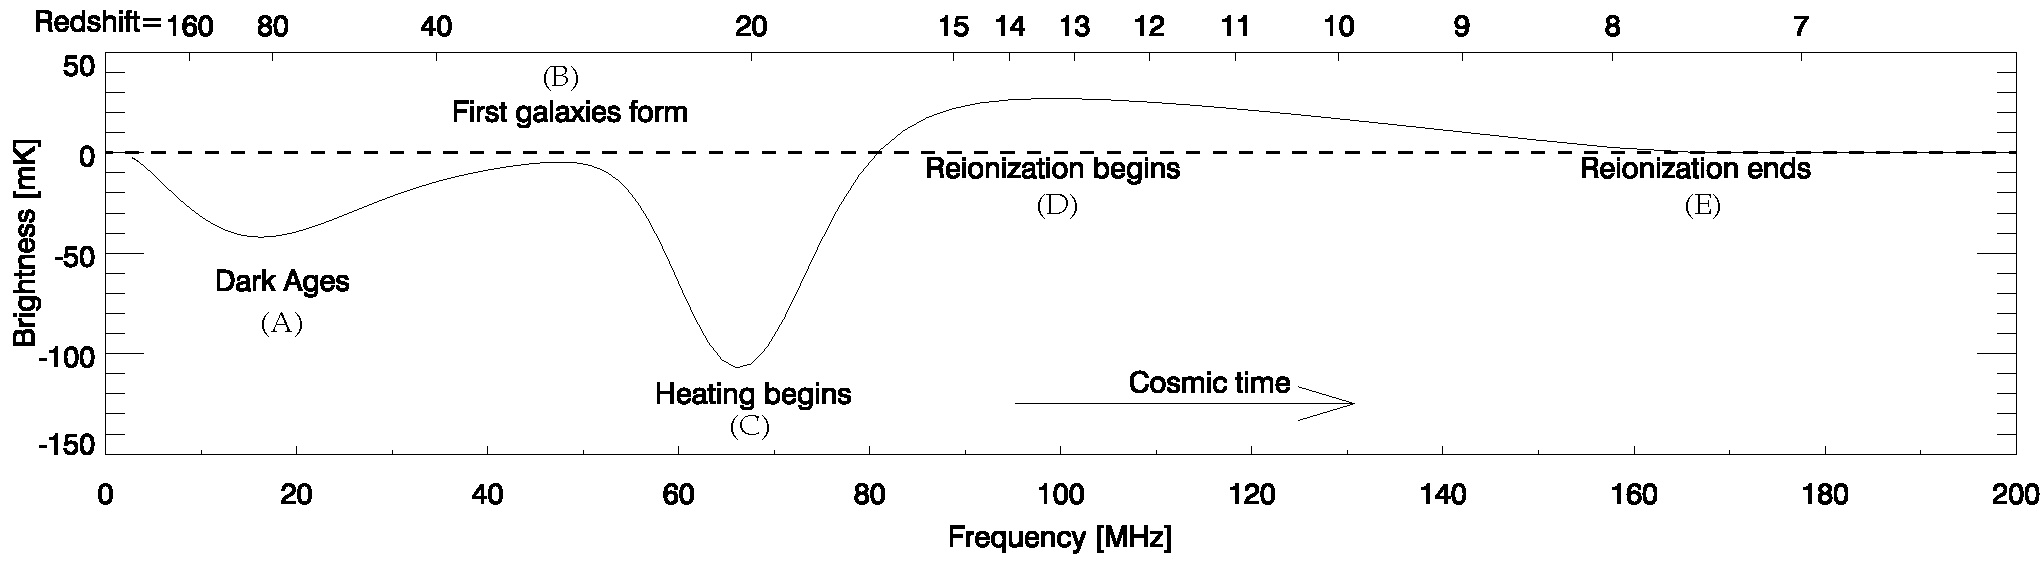
\includegraphics[width=1.\textwidth]{Greig/GlobalSignal}
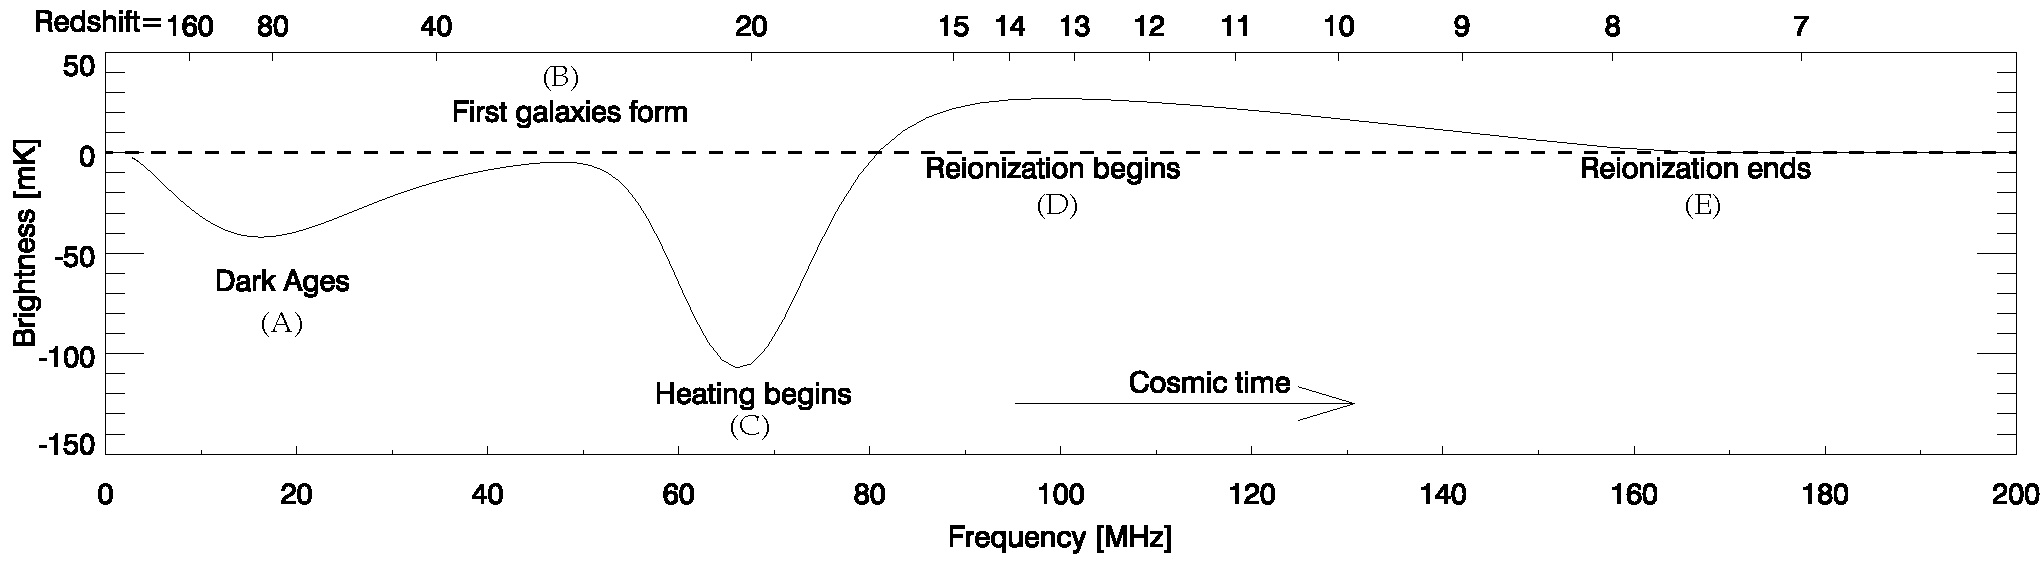
\includegraphics[trim = 0.2cm 0.6cm 0.2cm 0.2cm, scale = 0.45]{Greig/GlobalSignal}
\end{center}
\caption{A representative example of the all-sky averaged (global) 21-cm brightness temperature signal, demarcating the major cosmological transitions. Reproduced from \cite{Pritchard:2012}. \textcopyright IOP Publishing Ltd. All rights reserved.}
\label{fig:global}
\end{figure}

The global signal has been studied extensively in the literature (see e.g. \cite{Furlanetto:2006c,Pritchard:2010a,Pritchard:2012,Mirocha:2013,Fialkov:2014,Mirocha:2014,Mirocha:2015,Mirocha:2017,Cohen:2017,Fialkov:2018,Mirocha:2018,Fialkov:2019b}. Roughly speaking, the global 21-cm signal can be broken up into five major turning points (e.g. \cite{Furlanetto:2006b,Pritchard:2010a}) corresponding to: (A) a minimum during the dark ages where collisional coupling becomes ineffective, (B) a maximum at the transition from the dark ages to the Ly$\alpha$ pumping regime (Ly$\alpha$ pumping from the first sources becomes efficient), (C) a minimum at the commencement of X-ray heating taking the signal back towards emission, (D) a maximum once the 21-cm signal becomes saturated during the EoR and finally (E) when reionisation is complete. Importantly, both the amplitude of the 21-cm signal as well as the frequency (redshift) of these transitions is strongly dependent on the underlying astrophysical processes. Thus, measuring both the amplitude and frequency of the turning points can reveal information into the underlying astrophysics.

The second turning point (end of the dark ages) can, under certain simple assumptions, be used to place limits on the spin temperature, $T_{\rm S}$. Details on $T_{\rm S}$, through equations~\ref{eq:Ts}-\ref{eq:xalpha} can provide an estimate on the overall amplitude of the angle-averaged intensity of Ly$\alpha$ photons, $J_{\alpha}$. 
The relative depth of the third turning point (heating epoch) can be used to place limits on the co-moving heating rate density, that is, the amount of heating that the IGM has undergone owing to heating sources (e.g. X-rays from HMXBs, the ISM or other more exotic scenarios. See e.g. Sections 1.3 and~\ref{sec:sources} for further details). Finally, if the spin temperature saturates ($T_{\rm S} >> T_{\rm CMB}$) during the epoch of reionisation then the expression for the brightness temperature (Equation~\ref{eq:dtb}) collapses into an approximate proportionality ($T_{\rm S} \propto x_{\rm H{\scriptstyle I}}(1+\delta_{\rm nl})$) with the underlying ionisation fraction, $x_{\rm H{\scriptstyle I}}$. Tracking the evolution of the ionised fraction, i.e. the reionisation history, reveals the time-span of reionisation and the number density of ionising photons produced. 

Unfortunately, the estimates for the amplitude of the ionising, Lyman-$\alpha$ and X-ray backgrounds from the global signal cannot directly reveal insights into the population of sources responsible (e.g. their typical emission spectra) as these amplitudes are convolved with the underlying galaxy number density. In compressing the entirety of the signal down into these five turning points we cannot separate out the two contributions. However, this degeneracy can be broken when further spatial information is used (e.g the 21cm power spectrum; Section~\ref{sec:PS}).

To highlight the expected variation in the global 21-cm signal as a result of the underlying astrophysical processes, in Figure~\ref{fig:global_vary} we show $\sim~200$ theoretical models of the global 21-cm signal from \cite{Cohen:2017}. Here, the authors explore the maximal variation in the global 21-cm signal when varying the ionisation and heating properties of the astrophysical sources. Some common features in the signal are, the depth of the absorption trough deepens for lower X-ray luminosities (including some models which never appear in emission as a result of inefficient heating) or the turning points push to later times when the minimum masses of sources increases (i.e. require more massive haloes in which stars can form and produce ionising photons).

\begin{figure}[]
\begin{center}
%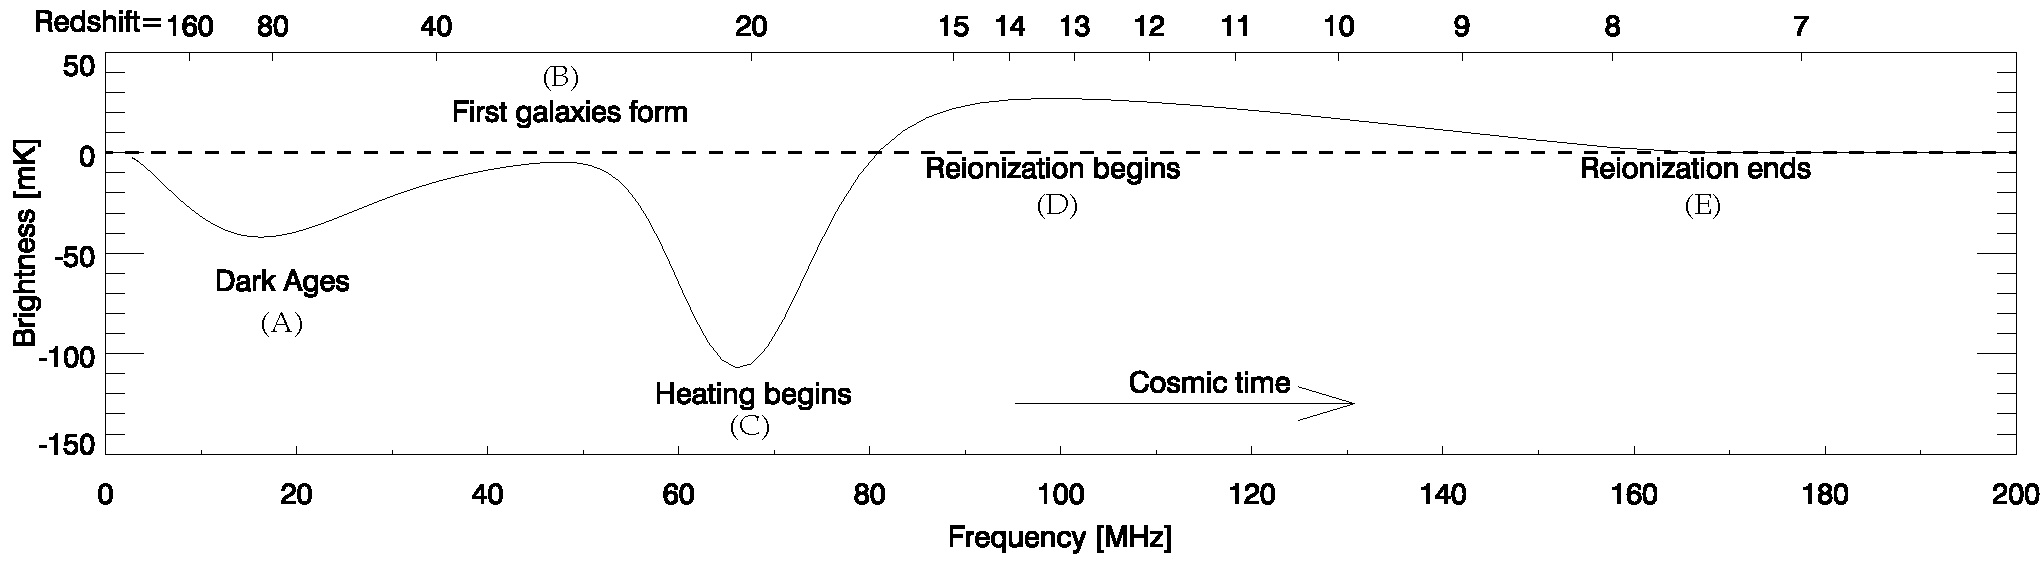
\includegraphics[width=1.\textwidth]{Greig/GlobalSignal}
\includegraphics[trim = 0.2cm 0.6cm 0.2cm 0.2cm, scale = 0.9]{Greig/GSVariation}
\end{center}
\caption{The all-sky averaged (global) 21-cm brightness temperature signal obtained when varying the astrophysical parameters in $\sim~200$ theoretical models. Reproduced from \cite{Cohen:2017}. Copyright of OUP Copyright 2019.}
\label{fig:global_vary}
\end{figure}

\subsection{Power spectrum} \label{sec:PS}

After the global signal, the next simplest and most straightforward approach to characterise the 21-cm signal is through the power spectrum. This is the Fourier transform of the 2-point correlation function. Basically, a measure of the excess signal (above random) on all possible spatial scales. The workhorse statistic for any signal containing structural information, the power spectrum is simply the number of modes (in Fourier space) as a function of physical scale (or size). It produces a distribution of modes characterising the amount of structural information which is contained within the signal. The power spectrum is the natural method for observing the 21-cm signal from a radio interferometer, since these measure differences in the arrival times of the cosmological signal between radio dipoles or dishes of some fixed separation. Thus, a radio interferometer is sensitive to the spatial fluctuations rather than the total amplitude.

To obtain the 21-cm power spectrum, we normalise the 21-cm brightness temperature, $\delta T_{b}(\mathbf{x})$ to be a zero-mean quantity, $\delta_{21}(\mathbf{x}) = (\delta T_{b}(\mathbf{x}) - \delta\bar{T_{b}})/\delta\bar{T_{b}}$, which amplifies the fluctuations (spatial information) in the signal. The power spectrum, $P_{21}(\mathbf{k})$ is computed by the angle-averaged sum of the Fourier transform of the 21-cm brightness temperature fluctuations via,
\begin{eqnarray}
\langle \delta_{21}(\mathbf{k}_{1})\delta^{\ast}_{21}(\mathbf{k}_{2}) \rangle = (2\pi)^{3}\delta_{D}( \mathbf{k}_{1} - \mathbf{k}_{2})P_{21}(\mathbf{k}_{1}),
\end{eqnarray}
where $\delta_{D}$ is the Dirac delta function, $\langle \rangle$ denotes the ensemble average and $^\ast$ corresponds to the complex conjugate. Typically, the 21-cm power spectrum is converted into a dimensionless quantity through $\Delta^{2}_{21}(\mathbf{k}) = (k^{3}/2\pi^{2})P_{21}(\mathbf{k})$. Typically, the Fourier modes are then averaged in spherical shells to obtain the spherically averaged power spectrum, $P_{21}(k)$, which considerably improves the overall signal-to-noise, at the cost of averaging over some spatial information. Alternatively, one can also measure the two-dimensional cylindrically averaged power spectrum, $P_{21}(k_\parallel,~k_\perp)$ decomposing it into modes perpendicular to the line-of-sight ($k_\perp$; spatially averaging the two dimensional angular modes on the sky in annuli) and along the line-of-sight ($k_\parallel$; in frequency) direction. The strength of the two dimensional 21-cm power spectrum is that most of the contamination of the signal by the astrophysical foregrounds can be contained in what is referred to as the EoR `wedge' while the remaining Fourier modes can be clean tracers of the cosmological signal (see Section~\ref{sec:wedge}).

The advantage of the power spectrum over the global signal, is that it provides a measure of the spatial fluctuations in the 21-cm signal. However, it does not encode all the available spatial information from the 21-cm signal. If these fluctuations were truly Gaussian, the power spectrum would contain all the information, and any higher order $n$-point correlation functions would contain no additional information. The structural complexity of the large and small scale processes of reionisation and the cosmic dawn results in the signal being highly non-Gaussian. As such, the power spectrum does not reveal all available information, meaning there is further constraining power from the higher order $n$-point statistics. In section~\ref{sec:bispectrum} and~\ref{sec:trispectrum}  we will return to this. Nevertheless, the power spectrum still contains a wealth of information, and observationally is considerably easier to measure.

\begin{figure}[]
\begin{center}
%\includegraphics[width=1.\textwidth]{Greig/GlobalSignal}
\includegraphics[trim = 0.2cm 0.6cm 0.2cm 0.2cm, scale = 0.4]{Greig/PSMilestones}
\end{center}
\caption{The 21-cm power spectrum amplitude for two different Fourier modes, $k=0.1$~Mpc$^{-1}$ (solid) and $k=0.5$~Mpc$^{-1}$ (dashed). Peaks in the 21-cm power spectrum amplitude correspond to the different cosmic milestones. Reproduced from \cite{Mesinger:2016}. Copyright of OUP Copyright 2019.}
\label{fig:PSMilestones}
\end{figure}

The sensitivity of the 21-cm power spectrum to the underlying astrophysics can be highlighted when we decompose the 21-cm brightness temperature fluctuations through a perturbative analysis (i.e. Taylor expansion) from which we recover the following (see e.g. \cite{Barkana:2005,Santos:2005,Mao:2008}),
\begin{eqnarray}
\delta_{21} \propto C_{b}\delta_{b} + C_{x}\delta_{x} + C_{\alpha}\delta_{\alpha} + C_{T}\delta_{T} - \delta_{\partial v},
\end{eqnarray}
Simply put, fluctuations in the 21-cm brightness temperature field, $\delta_{21}$, are driven by a sum of contributions from the underlying density field, $\delta_{b}$, the ionisation fraction $\delta_{x}$, the Ly$\alpha$ coupling co-efficient, $\delta_{\alpha}$, the temperature of the neutral hydrogen $\delta_{T}$ and line-of-sight peculiar velocity gradient, $\delta_{\partial v}$. Computing the power spectrum then measures the combined signal from the power spectra of each field as well as the cross-power spectra of each. Thus, if we measure the 21-cm power spectrum across cosmic time, we will be sensitive to the epochs when each component dominates (similar to the global signal) and also the spatial scales on which the signal is strongest. This, similar to the global signal, is depicted in Figure~\ref{fig:PSMilestones}.

However, rather than using one single Fourier mode, we have a range of spatial scales over which to recover astrophysical information. This provides access to both the small-scale and large-scale physical processes. For example, during the EoR, the 21-cm power spectrum is dominated by the contribution from the ionisation field, which contains particular structural information on the reionisation process due to the characteristic size of the H$_{\rm \scriptsize II}$ regions as well as their clustering (e.g. \cite{Lidz:2008}). One can equally obtain the spectrum of the sources responsible for heating the IGM from the structural information, owing to the strong dependence of the mean free path with the energy of the X-ray sources. 

\begin{figure}[]
\begin{center}
\includegraphics[trim = 0.2cm 1cm 0.2cm 0.2cm, scale = 0.75]{Greig/ParameterVariation_z9_0_book}
\end{center}
\caption{The three dimensional spherically averaged 21-cm power spectrum at $z=9.0$ when varying astrophysical parameters controlling different astrophysical processes, assuming $T_{\rm S} \gg T_{CMB}$. Top left: the number of ionising photons produced per baryon (ionising efficiency, $\zeta$), top right: maximum ionising photon horizon (proxy for maximum allowable bubble size, $R_{\rm mfp}$) and bottom left: minimum mass of halo hosting star-forming galaxy (represented here as $T_{\rm vir}$). Bottom right: several models at the same ionisation fraction. Reproduced from \cite{Greig:2015}. Copyright of OUP Copyright 2019.}
\label{fig:PSvariation}
\end{figure}

In Figure~\ref{fig:PSvariation} we show the variation in the three dimensional spherically averaged 21-cm power spectrum at a single redshift ($z=9$) when varying three different astrophysical parameters under the assumption of $T_{\rm S} \gg T_{CMB}$~(see e.g. \cite{Greig:2015}). Inset tables correspond to the parameter being varied and the resultant IGM neutral fraction (stage of reionisation). In the top left panel, we vary the ionising efficiency, $\zeta$, a proxy for the number of ionising photons produces by the sources. The shape of the 21-cm power spectrum differs considerably with ionising efficiency. In the early stages, the 21-cm PS matches the density (matter) power spectrum, while in the latter stages it follows the ionisation field. 

Similar behaviour is observed for varying $T_{\rm vir}$, a proxy for the minimum mass of halos hosting star-forming galaxies. Increasing this threshold, results in fewer sources to contribute to reionisation. In the top right panel, the maximum photon horizon, $R_{\rm mfp}$, is varied. Essentially, in this specific work it acts as a maximum allowable bubble size. Note that in this case, the change in $R_{\rm mfp}$ does not alter the neutral fraction strongly, thus the changes in the 21-cm power spectrum are purely as a result in changes to the size of the ionised regions. Finally, in the bottom right we highlight astrophysical models with the same IGM neutral fraction (i.e. the same stage of reionisation). Despite being at the same point in reionisation, the amplitude and shape of the 21-cm power spectrum differs considerably, highlighting the sensitivity of the 21-cm power spectrum to the underlying astrophysical parameters. 

While this example is only for the epoch of reionisation, the same strong sensitivity of the 21-cm power spectrum to the underlying astrophysics is true for both the heating or Ly$\alpha$ coupling epochs. This highlights the strength and utility of the 21-cm power spectrum for recovering the astrophysical information. As such numerous authors have explored the impact of various astrophysical processes on the 21-cm power spectrum (see e.g. \cite{Bowman:2006,Furlanetto:2006a,Iliev:2006,McQuinn:2006,McQuinn:2007,Pritchard:2007,Lidz:2008,Santos:2008,Baek:2010,Harker:2010,Mesinger:2013,Fialkov:2014,Pober:2014,Greig:2015,Geil:2016,Greig:2017b,Hassan:2017,Cohen:2018,Greig:2018,Park:2019,Seiler:2019}).

\subsection{Bispectrum} \label{sec:bispectrum}

The logical extension beyond the power spectrum, the bispectrum, $B$, is simply the Fourier transform of the 3-point correlation function,
\begin{eqnarray}
\langle \delta_{21}(\mathbf{k}_{1})\delta_{21}(\mathbf{k}_{2})\delta_{21}(\mathbf{k}_{3}) \rangle = (2\pi)^{3}\delta_{D}( \mathbf{k}_{1} - \mathbf{k}_{2} - \mathbf{k}_{3})B(\mathbf{k}_{1},\mathbf{k}_{2},\mathbf{k}_{3}),
\end{eqnarray}
where the $\delta_{D}$ enforces that the Fourier modes must form closed triangles. It measures the excess probability of the underlying quantity as a function of three spatial positions in real space. The bispectrum provides a scale-dependent measure of the non-Gaussianity of the 21-cm signal, and as such contains additional astrophysical information beyond that held in the power spectrum. However, it suffers from lower signal-to-noise as there are less modes to average over to boost the signal.

Whereas the power spectrum is relatively trivial to interpret as it is a measure of the power over a single length scale, $k$, the bispectrum is the measure of power over all possible triangle configurations that satisfy the closure condition from $\delta_{D}$. Thus in order to simplify the interpretation of the bispectrum, it is common to consider several simplified triangle configurations. These are typically: (i) the equilateral triangle ($k_{1}  = k_{2} = k_{3}$), (ii) the isosceles triangle ($k_{1} > k_{2} = k_{3}$), (iii) folded triangle ($k_{1} = 2k_{2} = 2k_{3}$), (iv) elongated triangle ($k_{1} = k_{2} + k_{3}$) and (v) the squeezed triangle ($k_{1} \simeq k_{2} \gg k_{3}$). Each, corresponds to different physical properties of the real-space field.

While a detailed discussion of the 21-cm bispectrum is beyond the scope of this chapter, it is fruitful to provide a brief explanation and example of the various configurations (see for example \cite{Lewis:2011} and \cite{Watkinson:2019} for more detailed discussions). The equilateral configuration is essentially an extension of the power spectrum, in the sense that it is expressed as a single amplitude scale, $k$. Generally speaking, it produces the largest amplitude signal and as such is the most commonly studied configuration. It is sensitive to the spherical symmetry of the 21-cm signal such as the scale of the ionised H$_{\rm \scriptstyle II}$ regions during reionisation or the hot/cold spots due to IGM heating. Typically its amplitude grows during the EoR as the signal becomes more non-Gaussian due to the topology of the ionisation field. Shifting towards isosceles or folded triangles, these become more sensitive to planar or filamentary structures in the underlying 21-cm signal. Thus as the topology of either the ionised or X-ray heated regions deviate away from spherical symmetry (i.e. either multiple contributing sources or overlap of ionised regions) the signal should increase with increasing angle. The squeezed limit correlates the small-scale signal from two modes with a large-scale mode, for example capturing the impact of the large-scale environment (i.e. from X-ray heating) on the small-scale power spectrum (i.e. source clustering).

In addition to the structural information in the bispectrum amplitude, the relative sign of the bispectrum under certain triangle configurations and on certain spatial scales can equally reveal insights into the underlying processes. As discussed in \cite{Majumdar:2018,Hutter:2019}, the sign of the bispectrum during reionisation can help distinguish between whether the non-Gaussianity is driven by the topology of the ionised regions (where the bispectrum is negative owing to the below average contribution from the ionised regions) compared to being driven by the matter and cross-bispectra (where it is positive). 

In Figure~\ref{fig:EqBS}, we compare the equilateral bispectrum at $z=7$, 8 and 9 from \cite{Shimabukuro:2017} for differing ionising efficiency, $\zeta$. For decreasing $\zeta$, the amplitude of the bispectrum increases due to its amplitude being dependent on the ionisation fraction. Thus, different reionisation models are easily distinguishable by the 21-cm bispectrum. 

\begin{figure}[]
\begin{center}
\includegraphics[trim = 0.2cm 1cm 0.2cm 0.2cm, scale = 0.5]{Greig/EqBS}
\end{center}
\caption{Variation in the amplitude of the equilateral bispectrum at $z=7$, 8 and 9 for different ionising efficiencies, $\zeta$. Reproduced from \cite{Shimabukuro:2017}. Copyright of OUP Copyright 2019.}
\label{fig:EqBS}
\end{figure}

In recent times, the 21-cm bispectrum has gained considerable traction in interpreting the astrophysics of reionisation and the cosmic dawn (see e.g. \cite{Bharadwaj:2005,Pillepich:2007,Yoshiura:2015,Shimabukuro:2016,Shimabukuro:2017,Watkinson:2017,Majumdar:2018,Hutter:2019,Trott:2019,Watkinson:2019}). Alternatively, rather than exploring the information from the amplitude of the Bispectrum, \cite{Gorce:2019} introduced a three point correlation function based solely on the phases of the Fourier modes (e.g.~\cite{Obreschkow:2013}), termed the triangle correlation function. In focussing solely on the phases, it is sensitive to the characteristic size of the ionised regions and thus exploring the topology of reionisation, which places it in a similar vein as methods to other topological based approaches (Section~\ref{sec:topology}) or the size distribution of ionised regions (Section~\ref{sec:BSDs}). However, not all experiments are designed to measure this phase information. In fact, several experiments are specifically designed to throw away this phase information for increased sensitivity to specific spatial scales. These are referred to redundant configurations and are discussed in Chapter 7.

\subsection{Trispectrum} \label{sec:trispectrum}

Following the Bispectrum, the Trispectrum is the Fourier transform of the four-point correlation function. Already at the level of the Bispectrum, the relative signal-to-noise of the signal is becoming weak, thus, in the foreseeable future it is unlikely a measurement of the Trispectrum during the EoR or earlier will be achievable. Nevertheless, \cite{Cooray:2008} explored the Trispectrum of the 21-cm fluctuations, focussing on fundamental cosmology rather than the astrophysics of the reionisation process. These authors find that the anisotropies from the 21-cm signal are sensitive to primordial non-Gaussianities, an important quantity in constraining inflationary models.

\subsection{One-point statistics}

Rather that measuring the Fourier transform (e.g. power spectrum) of the 21-cm brightness temperature signal, $\delta_{21}(\mathbf{x})$, we can instead measure the one-point statistics (or moments) of the probability distribution function (PDF). In fact, we have already discussed the lowest order one-point statistic, that is, the mean of $\delta T_{b}(\mathbf{x})$ given by the global signal (see \ref{sec:global}).  These one-point statistics of the PDF essentially measure the deviations away from a fully Gaussian PDF, thus they are by definition sensitive to the non-Gaussian nature of the 21-cm signal. Generally speaking, the one-point statistics of $\delta T_{b}(\mathbf{x})$ are given by,
\begin{eqnarray}
m_{n} = \frac{1}{N}\sum^{N}_{i=0}(\delta T_{b}(\mathbf{x_{i}}) - \bar{\delta T_{b}})^{n},
\end{eqnarray}
where $m_{n}$ is the $n$-th order moment and $N$ is the number of pixels over which the signal is measured. For the 21-cm signal, these moments would be generated from the observed two-dimensional tomographic maps of the 21-cm signal.

The next lowest order statistic of the PDF following the mean is the variance, $\sigma^{2}$. The variance is equivalent to the average of the power spectrum over all Fourier modes, $k$,
\begin{eqnarray}
\sigma^{2} = (\bar{\delta T_{b}})^{2} \int \frac{d^{3}k}{(2\pi)^{3}} P(\mathbf{k}).
\end{eqnarray}
As it is the average over all spatial information, the variance itself is less sensitive to the underlying astrophysics than the power spectrum. However, the strength of one-point statistics shines through when using the higher order moments in combination with the variance (or power spectrum). The next two higher order moments are referred to as the skewness and the kurtosis. Equivalent to the variance's relation to the power spectrum, the skewness and kurtosis are the average over all Fourier modes of the bispectrum and trispectrum respectively (the three and four-point correlation functions). As such, whereas the power spectrum only measures the 2-point correlations, the skewness and kurtosis reveals insights from the non-Gaussian properties of the 21-cm signal.

\begin{figure}[]
\begin{center}
\includegraphics[trim = 0.2cm 1cm 0.2cm 0.2cm, scale = 0.45]{Greig/Skewness}
\end{center}
\caption{The variance (left) and normalised skewness (right) of the 21-cm brightness temperature when varying the efficiency of X-ray heating in the IGM. Reproduced from \cite{Watkinson:2015}. Copyright of OUP Copyright 2019.}
\label{fig:skewness}
\end{figure}

The amplitude of the variance is sensitive to differences in the 21-cm brightness temperature. For example, during the EoR, as the number of ionised regions increases (i.e. the contrast between the 21-cm signal from the neutral regions compared to zero signal from the ionised regions) the variance increases. It subsequently turns over as most of the volume is ionised. The skewness is a measure of the asymmetry of the underlying PDF. A negative skewness corresponds to a longer tail towards a lower amplitude signal and a positive skewness corresponds to a longer tail towards higher amplitude signals. The kurtosis is essentially a measure of the outliers of the distribution, with increasing positive (negative) kurtosis corresponding to larger positive (negative) amplitude outliers.

Figure~\ref{fig:skewness} shows an example of both the variance (left) and normalised skewness (right panel) of the 21-cm brightness temperature under different levels of X-ray heating. For increasing X-ray efficiencies (i.e. increase heating) the peak of the variance decreases in amplitude while shifting to earlier times. Increasing the efficiency allows the X-ray heating to occur earlier, reducing the contrast between the $T_{\rm CMB}/T_{\rm S}$ resulting in a lower amplitude peak in the variance. This same behaviour equally results in larger skewness for decreasing X-ray efficiency, owing to a more asymmetric PDF of 21-cm brightness temperatures due to the increasing contrast in $T_{\rm CMB}/T_{\rm S}$. Clearly from Figure~\ref{fig:skewness} it can be seen that these one-point statistics are capable of distinguishing between different astrophysical models. As such, these one-point statistics have been explored in numerous works (e.g. \cite{Wyithe:2007b,Harker:2009,Patil:2014,Watkinson:2014,Watkinson:2015,Kittiwisit:2016,Kubota:2016,Watkinson:2015b,Shimabukuro:2015,Ross:2017}).

Alternatively, the direct 21-cm PDF or the difference PDF have also been studied (e.g. \cite{Barkana:2008,Gluscevic:2010,Ichikawa:2010,Pan:2012}). The difference PDF is the difference between the brightness temperature separated by some spatial scale, $r$. The advantages of the difference PDF is that it can bypass the fact that interferometric observations cannot easily determine the zero flux threshold of the 21-cm signal and that it includes more data by being dependent on spatial scales (similar to two-point correlation functions or the power spectrum). The difference PDF can be more sensitive to the ionising sources and sizes of the ionised regions as it is a direct measure of the distribution of separated pixel pairs that are either both ionised, ionised and neutral or both neutral.

\subsection{Wavelets}

Thus far we have only considered either real-space quantities such as the one-point statistics or the Fourier transform of the $n$-point correlation functions (i.e. the power spectrum and bispectrum). The Fourier transform measures the amplitude of the fluctuations of a given spatial scale, and in order to increase the signal-to-noise we must average the signal over all line-of-sight modes within some observed bandwidth. As a result, we average over modes containing different redshift evolutions and thus increase the bias of the signal. This can be minimised somewhat, for the case of the power spectrum, by averaging the signal over relatively narrow observing bandwidths. However, it still results in some loss in fidelity of the signal.

Instead, in \cite{Trott:2016} the authors explore the potential usage of wavelets, which provide multiple alternatives to the Fourier basis set. Specifically, they explored the application of the Morlet Transform. This provides a family of curves which provide the ability to localise the 21-cm signal both spatially and in frequency. The equivalent to the power spectrum, the Morlet power spectrum is capable of providing an unbiased estimator which maximises the three dimensional nature of the 21-cm signal. Preliminary analysis shows that the Morlet power spectrum performs more optimally than the Fourier power spectrum. A physical interpretation of the Morlet power spectrum in the context of the evolution of the 21-cm signal has yet to be explored.

\subsection{Topological measurements of the 21-cm signal} \label{sec:topology}

Up until this point, we have only discussed methods of characterising the 21-cm signal using just the amplitude of the spatial (e.g. Fourier) information. This is primarily driven by the difficulty in measuring the 21-cm signal and the low signal-to-noise of the first generation experiments. However, the most advanced radio interferometers (such as the Square Kilometre Array, SKA; see Section~\ref{sub_sec:ska}) should be able to provide two dimensional images of the 21-cm signal. That is, they should provide significant signal-to-noise to enable both the amplitude and phase information to be used. 

Direct images of the 21-cm signal contain the complicated morphology of the hot (above average or over dense signal) and cold (below average or under dense signal) of the 21-cm brightness temperature throughout the history of reionisation and the cosmic dawn. The relative sizes, shapes and clustering of these hot/cold patches can reveal numerous insights into the underlying astrophysical processes, such as the number density of sources, their contribution to the heating/ionisation of the IGM and the shape of the emitted spectrum of radiation. The study of these geometric shapes in mathematics is referred to as topology.

Topological studies of reionisation and the cosmic dawn are complimentary to the methods described previously. For example, reionisation proceeds through three main stages (e.g. \cite{Gnedin:2000,Furlanetto:2016}): pre-overlap, over-lap and post-overlap. In pre-overlap, the first ionised H {\scriptsize II} regions (or bubbles) grow completely in isolation roughly until $x_{\rm HI} \geq 0.1$. Over-lap ($ 0.9 \geq x_{\rm HI} \geq 0.1$) describes the merging of these ionised bubbles into essentially a single large connected ionised region. Finally, post-overlap $x_{\rm HI} \geq 0.9$ corresponds to the breaking down of the last remaining patches of neutral IGM into smaller and smaller islands. Topological studies are capable of breaking down these transitions by describing the ratios of ionised and neutral regions, how the ionised (or neutral) regions are connected together and how they are embedded in the larger structures as they form. This provides unique insights into the reionisation epoch not available from statistical methods.

Unfortunately we cannot perform a full pixel by pixel analysis of a measured 21-cm image, therefore we must still compress our images into some form of statistical measurement. There are numerous methods to attempt to characterise the topology of the 21-cm signal. Below, we summarise several of the main approaches taken in the literature. Fundamental to topological studies is the definition of how to identify regions of interest. Typically, a threshold value is required, with the quantity above/below this threshold being used to distinguish the two regions.

\subsubsection{Genus or the Euler characteristic}

The genus, $g$, is a topological property that defines the number of cuts one can make to an object (i.e. H {\scriptsize II} region) without dividing it into independent disconnected sub-regions. It can simply be expressed as,
\begin{eqnarray}
g = N_{\rm >th} - N_{\rm < th}
\end{eqnarray}
where $N_{\rm >th}$ and $N_{\rm < th}$ are the number of connected (or fully enclosed) regions above and below the threshold value for identification. By gradually increasing the threshold value from some initial starting value, a genus curve is constructed, which is a measure of the connectedness of the quantity as a function of different threshold values (e.g. $x_{H {\rm \scriptsize I}}$, $\delta T_{b}$). Typically, these threshold values are expressed in units of the standard deviation from the mean.

The genus has been explored, both in two and three dimensions, either in the context of the ionised (or neutral) field (\cite{Gleser:2006,Lee:2008,Friedrich:2011}) or the 21-cm brightness temperature field (\cite{Hong:2014,Wang:2015}). However, it has yet to be explored in the context of the heating epoch (i.e. $T_{\rm S} \gg T_{\rm CMB}$ is typically assumed). For a purely Gaussian field, the genus curve is symmetric around zero. Thus deviations from symmetry highlight the non-Gaussianity of the 21-cm signal. 

Differences in the evolution in the amplitude of the genus as a function of threshold density can distinguish different source biases and ionising efficiencies. For example, reionisation driven by larger, more biased sources exhibits a different topology than one driven by numerous fainter sources. This appears as changes in the amplitude of the genus as a function of threshold. When the ionised regions are isolated, the genus amplitude is higher than when they begin to overlap (as the total number of isolated ionised regions decreases).

\subsubsection{Minkowski functionals}

A more generalised description of the geometry or topology of the 21-cm signal can be obtained from what are referred to as Minkowski functionals. These are well known concepts from the branch of mathematics known as integral geometry. In $n$-dimensions, there exists $n+1$ independent Minkowski functionals which means that in three dimensional space we have four functionals to describe the topology. Used heavily in cosmology, in particular geometrical features of the galaxy distribution (e.g. \cite{Gott:1986,Schmalzing:1997}) and non-Gaussianity of the CMB (e.g. \cite{Komatsu:2009}), recently they have gained favour for describing the topology of reionisation \cite{Gleser:2006,Friedrich:2011,Yoshiura:2017,Chen:2018}.

For a zero mean scaler function, $u(x)$, (e.g. $\delta T_{\rm b}$) within a volume, $V$, and standard deviation, $u$, we can define an excursion set, $F_{\nu}$, which contains all points that satisfy the threshold, $u(x) \geq \nu\sigma$, where $\nu = u_{\rm th}/\sigma$ and $u_{\rm th}$ is the threshold value. Mathematically, this gives rise to the following Minkowski functionals,
\begin{eqnarray}
V_{0}(\nu) = \frac{1}{V}\int_{V} {\rm d^3}x\,\Theta\left[u(x) - \nu \sigma\right] \\
V_{1}(\nu) = \frac{1}{6V}\int_{\partial F_{\nu}} {\rm d}s \\
V_{2}(\nu) = \frac{1}{6\pi V}\int_{\partial F_{\nu}} {\rm d}s\,\left[\kappa_{1}(x) + \kappa_{2}(x)\right] \\
V_{3}(\nu) = \frac{1}{4\pi V}\int_{\partial F_{\nu}} {\rm d}s\, \kappa_{1}(x)\kappa_{2}(x).
\end{eqnarray}
Here, $\Theta$ is the Heaviside step-function, $\partial F_{\nu}$ is the surface of the excursion set, ${\rm d}s$ is the surface element and $\kappa_{1}(x)$ and  $\kappa_{2}(x)$ are the principle curvatures (inverse of the principle radii) at $x$. The zeroth Minkowski functional, $V_{0}$, corresponds simply to the total volume of the excursion set (i.e. volume above the threshold value), $V_{1}$ and $V_{2}$ correspond to the total surface and mean curvature of the excursion set while $V_{3}$ is the integrated Gaussian curvature over the surface or the Euler characteristic (also $\chi$). The Euler characteristic is related to the genus, $g$, via $V_{3} = 2(1-g)$ thus it effectively describes the shape of the excursion set. Thus, the full set of Minkowski functionals contain additional information beyond that of just the genus.

\begin{figure}[]
\begin{center}
\includegraphics[trim = 0.2cm 1cm 0.2cm 0.2cm, scale = 0.475]{Greig/MFvary}
\end{center}
\caption{The impact of varying the astrophysical parameterisation for a fixed neutral fraction ($x_{H_{\rm \scriptstyle I}}\approx 0.5$) and redshift ($z=8.6$). The coloured curves highlight the impact of varying either the ionising efficiency $\zeta$ or the minimum halo mass for star-forming galaxies, $T_{\rm vir}$ on the four Minkowski functionals. Reproduced from \cite{Yoshiura:2017}. Copyright of OUP Copyright 2019.}
\label{fig:MFs}
\end{figure}

In Figure~\ref{fig:MFs} we show the four Minkowski functionals for the 21-cm brightness temperature when varying the underlying astrophysical processes from \cite{Yoshiura:2017} at a fixed neutral fraction ($x_{H_{\rm \scriptstyle I}}\approx 0.5$) and redshift ($z=8.6$). Here, these authors consider variations in either the ionising efficiency, $\zeta$, or the minimum halo mass hosting star-forming galaxies, $T_{\rm vir}$. Clearly, different reionisation histories are distinguishable by the Minkowski functionals.

Generally speaking the following behaviour is expected of the Minkowski functionals throughout reionisation and the cosmic dawn. $V_{0}$ describes the volume contained above/below the threshold value. For example, if $V_{0} \sim 0.5$ at $\delta T_{\rm b} = 0$ this implies the number of patches above/below the average 21-cm signal are roughly equal. The $V_{0}$ curve will move from left to right (to increasing $\delta T_{\rm b}$) as heating of the IGM occurs. $V_{1}$ (reflected in $V_{2}$) exhibits a similar shift to higher $\delta T_{\rm b}$, however it is initially strongly peaked with a high density tail containing the heated regions. This peak smooths out over a broader range of $\delta T_{\rm b}$ as IGM heating continues. During reionisation, $V_{1}$, $V_{2}$ and $V_{3}$ will shift toward $\delta T_{\rm b}=0$ as the higher amplitude $\delta T_{\rm b}$ regions ionise first.

\subsubsection{Shape-finders}

An extension to Minkowski functionals, shape-finders (\cite{Sahni:1998}) are a way to characterise the shapes of compact surfaces. Applied to reionisation (\cite{Bag:2018,Bag:2019}), these shape-finders can provide a means to characterise how the ionised regions grow. For example, they are useful in being able to distinguish between whether the topology is planar or filamentary. Shape-finders are derived directly from the Minkowski functionals via:
\begin{eqnarray}
{\rm Thickness}: T = \frac{3V_{0}}{V_{1}} \\
{\rm Breadth}: B = \frac{V_{1}}{V_{2}} \\
{\rm Length}: L =  \frac{V_{3}}{4\pi}.
\end{eqnarray}
These shape-finders are interpreted as providing the three principle axes of a physical object. The morphology of the ionised region can then be defined by either the planarity or its filamentarity:
\begin{eqnarray}
{\rm Planarity}: P = \frac{B - T}{B + T} \\
{\rm Filamentarity}: F = \frac{L - B}{L+B},
\end{eqnarray}
where $P\gg F$ corresponds to planar objects (i.e. sheets) while the opposite $F\gg P$ corresponds to a filament.

During the reionisation epoch, percolation theory shows that a single infinitely large, multiply connected ionised region will rapidly form (e.g. \cite{Furlanetto:2016}). When describing the largest singly connected ionised region, \cite{Bag:2018,Bag:2019} find that both $T$ and $B$ evolve slowly whereas $L$ increases rapidly. Thus, this large ionised region grows only along its `length' implying a highly filamentary structure.

\subsubsection{Persistent homology theory}

Homology characterises the topology of the ionisation bubble network into its fundamental components: ionised regions, tunnels (enclosed neutral filaments) and cavities (patches of neutral hydrogen). The persistence then quantifies the significance of the feature, for example its lifetime, by computing a birth and death date for an object.  Thus far, it has only been applied to the ionisation field (\cite{Elbers:2019}). These ionised regions ($\beta_{0}$), tunnels ($\beta_{1}$) and cavities ($\beta_{2}$) can be described by the so-called Betti numbers, $\beta_{n}$, which contain the total number of each type of structure. These can be related to the earlier Euler characteristic via, $\chi = \beta_{0} - \beta_{1} + \beta_{2}$. By breaking the Euler characteristic into the constituent components and tracking their individual growth reveals additional information on the topology, thus it is a more generalised method than either the genus of the Minkowski functionals.

\subsubsection{Fractal dimensions}

An alternative to classifying the ionised (neutral) regions embedded in the 21-cm signal is through a fractal dimensions analysis. Applied to reionisation (\cite{Bandyopadhyay:2017}), this provides a direct means to quantify the deviation away from a homogenous distribution, as well as the degree of clustering and lacunarity (a measure of the size of the ionised regions). The fractal dimension, $D_{q}$, also known as the Minkowski-Bouligand dimension, is a measure of how complicated the topology of the field in question is. A homogeneous distribution in three dimensions has a $D_{q}=3$. \cite{Bandyopadhyay:2017} show that the topology of reionisation exhibits a significant multi-fractal behaviour. These authors find that the fractal dimension is relatively insensitive to the minimum halo mass of the star-forming galaxies, however it was sensitive to the mass averaged ionisation fraction. Thus, the correlation dimension can be useful for constraining the global neutral fraction. Additionally, it is a strong discriminant of models of outside-in and inside-out reionisation.

\subsubsection{Contour Minkowski tensor}

In \cite{Kapahtia:2018,Kapahtia:2019}, these authors introduced the rank-2 contour Minkowski tensor (e.g.~\cite{mcmullen1997,alesker1999,beisbart2002,hug2008,schroder2010,Schroder-Turk:2013}) in two-dimensions which can probe both the length and time scales of the ionised regions during reionisation. The Minkowski tensors are a generalisation of the scalar Minkowski functionals. The contour Minkowski tensor provides information on both the alignment of structures in two dimensions and their anisotropy. Since the ionised regions are not perfectly spherical, their shape anisotropy can be explored by the ratio of the two eigenvalues of the contour Minkowski tensor while the amplitude of the eigenvalues describes their size.

In this analysis, the number of connected regions and holes (e.g. the Betti numbers) given a specific threshold value are tracked. In addition, a characteristic radius of the structures and their shape anisotropy can be determined. For a description of the evolution of $\delta T_{\rm b}$, we refer the reader to \cite{Kapahtia:2019}, ignoring it here owing to its complexity due to the definition of the connected regions and holes as a function of the threshold value as the 21-cm signal transitions transition from above/below average signal regions in the heating epoch to neutral/ionised regions during reionisation. However, we emphasise that these authors explored varying the minimum mass hosting star-forming haloes and clearly show that different astrophysical parameters can be distinguishable.

\subsection{Bubble size distributions} \label{sec:BSDs}

Throughout reionisation and the cosmic dawn, the morphology of the 21-cm signal is driven by processes that embed a morphological signature on the 21-cm signal. For example, the ionised H$_{\rm \scriptsize II}$ regions or the hot (above average signal) or cold (below average signal) spots in the 21-cm brightness temperature during the heating epoch. Quite simply, if we could measure the distribution of these `bubbles' and how they evolve over cosmic time we would have a strong discriminant of the populations of sources responsible for the heating and ionisation of the IGM and also the spectrum of their emitted radiation. Effectively, this would behave as a statistical distribution function (number of bubbles given a physical scale) analogous to a halo mass function. However, the bubbles do not remain isolated, very quickly overlapping into increasingly large and topologically complex structures. Thus, there is no unique way to characterise these bubbles. Nevertheless several methods have been explored in order to be able to construct a probabilistic distribution of the bubble sizes.

The simplest is a friends-of-friends approach (e.g. \cite{Iliev:2006,Friedrich:2011}), which simply connects all cells above (below) a threshold value. However, very rapidly a single large ionised structure exists which fills most of the volume with only a small fraction of isolated regions remaining. The relative volume of this large ionised region and the distribution of the smaller regions can still differentiate reionisation morphologies, however it contains less statistical weight. Alternatively, in \cite{Zahn:2007} a sphere is placed on every pixel, averaging the signal across increasingly larger spheres until a radius is found where the average signal is above the threshold value. While this generates a more statistical meaningful distribution of bubbles, these sizes tend to overestimate the size of the topological feature of interest due to the assumed spherical symmetry.

Recently, more statistically robust methods have been introduced to measure the bubble size distributions. First of these is the mean free path method, which uses a Monte Carlo approach by considering a large number of random positions and determining the distance to the edge of the bubble from different random directions (e.g. \cite{Mesinger:2007}). This results in an unbiased estimator of the bubble size distribution (e.g. \cite{Lin:2016}). 

The Watershed method (e.g. \cite{Lin:2016}) is a more sophisticated approach and has been readily used in the search for cosmological voids. It is a well known two-dimensional image segmentation algorithm creating contours of constant value (i.e. $\delta T_{b}$) which are treated as levels of a tomographic map. These are then `flooded' to obtain unique locations for the minima (e.g. ionised regions). Remaining in the image processing regime, \cite{Giri:2018} introduced the superpixels method. This uses a region based method to identify regions of complex shapes (i.e. ionised regions) segmenting these regions into smaller segments called superpixels. The bubble size distribution is then obtained by averaging the value of the 21-cm brightness temperature within each superpixel before constructing the PDF. Finally, granulometry \cite{Kakiichi:2017} has been investigated, which effectively performs a series of sieving operations to construct a distribution of the sizes of objects which pass through sieves of various sizes and shapes. 

\begin{figure}[]
\begin{center}
\includegraphics[trim = 0.2cm 1cm 0.2cm 0.2cm, scale = 0.45]{Greig/BSDVariation}
\end{center}
\caption{Variation in the bubble size distribution with changes in the underlying astrophysics of the source model. Reproduced from \cite{Geil:2016}. Copyright of OUP Copyright 2019.}
\label{fig:BSD}
\end{figure}

In Figure~\ref{fig:BSD}, we highlight the observed variation in the bubble size distribution at essentially a fixed redshift/neutral fraction from \cite{Geil:2016}. The bubble size distributions here show the characteristic log-normal distribution, with the width of the peak and the relative extents of the asymmetric tails providing sufficient constraining information to distinguish between the various astrophysical models. While several curves appear to produce very similar bubble size distributions, folding in multiple epoch data should be enough to discriminate amongst various astrophysical parameters.

\subsection{Individual images}

Tomographic images of the 21-cm signal provide a direct tangible link to the process of reionisation, revealing the exact locations of ionised regions and potentially even directly observing the sources responsible with targeted follow up observations. For example, individual ionised regions can distinguish between ionisation driven by galaxies and quasars (e.g. \cite{Datta:2012,Majumdar:2012}), and also between other astrophysical sources such as galaxies containing either population II or III stars, mini-quasars, high-mass X-ray binaries or mini-haloes \cite{Ghara:2016,Ghara:2017}. This arises either directly from the size or shape of the ionised region (i.e. larger, more spherical regions in the case of AGN) or from the properties of the 21-cm signal in the immediate vicinity of the ionised region (i.e sharp or gradual changes in the 21-cm signal indicative of the spectrum of emitted ionising or X-ray radiation).

However, the signal-to-noise on a 21-cm image is considerably reduced as we cannot perform an averaging to boost the signal and further we observe the differential brightness temperature which is not necessarily a zero mean quantity, making the definition of an ionised (zero brightness temperature) region complicated. In order to counteract this, matched filters have been one proposed \cite{Datta:2007,Datta:2008,Datta:2012,Majumdar:2012,Malloy:2013,Datta:2016}, which act to minimise the contributions from the noise and foregrounds while maximising the signal by choosing a filter shape consistent with the expected feature of the signal (i.e. spherical ionised region). The 21-cm image is convolved with filters which vary in size and/or shape until the signal-to-noise of the product peaks. A peak in the signal-to-noise corresponds to a feature in the 21-cm image of the same shape as the filter. Matched filters have been explored both in the context of blind and targeted searches of ionised regions.

Alternatively, one can also extract information directly from a 21-cm image using machine learning techniques. Rather than searching for a specific feature (i.e. ionised region), a neural network can be constructed to perform a feature classification to identify regions of interest (see Section~\ref{sec:NN} for more details). Since the 21-cm data is in the form of a 2D (or 3D) image, the preferred network of choice is a convolutional neural network (CNN). The network is constructed using a training set of either 2 or 3D images (i.e. simulated images varying the astrophysical source properties), which undergo a series of down-samplings, convolutions and linear transformations which determine the weights for the various network layers that are used to identify specific features. The network architecture is both user and application specific, and will output user defined properties or parameters. Once the network is constructed, passing an image of the 21-cm signal to the network outputs the desired properties.

In recent years, the usage of CNNs have gained considerable traction. For example, \cite{Hassan:2019a} developed a CNN to distinguish between either AGN or galaxy driven reionisation, \cite{LaPlante:2018} extracted the global history of reionisation from their CNN, and both \cite{Hassan:2019b} and \cite{Gillet:2019} developed CNNs to extract astrophysical or cosmological parameters directly from the input 21-cm image.

\subsection{Stacked images}

Owing to the expected low signal-to-noise measurement for a 21-cm image, and that the individual ionised bubbles may be too small to be directly observed (compared to the resolution of the radio interferometer), \cite{Geil:2017} explored stacking redshifted 21-cm images centred on the known positions of high-redshift galaxies. Such an approach requires a precise determination of the galaxies redshifts on which the stack is centred otherwise the signal will be smeared out.

The resultant stack-averaging of the 21-cm signal produces a notably higher signal-to-noise detection for the mean ionisation profile by averaging out the statistical fluctuations within the IGM. If the IGM is in emission (i.e. heating has occurred), the stack averaged profile is observed in absorption. In contrast, if the IGM is in absorption (i.e. little to no heating) then the stack averaged profile is in emission. This stack-averaged profile then provides a rough estimate of the typical bubble size surrounding galaxies of known absolute UV magnitude which is important for determining if reionisation is driven by many small galaxies or larger, more biased galaxies. However, there remains a degeneracy between the bubble size and the ionisation state of the IGM. A stack of small ionised bubbles can be mimicked by a stack of larger ionised bubbles in a more ionised IGM (owing to the dependence of the mean 21-cm signal on the ionisation state of the IGM).

\subsection{Multi-field approaches}

Thus far we have discussed statistics purely focussed on the 21-cm signal. However, information can also be gleaned from combining the 21-cm signal with other independent tracers of the cosmological information. This can either be performed using a cross-correlation approach, where the 21-cm signal is cross-correlated with an alternative tracer of the galaxy or matter distribution. The advantage of this approach is that the foregrounds between these two fields should be completely uncorrelated, meaning they do not impact the underlying astrophysics of interest. Alternatively, a multi-tracer approach has been proposed, whereby the ratio of two measured fields (one being the 21-cm signal) are taken, which result in the underlying matter perturbations cancelling out leaving behind the interesting astrophysical information.

The leading example of the former approach is the cross-correlation between the 21-cm signal and Ly$\alpha$ emitting galaxies (LAEs; \cite{Wyithe:2007,Wiersma:2013,Sobacchi:2016,Vrbanec:2016,Heneka:2017,Hutter:2017,Hutter:2018a,Kubota:2018}). Here, the idea is that LAEs reside within the ionised regions, where the 21-cm signal is essentially zero (i.e. very little neutral hydrogen). Outside of these regions, the resonant scattering of the Ly$\alpha$ photons by the neutral hydrogen in the IGM strongly attenuates the Ly$\alpha$ line making these LAEs more difficult to detect, however the IGM is visible through the 21-cm signal. Thus, on radii smaller than the typical sizes of ionised regions the signal is anti-correlated. The anti-correlation then decreases to zero, or being slightly positive on much larger radii. The amplitude of this cross-correlation signal, and the rate at which the signal transitions from anti-correlation to zero can be used to determine the neutral fraction of the IGM as well as distinguishing different reionisation morphologies. Alternatives to LAEs have additionally been explored in the literature (\cite{Furlanetto:2007,Lidz:2009,Park:2014,Beardsley:2015}).

In the multi-tracer approach, two or more tracers of the same underlying field (i.e. the large-scale matter density) are used to extract astrophysical information. In taking the ratio of these fields, the matter density field cancels, leaving the astrophysics and cosmological terms. When using the 21-cm signal in combination with a field tracing the high-redshift galaxies, \cite{Fialkov:2019a} found that the anisotropy in the ratio can recover the sky-averaged 21-cm signal, distinguishing various models of the spectral energy distribution of the X-ray sources or the galaxy bias of the high-redshift galaxies. Importantly, in the absence an overlapping high-redshift galaxy survey, any alternative probe of the high-redshift universe can be used including for example planned CO or [CII] line intensity mapping of high-redshift galaxies (e.g. \cite{Kovetz:2017,Moradinezhad:2019a,Moradinezhad:2019b}).

\section{Modelling the 21-cm signal} \label{sec:models}

The 21-cm signal contains a wealth of cosmological and astrophysical information, too complex to be able to interpret without numerical methods. Our ability to learn about the underlying physical processes driving reionisation and the cosmic dawn hinges on being able to perform as physically accurate simulations as possible. However, such simulations require an enormous dynamic range, simultaneously resolving the small-scales (sub-kpc) in order to model the individual sources while also exploring the large-scale ($\sim100$'s of Mpc) radiative transfer effects of the high energy (e.g. X-ray) astrophysical processes responsible for heating and ionising the intergalactic medium. Further, in order to be able to produce an accurate representation of the observed 21-cm signal requires performing multiple simulations to explore the allowed parameter space.

In this section, we explore the various approaches taken within the literature to be able to simulate the 21-cm signal with the ultimate goal of learning as much about the underlying physics as possible. These will include describing the various existing approaches to simulate the 21-cm signal, while others will describe novel methods to inform where in parameter space to concentrate our efforts or methods to bypass performing the simulations all together.

\subsection{Numerical simulations}

Fully numerical simulations are designed to be the most physically accurate approach to investigate the underlying astrophysical processes. These generally consist of simulating the matter (baryons and dark-matter) either through N-body or hydrodynamical methods, and can additionally couple these with radiative transfer (either on-the-fly or post-processing) in order to simulate the radiation transport of the photons responsible for ionising/heating the IGM. The sheer complexity of the dynamic range required to accurately simulate the reionisation process often limits the physical volume of the simulation. However, through advances in computer design and processing power along with the ongoing development of more sophisticated computational algorithms we are continually able to push the boundaries with these types of simulations.

The most physically accurate approach is to perform full radiation hydrodynamical simulations capable of modelling the ionising sources and their interplay with the IGM (e.g. \cite{Ciardi:2001,Gnedin:2006,Finlator:2011,Gnedin:2014,Wise:2014,So:2014,OShea:2015,Norman:2015,Ocvirk:2016,Pawlik:2017,Ocvirk:2018,Rosdahl:2018,Wu:2019}). However, depending on the mass and spatial resolution of the small-scales these are very restrictive in their physical volume ($<100$~Mpc). A computationally cheaper approach is to couple a dark matter only or hydrodynamical simulation with coarser radiative transfer performed in post-processing (e.g. \cite{Iliev:2006,McQuinn:2007,Trac:2007,Ciardi:2012,Iliev:2014,Dixon:2016}). Such an approach enables notably larger simulation volumes to be explored ($<500$ Mpc) better suited for exploring the large-scale astrophysical processes, however, they typically require sub-grid modelling of the astrophysics.

It is through these classes of simulations where we will gain the largest insights into the astrophysical processes driving reionisation and the cosmic dawn. However, the computational cost of running these simulations is too prohibitive to perform a proper parameter exploration of the astrophysical processes. Thus, fully numerical simulations will need to be informed about interesting regions of astrophysical parameter space by analytic or semi-numerical simulations (Section~\ref{sec:efficientsims}).

\subsection{Semi-numerical and analytic models of the 21cm signal} \label{sec:efficientsims}

Rather than attempting to self-consistently model all the astrophysical processes, instead one can judiciously make a number of simplifying approximations in order to drastically increase the computational efficiency of the simulations. This can enable (i) huge cosmological volumes (several Gpc) and (ii) large numbers of simulations to be performed for rapid exploration of the astrophysical parameter space. It's with the approaches discussed below that a lot of progress can be made through being able to perform probabilistic searchers in the full astrophysical parameter space.

Semi-numerical simulations bypass radiative transfer all together, replacing it with an approximate scheme from which the ionisation field can be determined. One of the main approaches to do this is through the excursion-set approach (e.g. \cite{Furlanetto:2004}), which spatially distributes the ionising radiation by comparing the number of ionisations against recombinations in decreasing sized spherical shells (e.g. \cite{Mesinger:2007,Zahn:2007,Geil:2008,Alvarez:2009,Santos:2010,Mesinger:2011,Visbal:2012,Kim:2013,Fialkov:2014,Majumdar:2014,Choudhury:2015,Hassan:2016,Kulkarni:2016,Mutch:2016,Hutter:2018b,Park:2019}). The determination of the number of ionising photons within each grid cell can either be determined from the underlying density field using excursion-set analytic halo mass functions or from identifying the discrete sources directly. Alternatively, one can calibrate a relation between the density field obtained from numerical simulations with properties of reionisation. For example, \cite{Battaglia:2013} use the relation between the redshift of reionisation and the bias of the underlying density field, while \cite{Kim:2016} use a relation between the ionisation fraction and the density.

Instead of bypassing the radiative transfer altogether, one can instead replace the three dimensional radiative transfer with a simple one dimensional radiative transfer and assume spherical symmetry for the distribution of the ionisation fronts (\cite{Thomas:2009,Ghara:2015}) to boost the computational efficiency of the simulations. 

Finally, if we are not interested in the three dimensional structure of reionisation we can construct simplified semi-analytic models which can describe the global history of reionisation and the cosmic dawn. Realistic reionisation histories can be obtained by solving the reionisation equation,
\begin{eqnarray} \label{eq:reion}
\frac{dQ}{dt} = \frac{n_{\rm ion}}{dt} - \frac{Q}{\bar{t}_{\rm rec}}
\end{eqnarray}
where $Q$ is the volume average filling factor of the Universe, $n_{\rm ion}$ is the number of ionising photons produced per baryon and $\bar{t}_{\rm rec}$ is the average recombination time-scale for neutral hydrogen. Using the excursion-set approach applied in one dimension (e.g. \cite{Furlanetto:2004}), we can determine the fraction of collapsed mass above some threshold level (barrier) given some mass threshold (e.g. halo mass). This analytic approach to solve Equation~\ref{eq:reion} has been extensively used in the literature as it gives a rapid and simple estimate of the number of ionising photons required to reionise the Universe \cite{Choudhury:2005,Choudhury:2006,Haardt:2012,Kuhlen:2012,Bouwens:2015,Mitra:2015,Robertson:2015,Khaire:2016,Madau:2017,Mitra:2018,Finkelstein:2019,Mason:2019,Naidu:2019}.

Extending from the excursion-set approach applied in one dimension (e.g. \cite{Furlanetto:2004}), other works have sought semi-analytic approaches to construct statistics describing the reionisation epoch. For example, \cite{Paranjape:2014} developed a model which provides expressions for the bubble-size distribution of the ionised regions, while \cite{McQuinn:2005,McQuinn:2006} explored analytic expressions to describe the 21-cm power spectrum (equivalently, \cite{Barkana:2007} explored the two dimensional correlation function). An alternative semi-analytic approach to describe the global 21-cm signal was developed by \cite{Mirocha:2014,Mirocha:2017,Mirocha:2018}.

\subsection{Intelligent sampling of the parameter space} \label{sec:intel_samp}

Understanding the astrophysics of reionisation and the cosmic dawn will require an exploration of astrophysical parameter space in order to be able to reveal the physical insights describing the observed 21-cm signal. Increasing the complexity, i.e. increasing the number of astrophysical processes or parameters that are simulated can make even these relatively computationally in-expensive semi-numerical simulations inefficient for parameter exploration. However, rather than exploring the entire astrophysical parameter space, we can instead make intelligent choices about which combinations of parameters we choose to sample within our simulations to minimise the computational costs. Such approaches can be useful for obtaining astrophysical parameter constraints directly (when combined with a metric such as a distance relation or likelihood which describes how well the model matches an observation), or for optimal designs for constructing training sets for machine learning approaches (see e.g. Section~\ref{sec:NN}). 

The most na\"{\i}ve approach is to construct a fixed grid of simulations, sampling evenly along each dimension of the astrophysical parameter space. However, as the number of dimensions increases, even this approach can become computationally intractable. An alternative approach is to consider sampling the parameter grid using a Latin-Hypercube approach (\cite{McKay:1979}). Here, the idea is to place points in the parameter grid to ensure no astrophysical parameter is sampled twice (see e.g. \cite{Kern:2017,Schmit:2018}). This approach minimises the overlap amongst the astrophysical parameters in the parameter set. Depending on our purpose, we can improve further on the Latin-Hypercube approach. If we have a reasonable idea with regard to the region of parameter space we expect the signal to occur, we can apply a spherical prior on the parameter space (e.g. \cite{Schneider:2011}). This sphericity drastically reduces the amount of volume in the hyper-surface that needs to be filled with samples (i.e. we ignore the edges of the parameter space). As we increase the dimensionality, the gains in reduction in volume become considerable (see e.g. the discussion in \cite{Kern:2017}).

Alternatively, rather than directly sampling the astrophysical parameter space by drawing from the astrophysical parameters, one can instead adopt a Jeffreys prior (\cite{Jeffreys:1946}). Such an approach searches for regions of the parameter space where the observable (e.g. statistic of the 21-cm signal) varies maximally and increases the sampling within such a region, producing coarser sampling elsewhere. \cite{Eames:2018} explored usage of this Jeffrey's prior in sampling the astrophysical parameter space for reionisation simulations. In addition to the Latin-Hypercube approach described above, they also explored sampling the parameter space using average-eigenvector sampling and adaptive grid-free sampling. The latter two use a hyper-surface distance based metric to inform the placement of points of interest in the parameter space. Such approaches can drastically improve the performance of neural network based approaches by ensuring optimal designs for the training sets (see Section~\ref{sec:NN}).

\subsection{Emulators} \label{sec:emul}

If we are only interested in a statistical description of the 21-cm signal (e.g. 21-cm power spectrum), we can bypass performing the entire numerical or semi-numerical simulations in favour of constructing an emulator. Emulators are a machine learning technique which aims to replicate the desired output of a model using either a series of functional curves (for example polynomials) or a neural network. Once constructed, the emulator provides the desired output statistic describing the signal almost instantaneously given a set of input astrophysical parameters, which can drastically improve parameter exploration. Emulators have been used within astrophysics for a while (see e.g. \cite{Heitmann:2009,Agarwal:2012,Heitmann:2014,Heitmann:2016}), however, only recently have they been explored in the context of reionisation. The construction of an emulator benefits from the intelligent sampling of the astrophysical parameter space (e.g. Section~\ref{sec:intel_samp}) to minimise the size of the required training set.

\cite{Kern:2017} constructed a Gaussian Process (GP) based emulator of the 21-cm power spectrum for the semi-numerical simulation code 21cmFAST \cite{Mesinger:2007,Mesinger:2011}. This emulator takes as input 11 parameters, 5 cosmological and 6 astrophysical, and outputs the 21-cm power spectrum at any redshift during the  reionisation and cosmic dawn epochs. In order to accelerate the training and construction of the emulator, rather than using the raw 21-cm power spectrum outputs ($\Delta^{2}_{21}(k,z)$) a data compression step can be performed to minimise the number of features that the emulator needs to learn. In this work, a principal component analysis (PCA) approach was adopted, which minimises the number of independent pieces of information required to describe the 21-cm power spectrum (i.e. replace the full correlated $k$-bin range, with the sum of a few PCA components). The emulator is then constructed using GP regression to minimise a GP generator function which is completely defined by its mean and covariance within the astrophysical parameter space. For further details, refer to \cite{Kern:2017}.

Alternatively, \cite{Schmit:2018} construct an emulator of the 21-cm power spectrum from 21cmFAST using an artificial neural network (see Section~\ref{sec:NN} for further details and applications). This neural network takes as input the astrophysical parameters describing the model and directly returns an estimate of the 21-cm power spectrum. Evaluating the network to obtain a new 21-cm power spectrum is effectively instantaneous. 

Further, \cite{Jennings:2019} explored several different possible techniques to construct an emulator of semi-numerical simulations. In addition to two simplistic interpolation techniques (i.e. interpolate the result between points in the training set of data), they also explored neural networks, GPs and a support vector machine (SVM). They find that a neural network approach performs best (e.g. \cite{Schmit:2018}) however note that the more sophisticated GP and SVM approaches could be optimised to outperform a neural network emulator.

Instead of simply emulating a function describing the 21-cm signal statistics, recently \cite{Chardin:2019} developed an emulator for the radiative transfer process within reionisation simulations. This approach uses deep learning (another machine learning technique) to output three-dimensional maps of the reionisation time in each cell given an input two dimensional map of the number density of stars and gas. Specifically it uses a trained auto encoder convolutional neural network, which uses layers of two-dimensional convolution kernels to describe the system that is being emulated.

\subsection{Characterising our ignorance}

The trade-off for increased computational efficiency with the semi-analytic and semi-numerical approaches described in Section~\ref{sec:efficientsims} is the reduction in numerical accuracy. When it comes to extracting information about the astrophysics of reionisation and the cosmic dawn from the 21-cm signal, we must therefore be fully aware of the shortcomings of our simulations in order to be able to interpret the results. Further, we must understand in what regimes we can confidently trust these approximate simulations.

For example, in \cite{Santos:2008} some of the analytic models described in Section~\ref{sec:efficientsims} were compared against a hybrid N-body and radiative transfer simulation of cosmic reionisation. Under certain regimes, these analytic models are shown to perform relative well at matching the statistics of the 21-cm power spectrum. Following on from this, \cite{Zahn:2011} explored the comparison between radiative transfer simulations and semi-numerical simulations. In terms of the 21-cm power spectrum, differences between these approaches were found to be of order of 10 per cent in the power spectrum amplitude. With these sorts of comparisons, we can gain confidence that parameter explorations using approximate techniques can reveal useful astrophysical insights. However, for these algorithm comparisons only single astrophysical models were considered. To truly characterise our ignorance a larger, more detailed suite of simulations would be required to fully ascertain how good an approximation they are.

This tens of per cent level uncertainty can be added as an additional modelling uncertainty in attempts to recover astrophysical parameters from the 21-cm signal. This effectively acts as an uncertainty floor, with parameter constraints only available where the impact of the astrophysical parameters on the 21-cm signal is larger than this modelling uncertainty. \cite{Greig:2015,Greig:2019} adopt a 25 per cent modelling uncertainty error to the 21-cm power spectrum finding no biases in the recovery of the astrophysical parameters.

Semi-numerical simulations based on the excursion-set formalism are explicitly photon non-conserving. That is, not all ionising photons are exhausted (i.e. they are lost to the ether) within the simulation. The basis of this, is that the analytic solutions from excursion-set theory are photon conserving in one dimension, however, the three dimensional application in semi-numerical simulations is not. When bubble overlap occurs, ionising photons are not redistributed from the overlap region, they are just unused. This photon non-conservation can result in notably biases in the amplitude of the 21-cm power spectrum \cite{Choudhury:2018} when comparing simulation outputs. However, this photon non-conservation can be trivially accounted for by rescaling the production rates of ionising photons to match the expected global reionisation histories (e.g \cite{Zahn:2011,Majumdar:2014}. Alternatively, more robust corrections can be considered (e.g. \cite{Paranjape:2016,Choudhury:2018,Molaro:2019}).

Provided we are aware of the issues and account for the biases or limitations of the approximate schemes, in most cases we should be able to confidently use these approaches for detailed astrophysical parameter exploration. Of course in practise it is difficult to verify this for each possible astrophysical model or summary statistic.

\section{Inference methods for the 21-cm signal}

In the previous chapters we have discussed the astrophysics and cosmology encoded within the 21-cm signal. In Section~\ref{sec:methods} we discussed numerous ways to characterise the 21-cm signal to tease out the interesting astrophysics, while in Section~\ref{sec:models} we discussed the various approaches to model the 21-cm signal. The final piece to unlocking the astrophysical information from a 21-cm observation is through performing a robust probabilistic exploration of our simulated astrophysical parameter space. This requires comparing the observed 21-cm signal (or a statistic characterising it) against the synthetic output from our simulations, taking into account all forms of possible uncertainties (both observational and theoretical). 

Ultimately, we are interested in obtaining the probability distribution function (PDF) of the entire astrophysical parameter space from our simulated model (or the posterior distribution, $P(\mathbf{\theta}|\mathbf{d})$; the probability of the model astrophysical parameter set, $\mathbf{\theta}$, given the observational data, $\mathbf{d}$). This is what is referred to as the posterior distribution which is obtained from Bayesian statistics through Bayes' theorem,
\begin{eqnarray} \label{eq:Bayes}
P(\mathbf{\theta}|\mathbf{d}) = \frac{P(\mathbf{\mathbf{d}|\theta})P(\mathbf{\theta})}{P(\mathbf{d})},
\end{eqnarray}
where $P(\mathbf{\mathbf{d}|\theta})$ is the likelihood which describes how likely the astrophysical model described by the parameter set $\theta$ describes the data, $P(\mathbf{\theta})$ contains all the prior information we have about the specific astrophysical parameters within our model and $P(\mathbf{d})$ is the evidence which measures how likely the data is given the model. Throughout this section, we will discuss the various approaches considered in the literature for obtaining the posterior PDF. 

\subsection{Fisher Matrices}

One of the simplest and easiest to implement approaches to obtain astrophysical constraints is from the Fisher information matrix (\cite{Fisher:1935}, see e.g. \cite{Tegmark:1997,Coe:2009} for examples how to implement it). This provides a method to quantify the amount of information that an observation contains about any of the unknown parameters in the model parameter set, $\mathbf{\theta}$. The Fisher information matrix, $\mathbf{F}$, is calculated via,
\begin{eqnarray}
\mathbf{F}_{ij} = \left\langle \frac{\partial^{2}{\rm ln}\mathcal{L}}{\partial\theta_{i}\partial\theta_{j}} \right\rangle = \sum_{\mathbf{x}} \frac{1}{\epsilon^{2}(\mathbf{x})} \frac{\partial f(\mathbf{x})}{\partial\theta_{i}} \frac{\partial f(\mathbf{x})}{\partial\theta_{j}} ,
\end{eqnarray}
where $\mathcal{L}$ is the likelihood function (probability distribution of the observed data given the astrophysical parameter set) and $\epsilon$ characterises the error on the measurement of the function, $f(\mathbf{x})$, where $\mathbf{x}$ is the data vector describing the function (i.e. for the 21-cm power spectrum this would be $(k,z)$ the Fourier wavenumber, $k$, and the redshift, $z$). Here, $\mathbf{\theta}$ is the astrophysical parameter set, and we sum the contribution of the partial derivatives of the measured function with each parameter. Parameters which result in large variations in the partial derivatives contain considerable weight and thus highlight which model parameters are sensitive to the function describing the observational data.

Evaluating the Fisher matrix firstly requires the determination of the maximum likelihood model. We can either assume a fiducial parameter set maximises the model, or we can find the model parameter set which is maximal given the observational uncertainties. In the latter case, this can be somewhat computationally expensive, as it requires determining the maximum of our likelihood function.

Once the Fisher information matrix has been calculated, the resultant errors on the model parameters, $\mathbf{\theta}$, given the observation can be obtained by inverting $\mathbf{F}_{ij}$. That is,
\begin{eqnarray}
\mathbf{C}_{ij} = \frac{1}{\mathbf{F}_{ij}},
\end{eqnarray}
where $\mathbf{C}$ is the covariance matrix, with the diagonal entries, $\mathbf{C}_{ii}$, containing the errors on the model parameters (i.e. $\mathbf{C}_{ii} = \sigma^{2}_{ii}$, where $\sigma$ is the standard deviation), and the off-diagonal entries describing the two-dimensional joint probabilities which highlights the degeneracies between those two specific model parameters (i.e. how much similar information each parameter holds).

Fundamentally, the Fisher matrix approach assumes that the observation has been performed optimally, where the uncertainty, $\epsilon$, contains a full description of all sources of error. Further, the inversion of the Fisher matrix to obtain parameter uncertainties assumes that the model parameter set is fully described by a Gaussian likelihood (which is rarely the case in reality). Despite these short-comings, the Fisher matrix provides an excellent and computationally efficient means to provide astrophysical parameter constraints given an observation of the 21-cm signal.

Forecasting of astrophysical or cosmological parameters from during reionisation and the cosmic dawn using Fisher matrices has been extensively used in the literature. For example, with the 21-cm power spectrum \cite{Pober:2014} explored the forecasts for parameters responsible for reionisation, \cite{Liu:2016b} explored similar parameters but coupled with cosmological parameters, while \cite{Ewall-Wice:2016} considered the astrophysical parameters responsible for X-ray heating. Alternatively, \cite{Kubota:2016} explored astrophysics from the variance and skewness of the 1D PDF of 21-cm fluctuations while \cite{Shimabukuro:2017} instead investigated the 21-cm bispectrum and \cite{Pritchard:2010a} explored the global 21-cm signal. Pure cosmology or joint cosmological and astrophysics were additionally investigated using analytic expressions of the reionisation epoch by \cite{McQuinn:2006,Mao:2008,Barger:2009,Visbal:2009,Liu:2016b}.

\subsection{Fixed grid sampling}

The simplest approach to recover the true PDF of our astrophysical parameters (i.e. not under the Gaussian approximation applied in the case of the Fisher matrix) is to construct a grid of astrophysical models which are sampled along the dimensions of the allowed astrophysical parameters. This can either be in a fixed, evenly sampled grid along each dimension or a more informed grid sampling as discussed in Section~\ref{sec:intel_samp} which reduces the number of models required. Once the grid has been constructed, at each grid point we then compare the observed 21-cm signal against the simulated output given that set of astrophysical parameters to assign it a probability (e.g. the likelihood of it being the correct description of the observed data). With this grid of probabilities, we can then interpolate it to generate a full (continuous) description of the underlying PDF (e.g. $P(\mathbf{\theta}|\mathbf{d})$) for this specific astrophysical setup. With this PDF, we can then obtain constraints on any specific astrophysical parameter within our model by marginalising (integrating) over the uncertainties in all other parameters;
\begin{eqnarray}
P(\theta_{1}|\mathbf{d}) = N^{-1} \int P(\mathbf{\theta}|\mathbf{d}) d\theta_{2},d\theta_{3},...,d\theta_{n},
\end{eqnarray}
where $\mathbf{\theta} = (\theta_{1}, \theta_{2}, ..., \theta_{n})$ is the astrophysical parameter set and $N$ is the normalisation constant which ensures $\int P(\mathbf{\theta}|\mathbf{d}) d\mathbf{\theta} = 1$.

Grid based sampling of astrophysical models has been used throughout the literature both for parameter forecasting, as well as inference from observed upper limits on the 21-cm signal. For example, limits on astrophysical parameters during reionisation and the cosmic dawn using the 21-cm global signal have been explored with the Experiment to Detect the Global EoR Signature (EDGES; \cite{Monsalve:2017,Monsalve:2018,Monsalve:2019}) as well as the Long Wavelength Array (LWA; \cite{Fialkov:2019b}). Grids of semi-numerical simulations of reionisation have also been used to interpret existing constraints on reionisation (e.g. such as the optical depth, $\tau_{e}$ \cite{Planck:2018} or limits on the IGM neutral fraction \cite{McGreer:2015}) in the context of PDFs of astrophysical model parameters (e.g. \cite{Mesinger:2012,Mesinger:2013,Greig:2017a}). The equivalent has also been considered for analytic methods \cite{Choudhury:2005,Barkana:2009,Zahn:2012,Mirocha:2018}.

While the fixed grid approach recovers the true underlying PDF and thus is more accurate than the Fisher matrix, it is considerable more computationally expensive due to the increase in number of simulations required. Further, this assumes that the likelihood space is well behaved and varies smoothly. If the likelihood varies sharply, then finer resolution sampling would be required around those regions of parameter space. It is tractable for a low number of astrophysical parameters, but once this goes beyond just a few free parameters it can become infeasible. In the next few sections we discuss techniques to circumvent this.

\subsection{Bayesian MCMC} \label{sec:MCMC}

Once the dimensionality of our astrophysical parameter space becomes too large to directly sample, we must shift to more approximate methods to recover the true PDF of our astrophysical model. In statistics, this is achieved through Markov-Chain Monte-Carlo (MCMC) methods, where we can obtain an estimate of our posterior distribution, $P(\mathbf{\theta}|\mathbf{d})$ through random sampling. To demonstrate the basic idea, we outline one of the simplest MCMC approaches, the Metropolis-Hastings algorithm (\cite{Metropolis:1953,Hastings:1970}). We start with a set of initial positions within our astrophysical parameter space, compute the product of the prior and the likelihood (e.g. the numerator of Equation~\ref{eq:Bayes}) and then take a random jump to a new position in the probability space. In this new position, we compute the product of the prior and likelihood corresponding to the new position, and compare against the previous position. If the new quantity is higher, we keep the new parameter set, if lower, we keep it some fraction of the time according to a probability check (e.g. generate a random number between zero and one and if its higher than the ratio (which is less than one), we keep it). Following this procedure through a large number of iteration, eventually the chain will converge to the peak of the posterior distribution as it must move to regions where the likelihood is higher (i.e. higher probability). To ensure robustness of the sampling (i.e. avoid local minima in our probability space), we perform many Markov-Chains. Once this is complete, simply constructing a histogram of all the sampled points returns an estimate of the posterior distribution (as the most frequent datapoints in the parameter space are those in regions of higher likelihood).

Returning to Bayes' theorem (Equation~\ref{eq:Bayes}), all we require for performing an MCMC is the likelihood ($P(\mathbf{\mathbf{d}|\theta})$) and the prior information ($P(\theta)$). Since at all points within the MCMC we take the ratio of the likelihood multiplied by the prior, we never require the evidence ($P(\mathbf{d})$). This is the advantage of the MCMC approach, as it is the evidence that is the most computationally expensive component of Bayes' theorem (to calculate the evidence we need to perform a multi-dimensional integral over our entire astrophysical parameter space). The last remaining component is the MCMC sampler itself, which is how to determine the new position within the MCMC chain. Within the field of statistics there are many difference types of MCMC samplers all with their own pros and cons, with plenty of literature to assist in deciding which approach is most suitable given the problem.

Over the past decade, the usage of MCMC techniques for the reionisation and the cosmic dawn have been gaining considerable attention. For analytic models that generate reionisation histories that can be coupled with CMB data and other observational constraints, MCMC approaches have been well established (e.g. \cite{Pritchard:2010b,Clesse:2012,Morandi:2012,Mitra:2015,Gorce:2018,Finkelstein:2019,Mason:2019,Naidu:2019}). Analytic models of the global 21-cm signal have also been explored with MCMC, both for interpreting observational limits and also for parameter forecasting for future 21-cm experiments (e.g. \cite{Pritchard:2010a,Harker:2012,Mirocha:2015,Bernardi:2016,Harker:2016}).

Only relatively recently have computational resources become efficient enough to be directly applied to semi-numerical simulations of the 21-cm signal (e.g. \cite{Greig:2015,Greig:2017b,Greig:2018,Greig:2019,Park:2019}). That is, to be able to perform a three dimensional simulation of the 21-cm signal at each set within the MCMC. Alternatively, one can also interpolate over a fixed grid of simulations within an MCMC framework (\cite{Hassan:2017}). Emulators can additionally be coupled to MCMC techniques, whereby the semi-numerical simulation is bypassed with an emulated function describing the 21-cm signal (e.g. \cite{Kern:2017,Schmit:2018}), drastically increasing the computational efficiency. An alternative hybrid approach is to instead train an emulator during the MCMC, to decide whether a new parameter position is close enough to previously sampled positions from which we can emulate the expected result or whether we need to perform the actual likelihood (simulation) call (e.g. \cite{vanderVelden:2019}).

\subsection{Model selection and nested sampling}

Let's return to Bayes' theorem (Equation~\ref{eq:Bayes}), and instead write it explicitly as a function of our chosen astrophysical model, $\mathbf{M}$,
\begin{eqnarray} \label{eq:BayesMS}
P(\mathbf{\theta}|\mathbf{M},\mathbf{d}) = \frac{P(\mathbf{\mathbf{d}|\mathbf{M},\theta})P(\mathbf{\theta}|\mathbf{M})}{P(\mathbf{d}|\mathbf{M})}.
\end{eqnarray}
All terms remain as in Equation~\ref{eq:Bayes}, however, let's focus explicitly on the Bayesian evidence, $P(\mathbf{d}|\mathbf{M})$ (which is often expressed as $\altmathcal{Z}$). This evidence quantifies how likely the observation data was, given our astrophysical model. In traditional MCMC techniques (see previous section), the evidence is ignored as it can be computationally expensive to evaluate and also it is a redundant calculation as we consistently take the ratio of the likelihood to estimate our positions in our astrophysical parameter space. However, if we instead evaluate the evidence term, $\altmathcal{Z}$, we can use this to perform model selection amongst a variety of potentially plausible astrophysical models (i.e. determine which model provides a better representation of the observational data). Herein lies the value of estimating the Bayesian evidence.

Model selection can be performed by taking the ratio of the Bayesian evidence for each model (known as the Bayes factor),
\begin{eqnarray} \label{eq:BayesMS}
\altmathcal{B}_{12} = \frac{P(\mathbf{d}|\mathbf{M}_{1})}{P(\mathbf{d}|\mathbf{M}_{2})}.
\end{eqnarray}
The Bayes factor informs us of the strength of the evidence for one model against another. In other words, if $\altmathcal{B}_{12}$ is greater than unity, then the evidence suggests that model 1 is better than model 2 at modelling our observational data. In \cite{Jeffreys:1961} the Jeffreys scale was introduced to provide a means to classify how strongly the evidence for one model is relative to another. Since then, this scale has been modified several times meaning there is no unique criterion. Here, we adopt the scaling provided by \cite{Lee:2014} which is broken down as follows: (i) if $\altmathcal{B}_{12} > 100$, there is extremely strong evidence for model 1 compared to model 2, (ii) if $30 < \altmathcal{B}_{12} < 100$ there is very strong evidence, (iii) if $10 < \altmathcal{B}_{12} < 30$ there is strong evidence, (iv) if $3 < \altmathcal{B}_{12} < 10$ there is moderate evidence, (v) if $1 < \altmathcal{B}_{12} < 3$ there is anecdotal evidence and (vi) $\altmathcal{B}_{12} = 1$ there is no evidence.

Model selection in the context of reionisation simulations has only relatively recently been explored in \cite{Binnie:2019}. Here, various semi-numerical simulations of reionisation were explored within the context of a mock 21-cm observation. The models differ in how reionisation proceeded (i.e. inside-out compared to outside-in) along with simpler prescriptions for simulating reionisation (i.e. excursion-set compared to a simpler pixel-by-pixel definition \cite{MiraldaEscude:2000}). Using model selection, certain models could be ruled out with mock observations from next generation radio interferometers.

In order to be able to perform model selection, we must be able to compute the Bayesian evidence. This can be achieved using the nested sampling algorithm (e.g. \cite{Skilling:2004}) which performs transformations of the astrophysical parameter space to collapse the multi-dimensional integral for the evidence into a series of more computationally feasible one-dimensional integrals. A convenient byproduct of the nested sampling algorithm is that in order to compute the evidence, one generates samples from the posterior distribution (e.g. $P(\mathbf{\theta}|\mathbf{M},\mathbf{d})$), thus it can perform the same task as a traditional MCMC algorithm. In fact, the particular approach to sampling the astrophysical parameter space within nested sampling can be notably more efficient in regard to the number of required model calls to estimate the posterior distribution. As such, nested sampling is often preferred over traditional MCMC algorithms.

\subsection{Neural Networks} \label{sec:NN}

We have already briefly touched upon neural networks (see Section~\ref{sec:emul}), however, that was in the context of constructing an emulator of the 21-cm power spectrum given input astrophysical parameters. Instead, in this section we flip the problem around and focus on the usage of neural networks to recover estimates of the underlying astrophysical parameters given some input observational dataset. That is, bypass MCMC techniques all together and infer astrophysics directly from a neural network. There have been several works in the literature exploring the validity of using neural networks to perform this task, and we will touch upon the similarities and differences of each of these different approaches.

The fundamental idea of a neural network is to construct a computing system which mimics the behaviour of the brain, containing multiple layers of neurons (see Figure~\ref{fig:ANN} for an example). A neural network must contain an input layer (which processes the input data), any number of hidden layers and a final output layer which produces the desired user defined output (i.e. astrophysical parameters). Each neuron in a layer is connected to all other neurons in adjoining layers (it is not connected within its own layer) and the strength of the connection is driven by what is referred to as the activation function (which takes as input the sum of all results from all other neurons multiplied by the weight of each). We must then train the neural network (the weights returned by each neuron) given the inputs and outcomes of the training set we seek to learn. In order to be able to learn the weights, whats referred to as back propagation is often applied. Here, the aim is to estimate the weights for the network by minimising a cost function. This is an iterative procedure requiring many epochs, and we must be careful not to overfit our network. Thus, the number of epochs is not pre-determined but instead is typically taken to be the value when the cost-function first begins to plateau. We then validate the accuracy of the neural network by comparing the expected outputs from a new dataset (validation dataset, which must differ from the training set) against the returned output from the neural network. Once constructed and validated, the network then almost instantaneously returns the desired user defined outputs given the preferred input format.

\begin{figure}[]
\begin{center}
\includegraphics[trim = 0.2cm 1cm 0.2cm 0.2cm, scale = 1.20]{Greig/ANNexample}
\end{center}
\caption{An example architecture of an artificial neural network. Reproduced from \cite{Shimabukuro:2017b}. Copyright of OUP Copyright 2019.}
\label{fig:ANN}
\end{figure}

\cite{Shimabukuro:2017b} explored the usage of artificial neural networks (ANN) in the context of astrophysical parameter recovery from the 21-cm power spectrum. The network was constructed to take as input a training set of 70 21-cm power spectra varying three astrophysical parameters, and return the expected value given an input 21-cm power spectrum. \cite{Doussot:2019} significantly improved upon this initial ANN approach, considering both a larger training set for the same astrophysical model (2400 models) and supervised learning techniques (techniques to improve the accuracy and optimisation of the constructed neural network, see \cite{Doussot:2019} for more details).

Rather than only using a statistical descriptor of the 21-cm signal (i.e. power spectrum), we could instead use the expected full two or three dimensional 21-cm signal. To do this, we use a convolutional neural network (CNN), whose network architecture is designed to work with images. The main differences between an ANN and CNN is that the CNN requires feature extraction in order to break down the volume of data into a more manageable set. Feature extraction is performed by a series of convolutional and pooling layers on the input image, with each convolutional layer convolving the result with a number of filters to break down the image (see Figure~\ref{fig:CNN} for an example of a CNN) into a simpler set of values to be passed to the neurons of the network. Following feature extraction, the network of neurons is constructed in a similar fashion as in the case of an ANN.

\begin{figure}[]
\begin{center}
\includegraphics[trim = 0.2cm 1cm 0.2cm 0.2cm, scale = 1.05]{Greig/CNNexample}
\end{center}
\caption{An example architecture of a convolutional neural network. Showing the architecture from an input two-dimensional light-cone of the 21-cm signal down to the output astrophysical parameters. Reproduced from \cite{Gillet:2019}. Copyright of OUP Copyright 2019.}
\label{fig:CNN}
\end{figure}

CNNs have been used in a few different ways for reionisation and the cosmic dawn. For example, \cite{Gillet:2019} used two-dimensional light-cones of the simulated 21-cm signal in order to extract the underlying eight astrophysical parameters (from reionisation and X-ray heating) from a mock observation. Similarly, \cite{Hassan:2019b} jointly constrained three cosmological parameters along with three astrophysical parameters from reionisation using two-dimensional images of the 21-cm signal at several redshift snapshots.  Alternatively, \cite{LaPlante:2018} explored recovering the reionisation history from foreground dominated two-dimensional 21-cm images at several redshifts while \cite{Hassan:2019a} used a CNN to perform image classification to determine whether features in the 21-cm image could be distinguished as being driven by galaxies or active galactic nuclei.

Neural networks have been shown to perform extremely well at recovering the expected astrophysics from mock observations, and the evaluation of the neural network for parameter estimation is more computationally efficient than MCMC techniques\footnote{Although the construction of the training set can be as slow or slower than an MCMC, the training set may only need to be constructed once whereas an MCMC must be performed each time.}. However, the fundamental issue with neural networks is their relative inability to provide meaningful uncertainties on the recovered parameters. That is, to characterise how inherent uncertainties in the network construction propagate through into the recovered astrophysical constraints. Contrast this to the recovered posterior distributions from MCMC techniques. Nevertheless, neural networks are an extremely useful and valuable tool for inferring astrophysics about the reionisation and cosmic dawn.

\bibliographystyle{plain}
\bibliography{Greig/References}



\chapter{21~cm observations: calibration, strategies, observables}
\label{chapter:bernardi}

\begin{bf}
  \author{Gianni Bernardi (INAF-IRA \& Rhodes University)}\\
  
Abstract\\

This chapter aims to provide a review of the basics of 21~cm interferometric observations and its methodologies. A summary of the main concepts of radio interferometry and their connection with the 21~cm observables - power spectra and images - is presented. I then provide a review of interferometric calibration and its interplay with foreground separation, including the current open challenges in calibration of 21~cm observations. Finally, a review of 21~cm instrument designs in the light of calibration choices and observing strategies follows.
\end{bf}


%\section{Chapter layout}
%\begin{itemize}
%\item review of basics of interferometry: van-Citter-Zernike theorem, $uv$-coverage, image formation;
%\item from visibilities to power spectra (in particular the delay transform approach - some overlap with Trott's chapter);
%\item interferometric calibration: impact on foreground subtraction, calibration errors redundant calibration;
%\item array design: power spectrum vs imaging, minimmum vs maximum redundancy - some overlap with Trott's chapter?;
%\item impact of calibration errors on power spectra;
%\item ionospheric impact/calibration;
%\item 21-cm image tomography;  
%\end{itemize}

\section{Interferometry overview}

\begin{figure}[]
\begin{center}
\includegraphics[width=1.\textwidth]{Bernardi/2_element_interferometer_1}
%\includegraphics[trim = 0.2cm 0.6cm 0.2cm 0.2cm, scale = 1.0]{Greig/GlobalSignal}
\end{center}
%\caption{A standard schematic of the two element interferometer\footnote{Credit: http://inspirehep.net}.}
\caption{A standard schematic of the two element interferometer (adapted from http://inspirehep.net).}
\label{fig:fig1}
\end{figure}

The Van Cittert-Zernike theorem expresses the fundamental relationship between the sky spatial brightness (or brightness distribution) $I$ and the quantity measured by an interferometer, i.e. the visibility $V$ (e.g., \cite{TMS}):
\begin{equation}
V_{ij} ({\bf b}, \nu) = \int_\Omega {\bar I} (\hat{\bf \sigma}, \nu) \, e^{-2 \pi i \nu \frac{{\bf b} \cdot {\hat {\bf \sigma}}}{c}} d \hat{\bf \sigma},
\label{eq:1}
\end{equation}
where ${\bf b}$ is the baseline vector that separates antenna~$i$ and antenna~$j$, $\nu$ is the observing frequency, $\hat{\sigma}$ is the observing direction (see Figure~\ref{fig:fig1}), $c$ the speed of light and the integral is taken over the source size $\Omega$. 
%The baseline vector is here specified in wavelengths, i.e. ${\bf b} = \frac{{\bf b_{\rm m}}}{\lambda}$, where ${\bf b_{\rm m}}$ is the baseline vector expressed in meters and $\lambda$ is the observing wavelength. 
It can be seen in Figure~\ref{fig:fig1} that the celestial signal travels an extra path between the two antennas, and that length corresponds to a geometrical time delay $\tau = \frac{{\bf b} \cdot {\hat {\bf \sigma}}}{c}$, where the word ``geometrical" refers to the fact that the delay depends upon the source position in the sky and the relative separation between the two antennas. Equation~\ref{eq:1} can be derived as the correlator output. The voltage induced by a celestial source at any antenna can be written in a generic form as $(v \cos{2\pi \nu t})$, and the correlator will output the time average product of the voltages $r$ measured by antenna $i$ and $j$ respectively:
\begin{eqnarray}
r & = & \langle v_i(t)v_j(t) \rangle = \langle v^2 \cos{(2\pi \nu t)} \cos{[2\pi \nu (t - \tau)]} \nonumber \\
			     & = & \langle v^2 \frac{\cos{(2\pi \nu \tau)} + \cos{(4\pi \nu t - 2\pi \nu \tau)}}{2} \rangle. 	
\label{eq:1.1}
\end{eqnarray}
While the first term of the right hand side of equation~\ref{eq:1.1} varies slowly with the Earth rotation, the second oscillates rapidly for any typical radio observations ($\nu > 10$~MHz) and averages to zero, leading to:  
\begin{equation}
r(\tau) = \frac{v^2}{2} \cos{2\pi \nu \tau}.
\label{eq:1.2}
\end{equation}
Equation~\ref{eq:1.2} actually represents the contribution to the fringe from the pointing direction. We can obtained the contribution from the whole source by integrating over the source size and adding the odd (sine) to the even (cosine) fringe component: 
\begin{equation}
R ({\bf b}, \nu) = \int r(\tau) d\tau = \int_\Omega \frac{v^2}{2} \cos{2\pi \nu \tau} - i\sin{2\pi \nu \tau}) = \int_\Omega \frac{v^2}{2} e^{-2 \pi i \nu \frac{{\bf b} \cdot {\hat {\bf \sigma}}}{c}} d \hat{\bf \sigma},
\label{eq:1.3}
\end{equation}
where I have substituted the definition of geometrical delay in the last step. If we note that the $\frac{v^2}{2}$ voltage square term depends upon the direction in the sky as it is proportional to the source brightness, equation~\ref{eq:1.3} is essentially equivalent to equation~\ref{eq:1} and shows how the correlator outputs directly the spatial coherence function of the sky emission, i.e. the visibility.  

The sky brightness distribution does not appear directly in Van Cittert-Zernike theorem, but filtered by the antenna primary beam response $A$ that depends upon the direction in the sky and the wavelength, i.e. ${\bar I} (\hat{\bf \sigma}, \nu) = A (\hat{\bf \sigma}, \nu)  \, I (\hat{\bf \sigma}, \nu)$. The response of the primary beam attenuates the sky emission away from the pointing direction, effectively reducing the field of view $\Omega_F$ of the instrument. Generally speaking, the size of the field of view is essentially given by the antenna diameter $D$: 
\begin{equation}
\Omega_F \approx \frac{\lambda}{D},
\label{eq:2}
\end{equation}
where $\lambda$ is the observing wavelength.

Equation~\ref{eq:1} is often re-written in a different coordinate system, i.e. using the components of the baseline vector $(u,v,w)$, where $(u,v)$ are the components of the baseline vector in the plane of the array and $w$ is the component along the pointing direction $\sigma_0$ (Figure~\ref{fig:fig1b}). The sky position in the $\hat {\sigma}$ direction can be decomposed into the $(l,m)$ components parallel to the plane of the sky and the $n$ along the $w$ axis. In this system, coordinates can be re-written as (\cite{TMS}):
\begin{eqnarray}
\frac{\nu \, {\bf b} \cdot {\hat {\bf \sigma}}}{c} & = & ul + vm + wn, \nonumber \\
\frac{\nu \, {\bf b} \cdot {\hat {\bf \sigma}}_0}{c} & = & w, \nonumber \\
d\Omega & = & \frac{dl dm}{n} = \frac{dl dm}{\sqrt{1 - l^2 - m^2}}
\label{eq:2.1}
\end{eqnarray}
and equation~\ref{eq:1} then becomes:
\begin{equation}
V_{ij} (u,v,w, \nu) = \int_\Omega {\bar I} (l, m, \nu) \, e^{-2 \pi i (ul + vm + w(\sqrt{1 - l^2 - m^2} - 1))} \frac {dl \, dm \, dn}{\sqrt{1 - l^2 - m^2}}.
\label{eq:3}
\end{equation}
%
\begin{figure}[]
\begin{center}
\includegraphics[width=1.\textwidth]{Bernardi/coordinates_imaging}
\end{center}
\caption{Cartoon representation of the coordinate system used for interferometric imaging. The $(l,m)$ plane is tangent to the sky.}
\label{fig:fig1b}
\end{figure}
%
Although low frequency radio observations are intrinsically wide-field, for the purpose of studying the 21~cm observables, we can reduce equation~\ref{eq:3} to a two dimensional Fourier transform:
\begin{equation}
V_{ij} (u,v, \nu) = \int_\Omega {\bar I} (l, m, \nu) \, e^{-2 \pi i (ul + vm)} dl \, dm.
\label{eq:4}
\end{equation}
Equation~\ref{eq:4} indicates that an {\it interferometer measures the two dimensional Fourier transform of the spatial sky brightness distribution}. If our goal is to reconstruct the sky brightness distribution, equation~\ref{eq:4} can be inverted into its corresponding Fourier pair:
\begin{equation}
%{\bar I} (l, m, \lambda) = \int_{- \infty}^{+ \infty} V_{ij} (u,v, \lambda) \, e^{2 \pi i (ul + vm)} du \, dv.
{\bar I} (l, m, \nu) = \int V_{ij} (u,v, \nu) \, e^{2 \pi i (ul + vm)} du \, dv.
\label{eq:5}
\end{equation}
Equation~\ref{eq:5} is, however, a poor reconstruction of the sky brightness distribution as only one Fourier mode is sampled at a single time instance. Strictly speaking, indeed, all the quantities in equation~\ref{eq:4} and \ref{eq:5} are time variable. In most cases, the time dependence of the primary beam and the sky brightness distribution can be neglected, however, this is not the case for the visibility $V$ as the projection of the baseline vector with respect to the source direction changes significantly throughout a long (e.g. a few hours) track. In this way, many measurements of the visibility coherence function $V$ can be made as $(u,v)$ change with time, allowing for a better reconstruction of the ${\bar I} (l, m, \nu)$ function. This method is commonly referred to as {\it filling the $uv$ plane via Earth rotation synthesis} and was invented by \cite{ryle60}. The other (complementary) way to fill the $uv$ plane is to deploy more antennas on the ground in order to increase the number of instantaneous measurements of independent Fourier modes. If $N$ antennas are connected in an interferometric array, $\frac{N (N - 1)}{2}$ instantaneous measurements are made. 

The combination of a large number of antennas and the Earth rotation synthesis, defines the sampling function $S(u,v)$ in the $uv$ plane. In any real case, equation~\ref{eq:5} can therefore be re-written as:
\begin{equation}
{\bar I}_D (l, m, \nu) = \int S(u,v, \nu) V (u,v, \nu) \, e^{2 \pi i (ul + vm)} du \, dv,
\label{eq:6}
\end{equation}
where ${\bar I}_D$ indicates the sky brightness distribution sampled at a finite number of $(u,v)$ points (often termed {\it dirty image}) and where the explicit dependence on the antenna pair was dropped for simplicity. Using the convolution theorem, equation~\ref{eq:6} can be re-written as:
\begin{equation}
{\bar I}_D (l, m, \nu)  =  \tilde{S \, V} =  {\tilde S} \ast {\tilde V} = {\rm PSF} (l, m, \nu) \ast {\bar I} (l, m, \nu),
\label{eq:7}
\end{equation}
where the tilde indicates the Fourier transform, $\ast$ the convolution operation and PSF is the Point Spread Function, i.e. the response of the interferometric array to a point sources which, in our case, is also the Fourier transform of the $uv$ coverage.

%I will give some examples of sampling functions for different instruments in Section~\ref{sec:design}, however, 
The sampling function always effectively reduces the integral over a finite (often not contiguous) area of the $uv$ plane. In particular, the sampled $uv$ plane is restricted to a minimum $uv$ distance that cannot be shorter than the antenna\footnote{In this chapter I use the words ``antenna" and ``station" interchangeably to indicate the correlated elements even if, in the literature, they are normally used to indicate a dish and a dipole, or a cluster of dipoles, respectively.} size and the largest separation between antennas, i.e. the maximum baseline ${\bf b}_{\rm max}$. The maximum baseline also sets the maximum angular resolution $\theta_b$:
\begin{equation}
\theta_b \approx \frac{\lambda}{|{\bf b}_{\rm max}|}.
\label{eq:8}
\end{equation}
The incomplete sampling of the $uv$ space leads to a PSF that has ``sidelobes", i.e. nulls and secondary lobes that can often contaminate fainter true sky emission. The best reconstruction of the sky brightness distribution ${\bar I}$ requires deconvolution of the dirty image from the PSF. 

Figure~\ref{fig:fig1c} and \ref{fig:fig1d} provide an example of the sampling $S(u,v,)$ and corresponding point spread function. A single baseline essentially imprints a (sinusoidal) fringe pattern on the sky, whose period and phase depend upon the baseline length and orientation respectively (equation~\ref{eq:1}). The combination of more baselines of different lengths and orientations improves the sampling function until a good quality point spread function is obtained.
%
\begin{figure}[]
\begin{center}
\includegraphics[width=1.\textwidth]{Bernardi/fringe_bl_11_18}
\includegraphics[width=1.\textwidth]{Bernardi/fringe_bl_17_15}
\end{center}
\caption{Left panel: one baseline selected (indicated with a red line) from 32 antennas distributed within a 350~m circle (taken from \cite{jacobs11}). Right panel: corresponding point spread function. For a single baseline case the point spread function is essentially a sinusoidal fringe pattern whose period is inversely proportional to the baseline length, i.e. the pattern correponding to $\sim 50$~m baseline (top) oscillates approximately seven times slower than a $\sim 350$~m baseline (bottom). The fringe phase (i.e. the pattern orientation) is given by the baseline orientation.}
\label{fig:fig1c}
\end{figure}
%
\begin{figure}[]
\begin{center}
\includegraphics[width=1.\textwidth]{Bernardi/fringe_5bls}
\includegraphics[width=1.\textwidth]{Bernardi/fringe_all}
\end{center}
\caption{Same as Figure~\ref{fig:fig1c}, but including five baselines with different lengths and orientations (red lines, top panel) and all the baselines (for $N = 32$ there are 496 baselines; bottom panel) simultaneously. The fringe pattern is already noticeably different when five baselines are included with respect to the single baseline, although a clean point spread function only appears when all the baselines are used simultaneously (bottom panel).}
\label{fig:fig1d}
\end{figure}





\section{21~cm observables: power spectra and images}
\label{sec:observables}

The ultimate goal of 21~cm observations is to image the spatial distribution of the 21~cm signal as a function of redshift, also known as {\it 21~cm tomography}. Given the curent theoretical predictions, such observations need to achieve mK sensitivity on a few arcminute angular scales (see Chapter~1 in this book). Most of the current arrays, however, only have the sensitivity to perform a statistical detection of the 21~cm signal, i.e. to measure its power spectrum. Given an intensity field $T$, function of the three dimensional spatial coordinate $\bf x$, its power spectrum $P(k)$ is defined as:
\begin{equation}
%\langle {\tilde T}^* ({\bf k}) {\tilde T}({\bf k'}) \rangle = (2 \pi)^3 P({\bf k}) \delta^3({\bf k} - {\bf k}')
\langle {\tilde T}^* ({\bf k}) {\tilde T}({\bf k'}) \rangle = (2 \pi)^3 P(k) \delta^3({\bf k} - {\bf k}')
\label{sec_observables_eq1}
\end{equation}
where $\langle \rangle$ indicates the ensamble average, $\bf k$ is the Fourier conjugate of $\bf x$, tilde the Fourier transform, $^*$ the conjugate operator, $k$ the magnitude of the $\bf k$ vector and $\delta$ the Dirac delta function. In 21~cm observations, power spectra can be computed from interferometric image cubes after deconvolution of the dirty image ${\bar I}_D (l,m,\nu)$ from the point spread function (e.g., \cite{pen09}, \cite{harker10}, \cite{beardsley16}, \cite{patil17}). Alternatively, the 21~cm power spectrum can be estimated directly from the interferometric visibilities. Equation~\ref{eq:4} already shows that the interferometer is a ``natural" spatial power spectrum instrument (e.g., \cite{white99} and Figure~\ref{fig:fig1c}, \ref{fig:fig1d}). Visibilities can be further Fourier transformed along the frequency axis (the so-called {\it delay transform}, \cite{parsons12a}): 
\begin{equation}
{\tilde V}_{ij} (u,v, \tau) = \int_B V (u,v, \nu) \, e^{-2 \pi i \nu \tau} d \nu
\label{sec_observables_eq2}
\end{equation}
where $B$ is the observing bandwidth and $\tau$ is the geometrical delay. The delay transform is therefore proportional to the three dimensional power spectrum (\cite{parsons12b}):
\begin{equation}
P(k) \propto {\tilde V}_{ij} (|{\bf b}|, \tau),
\label{sec_observables_eq3}
\end{equation}
where the proportionality constant transforms the visibility units into power units (\cite{parsons12b}). The observer units $({\bf b},\tau)$ map directly in $k$ modes parallel and perpendicular to the line of sight (e.g., \cite{morales04}):
\begin{equation}
k_\perp = \frac{2 \pi |{\bf b}|}{D_c} = \frac{2 \pi \sqrt{u^2 + v^2}}{D_c}, \,\,\,\,\,\,\,    k_\parallel = \frac{2 \pi f_{21} H_0 E(z)}{c \, (1 + z)^2} \, \tau,
\label{sec_observables_eq4}
\end{equation}
where $D_c$ is the transverse comoving distance, $f_{21} = 1421$~MHz, $H_0$ is the Hubble constant and $E(z) = \sqrt{\Omega)m (1+z)^3 + \Omega_k (1+z)^2 + \Omega_\Lambda}$. Due to the dependence of the geometrical delay upon frequency, equation~\ref{sec_observables_eq3} is only valid for short baselines, typically shorter than a few hundresd meters, for which the geometrical delay is fairly constant across the bandwidth and lines of constant $k_\parallel$ are essentially orthogonal to the $k_\perp$ axis (\cite{parsons12b}).

Equation~\ref{sec_observables_eq2} does not only provide a link between visibilities and three dimensional power spectra, but also introduces the concept of ``horizon limit", i.e. the maximum physical delay allowed $\tau_{\rm max} = \frac{|{\bf b}|}{c}$, where $c$ is the speed of light. The most relevant implication of the existence of a horizon limit is the definition of a region in the two dimensional $(k_\parallel,k_\perp)$ power spectrum space where smooth-spectrum foregrounds are confined, leaving the remaining area  uncontaminated in order to measure the 21~cm signal (the so-called ``Epoch of Reionization (EoR) window", Figure~\ref{fig:fig2}). Foregrounds can therefore be ``avoided" with no requirements for subtraction (e.g., \cite{morales12}, \cite{vedantham12}, \cite{pober13}, \cite{thyagarajan13}; see also Chapter~6 in this book).
\begin{figure}[]
\begin{center}
\includegraphics[width=1.\textwidth]{Bernardi/delay_transform}
\end{center}
\caption{Amplitude of delay transformed visibilities as a function of time and delay for a 32 (top let), 64 (top right), 128 (bottom left) and 256~m (bottom right) baselines respectively (from \cite{parsons12a}). A number of smooth spectrum point sources are simulated as foregrounds and their tracks are clearly bound within the horizon limit (black dashed line). The cyan emission is a fiducial 21~cm model that has power up to high delays regardless of the baseline length.}
\label{fig:fig2}
\end{figure}
The choice of a foreground avoidance strategy versus subtraction plays an important role in planning an experiment, its related observing strategy and the array calibration strategy.

The requirements for image tomography are the same as for high brightness sensitivity observations of diffuse emission like the Cosmic Microwave Background (e.g., \cite{halverson02}, \cite{dickinson04}, \cite{readhead04}). The 21~cm spatial distribution throughout cosmic reionization has structures on 5-10 arcminutes up to degree scales (e.g., \cite{majumdar12}, \cite{datta12}, \cite{mellema13}, \cite{kakiichi17}). In order to image 21~cm fluctuations, a maximum baseline of the order of a few km gives a resolution of a few arcminutes in the $100-200$~MHz range, together with filled $uv$ plane in order to accurately reconstruct their complex spatial structure. A filled $uv$ plane also leads to a point spread function with very low sidelobes, making the deconvolution process easier (see the bottom right panel of Figure~\ref{fig:fig1d} for an example of densely sampled $uv$ plane that leads to a good quality point spread function). The most stringent requirements for image tomography remain the accurate foreground separation and, as I will review in the next section, the related instrumental calibration.



%\section{Challenges in 21~cm observations: interferometric calibration in presence of bright foreground emission, wide fields of view, ionosphere}
\section{Interferometric calibration and 21~cm observations}
\label{sec:challenges}

Celestial radio signals always experience a corruption when observed with an interferometric array, due to the non-ideal instrumental response that is corrected in post processing in a process that is known as interferometric calibration. Calibration relies on the definition of a data model where the corruptions are described by antenna based quantities known as Jones matrices. Such data model is known as the interferometric measurement equation (\cite{hamaker96},\cite{smirnov11},\cite{smirnov11b},\cite{smirnov11c}).

If antenna $1$ and antenna $2$ measure two orthogonal, linear polarizations $x$ and $y$, the cross-polarization visibility products can be grouped in a $2 \times 2$ complex matrix ${\bf V}$:
\begin{equation}
    {\bf V}_{12} (u,v,\nu) \equiv 
    \left[ 
    \begin{array}{cc}
    V_{12,xx} (u,v,\nu) & V_{12,xy} (u,v,\nu) \\
    V_{12,yx} (u,v,\nu) & V_{12,yy} (u,v,\nu) \\
    \end{array}
    \right].   
\label{eq:sec:1}
\end{equation} 
The sky brightness distribution $I$ can also be written as a $2 \times 2$ matrix ${\bf B}$ using the Stokes parameters as a polarization basis:
\begin{equation}
    {\bf B}_I (l,m,\nu) \equiv 
    \left[
    \begin{array}{cc}
    I (l,m,\nu) + Q (l,m,\nu) & U (l,m,\nu) + iV (l,m,\nu) \\
    U (l,m,\nu) - iV (l,m,\nu) & I (l,m,\nu) - Q (l,m,\nu) \\
    \end{array}
    \right].   
\label{eq:sec:2}
\end{equation} 
At this point, equation~\ref{eq:3} can be written by including the corruptions represented by the complex Jones matrices $J$: (\cite{hamaker96},\cite{smirnov11}):
\begin{equation}
{\bf V}_{12} (u,v,\nu) = {\bf J}_1 \left( \int_\Omega {\bf B}_I (l, m, \nu) \, e^{-2 \pi i (ul + vm)} dl \, dm  \right) {\bf J}_2^H,
\label{eq:sec:3}
\end{equation}
where $H$ is the Hermitian operator.
 
Equation~\ref{eq:sec:3} is known as the {\it measurement equation} and is the core of interferometric calibration. For an array with $N$ antennas, equation~\ref{eq:sec:3} can be written for each of the $\frac{N (N - 1)}{2}$ visibilities forming an overdetermined system of equations. The development of  algorithms to solve the calibration system of equations is a very active research line (\cite{mitchell08}, \cite{kazemi11}, \cite{tasse14}, \cite{yatawatta15}, \cite{smirnov15}) although beyond the scope of this chapter and we mention it here for completeness.

The solution of the measurement equation requires some knowledge of the sky brightness distribution ${\bf B}_I$, in other words, a {\it sky model}. Traditionally this is achieved by observing a calibration source, i.e. a bright, unresolved point source with known spectral and polarization properties. Calibration solutions are then applied to the observed field that is then used to improve the sky model ${\bf B}_I$ which, in turn, leads to more accurate calibration solutions ${\bf J}$. This loop is traditionally called self calibration (\cite{cornwell81}, \cite{pearson84}) and can lead to a highly accurate calibration (e.g., \cite{bernardi10}, \cite{smirnov11b}).

The advantage of the measurement equation is that it can factorize different physical terms into different matrices. For example, the frequency response of the telescope electronics and its time variations essentially affects only the two polarization responses and are modeled with a diagonal Jones matrix ${\bf B}$:
\begin{equation}
    {\bf B} (t,\nu) \equiv 
    \left[
    \begin{array}{cc}
    b_x (t,\nu) 	& 	0 	\\
    0 		& b_y (t,\nu) 	\\
    \end{array}
    \right],   
\label{eq:sec:4}
\end{equation} 
where we made it explicit that ${\bf B}$ can vary with time and frequency. The undesired instrumental leakage between the two orthogonal polarized can be written as a ${\bf D}$ Jones matrix of the form:
\begin{equation}
    {\bf D} (t,\nu) \equiv 
    \left[
    \begin{array}{cc}
    1	 		& d_x (t,\nu)	\\
    -d_y (t,\nu)	& 1 	\\
    \end{array}
    \right],   
\label{eq:sec:5}
\end{equation} 
and the measurement equation can be written as:
\begin{equation}
{\bf V}_{12} (u,v,\nu) = {\bf B}_1 \, {\bf D}_1 \left( \int_\Omega {\bf B}_I (l, m, \nu) \, e^{-2 \pi i (ul + vm)} dl \, dm  \right) {\bf D}_2^H  \, {\bf B}_2^H.
\label{eq:sec:6}
\end{equation}
We note that, in principle, the primary beam response should appear as an additional $2 \times 2$ Jones matrix before the ${\bf D}$ matrix. For the purpose of this section we will neglect it, although we will illustrate an exception to this assumption when we later discuss polarization calibration.

Retaining only the first order terms, equation~\ref{eq:sec:6} can be written as (\cite{sault96}):
\begin{eqnarray}
V_{12,xx} (u,v,\nu) & = & b_{1,x} \, b_{2,x}^* [V_I (u,v,\nu) - V_Q (u,v,\nu)]\\
V_{12,xy} (u,v,\nu) & = & b_{1,x} \, b_{2,y}^* [(d_{1,x} - d_{2,y}^*) V_I (u,v,\nu) + V_U (u,v,\nu) + iV_V (u,v,\nu)]	\\
V_{12,yx} (u,v,\nu) & = & b_{1,y} \, b_{2,x}^* [(d_{2,x} - d_{1,y}^*) V_I (u,v,\nu) + V_U (u,v,\nu) - iV_V (u,v,\nu)]	\\
V_{12,yy} (u,v,\nu) & = & b_{1,y} \, b_{2,y}^* [V_I (u,v,\nu) - V_Q (u,v,\nu)],
\label{eq:sec:7}
\end{eqnarray}
where I dropped the explicit dependence on time and wavelength from the gain terms for notation clarity, and where $V_{i=I, Q, U, V}$ are the Fourier transforms of the elements of the sky brightness matrix ${\bf B}$.

This form of the measurement equation offers an intuitive understanding as to why calibration is of paramount importance in 21~cm observations. The observed visibilities are essentially a measurement of foreground emission and, in the ideal case, their amplitudes would vary smoothly with frequency, allowing to avoid or subtract foregrounds. However, the instrumental response inevitably corrupts this smoothness in several ways: because the telescope primary beam is not sufficiently smooth in frequency, because of the electronic response or because of reflections along the signal path. Although calibration will correct for these effects and restore the intrinsic foreground frequency smoothness, calibration errors (i.e., deviations from the true ${\bf B}$ solutions) will still corrupt the foreground spectra. In practice, calibration errors result in foreground power leaking out of the horizon limit and jeopardizing (part of) the EoR window. The corruption of the foreground spectra will limit the accuracy of any subtraction method (see discussion in Chapter~6 in this book). {\it The effectiveness of foreground separation, proven in ideal cases, depends significantly on the accuracy of interferometric calibration.}

The form of the measurement equation written in equations~\ref{eq:sec:6} and \ref{eq:sec:7} is often referred to as a {\it direction independent} calibration as it implicitly assumes that a single Jones matrix is sufficient to describe corruptions across the whole sky area of interest. This assumption is often invalid at low frequencies, mostly because of the changing primary beam response over a wide field of view, frequency, and the course of the observation, and the position and time dependent corruptions introduced by the Earth's ionosphere. In this case the measurement equation becomes {\it direction dependent}, i.e. a different Jones matrix is written and solved for a certain number of directions in the sky:
\begin{equation}
{\bf V}_{12} (u,v,\nu) = \sum_s \left[ {\bf B}_{1,s} \left( \int_\Omega {\bf B}_{I,s} (l, m, \nu) \, e^{-2 \pi i (ul + vm)} dl \, dm  \right) {\bf B}_{2,s}^H \right],
\label{eq:sec:7_added}
\end{equation}
where the sum is over the number of directions $s$. We note that we have used the ${\bf B}$ matrix for pedagogical purposes here, regardless of the physical origin of the direction dependent effect. Direction dependent effects also impact foreground separation, in a similar way as the direction independent effects.
 
Accurate direction independent and dependent calibration of 21~cm observations is a key topic of present research and can be grouped in a few main topics: 
%
\begin{itemize}
\item {\it sky models}. Ideally, the sky brightness model matrix ${\bf B}_I$ (equation~\ref{eq:sec:6} and \ref{eq:sec:7}) would include the whole sky emission. This is pratically impossible as part of the sky signal is the unknown of interest (the 21~cm signal) and the detailed properties of the foreground sky are not known sufficiently well. \begin{figure}[]
\begin{center}
\includegraphics[width=1.\textwidth]{Bernardi/calibration_errors}
\end{center}
\caption{Example of power spectrum bias introduced by calibration errors due to an incomplete sky model for the Murchison Widefield Array (MWA, left) and the Low Frequency Array (LOFAR, right) cases respectively (adapted from \cite{ewall-wice17}). Power spectra are shown in their two dimensional $(k_\perp,k_\parallel)$ form in order to display the foreground dominated region below the horizon limit (grey solid line). Cyan, orange and red lines are the locii where a fiducial 21~cm model power spectrum is one, five and ten times higher than the bias level. In an ideal case with perfectly smooth foregrounds and no calibration errors, the 21~cm power spectrum should be detectable just outside the horizon limit. The errors introduced by an incomplete sky model leak foreground power in the EoR window at a level that may completely prevent a detection in the MWA case.}
\label{fig:fig_added}
\end{figure}
Sky models are normally constituted of a catalogue of compact sources of known (or measured) properties, often covering an area significantly larger than the telescope field of view (e.g., \cite{yatawatta13}, \cite{pober16}). Nevertheless, sky models remain essentially always incomplete at some level, as source catalogues are limited in depth, source characterization and - often - sky coverage. \cite{grobler14}, \cite{wijnholds16} and \cite{grobler16} show that incomplete catalogues used as sky models bias the calibration and eventually lead to artifacts in the form of ghost-like sources in interferometric images, most of the times fainter than the image noise level. The ghost pattern is stronger for regularly spaced arrays and if the sky model is less complete. In terms of power spectrum, \cite{ewall-wice17} and \cite{barry16} show that the calibration bias introduced by incomplete sky models leads to an overall leakage of foreground power in the EoR window (Figure~\ref{fig:fig_added}). A similar foreground leakage may occur because of the finite angular resolution of interferometric observations: for example, two sources whose size is respectively one third and one tenth of the instrument angular resolution will both be modeled as point like even if the first source is only barely unresolved. This biased catalogue would again lead to a leakage of foreground power in the EoR window (\cite{procopio17}). In this case, the bias can be mitigated by obtaining a sky model with an angular resolution that is much higher than the scales at which the 21~cm signal is expected (\cite{procopio17}).

Sky models that include only compact sources are not adequate for baselines shorter than a few tens of meters as they are sensitive to Galactic diffuse emission, which contributes to most of the power on angular scales $\theta > 10-20$~arcmin (e.g., \cite{bernardi09}, \cite{choudhuri17}). Excluding short baselines from the calibration solutions prevents the problem of modeling diffuse emission, but can bias the solutions (\cite{patil16}) if the system of calibration equation is not properly regularized (\cite{sardabaradi19}).

In summary, different analysis approaches provide evidence that {\it imperfect sky models (either because of missing catalogue sources, mis-estimating source properties or missing diffuse emission) are a source of calibration bias that has general effect to corrupt the foreground properties, leaking their power well beyond the ideal horizon limit} and requiring additional modeling and subtraction. For this reason, significant efforts are currently ongoing in order to improve sky models via wider and deeper low frequency surveys (e.g., \cite{hurley-walker17}, \cite{intema17}, \cite{shimwell19}), more accurate low frequency catalogues (\cite{carroll16}) and even better observations of Galactic diffuse emission (\cite{zheng17}, \cite{dowell17}); 
%Some of the calibration strategies described in the next sections may, however, mitigate the requirements of extremely accurate sky models;

\item {\it instrument/primary beam models}. A complete knowledge of a sky model may not be, by itself, sufficient for an accurate calibration of 21~cm observations as the brightness matrix ${\bf B}_I$ is multiplied by the antenna primary beam (equation~ \ref{eq:4} and \ref{eq:sec:3}) and the measurement of an intrinsic sky model requires the separation from the primary beam effect. 

Unlike steerable dishes, most 21~cm interferometers are constituted of dipoles fixed on the ground, in some cases clustered together to form larger stations whose beams that can be digitally pointed to a sky direction by introducing different delays to the dipoles (e.g., like the MWA and LOFAR arrays). As station beams are formed to track the source on the sky, the station projected area changes with time and the shape of the primay beam changes significantly (Figure~\ref{fig:fig3}). This is a typical direction dependent effect that can be casted in the measurement equation as
\begin{equation}
{\bf V}_{12} (u,v,\nu) = \int_\Omega {\bf E}_1 (t, l, m, \nu) {\bf B}_{I,s} (l, m, \nu) \, e^{-2 \pi i (ul + vm)} \, {\bf E}_2^H (t, l, m, \nu)  dl \, dm,
\label{eq:sec:7_added_2}
\end{equation}
were ${\bf E} (t, l, m, \nu)$ is the Jones matrix describing the primary beam which, in the simplest cases, is a diagonal matrix:
\begin{equation}
    {\bf E} (t, l, m, \nu) \equiv 
    \left[
    \begin{array}{cc}
    e_x (t, l, m, \nu) 	& 	0 	\\
    0 		& e_y (t, l, m, \nu) 	\\
    \end{array}
    \right].
\label{eq:sec:4}
\end{equation} 
We note that we have written the explicit dependence on the time due to change in projected area for dipole stations and that the direction dependence of the ${\bf E}$ is encoded in its $(l, m)$ dependence.

Time and frequency variable primary beams leads to apparent time variable sky models where variations that are larger away from the pointing direction due to the larger changes in the sidelobe pattern. For examples, sky sources that are well within the main lobe of the primary beam in Figure~\ref{fig:fig3} will experience relatively negligible variations throughout an observation, the opposite will occur to sources located well outside the main lobe as they run through primary beam sidelobes.

Primary beams are also frequency variable and, at first order, their size scales with wavelength (equation~\ref{eq:2}), i.e. rather smoothly. However, in the sidelobe region, variations become rather abrupt as the source can be located on a sidelobe peak at a certain frequency and in the sidelobe null at another frequency. As a final remark, stations that include several dipoles are not perfectly equal to each other, due to manufacturing reasons or mutual coupling between their elements (e.g., \cite{sokolowski17}), therefore ${\bf E}_1 \neq {\bf E}_2$. As primary beams are different, even visibilities for baselines that have the same length and orientation will be different - rather than identical, as expected. The left panel of Figure~\ref{fig:fig3} shows an example of how much primary beams vary for different stations due to mutual coupling interactions: variations in the sidelobe region can be as large as $\sim 30\%$.

If not accurately modeled and taken into account, primary beam effects can bias the calibration solution and, again, corrupt the foreground frequency smoothness.  \cite{bhatnagar08}, \cite{bernardi11}, \cite{sullivan12} and \cite{tasse13} have developed methods to incorporate time and frequency variable primary beams in interferometric images, however, the accuracy of the correction is limited by the accuracy of the primary beam model. Increasing effort is therefore being placed in precise modeling and measurements of the  primary beams (e.g., \cite{pupillo15}, \cite{trott16}, \cite{deleraacedo17}, \cite{trott17a}, \cite{jacobs17}, \cite{deleraacedo18});
\begin{figure}[]
\begin{center}
\includegraphics[width=1.\textwidth]{Bernardi/mwa_beams_err}
\end{center}
\caption{Example of primary beam variations as the MWA station points at zenith (top right) and $\sim 30^\circ$ away from zenith (bottom right) at 150~MHz. The left column shows the fractional variation of individual station beam models, with respect to the nominal primary beam (right column, from \cite{neben16}). It is visibile how different the sidelobe pattern is when pointing towards two different directions. The $\sim 10\%$ magnitude of the first lobe and the large null regions around the sidelobes should also be noticed. The specific pattern is due to the regular shape of the MWA station, where 16 dipoles are arranged in a square $4 \times 4$ grid.}
\label{fig:fig3}
\end{figure}


\item {\it polarization leakage calibration}. Equation~\ref{eq:sec:3} and \ref{eq:sec:7} show that, even if the 21~cm signal is unpolarized, care needs to be taken against the contamination from polarized foreground emission. Most point sources are unpolarized below 200~MHz (\cite{bernardi13}, \cite{lenc16}, \cite{vaneck18}), therefore the assumption of an unpolarized sky model is well justified. However, calibration errors (in the matrix ${\bf B}$) would lead  to a relative miscalibration of the $xx$ and $yy$ polarizations and, in turn, to leakage of polarized emission into total intensity. This effect may be particularly strong on short baselines (e.g., shorter than a $\sim 1$~km), where polarized foregrounds are brighter (\cite{bernardi09}, \cite{iacobelli13}, \cite{jelic15}, \cite{lenc16}). Polarized foregrounds that are Faraday rotated by the interstellar medium and leak to total intensity are a severe contamination to the 21~cm signal: they have a characteristic frequency dependence similar to the 21~cm signal therefore have power across the whole EoR window and cannot be subtracted using standard methods (e.g., \cite{jelic10}, \cite{moore13}, \cite{nunhokee17}).  

Even if calibration errors are negligible, low frequency antennas have a non negligible polarized response across their wide field of view, i.e. the primary beam Jones matrix ${\bf E}$ is no longer diagonal. The measurement equation with a full polarized primary beam response can be written as (\cite{nunhokee17}):
\begin{eqnarray}
    \left[ 
    \begin{array}{cc}
    V_{12,I} (u,v,\nu)\\
    V_{12,Q} (u,v,\nu)\\
    V_{12,U} (u,v,\nu)\\
    V_{12,V} (u,v,\nu)
    \end{array}
    \right] & = & \int_\Omega{ {\bf S}^{-1} [ {\bf E}_1 \otimes {\bf E}_2^H ] {\bf S} 
    \left[ 
    \begin{array}{cc}
    I (l,m,\nu)\\
    Q (l,m,\nu)\\
    U (l,m,\nu)\\
    V (l,m,\nu)
    \end{array}
    \right]
     \, e^{-2 \pi i (ul + vm)} dl \, dm } = \nonumber \\
     & = & \int_\Omega{ {\bf A} (l,m,\nu) 
    \left[ 
    \begin{array}{cc}
    I (l,m,\nu)\\
    Q (l,m,\nu)\\
    U (l,m,\nu)\\
    V (l,m,\nu)
    \end{array}
    \right]
     \, e^{-2 \pi i (ul + vm)} dl \, dm },
\label{eq:sec:8}
\end{eqnarray} 
where ${\bf S}$ is the matrix that relates the intrisic Stokes parameters to the observer $x-y$ frame (\cite{hamaker96}) and $\otimes$ is the outer product. Visibilities are written as a four-element vector as this form shows that the ${\bf A}$ matrix maps the intrinsic Stokes parameters into the observed ones: 
\begin{eqnarray}
    \left(
    \begin{array}{cccc}
    I' \leftarrow I & I' \leftarrow Q & I' \leftarrow U & I' \leftarrow V \\
    Q' \leftarrow I & Q' \leftarrow Q & Q' \leftarrow U & Q' \leftarrow V \\
    U' \leftarrow I & U' \leftarrow Q & U' \leftarrow U & U' \leftarrow V \\
    V' \leftarrow I & V' \leftarrow Q & V' \leftarrow U & V' \leftarrow V \\
    \end{array}
    \right).
\label{eq:sec:9}
\end{eqnarray} 
An example of ${\bf A}$ matrix is shown in Figure~\ref{fig:fig4}. The first row of the matrix shows how the four intrisinc Stokes parameters contribute to the observed total intensity and, therefore, how polarized foregrounds leak into the 21~cm signal even in absence of any calibration errors: the magnitude of the contaminating Stokes $Q$ and $U$ foregrounds increases away from the pointing direction. Wide-field polarization is another textbook example of direction dependent calibration problem.

Calibration of polarization leakage remains a challenging task. Instruments with narrow fields of view naturally mitigate the leakage (\cite{asad15}, \cite{asad16}, \cite{asad18}). It can also be mitigated by extending the sky model to include polarization (e.g. \cite{geil11}), although modeling the diffuse Galactic foreground - the brightest component - is not straightforward and requires accurate imaging. However, \cite{nunhokee17} show that the magnitude of the Galactic polarization leakage may be below the 21~cm signal at high $k_\parallel$ values ($k_\parallel > 0.3$~Mpc$^{-1}$) and, therefore, still be ``avoided". A more extensive characterization of the polarized foreground properties is needed in order to extend their results to a general case.
\begin{figure}[]
\begin{center}
\includegraphics[width=1.\textwidth]{Bernardi/polarized_beam_leakage}
\end{center}
\caption{Examples of ${\bf A}$ matrices that model the dipole of the Precision Arrato Probe the Epoch of Reionization (PAPER, \cite{parsons10}) at 130 (left) and 150~MHz (right) respectively. They map the intrinsic Stokes parameters into observed ones: the diagonal terms represent the standard primary beam patterns, whereas the off-diagonal terms are the leakage terms. The second, the third and the fourth element of the first row show how Stokes parameters $Q$, $U$ and $V$ respectively contaminate the total intensity signal (from \cite{nunhokee17}).}
\label{fig:fig4}
\end{figure}



\begin{figure}[]
\begin{center}
\includegraphics[width=1.\textwidth]{Bernardi/ionospheric_calibration}
\end{center}
\caption{Calibration of ionospheric effects in LOFAR observations using a faceting algorithm (from \cite{vanweeren16}). The image resolution is $8'' \times 6''.5$ and the $120-180$~MHz bandwidth is used. The left column shows zoom in images around sources without direction dependent calibration which is, in turn, applied incrementally towards the right panels. For each of the sources, a sky model and a direction dependent Jones scalar $Z$ is improved at each iteration until an artefact-free image is obtained (right column). Solutions were computed each 10~s. An additional amplitude calibration to account for primary beam variations was determined on scales of 10~minutes. The colour scale is in units of Jy~beam$^{-1}$.}
\label{fig:fig5}
\end{figure}
\item {\it ionospheric distortions}. The ionosphere is the partially ionized layer situated between $\sim 50$ and 1000~km above the surface of the Earth, whose electron density changes with time and position. At low frequencies the ionosphere is no longer transparent to radio waves and, to first order, it introduces a delay $\phi$ in the wave propagation proportional to the integral of the electron density along the line of sight (e.g. \cite{TMS}, \cite{intema09}):  
\begin{equation}
\phi (t, \nu) \propto \frac{1}{\nu} \int n_e (t) dl;
\label{eq:sec:11}
\end{equation}
where the integral is the total electron content (TEC). When the delay is different for two different antennas, visibilities measure an additional, time variable delay. In the measurement equation formalism, ionospheric delays can be modeled by a scalar term $Z \propto e^{i\phi (t,\nu)}$, however, ionospheric effects are another texbook example of direction dependent calibration as the $Z$ is often different for different directions. Given the size $S$ of a characteristic ionospheric patch where the TEC is constant, direction dependent effects occur when the field of view is much larger than $S$ or the baseline separation is much larger than $S$, i.e. different antennas ``see through" different TEC values (see \cite{intema09} for extensive discussion on the different ionospheric regimes). In this case, the measurement equation takes a form similar to equation~\ref{eq:sec:7_added}: 
\begin{equation}
{\bf V}_{12} (u,v,t,\nu) = \sum_s Z_{1,s} (t, \nu) \left ( \int_\Omega {\bf B}_{I,s} (l, m, \nu) \, e^{-2 \pi i (ul + vm)} \,  dl \, dm \right ) Z_{2,s}^H (t, \nu),
\label{eq:sec:12}
\end{equation}
leading to images where sources are convolved with a position and time dependent PSF. An example of this effect is shown in Figure~\ref{fig:fig5}: the column on the left shows sources after the standard selfcalibration, still surrounded by artifacts due to the ionosphere; moving towards the right,  iterative direction dependent corrections lead to virtually artefact-free images on the right column (see \cite{vanweeren16} for further details). 

\cite{trott17b} analyzed the effects of ionospheric perturbations on MWA observations, whose maximum baseline is a factor of $\sim 30$ shorter than the LOFAR example displayed in Figure~\ref{fig:fig5}, but with a field of view $\sim 4$ times larger. They found that direction dependent ionospheric distortions can affect the sky coherence up to degree-scales (i.e. scales relevant for 21~cm observations), however, due to the relatively short baselines, these effects occur only in 8\% of the observations and it is relatively straightforward to monitor the ionospheric activity and exclude the most affected observations.

An extensive modeling of the impact of ionospheric errors on the two dimensional $(k_\perp,k_\parallel)$ power spectrum spectrum has been carried out by \cite{vedantham16}. They found that most of the residual effects due to the ionosphere on baselines shorter than a few km are confined within the horizon limit, therefore not impacting foreground avoidance. Moreover, the frequency coherence of the ionospheric residuals is such that they will likely be removed by foreground subtraction algorithm.

Current investigations seem therfore to suggest that ionospheric effects are not going to be a show stopper for 21~cm power spectrum observations and, likely, 21~cm tomography. 
\end{itemize}





\subsection{Redundant calibration}

An interferometric array where most of the baselines have the same length and orientation is called {\it redundant} as they measure the same Fourier mode of the sky brightness distribution. Redundant array configurations are often not appealing as they have poor imaging performances because they do not measure sufficient Fourier modes to reconstruct accurate sky images. However, a maximally redundant array where the antennas are laid out in a regularly spaced square grid offers the maximum power spectrum sensitivity on the $k_\perp$ modes corresponding to the most numerous baselines. This criterium has inspired the highly redundant layouts of the MIT Epoch of Reionization experiment (\cite{zheng14}), the Precision Array to Probe the Epoch of Reionization (PAPER, \cite{parsons12b}) and partly driven the updated MWA.

One of the advantages of a redundant array is that it enables a different calibration strategy called {\it redundant calibration}. In redundant calibration the form of the measurement equation does not change and can be written, for a single polarization, like equation~\ref{eq:sec:7}:
\begin{equation}
V_{12,xx} (u,v,\nu) = b_{1,x} \, b_{2,x}^* \, Y_{12,xx} (u,v,\nu),
\label{eq:sec:13}
\end{equation}
with the difference now that the model visibility $Y$ is not tied to a sky model, but it is solved for, simply assuming that it is the same for each group of redundant baselines {\cite{wieringa92}, \cite{liu10}). In other words, redundant calibration is independent on the sky model and, therefore, bypasses entirely the biases related to sky model incompleteness described in Section~\ref{sec:challenges}. However, as redundant calibration is not tied to any physical (i.e. sky-based) spatial or spectral model, its solutions have degeneracies that need to be solved for by using a sky model (e.g., \cite{zheng14}, \cite{byrne19}). In particular, spectral calibration, which is critical for foreground separation, cannot currently be obtained using redundant calibration and requires a sky-based calibration. \cite{byrne19} suggest that sky model incompleteness can bias this calibration step, in a way similar to what happens with a traditional calibration scheme. Moreover, as redundant calibration is agnostic of the polarization state of the sky brightness distribution, mitigation of polarization leakage remains an open question in the framework of redundant calibration (\cite{dillon18}). 

Finally, redundant calibration is prone to effects that break the assumption of redundancy, the most common being errors in the antenna positions and different primary beams for different antennas. Antenna position errors can be reduced to have a negligible impact on redundant calibration \cite{joseph18}. The effect of primary beam variations amongst the different antennas on redundant calibration is likely more severe, although new calibration schemes seem to be able to mitigate it (\cite{orosz19}).



\section{Array design and observing strategies}
\label{sec:design}

\begin{figure}[]
\begin{center}
\includegraphics[width=1.\textwidth]{Bernardi/uv_footprint}
\end{center}
\caption{Cartoon illustration of the $uv$ footprint due to the primary beam (from https://ned.ipac.caltech.edu/level5/March14/Zaroubi/Zaroubi5.html\#5.1). The purple circles are the $uv$ footprints for a large (left panel) and small (right panel) station respectively. The minimum and maximum baselines is the same for both cases, in order to sample the same $uv$ annulus (yellow area).}
\label{fig:fig6}
\end{figure}
I will conclude this chapter by discussing how the various interferometric effects discussed so far impact the choice of array designs and the consequent observing strategies. \cite{morales05} and \cite{parsons12b}, for example, investigate how instrumental choices like the array layout, the antenna size and the bandwidth (do not) affect the 21~cm power spectrum spectrum. Here I would rather emphasize the interdependence between instrumental choices, calibration and foreground separation strategies. If the total collecting area is kept fixed, there are two main elements that impact calibration and foreground separation strategies:
\begin{itemize}
\item {\it station size}. The choice of the station size determines the minimum $k_\perp$ value accessible and the footprint of each $uv$ measurement. Each visibility is not a single point in the $uv$ plane but has a footprint corresponding to the two dimensional Fourier transform of the primary beam. This can be seen using the convolution theorem to re-write equation~\ref{eq:1}: \begin{equation}
V_{ij} ({\bf b}, \nu) = \tilde{A} ({\bf b}, \nu) \ast \tilde{I} ({\bf b}, \nu).
\end{equation}
Smaller stations have smaller footprints in the $uv$ plane (see Figure~\ref{fig:fig6}) and can, therefore, sample the $uv$ more accurately with respect to larger stations. They also allow to probe smaller $k_\perp$ values (as the minimum possible $uv$ length is essentially the station size) for which the avoidance strategy is more effective (see Figure~\ref{fig:fig2}).
If smaller stations would be preferred for power spectrum measurements, they are generally more challenging in terms of calibration: their wider fields of view require a more accurate sky model for calibration, are more susceptible to ionospheric effects and suffer from a more severe polarization leakage contamination. Given the smaller size, their visibilities have a lower signal-to-noise ratio compared to larger stations that can lead to limitations to the calibration of high time variable effects. On the other hand, they do not necessarily require to track sources with a high time cadence but can use drift scan strategies (where they are pointed to a field direction and the sky drifts overhead) or a mix of drift scan and pointed observations to maximize sensitivity (\cite{trott14}). The advantage of drift scan over pointed observations is that primary beams remain constant in time, avoiding some of the effects described in the Section~\ref{sec:challenges}.

\item {\it array layout}. Beyond the obvious sensitivity requirement that prefers compact arrays due to their better brightness sensitivity, layout choices are also intrinsically related to calibration and foreground separation strategies. A pseudo-random station distribution that leads to a filled $uv$-coverage (between the minimum and the maximum station separation) is highly desirable for imaging, modeling and subtracting foregrounds. It is not a stringent requirement for power spectrum measurement and for the avoidance strategy. It is probably necessary for 21~cm tomography, in order to provide reconstruction of the low-brightness neutral Hydrogen regions.

On the opposite side of the spectrum of choices, redundant arrays are the most sensitive power spectrum machines. They obviously leverage on redundant calibration which is precluded to imaging arrays. Their drawbacks are the poor imaging performances that prevent the accurate foreground modeling and essentially only allow foreground avoidance. For the same reason, if redundant calibration is not sufficient, redundant arrays have limited options to improve calibration by reconstructing the sky brightness sensitivity.   
\end{itemize}

I will use four existing low frequency arrays as examples of the range of cases of interest:
\begin{itemize}

\item {\it Low Frequency Array (LOFAR, \cite{vanhaarlem13})}. LOFAR is an array of 40 stations located in The Netherlands and several remote stations across Europe. 24 stations are located in a 2~km core from the array centre and the remaining stations are distributed in a logarithmic spiral layout up to $\sim 100$~km, providing a very dense $uv$ coverage in a few hours tracked observation (see Chapter~8 in this book for an image of the LOFAR array layout and the other arrays discussed in this Section).

Stations are formed by two types of receptors sensitive to the $30-90$ and $110-200$~MHz respectively. The $110-200$~MHz stations are the most sensitive to 21~cm observations and we will only consider them in this discussion. They are constituted by 48 clusters of dipoles (each of them being a $4 \times 4$ square grid) arranged in a regular $\sim 30$~m diameter grid, leading a $\sim 4^\circ$ field of view at 150~MHz.

LOFAR is an example of a traditional interferometric array, with excellent point source sensitivity that favours the sky-based calibration and very dense $uv$ coverage for high fidelity imaging. Its large station size has a large $uv$ footprint but also a relatively narrow field of view that essentially requires tracking a sky patch. The narrow field of view allows to select sky patches with low foreground (including polarization) contamination and to reject wide field foreground emission. Unwanted sky emssion far from the pointing direction is further suppressed by rotating each station grid with respect to another, while rotating the dipoles back to a common polarization frame: this operation makes the station primary beams all different and the different sidelobe patterns, that would otherwise be reinforced by the regular station grid, cancel each others out.

The calibration of LOFAR 21~cm observations relies on an accurate sky model where compact sources are modeled using the longest baselines available (i.e. $\sim 100$~km). Direction dependent calibration corrects ionospheric effects that corrupt visibilities on baselines longer than a few km, and the effect of variable primary beams on compact sources (\cite{yatawatta13}). The sky model is then subtracted from the visibilities and residual foregrounds are subtracted in the image domain (see details in Chapter~6 in this book). 

The LOFAR design is suited for 21~cm tomography on large angular scales, providing foregrounds are adequately subtracted (\cite{zaroubi12}).

\item {\it Murchison Widefield Array (MWA, \cite{tingay13}, \cite{wayth18})}. The MWA is an array located in Western Australia, operating between 80 and $\sim 200$~MHz. It employs the same LOFAR dipoles, although they are assembled in stations of $4 \times 4$ elements arranged in a regular grid. The station size is therefore $\sim 6$ times smaller compared to LOFAR, with an equivalent increase of the field of view. 
The MWA underwent a recent upgrade to phase II (to distinguish it from the initial deployment, named phase I) and is now constituted of 256 stations (out of which only 128 can be simultaneously correlated) in a hybrid configuration: 128 stations are deployed in a pseudo random configuration out to a $\sim 3$~km baseline (the phase I telescope), 72 stations in two highly redundant hexagons next to the core of the array and 56 stations to extend the maximum baseline up $\sim 5$~km. 

MWA phase II is a fairly versatile instrument: in its compact, redundant configuration, it is optimized for power spectrum observations and can leverage redundant calibration (\cite{li18}); its small stations give a good sampling in the $uv$ plane (right panel case in Figure~\ref{fig:fig6}). In its extended configuration it has an exceptionally good instantaneous $uv$ coverage (due to the high number of stations instantaneously correlated) with low sidelobe levels, which is good for imaging and foreground modeling, and a large field of view which allows to survey the sky very quickly. The wide field of view does not allow to isolate low foreground patches, but it allows to opt for drift scan observations or a mix of drift scan and pointed observations (\cite{trott14}), which have the advantage of more time stable primary beams. Wide field ionospheric effects are somewhat mitigated by the array compactness (\cite{jordan17}).
The MWA can therefore leverage on the strength of both redundant and traditional calibration and can adopt a mixture of foreground subtraction and avoidance strategies.

The MWA approach has, however, limitations too: the regular station grid (without any rotation, unlike LOFAR) generates strong sidelobes (see Figure~\ref{fig:fig3}) which make calibration and foreground separation more challenging; the large field of view requires more comprehensive sky models fore calibration and is more susceptible to polarization leakage; the relatively short maximum baseline may be insufficient to derive accurate sky models (\cite{procopio17}). 

\item {\it Precision Array to Probe the Epoch of Reionization (PAPER, \cite{parsons10})}. PAPER was an array located in the South Africa, operating in the $100-200$~MHz range and now decommissioned in favour of its successor (the Hydrogen Epoch of Reionization Array, see Chapter~\ref{chapter:koopmans_bernardi} in this book). It employed custom designed $\sim 2$~m dipoles that were deployed and re-arranged in several configurations up to a 128~element array. Dipoles were always individually correlated with no clustering into larger stations, implying a nearly all-sky field of view instrument. In order to maximize power spectrum sensitivity, dipoles were always deployed in maximally redundant configuration with very short baselines (up to a maximum of 350~m), enabling the advantages of redundant calibration (\cite{parsons14}, \cite{ali15}, \cite{jacobs15}). In the final 128-element deployment, $\sim 20$ dipoles were placed as outriggers out of the regular grid in order to partially improve the $uv$ coverage for foreground characterization and calibration. 

In some sense, PAPER represents the choice opposite to the LOFAR case: an almost fully redundant array that works using essentially only foreground avoidance and without any spatial characterization of foregrounds for either calibration or subtraction. PAPER is a full drift scan array with primary beams that are fairly stable with time, but also with an all-sky field of view where no selection of low foreground regions is possible, for which polarization leakage and ionospheric effects are more severe, although the latter are mitigated by the very compact configuration. 

As pointed out earlier in this chapter, a redundat array like PAPER is not suited for 21~cm tomography.
\end{itemize}


\section{Conclusions}
\label{sec:conclusions}

This chapter presented a summary of interferometry and calibration in the light of 21~cm observations. I started from the basics of interferometry to show how they are related to observations of the 21~cm power spectrum and its tomographic images. I reviewed calibration of 21~cm observations, highlighting how foreground separation - the biggest challenge of 21~cm observations - critically depends on various calibration effects (sky models, primary beam modeling and calibration, polarization leakage, the ionosphere). I also attempted to show how the various array designs adopted by current experiments enable different calibration and observational strategies - neither of which is clearly winning, at the present point. The field is rapidly developing and both current and upcoming instruments (see Chapter~\ref{chapter:koopmans_bernardi} in this book) will address some of the open questions presented in this chapter.



\section{Acknowledgements}

It is my pleasure to thank C.D. Nunhokee for useful discussions and help with Figure~\ref{fig:fig1c} and \ref{fig:fig1d}.


%Lorem ipsum dolor sit amet, consectetur adipiscing elit. Duis eu egestas erat. Maecenas tincidunt lacinia tincidunt. Mauris id lectus nec neque feugiat condimentum vitae at diam. In vel orci nunc, non commodo mauris. Vivamus ipsum enim, vulputate quis pharetra non, molestie quis felis. Vivamus porttitor placerat turpis at accumsan. Nunc tortor velit, faucibus a rhoncus nec, blandit non elit. Nam consectetur lectus eu nisi blandit dapibus rhoncus dui tempus. Mauris fermentum dolor vel ipsum vulputate sit amet ultricies tortor lacinia. Donec ut nibh erat. Morbi nec mi ante. Integer nec vestibulum diam. Donec tincidunt pellentesque quam, ut interdum mauris venenatis condimentum. Nam condimentum, augue in aliquet gravida, neque dui elementum eros, id semper eros purus sed felis. Curabitur in justo sit amet sapien ultrices hendrerit at quis nibh. Quisque iaculis pulvinar tincidunt. 
%\begin{eqnarray}
%C(12) &= &\left[\overrightarrow{\pi}\cdot\overrightarrow{\phi}(x+r)\right] \nonumber \\ 
%&\approx& 1-\mathrm{const}\frac{r^2}{L^2}\int_r^L\frac{x\rmd x}{x^2} + \cdots \nonumber  \\
%&\approx& 1-\mathrm{const}\frac{r^2}{L^2}\ln\frac{x\rmd x}{x^2} + \cdots .\label{brokenlongeqn}
%\end{eqnarray}
%
%Aenean tellus risus, porta sit amet porta vitae, tincidunt ut felis. Class aptent taciti sociosqu ad litora torquent per conubia nostra, per inceptos himenaeos. Vestibulum ante ipsum primis in faucibus orci luctus et ultrices posuere cubilia Curae; Phasellus pulvinar placerat velit auctor egestas. Vivamus euismod fringilla tincidunt. Sed ut magna felis, id sollicitudin nunc. Quisque a dui eu erat consectetur egestas a quis justo. Aenean euismod congue diam, vel posuere urna fermentum sit amet. Lorem ipsum dolor sit amet, consectetur adipiscing elit. Mauris faucibus lacus eget est mollis auctor. Donec at nibh ligula, et posuere massa. Phasellus quis leo diam \cite{diamantaras1996pcn}.
%Donec aliquam blandit risus, eu venenatis ante euismod eu. Curabitur cursus justo id arcu condimentum feugiat. Integer sapien urna, vulputate et adipiscing nec, convallis et justo. Suspendisse in ipsum at felis ornare interdum \cite{tulone2006pts},
%
%\begin{figure}[]
%\begin{center}
%\includegraphics[width=0.5\textwidth]{Bernardi/01x01-eps-converted-to}
%\end{center}
%\caption{This is figure 1 in chapter 1.}
%\end{figure}
%
%\paragraph{Cras adipiscing} sagittis nunc vel luctus. Suspendisse volutpat augue quis erat semper consequat dignissim tellus euismod. Morbi hendrerit, tellus id aliquam iaculis, nibh leo tincidunt eros, vitae varius ligula felis in mi.
%
%\begin{table}
%\caption{Greek Letters.}
%\begin{center}
%\begin{tabular}{llllllll}
%\hline
%$\alpha $  & $ \beta $  & $ \gamma $  & $ \delta $  & $ \epsilon $  & $ \varepsilon $  & $ \zeta $  & $ \eta $ \\
% $ \theta $  &  $ \vartheta $  &  $ \gamma $  &  $ \kappa $  &  $ \lambda $  &  $ \mu $  &  $ \nu $  &  $ \xi $ \\
% $ o $  &  $ \pi $  &  $ \varpi $  &  $ \rho $  &  $ \varrho $  &  $ \sigma $  &  $ \varsigma $  &  $$ \\
% $ \tau $  &  $ \upsilon $  &  $ \phi$ &  $ \varphi $  &  $ \chi $  &  $ \psi $  &  $ \omega$  &  $ $ \\
% &  &  &  &  &  &  & \\
%$ \Gamma $  & $ \Delta $  & $ \Theta $  &  $ \Lambda $  &  $ \Xi $  &  $ \Pi $  &  $ \Sigma $  & $ \Upsilon $ \\
% $ \Phi$ &  $ \Psi $  &  $ \Omega $  &  &  &  &  &\\
%\hline
%\end{tabular}
%\end{center}\end{table}
%
%\begin{figure}[]
%\begin{center}
%\includegraphics[width=0.6\textwidth]{Bernardi/01x02}
%\end{center}
%\caption{This is figure 2 in chapter 1.}
%\end{figure}
%
%
\bibliographystyle{plain}
\bibliography{Bernardi/References}



%\chapter{Foregrounds and their mitigation}
\begin{bf}
	\author{Emma Chapman (Imperial College London) \\and Vibor Jeli\'c (Ru{\dj}er Bo\v{s}kovi\'c Institute)}\\

\noindent Abstract\\
The low-frequency radio sky is dominated by the diffuse synchrotron emission of our Galaxy and extragalactic radio sources related to Active Galactic Nuclei and star-forming galaxies. This foreground emission  is much brighter than the cosmological 21~cm emission from the Cosmic Dawn and Epoch of Reionization. Studying the physical properties of the foregrounds is therefore of fundamental importance for their mitigation in the cosmological 21~cm experiments. This chapter gives a comprehensive overview of the foregrounds and our current state-of-the-art knowledge about their mitigation.
\end{bf}

\section{What are the foregrounds?}
A detection of the redshifted 21~cm emission from the Cosmic Dawn (CD) and Epoch of Reionization (EoR) is a daunting task due to a number of challenges, which are different in nature and complexity. One of them is the extremely prominent foreground emission, which dominates the sky at low radio frequencies.  This emission intervenes like fog on an autumn morning and obscures our view towards the neutral hydrogen regions from the times of the first ``stars'' in the Universe. To clear the view and to make the detection possible, we need to study the foreground emission in great detail and acquire knowledge about its properties.

The foreground emission can be dived in two main categories: (i) Galactic foregrounds, mostly associated with the diffuse synchrotron and to some extent free-free emission from the Milky Way; and (ii) extragalactic foregrounds, associated with the radio emission from star-forming galaxies and Active Galactic Nuclei, and less relevant radio halos and relics. For an illustration of different foreground components see Fig.~\ref{fig:fgcube}. The former component dominates at angular scales larger than a degree and its contribution to the total foreground power is estimated to about 70\% at 150~MHz. The later component dominates at small angular scales and its contribution is estimated to about 30\%.  Both components are expected to be spectrally smooth due to the dominant synchrotron nature of their emission. 

In comparison to the cosmological 21~cm signal, the foreground emission is three to four orders of magnitudes brighter in total power. This amounts to two to three orders of magnitudes in fluctuations. Thus, the global redshifted 21~cm experiments, which use a single antenna for the measurement (e.g. EDGES), need to deal with an order of magnitude brighter foreground emission than the ones using interferometers (e.g. LOFAR, MWA and SKA). 

\begin{figure}[!t]
   \centering
    \includegraphics[width=0.95\textwidth]{Chapman_Jelic/Images/fgcube.png}
    \caption{An illustration of different foreground components in the redshifted 21~cm experiments. The images are based on Jeli\'c simulations of the foregrounds \cite{jelic10, jelic08} and 21cmFAST simulations \cite{mesinger11}.}
    \label{fig:fgcube}
\end{figure}

The first overview of the foregrounds was outlined by \cite{shaver99}. Since then various authors have studied the foregrounds in the context of the cosmological 21~cm measurements \cite{bowman09, cooray04, deoliveiracosta08, dimatteo04, dimatteo02, jelic08, jelic10, liu12, oh03, petrovic11, spinelli18, wang06} (see also references in Sec.~\ref{sec:fgmit}).  
At the beginning these studies were mainly based on simulations shaped by extrapolated statistical properties of the foregrounds from the higher radio frequencies. The most comprehensive 
simulation of the foregrounds was carried by \cite{jelic08}.  This simulation has been used extensively in development of the robust foreground mitigation techniques for the LOFAR-EoR project \cite{Chapman2013MNRAS.429..165C, Chapman2012MNRAS.423.2518C, ghosh18,  Harker2010MNRAS.405.2492H, Harker2009MNRAS.397.1138H, Harker2009MNRAS.393.1449H, jelic08, mertens18} and more recently for the SKA CD/EoR project \cite{Chapman2015aska.confE...5C, Chapman2016MNRAS.458.2928C}. In addition to the dedicated foreground simulations, there are also more complex simulations of both Galactic and extragalactic emission, tailored for studies of the interstellar medium and magnetic fields in the Milky Way \cite{haverkorn19, sun09, waelkens09} or of different populations of the radio sources at low-radio frequencies \cite{bonaldi19, wilman10, wilman08}, that can be used as the foreground template in the cosmological 21~cm studies as well.

In parallel to the studies based on simulations, there were also a few dedicated observations taken with the WSRT \cite{bernardi09, bernardi10} and the GMRT \cite{pen09} radio telescopes to constrain the foregrounds at low-radio frequency. However, only once the new low-frequency instruments came online (e.g. EDGES, LOFAR, MWA and PAPER) our knowledge of the foregrounds started to grow extensively. In the following sections a more comprehensive overview of the foregrounds is given both in total intensity and polarization. 

\subsection{Galactic foregrounds in total intensity}
Galactic diffuse synchrotron emission is a dominant foreground component from a few tens of MHz to a few tens of GHz. It is non-thermal in its nature, produced mostly by the relativistic cosmic-ray electrons and to some extent positrons that spiral around the interstellar magnetic field lines and emit radiation.  Above a few tens of GHz free--free emission from diffuse ionized gas and thermal dust emission start to dominate over the synchrotron emission (see Fig.~\ref{fig:galcomp}). 

\begin{figure}[!t]
\centering
    \includegraphics[width=.95\textwidth]{Chapman_Jelic/Images/galcomp.png}
    \caption{The main Galactic diffuse foreground components given as a function of frequency in the total intensity: (i) synchrotron emission from cosmic-ray electrons; (ii) free-free emission from diffuse ionized gas; and (iii) thermal dust emission. There is also a forth component associated with small rapidly spinning dust grains. Synchrotron emission dominates at frequencies below $\sim 10$ GHz, while thermal dust emission dominates at frequencies above $\sim 100$ GHz. Over the whole frequency range of the CD/EoR experiments, Galactic synchrotron emission is 3 -- 4 orders of magnitude stronger in total power (illustrated by the dark grey area) and 2 -- 3 orders of magnitude stronger in fluctuations than the cosmological 21~cm signal ($|\delta T_b|$). In the CMB experiments, on the contrary, there is a sweetspot around $~70$ GHz where the CMB anisotropies are relatively bright compared to the Galactic foreground emission.}
    \label{fig:galcomp}
\end{figure}

For a fairly complete theory of the synchrotron emission  please refer to e.g.~\cite{pacholczyk70,  rybicki86}, while here we outline the basics. The radiated synchrotron power emitted by a single electron is proportional to the square of the electron's relativistic kinetic energy, the magnetic energy density, and the pitch angle between the electron velocity and the magnetic field.  The angular distribution of the radiation is given by the Larmor dipole pattern in the electron's frame, but in the observer's frame is beamed sharply in the direction of motion. 

As the electron spirals around the magnetic field, it is in effect accelerating and emitting radiation over a range of frequencies. Its synchrotron spectrum has a logarithmic slope of 1/3 at low-frequencies, a broad peak near the critical frequency $\nu_c$, and sharp fall off at higher frequencies. The critical frequency is directly proportional to the square of the electron energy and the strength of the perpendicular component of the magnetic field. The longer the electron travels, the more energy it loses, the narrower spiral it makes, and the critical frequency is smaller. 

In the case of the Milky Way we need to take into consideration an ensemble of the cosmic-ray electrons, mainly originating from supernovae located close to the Galactic plane and then diffusing outwards. Given a typical magnetic field strength of a few $\mu$G, the cosmic-ray electrons with energies between 0.5 to 20 GeV account for the observed synchrotron radiation from tens of MHz to hundreds of GHz. Their energy distribution can be approximated with a power law with slope $\delta$:
\begin{equation}\label{eq:ncr}
n_{CR}(E)dE\propto E^{-\delta}dE,
\end{equation}
where $n_{CR}(E)dE$ is the number of cosmic-ray electrons per unit volume with energies between $E$ and $E+dE$. A distribution of their pitch angles is assumed further to be almost random and isotropic due to relatively long timescales (up to several millions of years) over which they lose their relativistic energies and due to repeatedly scattering that occurs in their environments. 

The observed synchrotron spectrum is then given by summing the emission spectra of individual electrons, which are smeared out in the observed spectrum by broad power law energy distribution of the comic-ray electrons. Thus, the synchrotron intensity at frequency $\nu$ depends only on $n_{CR}$ and $\delta$ from Eq.~\ref{eq:ncr} and on the strength of the magnetic field component perpendicular to the line-of-sight $B_\perp$:
\begin{equation}\label{eq:Isyn}
I_{\nu}\propto n_{CR}B_\perp^{(\delta+1)/2}\nu^{(1-\delta)/2}.
\end{equation}
The observed $I_{\nu}$ can be also described as a featureless power law in regards to the observed intensity $I_0$ at a reference frequency $\nu_0$:
\begin{equation}
I_{\nu}=I_0\left( \frac{\nu}{\nu_0} \right)^{-\alpha},
\end{equation}
where observed spectral index $\alpha$ is directly connected to the cosmic-ray  index $\delta$ as $\alpha=(\delta-1)/2$. Moreover,  the observed intensity is commonly expressed in terms of the brightness temperature $T_{b}(\nu)\sim\nu^{-\beta}$, using the Rayleigh-Jeans law which holds at radio frequencies. In this case the observed spectral index is $\beta=2+\alpha=2+(\delta-1)/2$. 

The comic-ray energy slope is estimated to  $-3.0<-\delta<-2.5$ at GeV energies \cite{lawson87, orlando13, strong11}. This corresponds to the synchrotron spectral index of $-1<-\alpha<-0.8$ or $-3<-\beta<-2.8$ observed at GHz frequencies \cite{platania98, reich88}.  At MHz frequencies the synchrotron spectrum is flatter \cite{guzman11, rogers08}. Typical values at mid and high Galactic latitudes are $-2.59 < -\beta < -2.54$ between 50 and 100 MHz \cite{mozdzen19} and $-2.62 < -\beta < -2.60$  between 90 and 190 MHz \cite{mozdzen17}, as measured by the EDGES instrument.  

A difference in the spectral index at MHz and GHz frequencies is due to ageing of the cosmic-ray energy spectrum. As the cosmic-ray electrons propagate trough the interstellar medium, they loose their energies by a number of energy loss mechanisms \cite{longair11} that involve interactions with matter, with magnetic fields and with radiation. This then depletes the population of relativistic electrons and changes their original energy (injection) spectra. For example, the energy loss trough synchrotron radiation is larger for cosmic-ray electrons with higher energies ($\sim E_{CR}^2$). The critical frequency is also proportional to $\sim E_{CR}^2$, so over time, the cosmic-ray spectra becomes steeper together with the synchrotron spectra at higher frequencies.  In a similar way, as the cosmic-ray electrons diffuse away from the Galactic plane, the ageing effect also makes a steepening of the synchrotron spectrum at higher Galactic latitudes \cite{strong07}.

Besides the spectral index variations across the sky, brightness temperature variations of the Galactic diffuse synchrotron emission reflect spatial fluctuations of the comic-ray electron density and magnetic field strength in the interstellar medium. Synchrotron emission is hence the brightest along the Galactic plane, which has the largest concentration of supernovae, a major source of the cosmic-ray particles, while the darkest parts are within the halo. This can be seen in Landecker all-sky map obtained at 150~MHz (see Fig.~\ref{fig:GDSE}, \cite{landecker70}), where typical high latitude brightness is between 150 K and 250 K. Given the low resolution of this map ($\sim5^\circ$), Haslam map at 408~MHz (see Fig.~\ref{fig:GDSE}, \cite{haslam82, haslam81, remazeilles15}) is more commonly used as a template for emission at low radio frequencies. 

\begin{figure}[!t]
\centering
    \includegraphics[width=0.475\textwidth]{Chapman_Jelic/Images/landecker.png}
    \includegraphics[width=0.475\textwidth]{Chapman_Jelic/Images/haslam.png}
    \caption{All sky maps of Galactic radio emission at 150 MHz \cite{landecker70} and 408 MHz \cite{haslam82, haslam81, remazeilles15}. \textit{This data is available on the Legacy Archive for Microwave Background Data Analysis (LAMBDA, https://lambda.gsfc.nasa.gov), a service of the Astrophysics Science Division at the NASA Goddard Space Flight Center.}}
    \label{fig:GDSE} 
\end{figure}

A number of recent dedicated observations additionally constrained Galactic synchrotron emission in selected areas at high Galactic latitudes. The WSRT observations at 150 MHz show an excess of power attributed to the diffuse synchrotron with an rms of 3 -- 5~K on scales greater than 30~arcmin (observations of the fields around 3C 196 and the North Celestial Pole,  \cite{bernardi10}). The LOFAR observation of the North Celestial Pole \cite{patil17} also clearly shows diffuse emission on scales larger than a degree, while slightly higher levels are found on scales greater than 54~arcmin in the MWA observations at 154~MHz of the fields near the South Galactic Pole \cite{lenc16}.

\subsection{Extragalactic foregrounds in total intensity}
Extragalactic radio sources are of composite nature.  They consist mainly of the active galactic nuclei (AGNs) or the star-forming galaxies (SFGs). 

Radio (synchrotron) emission in the AGNs, so called radio--loud AGNs, is related to the accretion of matter by a supermassive black hole at the centre of its host galaxy, typically an elliptical galaxy.  This produces narrow  jets in a direction perpendicular to the plane of the accretion. The jets can be as large as a few to ten times the size 
of the host galaxy and many of them have diffuse endings, so called radio lobes. Observed morphology of radio loud AGNs varies and can be classified in different ways. For example, we can classified them based on their radio luminosity and brightness of their components (nucleus, jets and lobes) \cite{fanaroff74}. In this case, the FR-I type galaxies  have lower radio powers with an edge darkened morphology, while the FR-II type galaxies have higher radio powers with an edge brightened morphology.

Radio emission in the SFGs is produced like in the Milky Way by synchrotron radiation from supernovae related relativistic electrons and by free-free emission from H{\sc ii} regions. Observed radio emission of these galaxies is usually also tightly connected, although still not well understood why, to the observed infrared luminosity measuring the star-formation rate (e.g.\cite{condon92, helou85, jarvis10}), hence the name SFGs. 

At low--radio frequencies different populations of radio galaxies are still poorly constrained, especially at the faint end of their distribution. There is a low-frequency extragalactic catalogue obtained with the MWA radio telescope in the south (GLEAM \cite{hurleywalker17}) and the ongoing LOFAR Two-metre Sky Survey (LoTTs \cite{shimwell17, shimwell19}) in the north. Until we get deeper with these surveys we need to rely on the data obtained at higher radio frequencies.

Normalised differential source counts for different populations of radio sources at 1.4 GHz is given in Fig.~\ref{fig:extragal}. Thanks to the recent very deep surveys (e.g. COSMOS, \cite{bondi08, novak18, smolcic17b, smolcic17a, smolcic17c} the extragalactic radio sources are constrained well up to the flux densities of $500~{\rm \mu Jy}$. The population of the SFGs dominate at $\mu{\rm Jy}$ levels, while the population of the radio-loud AGNs dominates at flux densities $\geq1~{{\rm mJy}}$ (for a review see \cite{prandoniIAUS333} and references therein). There is also a third population of the sources detected below $\sim100~{\rm \mu Jy}$, commonly referred to as radio-quiet AGNs. These sources do not have large scale radio jets and lobes like radio-loud AGNs. They are probably SFGs hosting also an active nucleus that contributes to the radio emission \cite{ceraj18, delvecchio17}. 

\begin{figure}[!t]
   \centering
    \includegraphics[width=0.95\textwidth]{Chapman_Jelic/Images/extragal.png}
    \caption{Normalized 1.4 GHz differential source counts. for different radio source populations: radio-quite (RQ) AGN, radio-loud (RL) AGN and star-forming galaxies (SFG). The dotted and dashed lines represent predicted counts from different model  \cite{mancuso17,wilman08,wilman10}. Different colours indicate different populations: radio-quite (RQ) AGN, radio-loud (RL) AGN and star-forming galaxies (SFG), while their sum is given in black. Coloured symbols show the counts from a number of large-scale surveys: COSMOS field \cite{bondi08, smolcic17b}; Phoenix Deep Field (PDF, \cite{hopkins03}); the Lockman Hole (LH, \cite{prandoni18}); the ATESP survey \cite{prandoni01}, the Stripe-82 region \cite{heywood16}; and the FIRST survey \cite{white97}. \textit{Reproduced from Prandoni 2018, Proceedings of the International Astronomical Union, IAUS 333:175--182}. }
    \label{fig:extragal}
\end{figure}

In addition to the radio source counts we also need to have a good knowledge of their distribution in the sky (clustering properties) and of their radio spectra. Neglecting source clustering may result in underestimating the angular foreground power which can potentially lead to a false detection of the cosmological 21 cm signal \cite{murray17,murray18}, while if the radio spectra is not smooth the foreground removal will be much more demanding.

The radio spectra of the radio galaxies can be described with the power-law function with a spectral index of  $\alpha\sim-0.7/-0.8$, due to the synchrotron nature of the emission.  Nevertheless, there are process that can change the shape of the spectra (free-free absorption, synchrotron self-absorption, spectral ageing, etc.) and make it complicated. Recent  LOFAR observations of the Bo\"otes field \cite{calistrorivera17} showed significant differences in the spectral curvature between SFG and AGN populations. The radio spectra of SFGs show a weak but statistically significant flattening, while the radio spectra of the AGNs is becoming steeper towards  the lower frequencies. Therefore, different power-law slopes should be assumed for AGNs and SFGs, when modelling the radio sky at frequencies relevant for the cosmological 21 experiments.

\subsection{Polarized foregrounds}\label{sec:polarfg}
Galactic synchrotron emission is partially linearly polarized. Its polarized intensity $PI_\nu$ depends on a cosmic-ray electron density $n_{CR}$, a slope of the cosmic-ray energy spectrum $\delta$, and a strength of the magnetic field component perpendicular to the line-of-sight $B_\perp$, in the same way as defined by Eq.~\ref{eq:Isyn} in total intensity. The only difference is the amount of emission, defined by the degree of polarization \cite{rybicki86}:
\begin{equation}
\Pi=\frac{\delta+1}{\delta+7/3}.
\end{equation}
For $\delta=2.2$, which is consistent with the observed synchrotron spectral index of $-\beta=-2.6$ at 150 MHz \cite{mozdzen17}, we get $\Pi=0.7$. At low radio frequencies  (100--200~MHz) about $70\%$ of Galactic synchrotron emission is intrinsically polarized, while in fact we observe only a few percent \cite{bernardi13, jelic14, jelic15, lenc17, lenc16, vaneck19, vaneck17}. To understand why we observe such a small percentage of polarized emission, we need to take a closer look at Faraday rotation and associated depolarization that occurs. 

As a linearly-polarized wave, with a wavelength $\lambda$, propagates through a magnetised plasma its polarization angle $\theta$ is Faraday rotated by:
\begin{equation}\label{eq:FR}
\frac{\Delta \theta}{\rm [rad]}= \frac{\lambda^2}{\rm [m^2]}\frac{\Phi}{\rm [rad~m^{-2}]}=  \frac{\lambda^2}{\rm [m^2]}\left(0.81\int \frac{n_e}{\rm [cm^{-3}]} \frac{B_{||}}{\rm [\mu G]} \frac{dl}{\rm [pc]}\right),
\end{equation}
where $\Phi$ is Faraday depth, $n_e$ is a density of the thermal electrons, $B_{||}$ is a strength of the magnetic field component parallel to the line-of-sight. The integral is taken over the entire path-length $l$, from the source to the observer.  The Faraday depth is positive when $B_{||}$ points towards the observer, while it is negative when $B_{||}$ points away.

In the Milky Way, where distributions of thermal and comic-ray electrons are perplexed throughout the entire volume, differential Faraday rotation will occur and will depolarize the observed synchrotron emission \cite{sokoloff98}.  As Faraday rotation is proportional to $\lambda^2$, depolarization at low radio frequencies will be significant. 
Nevertheless, small amounts of polarized emission that can still be observed carry valuable information about the physical properties of the intervening magnetised plasma.

\begin{figure}[!t]
\centering
    \includegraphics[width=0.475\textwidth]{Chapman_Jelic/Images/3C196.png}
    \includegraphics[width=0.475\textwidth]{Chapman_Jelic/Images/lenc.png}
    \caption{Polarized structures discovered at different Faraday depths with LOFAR (an image on the left - \textit{created using the data presented and discussed in Jeli\'c et al. 2015, A\&A, 583:A137, with permission of the authors}) and MWA (an image on the right -  \textit{created using the data presented and discussed in Lenc et al. 2016, ApJ, 830:38, with permission of the authors}) in two fields at high Galactic latitudes.}
    \label{fig:polar}
\end{figure}

First attempts to constrain diffuse polarized emission at 150 MHz were done using the GMRT \cite{pen09} and WSRT observations \cite{bernardi09, bernardi10}.  However, the full richness and complexity of polarized emission at low-radio frequencies was not revealed until LOFAR and MWA came online.  Observations with these instruments discovered astonishing morphology of polarized Galactic synchrotron emission of a few Kelvin in brightness (see Fig.~\ref{fig:polar} and \cite{bernardi13, iacobelli13b, jelic14, jelic15, lenc16, lenc17, vaneck19, vaneck17}). The discovered structures were unraveled by Rotation Measure (RM) synthesis \cite{brentjens05}. This is a technique in radio polarimetry that disentangles the observed wavelength-dependent polarization into a Faraday spectrum, i.e., the distribution of polarized emission as a function of Faraday depth. This allow us then to preform, so called, Faraday tomography, a study of the intervening magnetised plasma as a function of Faraday depth.

Given a wide frequency coverage and a high spectral resolution available in the low-frequency instruments Faraday tomography is preformed at an exquisite sensitivity and resolution in Faraday depth of $\sim1~{\rm rad~m^{-2}}$, an order of magnitude higher than at 350 MHz. This allow us to map small column densities of magnetised plasma that are, in most cases, not possible to detect at higher radio frequencies. Interestingly, most of the observed structures at low-radio frequencies appear at Faraday depths $\Phi\leq15~{\rm rad~m^{-2}}$ and they are not correlated with structures in total intensity. This result will be relevant in later discussion of the polarization leakage in the cosmological 21~cm experiments (see Sec.~\ref{sec:leakage}).

Extragalactic polarized sources are not a big concern for the cosmological 21~cm experiments due to their sparsity in the sky. In the MWA 32-element prototype survey of 2400 deg$^2$ of the southern sky at 189 MHz only one polarized source was found \cite{bernardi13}. In a preliminary data release of the LOFAR Two-meter Sky Survey of the HETDEX field, covering an area of 570 square degrees, 92 polarized radio sources where found \cite{vaneck18}. This gives a lower limit to the polarized source surface density at 150 MHz of only 1 source per 6.2 square degrees. Somewhat higher value, 1 source per 2 degrees, was found based on LOFAR observations of three 16 deg$^2$ fields \cite{jelic15, mulcahy14, vaneck18}.

\subsection{Radio Frequency Interference}
Terrestrially, radio frequency interference (RFI) from any human-made sources of radio transmission, such as wind turbines, leads to the necessary excision of frequency channels using a flagging technique (e.g. \cite{Offringa2012, Prasad2012ExA....33..157P}. The number of channels excised is significant, around 1$\%$ of channels of data for MWA and LOFAR \cite{Offringa2019MNRAS.484.2866O,Offringa2015PASA...32....8O}. Without careful mitigation in the calibration, imaging and diffuse foreground removal stages, RFI excision can result in an excess power that scales with the number of excised channels and does not integrate down with time, significantly dominating over the cosmological 21-cm signal by 1-2 magnitudes \cite{Offringa2019MNRAS.484.2866O}.
 
\section{Foreground Mitigation}\label{sec:fgmit}

The 21-cm signal emitted by high-redshift neutral hydrogen provides a window into the Epoch of Reionization (EoR), but it is a window that is obscured by layers of foregrounds. Extra-terrestrially, there exist a multitude of foregrounds which dominate all frequencies of observation and so more subtle methods than excision are required. This part of the chapter discusses the development and current use of Galactic and extragalactic foreground mitigation methods in Epoch of Reionization 21-cm experiments.

\subsection{Foreground Mitigation in the Data Analysis Pipeline}
\subsubsection{Bright Source Removal}
The first stage of foreground removal involves mitigating the effect of the very brightest sources on the sky: the point sources and extended sources. Bright source removal often comes under the umbrella of calibration as opposed to foreground mitigation however we will briefly summarize the process here. For example, the MWA real-time system (RTS) \cite{Mitchell2008ISTSP...2..707M} carries out sequential bright source `peeling' on the visibilities, tracking a few hundred of the brightest sources and comparing to a sky model constructed from existing catalogues and MWA observations \cite{Carroll2016MNRAS.461.4151C}. The gains are calibrated on the strongest source, before that source is peeled (subtracted) from the data, and the next strongest source is used to refine the calibration, and so on until it is deemed that enough bright sources have been removed, usually a few hundred to a thousand at most. The other MWA calibration pipeline, Fast Holographic Deconvolution (FHD) \cite{Sullivan2012ApJ...759...17S}, uses the MWA extragalactic catalogue GLEAM \cite{hurleywalker17} to calibrate gains, modelling all sources out to 1$\%$ beam level in the primary lobe, amounting to approximately 50000 sources \cite{Barry2019arXiv190102980B} and then removing a smaller population of them from the data. Similarly, LOFAR has built up a sky model over several years using the highest resolution LOFAR images and subtracts the sources in visibility space also \cite{Yata2015MNRAS.449.4506Y,Yata2013AA...550A.136Y}. As of 2017, the LOFAR EoR sky model contained around 20,800 unpolarized sources. 

\subsubsection{The EoR Window}
\label{sec:wedge}

It has previously been traditional when discussing diffuse foreground mitigation to assume that the previous stage of bright source subtraction has already been implemented perfectly. This is no longer seen to be a valid or safe assumption, as the chromaticity of the instrument, calibration errors and incorrect source subtraction lead to significant bias in the EoR signal for all current and planned experiments (e.g. \cite{ EW2017MNRAS.470.1849E,Procopio2017PASA...34...33P,Barry2016MNRAS.461.3135B,Patil2016MNRAS.463.4317P,Datta2010ApJ...724..526D,Liu2009MNRAS.394.1575L}, including redundant arrays \cite{Byrne2019ApJ...875...70B}. 

\begin{figure}
\begin{center}
    \includegraphics[width=0.5\textwidth]{Chapman_Jelic/Images/medium.png}
\end{center}
    \caption{A schematic of the `EoR Window' in the cylindrical $k_{\parallel}$,$k_{\perp}$ Fourier plane, taken from Fig.1 of \cite{Dillon2014PhRvD..89b3002D}. In a perfect observation, with zero instrumental effects, the foregrounds would be entirely contained in the well defined horizontal band. In a realistic observation however, the chromaticity of the instrument results in a leakage of power up into the EoR window, into a region called the `wedge'. Aside from these contaminated areas there should be a relatively clean area called the EoR window. \textit{Reproduced from Dillon, Liu, Williams et al. (2014), PhysRevD, 89(2):023002}.} 
    \label{fig:window_liu}
\end{figure}

The spectral differences between the EoR signal and the bias introduced by the foregrounds and instrument lend themselves to a neat separation in $k_\bot-k_\parallel$ space, Fig. \ref{fig:window_liu}. In this formalism, spectrally-smooth foregrounds live in a well-defined area of $k$-space, at the smallest $k_\parallel$ scales, equivalent to the red stripe at the bottom of Fig. \ref{fig:window_liu}, excluding the wedge area. The assumption that the foregrounds would remain smooth and confined in a horizontal area at low $k_\parallel$ even after observation by a radio interferometer drove early foreground removal techniques such as those introduced in Section \ref{sec:poly} but is now known to be an incorrect assumption. The chromaticity of the instrument results in a `mode-mixing' where power is transferred from the angular to the frequency scales, throwing power upwards from the foreground area in the window into the larger $k_\parallel$ scales, with the effect increasing with larger $k_\bot$. This results in a wedge like structure, a structure that has been now extensively discussed and mathematically defined in the literature (e.g. \cite{Jensen2016MNRAS.456...66J,Dillon2014PhRvD..89b3002D,Liu2014PhRvD..90b3019L,Liu2014PhRvD..90b3018L,Hazelton2013ApJ...770..156H,Thyagarajan2013ApJ...776....6T,Pober2013ApJ...768L..36P,Morales2012ApJ...752..137M,Vedantham2012ApJ...745..176V,Trott2012ApJ...757..101T,Parsons2012ApJ...756..165P,Datta2010ApJ...724..526D}. Because the point sources reside on the largest $k_\bot$ scales they, or even their residuals when incorrectly calibrated, can overwhelm the EoR power in the frequency scales (e.g. \cite{Bowman2009ApJ...695..183B} and immediately preceding references).

Now we have defined the problem, namely the overpowering magnitude and potential leakage of foregrounds onto the EoR signal, we can consider how to achieve our aim of making accurate statistical conclusions on the nature of the EoR using the data within this window. To proceed, we can consider two philosophies. The first, \textbf{foreground subtraction}, aims to remove foreground contamination on all scales. The benefit of this is that there are more $k$ scales available for analysis. The drawback of foreground subtraction across all $k$-scales is that any failure in the method will potentially result in a foreground fitting bias across all scales of the window, providing another layer of contamination. One could instead avoid the foregrounds and therefore the need to remove them: \textbf{foreground avoidance}. This philosophy aims to then quantify the foregrounds and wedge such that any analysis occurs within a well-defined window free of contamination. The benefit of this is, as stated, the avoidance of foreground subtraction bias. The drawback is that any analysis is performed on a significantly reduced set of scales which can for example introduce its own bias into the spherically averaged power spectrum \cite{Jensen2016MNRAS.456...66J}. Additional to both philosophies, we can implement \textbf{foreground suppression}, which down-weights scales where the foregrounds or foreground removal residuals are dominant. We will now discuss these approaches in further detail in the context of current EoR experiments.

\subsection{Foreground Avoidance and Suppression}

The Murchison Widefield Array (MWA) has two separate pipelines which differ in their application of foreground mitigation techniques and calibration methods, while mostly employing foreground avoidance. The way in which MWA is optimized for making images allows the option to directly subtract known foregrounds but in this case the direct foreground subtraction is primarily applied to get access to a cleaner EoR window, not to get access to within the wedge, as is the motivation of foreground subtraction in LOFAR.

\begin{figure}
\begin{center}
    \includegraphics[width=0.9\textwidth]{Chapman_Jelic/Images/apjaa3b64f9_hr.png}
\end{center}
\caption{Left: The difference between the MWA foreground model without diffuse foregrounds (i.e. just point sources) and with diffuse foregrounds. Adding diffuse foregrounds into the model produces leakage far up into the EoR window and instrumental contamination can be seen in the horizontal lines throughout the EoR window. Right: the difference between the power spectrum of the residuals when only the point sources have been subtracted as described above, and the power spectrum of the residuals where the diffuse foregrounds have also been subtracted. There is a clear reduction in foreground residuals all along the wedge and the EoR window is noise-like, suggesting a lack of foreground contamination there. There is a 70$\%$ reduction in residual power of the foregrounds using this method. \textit{Reproduced from Beardsley, Hazelton, Sullivan et al. (2016), ApJ, 833(1):102}.}
    \label{fig:beardsley_fg_sub}
\end{figure}

The FHD \cite{Sullivan2012ApJ...759...17S} and $\epsilon$psilon \cite{Barry2019arXiv190102980B} pipeline builds a sky model of point sources based on a golden set of data, including all sources above a floor limit within the primary beam of the instrument, and those beyond the primary beam if they are above 1$\%$ of the maximum primary beam level. This point source model is used in calibration in a similar way to LOFAR, and contains about 7000 sources as of 2016 \cite{Beardsley2016ApJ...833..102B}. In contrast to the RTS \cite{Mitchell2008ISTSP...2..707M} and CHIPS \cite{Trott2016ApJ...818..139T} pipeline, the FHD-$\epsilon$psilon pipeline also generates a diffuse foreground model by subtracting away the point source model from the observed data, and integrating over frequency to create a diffuse foreground model free of spectral information \cite{Beardsley2016ApJ...833..102B}. They then subtract both the point source model and the diffuse model from the data to minimise the leakage from the wedge into the EoR window. In Fig \ref{fig:beardsley_fg_sub} we see the effect of this foreground subtraction on the EoR window. The left image is the difference between the power spectrum of the MWA foreground model without diffuse foregrounds (i.e. just point sources) and with diffuse foregrounds. The plot shows that the diffuse foregrounds have power far up into the EoR window, due to non-uniform spectral sampling and the effect of windowing the data along frequency during the Fourier Transform. This figure if no other demonstrates the danger of assuming that the observed foreground signal is smooth and contained only at the smallest $k_\parallel$. Further instrumental complications can be seen in the horizontal lines throughout the EoR window, which is contamination due to the periodic frequency sampling function used by MWA \cite{Offringa2016MNRAS.458.1057O}. The right plot of Fig. \ref{fig:beardsley_fg_sub} shows the difference between the power spectrum of the residuals when only the point sources have been subtracted as described above, and the power spectrum of the residuals where the diffuse foregrounds have also been subtracted. There is a clear reduction in foreground residuals all along the wedge and the noise-like characteristic of the EoR window suggests a lack of foreground contamination there. \cite{Beardsley2016ApJ...833..102B} report a 70$\%$ reduction in residual power of the foregrounds using this method.

The black lines in Fig. \ref{fig:masks} show the area of the EoR window used in the FHD-$\epsilon$psilon pipeline, with the masks ensuring the avoidance of the horizontal contamination lines and the wedge.

\begin{figure}
\begin{center}
    \includegraphics[width=0.9\textwidth]{Chapman_Jelic/Images/apjaa3b64f13_hr.jpg}
\end{center}
    \caption{An example 2D cylindrical power spectrum of the first season MWA data after foreground mitigation. The data used for the upper limits can be seen bounded by black lines. The amount of data available for a power spectrum analysis has been severely reduced by the presence of foregrounds and instrumental contamination but the data within the bounded regions displays noise-like behaviour indicative of successful foreground mitigation. \textit{Reproduced from Beardsley, Hazelton, Sullivan et al. (2016), ApJ, 833(1):102}.}
    \label{fig:masks}
\end{figure}

The RTS-CHIPS pipeline subtracts significantly fewer sources, a few hundred to a thousand at most, and does so in visibility space. There is no diffuse foreground model in the subtraction stage and instead CHIPS down-weight modes with residual point source power. There is also the option of diffuse foreground weighting based on a simple foreground model where the covariances are known, though in practice this diffuse down-weighting is not currently utilised.

\subsubsection{Delay Space Filtering}
Delay space filtering is a method of foreground avoidance primarily adopted by the Donald C. Backer Precision Array for Probing the Epoch of Reionization (PAPER) \cite{Parsons2010AJ....139.1468P}. As with most foreground mitigation methods it requires the foregrounds to be reasonably smooth, even after instrumental effects. The wedge is the end-result of an instrument where the frequency-dependence of the instrument's sampling is dependent on the length of the baseline measuring the sky. Delay-space filtering exploits this relation by analyzing the data per baseline, circumventing the conspiracy of instrumental effects on the foregrounds and effectively isolating the foregrounds such that they are easily avoided. Fig. \ref{fig:baselines} demonstrates that for a given baseline measurement the visibility sampled changes with frequency, with a steeper change for longer baselines. This results in the mode-mixing seen in the 2D cylindrical power spectrum and the wedge structure, where we see power thrown up into the EoR window increasingly on the largest $k_\bot$ scales, which are the scales sampled by the longest baselines. Delay space filtering aims to mitigate the mode mixing by performing a Fourier transform along the visibility sampled by a given baseline (a solid line in Fig. \ref{fig:baselines}, and not along the frequency direction (vertical axis of Fig. \ref{fig:baselines}as is usual.

\begin{figure}
\begin{center}
    \includegraphics[width=0.5\textwidth]{Chapman_Jelic/Images/baselines.png}
\end{center}
    \caption{This figure demonstrates the frequency dependence of the wavemode sampled by baselines measuring 16, 32, 64, and 128 wavelengths at 150 MHz. For a given baseline measurement, the visibility sampled changes with frequency, with a steeper change for longer baselines. This results in the mode-mixing seen in the 2D cylindrical power spectrum and particularly "the wedge", where we see power thrown up into the EoR window increasingly on the smallest $k_\bot$ scales, which are the scales sampled by the longest baselines. \textit{Reproduced from Parsons, Pober, Aguirre et al. (2012), ApJ, 756(2):165}.}
    \label{fig:baselines}
\end{figure}

A delay transform takes a single time sample of a visibility from one baseline, for all observed frequencies (i.e. one of the solid lines on Fig. \ref{fig:baselines}, and Fourier transforms it to produce the delay spectrum \cite{Parsons2012ApJ...756..165P,Parsons2012ApJ...753...81P,Parsons2009AJ....138..219P}. The delay transform is:

\begin{equation}
    \widetilde{V}_b(\tau) = \int dl \; dm \; d\nu \; A(l,m,\nu)I(l,m,\nu)e^{-2\pi i\nu(\tau_g-\tau))}
\end{equation}

\noindent where $l,m$ have their usual definition relating to angular coordinates on the sky (e.g. \cite{Thompson2001isra.book.....T}). $\tau$ is the time-delay between the signal reaching both antennas and the geometric group delay associated with the projection of baseline $\overrightarrow{b} \equiv (b_x,b_y,b_z) $ in the direction $ \hat{s} \equiv (l,m,\sqrt{1-l^2-m^2})$ is:

\begin{equation}
    \tau_g \equiv \frac{\overrightarrow{b} \cdot \hat{s}}{c} 
\end{equation}

For comparison, the usual equation where the Fourier transform is simply applied along the frequency axis is:

\begin{equation}
    \widetilde{V}(u,v,\eta) = \int dl \; dm \; d\nu \; A(l,m,\nu)I(l,m,\nu)e^{-2\pi i(ul+vm+\eta\nu)}
\end{equation}

\noindent where $\eta$ is the Fourier transform of $\nu$.

The delay transform transforms flat spectra sky emission into delta functions. Because the sky emission is not perfectly smooth, and the instrument adds in its own unsmoothing effects, this delta function is effectively convolved with a kernel, which broadens the delta function in delay space. For the smoother foregrounds, that kernel will be narrow, and confined within the ``horizon limits", the geometric limit in delay space beyond which no flat spectra emission can enter the telescope. Spectrally unsmooth sky emission can enter beyond these horizon limits and emission such as the cosmological signal finds itself with a wide convolving kernel, spreading power well beyond the horizon limit where the foregrounds are theoretically confined. In Fig. \ref{fig:horizon} we see the delay transform at 150 MHz for several spectrally smooth sources and how they remain confined within the horizon limits of the baseline (here 32 metres). In contrast, the delay spectrum of spectrally unsmooth emission, such as the cosmological 21-cm signal, finds itself smeared to high delays. Full mathematical detail can be found in \cite{Parsons2012ApJ...756..165P,Parsons2012ApJ...753...81P} and \cite{Parsons2009AJ....138..219P}.

\begin{figure}
\begin{center}
    \includegraphics[width=0.5\textwidth]{Chapman_Jelic/Images/horizon.jpg}
\end{center}
    \caption{The delay spectra of several smooth-spectra sources, which remain largely confined within the geometric horizon limits. The broad 21-cm cosmological signal delay spectra in cyan demonstrates that unsmooth spectral signals have a much wider convolving kernal and produce a much wider delay spectra. If analysis is carried out outside of the horizon limits then the foregrounds can be avoided. \textit{Reproduced from Parsons, Pober, Aguirre et al. (2012), ApJ, 756(2):165}.}
    \label{fig:horizon}
\end{figure}

By performing this delay space transform, we are effectively moving into the sidelobes of the 21-cm signal in delay space. The cosmological signal is scattered to high delays whereas the foregrounds are not, allowing the data analysis in that large delay space to be free of foregrounds and foreground removal bias. This method also removes the need for imaging in order to remove the foreground directly, making it suitable for a redundant array with little or no ability to image, but a high sensitivity to the 21-cm power spectrum \cite{Parsons2012ApJ...753...81P}.   

PAPER is a radio interferometer with a highly redundant antenna layout, with multiple baselines of the same length and orientation. Because these multiple baselines all measure the same sky signal, any differences in the signal received would be due to instrumentation, allowing a quick calibration for multiple calibration parameters - `redundant calibration' (e.g. \cite{Ronniy2018AJ....156..285J,Li2018ApJ...863..170L,Dillon2016ApJ...826..181D,Zheng2014MNRAS.445.1084Z,Wieringa1992ExA.....2..203W}). 

PAPER avoided the use of the delay modes dominated by foregrounds and downweighted residual foregrounds using inverse covariance weighting in order to form an upper limit power spectrum measurement \cite{Ali2015ApJ...809...61A}. The latter method of inverse covariance weighting where the covariance is calculated based on the data itself has now been shown to carry the considerable risk of overfitting the EoR data \cite{Cheng2018ApJ...868...26C}. To be clear, despite the retraction of the PAPER-64 results due to power spectrum estimation errors \cite{Ali2018ApJ...863..201A}, the delay space filtering technique remains a promising approach to foreground mitigation.

\subsection{Foreground Subtraction}\label{sec:fgsub}
Foreground subtraction methods all seek to find a model for the observed foregrounds and remove that model from the observed signal, leaving the cosmological signal, instrumental noise and any foreground fitting errors. Foreground removal is usually applied on all scales, meaning that it potentially allows access into the lowest $k_\parallel$ scales where foregrounds traditionally dominate. A caveat of this is that any foreground fitting bias has the potential to affect all scales in the window: foregrounds may remain within the wedge and cosmological signal may be erroneously fitted out within the previously clean EoR window. As an aside, there has been no method so far that can separate out the cosmological 21-cm signal entirely by itself, separate from instrumental noise. Currently when the foregrounds are subtracted or avoided the noise and cosmological signal are still mixed together in what are often termed the `residuals'. The instrumental noise can be obtained from the data for example by the differencing of very fine bandwidth frequency channels, such that both the foregrounds and EoR signal are smooth. The noise power spectrum can then be removed from the residual power spectrum to form the recovered cosmological signal power spectrum. We will now introduce some of the main foreground subtraction techniques.

\subsubsection{Polynomial Fitting and Global Experiments}
\label{sec:poly}

\begin{figure}
\begin{center}
    \includegraphics[width=0.4\textwidth]{Chapman_Jelic/Images/santos_spat.png}
    \includegraphics[width=0.4\textwidth]{Chapman_Jelic/Images/santos_freq.png}
\end{center}
    \caption{Left: The 2D power spectrum at 140MHz for the cosmological signal (thick, solid), point sources (thin, solid), Galactic synchrotron (thin, dotted), extra-Galactic free-free (thin, dash), Galactic free-free (thin, long dash) and the CMB (dot-dash). The cosmological signal is dominated by foregrounds at all scales, such that separation based purely on spatial differences in not feasible. Figure taken from Fig. 5 of \cite{Santos2005ApJ...625..575S}. Right: The simulated frequency correlations for the foregrounds (top) and cosmological signal (bottom). This plot shows how the correlation between frequency slices (with the comparison made to a slice at 140 MHz), drops off with increasing frequency separation. The foregrounds are highly frequency coherent, whereas the cosmological signal is significantly less so. \textit{Reproduced from Santos, Cooray and Knox (2005), ApJ, 625(2):575--587}.}
    \label{fig:santos_spatial}
\end{figure}

As we have seen in the first half of this chapter, the astrophysical foregrounds are 3-5 magnitudes brighter than the cosmological 21-cm signal and so, by magnitude alone, appear to be the most ominous obstacle to the first detection. Despite, or perhaps because of, their overwhelming magnitude they are well constrained, following power laws with known indices and evolution. The sheer magnitude of the foregrounds means that purely spatial separation, i.e. separation based on only one frequency slice, is not possible: the 21-cm signal and foregrounds are not statistically different enough when only considering spatial scales (see left-hand panel of Fig. \ref{fig:santos_spatial}) \cite{Santos2005ApJ...625..575S,DiMatteo2004MNRAS.355.1053D,Oh2003MNRAS.346..871O,DiMatteo2002ApJ...564..576D}. While separation based purely on spatial scales is not feasible, the high frequency coherence of the foregrounds compared to both the instrumental noise and cosmological signal provides a way to separate out the two signals (foregrounds and both cosmological signal and noise) (see right-hand panel of Fig. \ref{fig:santos_spatial}). 

\cite{Santos2005ApJ...625..575S} and \cite{Zal2004ApJ...608..622Z} exploited the large cross-correlation of the foregrounds in slices at different frequencies to model and remove the foregrounds noting that the frequency coherence was also a useful tool for separation. Polynomial fitting went on to exploit the frequency coherence of the foregrounds across the bandwidth, removing the foregrounds along the line of sight without using any spatial correlation information (e.g. \cite{Bowman2009ApJ...695..183B,Wang2006ApJ...650..529W,Mcquinn2006ApJ...653..815M}. In this method, the foregrounds are modelled by a polynomial function, for example in log-log space such as:

\begin{equation}
\mathrm{\log I} = a_3 +a_2\log\nu + a_1(\log \nu)^2 + ....
\end{equation}

\noindent where $I$ is the brightness temperature of the data, $\nu$ is the frequency of observation and $a_1,a_2,a_3$ are the coefficients which are to be determined in the fit.

Polynomial fitting is a parametric foreground mitigation method. It uses knowledge from simulated foregrounds to tune the coefficients of the polynomial function (e.g. \cite{jelic08}). There are two areas of concern when using this method. Firstly, the effect of the instrument results in a signal which can differ significantly from the frequency-coherent theoretical foreground model (see Section \ref{sec:wedge}). By incorporating weighting according to the amount of information in a particular $uv$ cell, this could possibly be overcome \cite{Liu2009MNRAS.398..401L,Bowman2009ApJ...695..183B}. The second area of concern was that the success of the method relies heavily on having an accurate model for the foreground signal. There are many more instrumental effects than the frequency dependence of the beams, for example polarization leakage (e.g. \cite{Nunhokee2017ApJ...848...47N,Asad2015MNRAS.451.3709A}) and excess instrumental noise \cite{Patil2016MNRAS.463.4317P}. \cite{Wang2013ApJ...763...90W} demonstrated that polynomial removal across the EoR frequency band resulted in significant signal loss when using simulations of complex foregrounds, though they also showed that by fitting a polynomial simultaneously in smaller bandwidth segments this signal loss could be mitigated. Polynomial removal is now rarely used within the interferometric experiments with the exception of the upper limit from GMRT \cite{Paciga2011MNRAS.413.1174P} which used a similar philosophy to remove their foregrounds, albeit by applying a piecewise linear function, as opposed to a polynomial function. 

Aside from interferometric experiments, polynomial fitting does have a prominent place in global EoR experiments (e.g. \cite{Singh2018ApJ...858...54S,Bowman2018Natur.555...67B}) which, due to the coherence of the 21-cm global signal over frequency, means that so far all the more sophisticated methods of foreground mitigation have been unworkable on global simulation and data. For example, the very small number of lines of sight observed by a single global experiment mean that there is not enough spatial information for some non-parametric methods to work.

The Experiment to Detect the Global EoR Signature (EDGES) detection \cite{Bowman2018Natur.555...67B} used a five term polynomial based on the properties of the foregrounds and ionosphere, incorporating the actions of the instrument into their foreground model. The level of accuracy of this method has since questioned however, with the results showing dependence on the description of the foregrounds \cite{Bradley2019ApJ...874..153B,Hills2018Natur.564E..32H}. Overall, polynomial fitting correctly exploits the foreground coherence but it is vulnerable to unknown systematics and unexpected foreground signals. For global experiments there is currently no other option, but for interferometric experiments the methods in the following section provide an alternative.

\subsubsection{Non-parametric foreground removal}
\label{sec:nonpar}
The concern that the instrument might introduce complex spectral structure into the foreground signal has driven research into foreground mitigation methods which rely less on a strongly constrained foreground model. Wp smoothing \cite{Harker2009MNRAS.397.1138H} fits a function along the line of sight whilst penalising the ``Wendepunkt", inflection points, that give the method its name. Unlike polynomial fitting, the function is permitted to be rough but inherently favours the more smooth models. Wp smoothing is applied along each line of sight individually and so spatial correlations of the foregrounds are not utilised in making the foreground fit. The current method employed by the LOFAR EoR pipeline, Gaussian Process Regression (GPR) \cite{Mertens2018MNRAS.478.3640M} also relies purely on spectral information. GPR models the foregrounds, mode mixing components, 21-cm cosmological signal and noise by Gaussian Processes, allowing a clear separation and uncertainty estimation (see Fig. \ref{fig:mertens_comp}). GPR does not require specification of a functional form for each component but instead allows the data to find its own model, while taking into account the covariance structure priors incorporated by the user. This allows a certain level of control, for example splitting the foreground covariance into a smooth intrinsic foreground model and an unsmooth mode mixing component, while still not imposing a strict level of smoothness or a parametric form on the data. 

\begin{figure}
\begin{center}
    \includegraphics[width=0.9\textwidth]{Chapman_Jelic/Images/mertens_components.png}
\end{center}
    \caption{Simulated components of the observed signal, demonstrating that the smooth foreground signal is accompanied by an unsmooth mode mixing signal. GPR models each of these foreground components separately, making use of prior information about each component in the form of covariance functions. \textit{Reproduced from Mertens, Ghosh and Koopmans, (2018), MNRAS, 478(3):3640--3652}.}
    \label{fig:mertens_comp}
\end{figure}

 Blind Source Separation (BSS) methods have been used in Cosmic Microwave Background experiments \cite{PlanckI2018arXiv180706205P,PlanckIV2018} and their application to EoR data is a natural evolution. BSS methods are used across a wide range of fields in order to separate mixed signals into independent components. The data can be expressed in terms of the mixing model:

\begin{equation}
\mathbf{X} = \mathbf{A}\mathbf{S} + \mathbf{N}
\end{equation}

\noindent where $\mathbf{X}$ is the observed signal, $\mathbf{S}$ are the independent components of that signal, $\mathbf{N}$ is the noise and $\mathbf{A}$ is a matrix determining how the components are mixed, the `mixing matrix'. For an observation of $m$ frequency channels each constituting $t$ pixels and a foreground model of $n$ independent foreground components, the dimensions of these quantities are $\mathbf{X}$[$m$,$t$], $\mathbf{S}$[$n$,$t$], $\mathbf{N}$[$m$,$t$] and $\mathbf{A}$[$m$,$n$].

When this framework is applied to EoR data, the foregrounds are contained within $\mathbf{S}$[$n$,$t$] while the cosmological signal is contained along with the instrumental noise in $\mathbf{N}$[$m$,$t$]. The independent components of the foreground model are not directly related to the Galactic synchrotron, Galactic free-free and extragalactic foregrounds, but instead each independent component is potentially a mixture of all these physical foregrounds. This leaves the user without a physically motivated choice for the number of independent components, so that the number must be chosen empirically based on simulated data. Once a foreground model $\mathbf{A}\mathbf{S}$ has been determined this can then be subtracted from the observed signal, leaving the residual data as with the other methods.

\begin{figure}
\begin{center}
    \includegraphics[width=0.9\textwidth]{Chapman_Jelic/Images/Em_window.png}
\end{center}
    \caption{The left column shows the ratio of the simulated components, (cosmological signal / (cosmological signal + foregrounds)), demonstrating that the area of the window free from foreground contamination is small when the foregrounds are unsmooth. The top row is where the foreground model has a random wiggle along the line of sight equal in magnitude to 0.1$\%$ of the foreground signal. The bottom row shows a 1$\%$ wiggle. On the right is the same ratio but with foreground fitting errors after foreground removal by GMCA instead of the simulated foregrounds, demonstrating that the method can open up the EoR window significantly even when the smoothness of the foregrounds is under threat. \textit{Reproduced from Chapman, Zaroubi et al. (2016), MNRAS, 458(3):2928--2939}.}
    \label{fig:Chap_window}
\end{figure}

The two BSS methods introduced for use on EoR data differ by their definition of independence. FastICA \cite{Chapman2012MNRAS.423.2518C,hyvarinen2004independent,hyvarinen1999fast} is a long-established independent component analysis technique which uses statistical independence to separate out the foreground components. FastICA constrains the different components by maximizing the negentropy of the signal components, utilising central limit theorem which states that the more independent components a signal contains, the more Gaussian the probability distribution function of that signal will be. In contrast, GMCA \cite{Bobin2016AA...591A..50B,bobin2015sparsity,Chapman2013MNRAS.429..165C,Bobin2008StMet...5..307B} is a method developed for use on CMB data that uses morphological diversity to separate out components. GMCA assumes that the data is represented in a sparse manner which can be achieved by a wavelet decomposition. With the independent components unlikely to have the same few non-zero basis coefficients in wavelet space, the method is able to separate out the components according to the differing sparse basis coefficient values. As with FastICA, we actually care little for the independent components individually, it is the combination of those as a whole which form the foreground model, with the method naturally separating out the decoherent noise and cosmological signal. In simulation both these methods have behaved well, opening up the EoR window into the lowest scales even when subjected to unsmooth foreground simulations, Fig. \ref{fig:Chap_window}. GMCA was used to achieve the current LOFAR upper-limit \cite{Patil2017ApJ...838...65P} but since then has not been able to remove the foregrounds down to the same level as, for example, GPR \cite{Mertens2018MNRAS.478.3640M}. The reason for this remains unknown and a full comparative analysis is currently underway. \cite{Mertens2018MNRAS.478.3640M} also expressed concern that because BSS methods are not based on defining the components in a statistical framework relating to the contributions from foregrounds and mode-mixing, they are not easily assessed for uncertainty and physical meaning. The blind methods are very useful as a separate check on results from what are extremely complex experiments, with many unknown unknowns. There is scope to move these methods towards a more parametric framework, perhaps constraining the mixing matrix columns according to the first-hand knowledge about the instrumental effects and foregrounds we have built up from the pathfinder telescopes. This is a similar philosophy as introduced by \cite{Bonaldi2015MNRAS.447.1973B} in Correlated Component Analysis (CCA). While still based on a mixing matrix framework, CCA is a parametric method which constrains the mixing matrix to represent power law behaviour over frequency, fixing the spectral index for a Galactic free-free contribution explicitly. 

While Wp smoothing, GMCA, GPR and FastICA are all labelled non-parametric in the literature, it is important to note than none of them are fully blind or indeed fully non-parametric. Each of them require the selection of parameters to define the fit: whether it is the smoothing parameter in Wp smoothing, or the number of independent components in GMCA and FastICA. So far these parameters have been chosen based on minimizing the foreground fitting error on simulated data, where the foreground model is known. A more robust method is to implement a Bayesian model selection model, as GPR does already. In addition, \cite{Gleser2008MNRAS.391..383G} developed a method based on the Bayesian maximum a posteriori probability (MAP) formalism, assuming priors for the smoothness of the contaminating radiation and for the correlation properties of the cosmological signal and \cite{Zhang2016ApJS..222....3Z} introduced HIEMICA (HI Expectation Maximization Independent Component Analysis), an extension of ICA with a fully Bayesian inference of the foreground power spectra, allowing their separation from the cosmological signal power spectra. Machine learning has also been applied in an effort to seek a foreground model defined by the data itself \cite{Li2019MNRAS.485.2628L}. There are now a multitude of non-parametric foreground subtraction methods available which have each proved their own principle on simulated, and in the case of GPR and GMCA, observed data. Now we know the constraints of the instrument much better, work on the relative advantages and disadvantages of all these approaches are a logical next step.

\subsection{Residual Error Subtraction}
The final stage of foreground mitigation is residual error subtraction \cite{Morales2006ApJ...648..767M,Morales2004ApJ...615....7M}. The residual foreground mitigation errors from the previous two stages (bright source subtraction and diffuse foreground mitigation) produce distinct shapes in the spherical power spectrum, Fig. \ref{fig:ressub}. One can take the spherical power spectrum of the residual data and apply a multi-parameter fit according to the foreground residual and EoR template power spectrum. This allows a final cleaning of residual foreground contamination. \cite{Morales2006ApJ...648..767M} also notes that ``because the residual error subtraction relies on the statistical characteristics of the subtraction errors, the foreground removal steps become tightly linked and we must move from focusing on individual subtraction algorithms to the context of a complete foreground removal framework." This statement leads us neatly to the conclusion of this chapter.

\begin{figure}
\begin{center}
    \includegraphics[width=0.9\textwidth]{Chapman_Jelic/Images/res_sub.png}
\end{center}
    \caption{The 3D spherical power spectrum of the EoR signal (left), and an example residual foreground signal template (right), where zero is at the centre of the bottom face of the cuboid. The foreground signal displays a separable-axial symmetry while the EoR signal has a symmetric power spectrum. This contrast allows a further separation stage in order to clean the foreground fitting errors which have accumulated from the previous two stages of bright source subtraction and diffuse foreground mitigation. \textit{Reproduced from Morales, Bowman, and Hewitt (2006), ApJ, 648(2):767--773}.}
    \label{fig:ressub}
\end{figure}

\subsection{Polarization leakage}\label{sec:leakage}
One of the challenges in calibration is to minimise leakage of polarization signals in total intensity. Otherwise, the polarization leakage can contaminate the cosmological 21-cm signal. 
A level of contamination depends strongly on characteristics of a radio telescope, its calibration strategy, and of polarized emission itself.

Antennas in the low-frequency radio telescopes are dipoles. Dipoles usually come in pairs. In each pair dipoles are orthogonal to each other and each dipole is sensitive to a certain polarization. Since antennas are also fixed to the ground, it is not possible to preform observations like with the traditional dish-like radio telescopes, where the tracking  is done by steering the dish. Here, the sources are tracked by the beam-forming or simply the observation is done in a drift-scan mode. Depending on the position of the sources in the sky, the sources will see different projections of dipoles. If this geometrical projection  is not corrected during the calibration, or the modelling of and correction for the beam polarization is not accurate, polarized signals can leak to total intensity and vice versa. 

\begin{figure}[!t]
   \centering	
   \includegraphics[width=0.8\textwidth]{Chapman_Jelic/Images/leakage.png}
    \caption{Galactic synchrotron emission given as a function of frequency in total intensity (Stokes I, $T^I_{b,FG}$) and polarization (Stokes Q and U, $T^{Q,U}_{b,FG}$). The spectra are generated by Jeli\'c simulations \cite{jelic10, jelic08}. Polarized emission can have a very complex frequency dependence compared to the plain power-law behaviour in the total intensity, due to distinct Faraday rotation and depolarization at low-radio frequencies (see Sec.~\ref{sec:polarfg}). If polarized emission consists of the multiple Faraday components and/or if some of the components are at $\Phi\gtrsim15~{\rm rad~m^{-2}}$ (example B vs. A) this can create a leaked signal in total intensity that looks like the cosmological 21cm signal ($T^I_{b,21}$, in this case generated by 21cmFAST \cite{mesinger11}).  }
\label{fig:leakage}
\end{figure}

Since the polarized emission from the Milky Way can have a very complex frequency dependence, a leakage of this signal to the total intensity can contaminate the cosmological 21-cm signal, making extraction and analysis more demanding (\cite{jelic10, moore13, spinelli18} and see Fig.~\ref{fig:leakage}). A number of studies addressed this problem for different low-frequency radio telescopes: LOFAR \cite{asad18, asad16, asad15},  MWA \cite{sutinjo15} and PAPER \cite{kohn16, nunhokee17}.  Although the assessed polarization leakage in these studies is not limiting current  observations, it will become relevant once we reach a better sensitivity in the data. This will be especially the case for future 21 cm experiments, like HERA and SKA. 

Most of the observed structures appear at Faraday depths $|\Phi|\lesssim15~{\rm rad~m^{-2}}$, which measures the amount of Faraday rotation by
intervening interstellar medium (see Sec.~\ref{sec:polarfg}). Relatively small Faraday depths indicate polarized emission that fluctuates along frequency on scales  larger than 
the expected cosmological 21-cm signal  in total intensity (e.g. \cite{moore13}). Thus, associated leaked signals can be in principle mitigated, as it was shown in the case of a simple and  thin Faraday screen \cite{geil11}. On the contrary, polarized emission at Faraday depths $|\Phi|\gtrsim15~{\rm rad~m^{-2}}$ can introduce frequency dependent signals, which if leaked can resemble the cosmological signal and make foreground mitigation difficult.  Prior to the CD/EoR observations, it is therefore important to asses the properties of Galactic polarized emission in targeted region of the sky. 



\section{Conclusions}
The foreground emission of our Galaxy and extragalactic radio sources dominates over the whole frequency range of the cosmological 21cm experiments. In order to mitigate the foreground emission from the data we need to study and constrain its properties in great details. Thanks to the observations with LOFAR and MWA this is becoming possible.

The current EoR experiments are now modelled and constrained to an excellent degree but during that process there has been a blurring of boundaries between the analysis modules. The calibration stage, once assumed to mitigate foreground point sources only, can erroneously suppress diffuse foregrounds \cite{Patil2016MNRAS.463.4317P} and the mode-mixing of the instrument has required more complex modelling as wide-field effects have become apparent \cite{Thyagarajan2015ApJ...807L..28T}. There are a promising number of foreground mitigation techniques now available providing the necessary diversity of pipelines necessary for verifying the first detection. So far, there has not been a wide-reaching comparison of all of these methods or a complete assessment of their strengths and weaknesses for recovery of the different aspects of the EoR signal such as power spectra or images. Foreground subtraction, suppression and avoidance are now used in combination in the experimental pipelines and the further development of the best combination for these methods will provide an exciting area of research in the next decade.

\bibliographystyle{plain}
\bibliography{References}


%% Greenhill & Subrahmanyan

% fix noise wave/noise parameter presentation

% LJG: Consider adding to radiometry section guidance re what are significant elements 
% that'll be treated later in the cal. §.


\setcounter{chapter}{6} 

\chapter{Zero-mode Signal Instrumentation}

\begin{bf}
\author{  
L. J. Greenhill 
(Harvard-Smithsonian Center for Astrophysics) \\
R. Subrahmanyan 
(Raman Research Institute)   
}\\

\noindent
Experiments that seek to detect a sky-averaged (zero-mode) HI signature during the Epoch of Reionization and Cosmic Dawn use purpose-built meter-wave instrumentation that is elementary in concept but present subtleties in design and calibration.  This chapter presents the rudiments of radiometry and instrument design, technical challenges, calibration techniques, and drivers apparent in the design of three ongoing experiments: EDGES, SARAS, and LEDA. \\

\end{bf}

\section{Introduction}

Two experiments have established limits on the predicted sky-averaged (zero-mode) signature from HI emission at redshifts ($z$) associated with the Epoch of Reioniation (EOR).  The {\underline E}xperiment to {\underline D}etect the {\underline G}lobal {\underline E}OR {\underline S}ignature -- EDGES \cite{bowman08,rogers12} provided the first constraint, excluding substantial change in neutral fraction over an interval narrower than $\Delta z\sim 0.06$, with 95\% confidence, for $z\lesssim 11$.  As well, the second-generation {\underline S}haped {\underline A}ntenna Measurement of the Background {\underline Ra}dio {\underline S}pectrum (SARAS-2) has excluded some model parameter combinations corresponding to late X-ray heating and rapid reionization, with 68 to 95\% \cite{patra13, singh17, singh18}.

Several experiments have also targeted setting constraints on parameters describing conditions during Cosmic Dawn (CD) through detection of predicted HI absorption against the Cosmic Microwave Background (CMB), which may be more readily separated from foreground contamination than the EOR signal owing to narrowness in redshift recognizable in many models.  Exploiting techniques and radio-frequency (RF) electronics refined during  preceding work at lower redshift, EDGES has claimed detection of a trough \cite{bowman18} though with unlikely fitted amplitude, breadth, and shape.  As of this writing, much-needed independent confirmation is pending \cite{greenhill18,hills18,bradley19,spinelli19}.  The successor SARAS-3 experiment has collected data corresponding to $15\lesssim z \lesssim 29$ with multiple antenna architectures and at widely separated sites.  The {\underline L}arge-aperture {\underline E}xperiment to Detect the {\underline D}ark {\underline A}ge -- LEDA \cite{greenhill12,price18}, uses simultaneously several configurations of the antenna originally engineered by the Long Wavelength Array (LWA) project \cite{taylor12} and embeds them in a dense interferometric array to make possible calibration techniques unavailable for standalone antennas.  SCI-HI \cite{voytek14} and  the related {\underline P}robing {\underline R}adio {\underline I}ntensity at High ${\underline z}$ from {\underline M}arion island (PRIZM) experiment \cite{philip19}, have acquired early data at two of the most radio quiet sites used thus far (judged from the dearth of FM radio contamination), while following similar methodologies and instrumentation approaches.  With sights set initially on system characterization and assessment of technique, the {\underline B}roadband {\underline I}nstrument for {\underline G}lobal {\underline H}ydrogen {\underline R}eionization {\underline S}ignal--BIGHORNS has also presented  early calibrated data for $z\lesssim 17$. \cite{sokolowski15}. 


\begin{figure}[htb]
\begin{center}
\hspace*{-0.15in}\includegraphics[width=1.05\textwidth]{EDGES_SARAS_LEDA_figure_19sep20.jpg}
\end{center}
\caption{(top left) EDGES antenna and serrated 30~m $\times$ 30~m ground screen.  (top right) Closeup of the EDGES single polarization dipole comprising two rectilinear metal sheets.  (bottom right) Closeup of the LEDA dual polarization pyramidal dipole.  (bottom center) LEDA antenna and serrated 20~m $\times$ 20~m ground screen implemented in 2019. (bottom left) SARAS-2 antenna comprising a spherical element atop a 0.87~m diameter disc.  The maximum gains for EDGES and LEDA antennas are toward zenith.  In contrast, the maximum for SARAS-2 traces a ring on the sky at $30^\circ$ elevation, centered on zenith, where there is a null.}
\end{figure}

\section{Radiometer Basics}

Karl Jansky discovered that any sensor of electromagnetic fields placed beneath open sky samples at its terminals ``cosmic radio noise''\footnote{The term ``noise'' is commonly used because radio frequency (RF) radiation from atomic processes in the cosmos, the ionosphere and troposphere (lightning), and terrestrial thermal sources are spatially and temporally incoherent.  The fields are generally described statistically as Gaussian random variables of zero mean, following from the Central Limit Theorem.}  \cite{jansky33}.  A typical channelized radiometer comprises an antenna, an amplifying receiver that includes a band-limiting filter, a digitizer, and a spectrometer.  The filter defines the measurement bandwidth.   The digitizer samples data at a rate of at least twice the bandwidth.  The spectrometer instantiates Fourier techniques to transform time-series into spectra.\footnote{The theory and implementation of digital spectrometers may be found in \cite{TMS17} and references therein.}  For an Earth-bound antenna, received RF power will include contributions from the cosmos, the ground proximate to the antenna,  self-generated noise from the electronics, and artificial terrestrial interference.  For scale, we note that an antenna with unit gain in equilibrium with a 300\,K blackbody delivers a noise power of {\it O}(1)\,pW over a 100\,MHz band.

\subsection{Antenna}
  
One of the simplest forms of antenna comprises two oppositely directed conductors (a dipole).  Incident waves induce currents in the conductors and a voltage is developed across the inward facing ends (the terminals). The spectrum of power measurable at the terminals corresponds to the incident waves, modified by the frequency-dependent electromagnetic coupling of the antenna and surrounding space (including the ground), antenna efficiency, and transfer function between the terminals and instrumentation downstream.
  
A dipole with wire-like arms each of length one quarter wavelength ($\lambda_0$) will have a sharply peaked resonance and maximum power transfer efficiency at frequency $\nu_0$ in a narrow band $\Delta\nu/\nu_0\ll 1$.  The antenna acts as a transformer from the impedance of free space, $377 \Omega$, on one side to that of transmission lines and RF electronics on the other.  Over a narrow band the impedances of the antenna and RF electronics can be readily matched, and all of the incident power enters the receiver (ignoring resistive losses). 
  
However, the HI signal is inherently broadband, and instrumentation requires at least an octave of bandwidth ($\nu_{\rm high}/\nu_{\rm low}=2$ or $0.66\Bar{\nu}<\nu<1.33\Bar{\nu})$ in order to enable the predicted complex spectral structure due to the 21-cm transition to be distinguished from  smoothly varying foregrounds.  In general, the impedance of a dipole modified to achieve reasonable power transfer efficiency across such broad bandwidths varies considerably in amplitude and phase as a function of frequency.   It can be impossible to match to the RF electronics ``everywhere.''  The consequence is that power is reflected at the antenna-receiver interface and lost. Depending on experiment design, the best that can be achieved with a broadband dipole may be an upper limit on variations in impedance with frequency or an imposed functional form such even in the face of calibration error the variations cannot mimic the science signal.

Broadband dipoles (Figure 1) may be planar with arms comprising 2D shapes (e.g., plates in the case of EDGES), 3D structures comprising planes  (e.g., triangles in the case of LEDA) or more complex structures.  Linear dipoles such as these couple to a single linear polarization mode (with electric field, {\bf E}, oriented along the dipole arms).  Dipoles with spiral and helical arms couple to the circularly polarized mode propagating on axis and jointly to circular and linear modes off axis.  Self-similar planar and conical spirals may have operational bandwidths that exceed an octave and maintain good impedance matching, but other metrics may suffer (e.g., frequency-variable sidelobe structure in gain patterns that generates ``chromaticity'' in antenna response).  Experiments weigh trade-offs differently, depending on calibration strategy.

\subsubsection{Ground sensitivity}

Owing to its symmetry, a planar dipole receives radiation incident from the sky and ground equally well.  ``Drooping'' or raising the arms of a linear dipole (e.g., SCI-HI) or projecting a spiral onto a cone--as for the the {\underline B}roadband {\underline I}nstrument for {\underline G}lobal {\underline H}ydrogen {\underline R}eionization {\underline S}ignal--BIGHORNS \cite{sokolowski15}
) are common techniques to break the symmetry, effectively narrowing the field of view and increasing antenna ``directivity.''  However, substantive suppression of coupling to the ground is best achieved by covering it with  a conducting plane.  This ``ground screen'' acts as a reflector.  The antenna senses the sky above {\it and} below, boosting sensitivity for suitable antenna-screen separations (e.g., the direct and reflected paths interfere constructively for $\lambda_0$/4 separation) over some bandwidth. 

Ground screens may be soldered or welded wire mesh, with a minimum conductor spacing or hole size $\ll \lambda_0$, so as to minimize leakage of radiation across the plane.  However, reflection and scattering off the discontinuity represented by the edge of the ground screen creates interference patterns that are functions of the direction and frequency of incident radiation, thereby modulating antenna gain, possibly enough that fluctuations in the received spectrum may be apparent even after calibration.  Adding a random component to the geometry suppresses the effect to a degree.  In telecommunications at high frequencies, fractal-like designs {\it O}($\lambda$) may be etched or milled into a solid metal substrate. However, at low frequencies, sculpting fractals with wire mesh, is impractical.  Instead, implementation of serrated edges has been an effective tool (Figure 1).

%% LJG notes for later.  Confirm adequate treatment of:
%% -Gain pattern characteristics:  achromatic response. 
%% -Electrically small antennas.  Main lobe. 
%% -Antenna impedance characteristics
%% -Tabulation of desirable characeristics that enable radiometry
%%  Editorial comment to consider -- dipoles are good for X.  For 21cm we use them for Y.

% TEXT REMOVED FOR POSSIBLE USE LATER
 %Just as antennas are frequency selective, so also are antenna selective in their direction sensitivity.  I know of no practical antenna that is isotropic.  The relative sensitivity of an antenna across sky directions is referred to as the far-field antenna radiation pattern or beam pattern.  Any antenna is directional and is selective is receiving radiation. A quarter wave dipole antenna is insensitive to radiation incident along its length: after all, radiation incident along that direction would have fields orthogonal to the dipole arms and hence cannot possibly induce currents.  The quarter wave dipole antenna efficiently transduces signals in directions orthogonal to its orientation: quarter wave dipole antennas have toroidal beam patterns; dipole antennas are omni-directional. The larger an antenna is in its electrical size, the more directional is its response to sky radiation.  Antennas with electrical size exceeding unity would naturally have beam patterns that have a main lobe that defines a sky solid angle where sensitivity is maximum, and sidelobes of lower sensitivity.  Electrically small antennas would have a single main lobe without sidelobes.
  
  %Antennas are usually passive systems, hence reciprocal, and may be viewed as radiators or sensors, transforming incident power to signal power at its terminals or transforming power fed at the terminals to free-space radiation.  The antenna as a transformer provides a transformed free-space impedance at its terminals, which is often referred to as antenna impedance. Viewed as a radiator, power fed to the antenna via a transmission line connected to the antenna terminals is only partly available for radiation, because depending on the impedance mis-match between the transmission line and the antenna a part of the power fed to the antenna is reflected back. Of the power available for radiation, a part of the power flows to sky via the main and side lobes of the radiation pattern, a part to ground via what might be considered to be back lobes and a part might be lost as ohmic loss that heats the antenna, if the conducting antenna elements are resistive.  Reflection efficiency of the antenna defines the fractional power available, and radiation efficiency defines what fraction of the available power is radiated into free space.  The antenna views the sky multiplied by the radiation pattern; the weighted average brightness of the sky, with a weighting defined by the radiation pattern, is the sky noise temperature in so far as the antenna is concerned. The radiation efficiency times this temperature is the sky noise temperature component at the antenna terminals, and the reflection efficiency times that terminal noise temperature is the sky noise power propagating down the transmission line.  
  
  %In the context of radiation efficiency, it may also be noted here that if the antenna elements are resistive and there is loss of cosmic signal as ohmic loss in the antenna, not only is there a loss of desired signal but the resistive elements also add their own thermal radio noise to the sky signal. 
  
  %dipole gain patterns are typically broad.  repeating dipoles in parallel giving depth to the structure provide directivity or broad structures, cf. wires  detune but provide coupling over an octave (2x).
 
\subsection{Receiver}

The purpose of an analog receiver is to amplify, over a desired frequency range, the signal coupled to the antenna and passed at it's terminals.  The fluctuating voltage at the terminals propagates along a transmission line to a (typically) modest gain amplifier that boosts signal-to-noise ratios relative to thermal processes in the electronics.  This amplifier too adds noise to the incoming signal, and this is amplified by later stages in the signal path.  There is always a practical trade off between achieving high gain and low noise during amplification, and having the lowest additive noise relative to the sky signal in the first stage amplification is usually paramount, as follows from \cite{friis46}--see also \cite{pozar98} for discussion.  Amplification is most often done in stages, to achieve an aggregate gain sufficient for conversion to a digital signal downstream, without introduction of excessive thermal noise by from particularly high-gain amplifiers. 

% LJG: T_LNA will vary with antenna/RX impedance mismatch and therefore frequency. Omit?
%Ravi to LJG:  We might consider the variation of LNA noise with antenna mismatch as arising from reflection of the amplifier noise waves propagating upstream?  Then this would be included in the discussion on reflection below.

\subsubsection{Filtering}

Receivers typically include bandwidth-limiting elements to enhance performance of particular amplifiers or downstream electronics, as for digital processing.  In the former case, filtering is intended to exclude signals that are strong enough to substantively degrade the amplifier linearity, which is susceptible to saturation-like effects, or to create artifacts during amplification where the beating of signals at different frequencies generate products that may be detectable. This is also known as intermodulation (e.g., if broadcast signals above the ``Cosmic Dawn band''  pass through an amplifier, e.g., at 90, 100, and 110 MHz, artifacts may appear in the amplifier output at 10 and 20 MHz).  

For digital processing, filtering serves to suppress the ``aliasing'' of unwanted signals, at frequencies outside the science band, into the band. This occurs when data are sampled at too low rate during digitization.  A digital signal is a sequence of samples.  Sampling with no loss of information requires a rate that is twice the uppermost frequency of interest, as established by the Nyquist-Shannon theorem \cite{TMS17}). Absent application of a sharp low-pass filter corresponding to the top end of the science band, signals at higher frequencies appear to be reflected about the top end and superposed on the science signal.  The unwanted power may be broadcast interference (narrowband) or continuum as from the sky (broadband).

 Common filter topologies are Butterworth, which has a maximally flat, structure-free response, and Chebyshev type 1 and 2, which provides sharper transitions between the passed and rejected intervals but exhibits substantial ripple in one or the other (i.e., the frequency structure to be exiled to where it does the least damage, depending on application).  A third topology, Elliptic, exhibits the same amplitude of structure in the passed and rejected bands, and promises the steepest possible transition from one to the other for a given maximum allowable ripple and magnitude of transition.  Often a combination of filters is used - one to provide excellent rejection but with relatively slower roll-off in response, and others with sharp transitions at the design edges of the passed band.  
   
\subsubsection{Reflection}

Not limited to the antenna-receiver interface, reflection of RF signals occurs at the interfaces between components with different impedances.  A 1\% mismatch in resistive impedance corresponds to a 0.5\% reflection in voltage or 0.003\% in power.  The chain of components along a signal path in a receiver creates instances of multi-path propagation due to numerous fractional reflections.  For well-chosen components, some are negligible, but a complete vector analysis of amplitude and phase is required to understand what frequency structure a receiver may impose in the process of amplifying the input signal.  

In this regard, pairings of filters and amplifiers deserve particular attention.  As noted, filters present frequency structure at their outputs, depending on the selected topology.  They also present frequency structure in reflection at the input. In the case of a low-noise amplifier in the first stage of a receiver, if it is followed by a poorly chosen filter, then it receives back a fraction of its output power but with a potentially complicated frequency-dependent structure imposed.  This propagates upstream through the amplifier (with finite loss, a.k.a. isolation) and reflects off the imperfect antenna-receiver interface and arrives at the amplifier input, added to the cosmic signal and conceivably at detectable levels.

Analysis of multipath propagation among components applies to additive  thermal noise as well as the amplified sky signal.  Where noise and an attenuated, phase-shifted reflection of the noise are co-added during propagation, it develops frequency structure, even though for any given circuit temperature, the noise intrinsically varies slowly and smoothly with frequency.  Because the antenna-receiver interface presents the largest mismatch along the signal path, this is especially important in the case of the first amplifier, from which noise propagates upstream toward the antenna as well as downstream toward later stages of amplification.

The primary engineering formalism describing noise characteristics involves four parameters.  These may be used to estimate the frequency structure impose on noise emanating from amplifiers, as well as the dependence of the amplifier noise temperature on frequency and impedance.  (An amplifier facing a resistive (real) or reactive (imaginary) impedance at its input exhibits different gain and noise temperature.)  Building off \cite{hu04}, \cite{rogers12}  present a simplified formalism for low-frequency systems referred to as ``noise wave'' analysis, which characterizes propagation of noise in terms of correlated and uncorrelated components.  As applied, this works well provided that the reactive component outside the amplifier is sufficiently small. 

\subsection{Digitzer}
  
Analog-to-digital converters (ADC) sample the receiver output at the ``Nyquist rate,'' described above (e.g., 5\,ns for a bandwidth of 100\,MHz).  The number of bits used to represent each sample determines the dynamic range achievable in each spectrum generated by a Fourier transform of every $N$ samples (e.g., for $N=4096$, the frequency resolution, $R$, in the above example is 24.4\,kHz).   The number of bits per sample must be sufficient to represent the range of sky brightness integrated over the antenna gain pattern and prescribed bandwidth. In particular for a sky with a steep spectral index and/or antenna with steep change of gain with frequency, there must be enough bits to represent power at both the highest and lowest frequencies.  At present, transport of an aggregate data rate of {\it O}(2)\,Gbit s$^{-1}$ can be readily achieved, corresponding to 10-bits per sample and a $2^{10}$:1 dynamic range for voltage and $2^{20}$:1 for power.
ADC hardware providing 8 to 16 bits at sample ranges {\it O}(100)\,MHz is readily available.  However, the minimum acceptable bit depth for a given site often depends on the presence and characteristics of interference.  Where peak band-averaged power due to continuous or impulsive interference exceeds that of the sky, representing both without saturation demands greater bit depth in sampling.  Additional considerations arise in  the uniformity of steps during quantization of analog data, linearity over the full analog range, and calibration accuracy where sampling may be parallelized over multiple samplers (a.k.a. interleaving).
 

\section{Instrument Design Considerations}

Following cosmological recombination of the primeval plasma, the primordial gas is almost completely neutral and a significant fraction is hydrogen.  Hydrogen has a hyperfine spin flip transition with rest frequency 1420.4 MHz and rest wavelength 21.106 cm.  The ratio of populations in the upper triplet state and lower singlet state of this transition is described by the hydrogen spin temperature.  The cosmic microwave background (CMB) streams freely through the gas following recombination because the free electron density is extremely small; thus we observe the CMB as it propagates to us through the neutral gas.   If the spin temperature of the neutral hydrogen at any redshift exceeds the CMB temperature at that redshift, then the 21-cm emission from the gas adds to the CMB and will be observed at the present epoch at the corresponding redshifted frequency to have a positive distortion.  On the other hand, if the spin temperature of the neutral hydrogen at any redshift is lower than the CMB temperature at that redshift, then 21-cm absorption by the gas decrements the CMB and will be observed at the present epoch at the corresponding redshifted frequency to have a negative distortion.

The Dark Ages signal in redshifted 21-cm zero-mode in standard cosmology is well defined by the cosmological parameters and the matter power spectrum to be a broad absorption feature between about redshift of 30 to 300, corresponding to observing frequencies of about 5 to 45 MHz. This absorption is expected to be at peak about 40 mK.  Cosmic Dawn and the light from the first stars competes in coupling the spin temperature to the cold gas kinetic temperature and also in heating the kinetic temperature to be raised above the ambient CMB temperature.  The uncertain thermal history at Cosmic Dawn leads to a family of possible 21-cm distortion signals: efficient coupling to cold gas might result in absorption as deep as a few hundred mK, and efficient heating might result in a positive CMB distortion of magnitude at most about 30 mK.  The 21-cm CMB distortions would almost certainly be absent at redshifts below 6, corresponding to observing frequencies above 200 MHz, since the intergalactic gas is almost certainly reionised by that epoch.  

Thus a radiometer for detecting interesting physics during the formation of the first stars might have a focus on redshifted 21-cm during Cosmic Dawn and subsequent Epoch of Reionization that result in CMB distortions over the observing frequency band of 40 to 200 MHz, which are relatively uncertain.  Having said that, the 21-cm absorption of the CMB during the Dark Ages is also a signal worth pursuing, at least to confirm the standard models and rule out several exotic physics that might cause the thermal evolution to deviate from standard expectations. 

Detection of the 21-cm zero-mode CMB distortions from Dark Ages, Cosmic Dawn and Reionization requires a radiometer that ideally covers the entire band of 5 to 200 MHz with a single sensor and associated radiometer receiver.  A single wide-band spectral observation of the all-sky averaged cosmic radio noise, calibrated for the transfer function of the antenna and receiver electronics, would provide the best separation between foregrounds and any cosmological 21-cm signal.  As the radiometer band is reduced, it becomes increasingly difficult to separate between foregrounds and at least the 21-cm signal predictions from standard cosmology that does not admit exotic physics.  The confusion results in reduced sensitivity to the 21-cm signals; therefore, radiometers with reduced bandwidths would require observing the sky spectrum with lower measurement noise and hence their associated calibration tolerance is also correspondingly tighter.

The following subsections examine in detail the design considerations specific to the various components of the radiometer.

\subsection{Antenna Effective Area}
  
   This collecting area in radio telescopes is often increased by arraying sensor elements and combining their terminal voltages in phase, or by using shaped reflectors to concentrate the incident field in a small area where the sensor elements might be placed to transduce the coherently integrated cosmic noise into a voltage waveform.  The antenna beam has a main lobe whose solid angle is inversely proportional to the effective collecting area and increasing the area in an attempt to enhance the received faint cosmic noise reduces the main lobe solid angle.  This strategy that is appropriately adopted for detection of weak celestial sources is pertinent for sources that are unresolved by the telescope beam.  
   
   Viewed as a transformer, the antenna presents at its terminals an equivalent noise power corresponding to the mean brightness temperature of the celestial radio sky weighted by the telescope beam.  Once the source extent on the sky exceeds the telescope beam, the antenna temperature (or the power in the cosmic noise as measured at the antenna terminals) will simply saturate to the brightness temperature of the source.  Since the zero-mode of the 21-cm signal is of extent $4\pi$ steradians, which will always exceed the telescope beam, the antenna terminals will always present equivalent noise corresponding to the zero-mode regardless of the telescope beam and hence the effective collecting area.  In other words, the antenna for the zero-mode may be of any arbitrary collecting area and increasing this area does not facilitate detection of the zero-mode.
   
\subsection{Coupling Spatial and Spectral Structure}
 
   Where as the zero-mode of the cosmological 21-cm signal is a uniform signal component over the sky, it may be noted here that the radio sky has spatial structures on various angular scales.  The largest features on the sky are of the Galaxy, the Galactic plane and loops and spurs.  H-${\sc ii}$ regions and supernova remnants form intermediate scale structures.  Compact sources in the Galaxy are more numerous in the Galactic plane. Extragalactic sources have an isotropic distribution, with some clustering, and with distributions in angular scales, in flux density and spectral indices.  If the zero-mode telescope antenna beam is achromatic, and has identical beam patterns including main lobe profile and all sidelobe structure across all frequencies in the observing band, then the same celestial sources are averaged with same weighting at all frequencies.  In this case the frequency spectrum of the antenna temperature will be the spectrum of the beam weighted sky and sources therein.  Of course, as the achromatic beam scans the sky, as would happen if the sky were to drift across the beam, this spectrum of the antenna temperature would vary as different parts of the sky move in and out of the beam.  After all, different sky regions and different sources in the sky do have somewhat different spectra.
   
   A key design goal for the antenna is avoidance of what is termed ``mode coupling.'' Mode coupling arises when the telescope beam is chromatic and varies across the observing band.  Then different sky structures and sources are ``visible'' to the telescope at different frequencies and then the spectrum of the antenna temperature will not only be a result of a weighted averaging over sky sources but also a result of sky structure.  With a chromatic beam, the antenna temperature will have a frequency structure even if the sky were of constant spectral index; in this case the frequency structure will reflect the sky spatial structure and the chromaticity of the beam pattern.  Thus a chromatic beam results in a coupling of sky spatial structure into frequency spectral structure and hence this effect is termed mode coupling.
   
   A radiometer for detection of the zero-mode 21-cm signal that views the celestial sky via its telescope beam will inevitably detect the Galactic and extragalactic foregrounds along with any 21-cm signal.  Algorithms for detection of the 21-cm signal in the observed spectra will necessarily have to perform a separation of the foregrounds, and have a model for the expected spectral behaviour of the foregrounds, which will involve relevant radiation processes and source properties and statistics.  Mode coupling introduces an added avoidable complexity into the analysis, which inevitably compromises detection of the 21-cm signal.  Therefore, a key design goal for the zero-mode antenna is to make it achromatic within the observing band.  The class of antennas that provide achromatic performance characteristics are what are called frequency independent antennas.
   
   Aperture arrays have a fixed physical size and hence are usually highly chromatic in their beams; aperture arrays are then unsuitable for radiometer detection of the zero-mode 21 cm.  Antennas with reflector optics may be made achromatic by deploying feeds that illuminate the reflectors over areas that are constant in wavelength units. Hence the effective areas are a constant in wavelength units and the physical effective area scales linearly with frequency, being larger at larger wavelengths.
   
   \subsection{Dipoles}
   
   Most radiometer designs for the zero-mode 21 cm deploy single element antennas without reflector optics.  The simplest forms are wideband dipole antennas, which may have arms that are planar 2D structures or 3D fat dipoles.  Dipole antennas have omnidirectional beam patterns that may be toroidal at their design frequency; however, the patterns usually deviate somewhat away from a central design frequency.  The beam patterns of the dipole antenna may be made achromatic in a band if the antenna is made electrically small and the arms of the dipole are significantly less than quarter wavelength at the highest frequency of operation.  In that case the beam pattern tends towards being toroidal and with a single lobe of cosine square form cross-section.  Dipoles are usually placed above a conductive and hence reflective ground plane, which covers the real earth below and in the vicinity of a horizontal dipole.  A dipole placed above a reflector is inevitably achromatic, since the ground is a fixed physical distance below and cosmic radiation incident from any sky direction would have two paths to the antenna, a direct ray and another reflected off the ground screen, and the two arrive with a path difference and hence a phase difference that linearly varies with frequency.  There are also additional paths via scattering off the edges of the ground screen. The more distant the edge the lesser is this effect; however, the greater distance to the edge results is greater phase variations across the band for the multi-path propagation.  The beam patterns of dipoles above ground screens are usually designed to somewhat avoid these effects by shaping the dipole arms off the horizontal plane as, for example, in the case of ``droopy'' dipoles.  Another design strategy is to serrate the edges of the ground screens and hence randomise the scattering. Nevertheless, considering how faint the zero-mode 21-cm signal is relative to the Galactic and extragalactic foreground, mode coupling has the potential to confuse the cosmological signal and hence dipoles over ground screens require corrections for mode coupling via modelling this unwanted spectral structure and correcting data.  The modelling requires excellent knowledge of the beam patterns, the chromaticity in the beam and a model for the sky structure including its frequency dependence.
   
   An alternate design strategy is to deploy an absorbing ferrite tile ground plane below the dipole antenna, which avoids reflections and hence any multi-path propagation between sky and antenna. 
   
   \subsection{Monopoles as Alternate}
   
   An alternate design for the elemental antenna for zero-mode 21-cm signal is a monopole antenna.  This structure has a vertical element, which is often shaped, and is above a ground plane.  As in the case of dipoles, the monopole beam is achromatic if it is electrically small and the vertical element is significantly smaller than quarter wavelength at the highest frequency of operation.  The beam pattern of a short monopole above ground plane depends on the extent of the ground plane. If finite, then the omnidirectional pattern has a null towards zenith, null towards horizon, and a maximum at an elevation angle that depends on the extent of the ground plane.  If the ground plane is infinite, the maximum is towards horizon, and as the extend is reduced the maximum lifts in elevation to a maximum of about 30 degrees.  Therefore an electrically short monopole with an electrically short ground plane has a frequency independent beam pattern whose peak is at some angle about 30 degrees above the horizon.
   
\subsection{Polarization}
   
   Dipoles that are oriented horizontally receive horizontal polarisation.  A crossed pair of horizontal dipoles would be sensitive to orthogonal polarisations for a wave incident from zenith, where the dipole beam is a maximum.  Since the Galactic and extragalactic foregrounds are composed of sources that often have significant fractions of linearly polarised emission, the foreground spectrum component detected in zero-mode radiometers will be polarisation dependent.  Complications arise because of Faraday rotation of the polarisation orientation on the sky plane, either during propagation in the interstellar medium or during passage through the Earth's ionosphere.  Faraday rotation is wavelength dependent and hence for a linearly polarised source, the source intensity received in any linearly polarised antenna will be frequency dependent.  Thus Faraday rotation results in spectral structure that may potentially confuse detection of zero-mode 21-cm spectral structure.  For this reason it is desirable and a design goal for zero-mode radiometers to be dual polarised pair of radiometers, with full polarisation calibration that allows for the Stokes I component of the sky cosmic noise to be derived.

% Move this subsection up one?   (LJG) 
% Ravi to LJG: Done!
\subsection{Antenna Radiation Efficiency}

   If the zero-mode 21-cm antenna is lossless, has no resistive elements, then when viewed as a transmitter all of the power fed to the antenna, and not reflected back along the transmission line at the antenna terminals, will emerge as radiation.  However, for an antenna on the ground part of the radiated power may be absorbed by the ground and only a part will go to the sky.  For antennas that are on ground covered by a conducting ground plane, all of the radiated power goes to sky either directly or on reflection off the ground plane. Ground planes are ideally continuous metal planes.  In practice, the ground plane may be a welded mesh, which would allow for some transmission and hence loss to ground.  The ground plane may also be in the form of sheets joined along edges, where there may be leakage across the plane via the slot gaps.  Passive reciprocal antennas may be viewed conversely as receivers where the loss in resistive elements of the antenna and loss in ground results in limited antenna radiation efficiency, and also emission from these resistive elements adding to the cosmic noise.  
   
   The additive component of ground emission has an imprint of the antenna radiation efficiency in a complex manner, making it difficult to separate from zero-mode 21-cm signals unless the radiation efficiency itself is designed to have characteristics orthogonal to the expectations for zero-mode signals.  It is preferred to avoid the ground, and also to design the radiation efficiency to be a smooth function, as is also the design goal for the reflection efficiency.
   
   Thus a design goal is to avoid resistive elements and also ground loss.  The ground loss does depend on the ground characteristics, conductivity and dielectric constant, which depend on soil characteristics and moisture content.  Structure in the soil beneath the antenna; for example, a rock bed some distance beneath the soil surface, may also result in reflections at impedance discontinuities and hence multi-path propagation.  Long wavelength electromagnetic waves in the frequency range of interest here does penetrate soil to substantial depths, which may be several metres in dry soil conditions typical of remote sites, and the soil may not be homogeneous at these depths.
   
   The antenna efficiency is also influenced by the environment of the antenna, not only the ground beneath but also feature above like, for example, trees and other man-made structures.  Conducting cables that may supply power to the radiometer and conduct signals to receivers located some distance away might also influence the total efficiency.  In measurements of the reflection efficiency as a transmitting antenna, power transmitted by the antenna reflect and scatter off trees and structures in the environment and return to the antenna, as in a radar. Thus measurements of $\Gamma$ sample the environment out to several tens of metres and beyond.  Conversely, these environmental features will influence the receipt of cosmic radiation in reverse, which will also scatter off these objects and appear with spectral structure that is an imprint of the environment.  Thus is it essential to have a clear space above ground and clear homogeneous soil below, to the extent at which the influence reduces below the zero-mode signal strength.

\subsection{Transfer Efficiency}
   
   The antenna transfer or reflection efficiency, $(1-\Gamma^2)$, which is related to the voltage reflection coefficient $\Gamma$ at the antenna terminals, determines what fraction of cosmic noise received by the antenna propagates into the receiver chain.  In this consideration, it is the impedance of the antenna at its terminals, which is effectively the free space impedance transformed by the antenna to its terminals, as compared to the impedance of the first low noise amplifier encountered by the cosmic noise as transformed by the interconnecting transmission line to the antenna terminals, that decides the reflection coefficient $\Gamma$.  
   
   A design goal for zero-mode 21 cm is an antenna that has high reflection efficiency over the full observing band.  However, since the foreground Galactic sky has a brightness temperature that is significantly greater than the noise temperatures of modern low noise amplifiers operating in the 10-200 MHz band, it is sufficient that the total efficiency of the antenna provide an antenna temperature that well exceeds the receiver noise.  In that case, the system temperature and hence the measurement noise for any integration time would be independent of the receiver noise and improving the total efficiency would not improve detection sensitivity or reduce the required observing time.
   
   What is probably of greater importance is that the reflection efficiency be a smooth function of low order so that the product of the relatively bright foreground sky with the reflection efficiency, to give the dominant unwanted component of the observed spectrum, does not confuse the desired zero-mode 21 cm signal, and is separable from the 21-cm signal.  If the antenna structure is electrically long, as would be the case, for example, in frequency independent spiral antennas with large structural bandwidth, the reflection efficiency would have fine structure in frequency.  Therefore, from the viewpoint of designing the antenna element to have reflection efficiency that is exclusively of low order, it is advantageous to have electrically small antennas.
   
   If the antenna does not have resistive elements, and the radiation efficiency is unity, then a measurement of the antenna reflection efficiency $\Gamma$ would be a useful method for correcting the data for antenna efficiency and translating the measured spectrum to a sky spectrum. In this case, it is desirable and useful to provide a switch at the antenna terminals, which might allow a 1-port network analyser to access the antenna terminals and make an accurate measurement of $\Gamma$.  This is best done at the observing site, where the antenna environment is the same as for the zero-mode observing.  Deriving the reflection efficiency and total efficiency requires also a measurement of $\Gamma$ for the low-noise amplifier, but that may be done in the laboratory provided that the amplifier temperature and operating conditions are the same.
   
   
\subsection{Reflections within the Signal Path}

  Impedance discontinuities in the receiver path cause internal reflections of the system noise, which includes the cosmic noise component and also the receiver noise.  Reflections of wideband noise over a physical length $l$ result in interference that cause spectral structure with frequency scale $v/2l$, where v is the propagation speed of electromagnetic waves in the physical medium.  For example, internal reflection within a cable of length 2 metres between the antenna and low-noise amplifier, with velocity factor 0.7, will result in spectral ripples with period 52.5 MHz. These structures would be a modulation of the receiver gain, and hence calibrated out, if the calibration includes these sections in their entirety.  However, if the receiver calibration is internal, then reflections from the antenna terminal and also reflections of receiver noise from environment are omitted from the calibration.  Ideally, receiver gain calibration using celestial sources, such as the passage of the Galactic plane across the radiometer beam, would best calibrate the signal path.  In any case, it is desirable that the signal path have isolators that prevent back flow of signal path components to the antenna.  Improved isolation also comes from use of amplifiers in which the forward gain is substantially greater than the reverse isolation, so that the net loss on propagation back and forth is substantial.
  
\subsection{Dynamic range}
  
  The cosmic signal is expected to be of peak amplitude in the range a few tens to a few hundred mK, and the foreground is expected to between a few hundred to a few thousand Kelvin brightness temperature.  This requires a dynamic range of at least $10^4$, clean signal detection requires aiming for dynamic range of $10^5$.  Because the algorithms for components separation, which depend on orthogonality between the zero-mode 21-cm signal and other unwanted additives and foreground, are usually limited and the models for the unwanted components would subsume a significant part of the 21-cm signal; therefore, the design goal for the 21-cm radiometers is typically to achieve a spurious free spectrum of about 1 mK sensitivity, which is about $10^6$ below the dominant foreground.
  
  Thus the analog system components are necessarily required to be chosen to have operating points wherein inter-modulation distortion products between signal components are 60~dB below the total spectral power.
  
\subsection{Analog to digital conversion}
 
 A key component in the signal processing in a zero-mode 21-cm radiometer is the conversion from continuous to discrete data.  Random and systematic errors in the representation of the analog signal leads to performance limitations.  An important design consideration is the number of bits in the analog to digital converter.  Larger effective number of bits is essential for greater spurious free dynamic range.  A design goal of $10^6$ for dynamic range requires 10 effective bits, which implies analog to digital converters of 12 bits or greater.  The quality in the transfer function of the converter is also required to be accurate so that the spurious free dynamic range is $10^6$.
 
\subsection{Radio Frequency Interference (RFI)}
  
  Radio frequency interference (RFI), if present at the observing site, would naturally require improved performance of the radiometer to avoid spurious spectral structure that might confuse the zero-mode signal.  In good sites, it is expected that the total power in RFI would be well below the total band power from cosmic noise.  This is facilitated by adopting small antenna designs that have low gain, low effective collecting area, so that the cosmic noise is received without compromise but response to RFI is reduced. 
 
 Presence of radio frequency interference may drive the design to lower the power in the cosmic noise going to the analog to digital converter, so that the signal is not clipped in the sampling, which would lead to non-linear products spread across the band.  Lowering the power in the cosmic noise, to provide greater headroom for the RFI components when they might occur, reduces the effective number of bits operating on the cosmic noise, thus requiring greater performance of the analog to digital converter.
   

\section{Experimental Challenges}

CMB anisotropy and its spectrum has been measured with incredible precision; both measurements have been sufficient to explore theoretical models for the power spectrum and distortions with fractional accuracy comparable to or even exceeding that required for detection of the zero-mode 21-cm signal. 

The key difference is that the wavelengths at which zero-mode 21-cm spectral distortions are expected are orders of magnitude larger, metres instead of millimetres.  Scaling of physical sensors by factor 1000 is impractical: the COBE-FIRAS sensor was 2 metres long and scaling this to the redshifted 21-cm window would require a 200 metre long sensor.  The new sensor designs required for radiometers at the longer wavelengths has also required new methods of calibration.  Additionally, at the significantly longer wavelength, the radio sky is qualitatively different and that poses new challenges.  We discuss these aspects below.

\subsection{Foregrounds}

At millimetre wavelengths where the CMB peaks the sky is dominated by the CMB and the Galactic emission as well as extragalactic background is sub-dominant. Thus, in the case of mm-wavelength CMB spectral distortions, the dominant foreground spectrum is the CMB itself and the attempt is to detect distortions from Planck form in this dominant sky emission.

However, at metre wavelengths the Galaxy dominates the radio sky.  The Galactic plane is the most prominent feature and structures like loops and spurs form the dominant structures.  The sky brightness owing to extragalactic sources also completely dominates the CMB. Therefore, in the attempt to detect zero-mode 21-cm distortions, the dominant foreground is the Galactic and extragalactic sources, whose spectral form and intensity is only known with precision of 1-10\% in the redshifted 21-cm band.   To detect distortions that are expected to be a fraction $10^{-5}$ of the foreground, when the foreground is only known with precision $10^{-2}$ or worse, appears to be an impossible task!  Moreover, the foreground varies across the sky.

\subsection{Ionosphere}

The ionosphere has a time varying electron density and may be characterised by a time varying total electron content (TEC) along any line of sight.  The ionosphere modifies the cosmic radio spectrum as seen from Earth in several ways. The ionosphere refracts rays, bending rays so that sky sources appear at higher elevations.  The ionosphere partially absorbs the cosmic radio signal and also adds an ionospheric emission component to the sky spectrum. These effects of the ionosphere are strongly wavelength dependent and predominantly modifies the relatively longer wavelength radiation.  

The TEC is measured and monitored with limited accuracy; however, the accuracy is inadequate for attempting a time-varying correction of measured sky spectra.  TEC data is primarily of use in deciding the relative severity and rough magnitude with which data might be modified by the prevailing ionosphere.  

The analysis of measurements from spectral radiometers must, therefore include models for ionosphere effects, whose parameters would require marginalisation while solving for the zero-mode 21-cm signal.  Space missions that operate beyond the ionosphere avoid this problem.

\subsection{Radio Frequency Interference}

A significant part of the radio spectrum in which the zero-mode 21-cm signal is expected is allocated to terrestrial and space communications and transmitters at these wavelengths exist in most parts of the populated world.  Radio quiet remote sites exist on Earth; however, transmissions do propagate across the world in normal as well as anomalous episodic modes and these have the potential to corrupt even data acquired in radio quiet sites and result in weak artefacts, which may be erroneously attributed to zero-mode 21-cm.  

RFI is expected to be present even in Earth orbit and even at Earth Moon distances.  Avoidance of terrestrial RFI may be best achieved by locating the radiometers for zero-mode 21-cm on the far side of the Moon, either in orbit or on the surface.

\subsection{Antenna Design}

A critical component of zero-mode 21-cm radiometers is the antenna, which requires extremely careful design and development. Most available electromagnetic simulation packages are incapable of providing solutions with the precision necessary to qualify the antenna element; hence the design path necessarily requires iterations to achieve the exacting performance tolerances.  There are no standard antennas in the communications engineering world that may be directly adopted for this science goal; detection of the zero-mode 21-cm requires purpose design.  

For antennas located on ground, modelling the soil to the depths needed to achieve accuracy in solutions, which may be validated via measurements of the antenna beam patterns and reflection efficiencies, is an engineering challenge, particularly since several metres of soil beneath the antenna could have significant influence on the performance.  In the case of antennas covered with ground screens, effects of finite screen, scattering at the edges of the screen,  effect of ground beyond the screen, effect of propagation through the screen and through slot gaps between screen segments are all issues that limit usefulness of the modelling.

For antennas in space, where the ground is avoided, the antenna model needs to be inclusive of the satellite bus structure and all its conductive and dielectric materials.

Since mode-coupling may be a fundamental limitation to detection, because correcting measurement data for mode coupling requires accurate knowledge of the frequency dependent foregrounds and also a frequency dependent beam pattern, designing the antenna to be frequency-independent is essential.  It is then necessary to be able to calibrate for the total efficiency, which includes reflection and radiation efficiencies, and calibrate for additives from resistive losses in antenna elements.

\subsection{Receiver Design}

The receiver modifies the cosmic radio spectrum in its bandpass, and adds receiver noise; these require bandpass calibration and correction of the measurement data for additives.  Most receiver designs adopt methods for cancellation of additives, via switching schemes.  However, there may be additives that suffer multi-path propagation that includes reflection off the antenna impedance, which may not be canceled.  In such cases, receiver designs often incorporate isolators and also minimise physical lengths of multi-path propagation, so that the unsubtracted additives are restricted to be of low order and hence largely orthogonal to the 21-cm signals.


\textbf{Architectures and methods for zero-mode signal detection}

\begin{itemize}
%\tightlist
\item
  Single-element sensor based radiometer
  
  The simplest form of a radio telescope that would be appropriate for detecting the zero-mode 21-cm signal is a single elemental wideband antenna followed by a spectrometer.  Such a radiometer would ideally have a frequency-independent antenna, a self-calibratable receiver that corrects for the bandpass, and switching schemes to cancel internal additives including receiver noise.
  
  The considerations that drive the design of such a radiometer have been discussed above.  Limitations and design challenges to the performance of such a single-element spectral radiometer are manifold.  Therefore, there have been new concepts and design attempts to develop alternate schemes or configurations that might avoid some of the potential show stoppers.
  
\item
  Outriggers to Fourier synthesis telescopes
  
  A key challenge in zero-mode 21-cm radiometers is knowing the antenna beam pattern, its chromaticity, and the bandpass of the antenna element.  Antenna measurements at long wavelengths are exceedingly difficult because of the parasitic effects of environment and the ground, which influence both the device under test and also the test and measurement antenna.  Switched calibration, using broad band noise sources, may serve to calibrate the bandpass of the receiver chain; however, this leave the antenna bandpass, radiation efficiency, uncalibrated.  This leads to a situation where the antenna characteristics may have to be derived from electromagnetic simulations, which may not have the accuracy needed for correction of the measurement data.
  
  A solution to these issues is to deploy the single-element sensor based radiometer as an outrigger to an array of antennas, which operate in Fourier synthesis interferometer mode.  The radiometer antenna and receiver chain then form another element of the array, which together observe the sky sources within the antenna primary beams.  The measured spectral visibilities are then used to solve simultaneously for the sky model and also the instrument parameters, which include the bandpass and beam shape of the outrigger antenna. If all array elements are dual polarised, then full Stokes calibration is also possible, providing polarisation calibration solutions as well for the outrigger antenna.
  
  \item
  Interferometer methods
  
  It is not often appreciated that interferometers are not totally blind to the zero-mode in the sky temperature distribution.  If the sky were uniformly bright, then the electromagnetic fields at two points in space separated by less than a wavelength will show mutual coherence, which may be measured by an interferometer.  A pair of half-wave dipoles placed adjacent to each other, in line, will respond to the zero-mode of the sky temperature distribution.  If placed parallel to each other the interferometer response will contain the zero mode, and the response in this case will be greater.  The interferometers may be thought of as sampling the zero-mode in the direction in which the projected spacing between the elements in zero.  Of course, if the spacing between the dipoles increases, the response falls off progressively.
  
  The coupling of the interferometer response to the zero-mode signal depends on the mutual coupling between the aperture fields in the pair of antennas.  This is relatively high for closely spaced elemental antennas; however, a pair of aperture antennas placed adjacent to each other would have very little response to the zero-mode if their aperture illuminations have little overlap.
  
  Interferometers have the advantage that when they deploy a pair of sensors of the electromagnetic field at two separated locations in space, and measure the mutual coherence in the fields by cross correlating the received and amplified voltage waveforms, they are insensitive to the additive receiver noise in the two arms, which are uncorrelated.  
  
  Thus interferometer measurements are blind to internal receiver additives, thus scoring over single element radiometers on this count.
  
  \item
  Zero-spacing interferometer
  
  If a pair of wideband antennas are placed adjacent to each other, with mutual coupling between the antennas, then the interferometer response includes the zero-mode signal.  This response may be enhanced by placing a vertical beam splitter in between the antennas, so that incident field from any side propagates to the antenna on the far side through the screen and to the near side in a direct path and also after reflection off the screen.  If the beam splitter is reactive, and lossless, then the response to zero-mode on the two sides of the screen cancel.  However, if the beam splitter is resistive, then the interferometer responses add with the same sign.  Optimally, it can be shown that the sensitivity is a maximum if the beam splitter has a sheet resistance equal to the impedance of free space.  
  
  Interferometers made from elemental antennas placed in a close packed configuration will have a telescope filter function, which defines the interferometer response to zero-mode 21-cm signals, that is highly frequency dependent and challenging to calibrate.  The advantage of the zero-spacing interferometer made from frequency independent antennas is that the telescope filter function in this case is flat, at least over the frequency range in which the resistive screen is frequency independent.  
  
  \item
  Moon block
  
  An alternate and interesting approach to detection of the zero-mode 21-cm signal is via Fourier synthesis imaging of the Moon.  The brightness measured towards the Moon, over frequency, would be a difference between the Moon brightness and the mean brightness of the radio sky.  Thus if the Moon were assumed to be of flat spectrum, or if the temperature spectrum of the Moon were known, then the differential measurement may be used to infer the zero-mode 21-cm signal.
  
  The measurement is not without difficulties.  Firstly, it is not clear that the temperature spectrum of the Moon is flat of even smooth; the lunar regolith may have structure and layered in depth, which would give spectral structure in the emission brightness.  Additionally, the Moon is reflective and hence the brightness of the Moon has a component that is a reflection of the radio sky. Finally, the synthetic beam of the Fourier synthesis telescope will have sidelobes that are chromatic; thus mode coupling will induce spectral structure whose removal from the data will be limited by the depth of deconvolution. 
    
\end{itemize}

\textbf{Calibration}

\begin{itemize}

    \item
    Bandpass 

    \item
    Calibration of additives

%some sub-units can be cal'd in the lab, others only in the field.

%Ideal goal: flat spectral baseline to 1:10\textsuperscript{6}{~}

%discrimination btw. 21cm and foreground signals

%Compromise to admit spectral baselines that are at least partially
%orthogonal to 21-cm signals

    \item
    Switching

%  ways in which to separate what is up and downstream from frontend
%  switch

    \item
    inbuilt noise and calibration sources
\end{itemize}

% correlation spectrometers -- phase switching ????

\textbf{Model fitting}

\begin{itemize}

%when all else fails, fit a model to the spectral baseline

    \item
      physically motivated
    \item
      empirical
    \item
      dangers

\end{itemize}

\textbf{LEDA, SARAS, and EDGES}

\begin{itemize}
    \item
      Design considerations emphasized in each project
    \item
      Status
\end{itemize}

\begin{itemize}
    \item
      First detection?  Perspectives
\end{itemize}

\textbf{Outlook}

\begin{itemize}
    \item
      Testing the claim
    \item
      Is a First Detection the Only Goal?
\end{itemize}


%=============================================

\bibliographystyle{plain}
%\bibliography{Greenhill_Subrahmanyan/References}
\bibliography{./references}

%=============================================


%\chapter{Status of 21~cm interferometric experiments}

\begin{bf}
  \author{Cathryn M. Trott (ICRAR-Curtin), Jonathan Pober (Brown University)}\\

Abstract\\

Interferometric experiments of the reionization era offer the advantages of measuring power in spatial modes with increased sensitivity afforded by multiple independent sky measurements. Here we review early work to measure this signal, current experiments, and future opportunities, highlighting the lessons learned along the way that have shaped the research field and experimental design. In particular, this chapter discusses the history, progress, challenges and forecasts for detection and exploration of the spatial structure of the 21~cm brightness temperature signal in the Epoch of Reionisation using interferometric experiments. We discuss GMRT, PAPER, LOFAR, MWA, and the future HERA and SKA.
\end{bf}

\section{Introduction}
%Some rehash of the abstract with some extra guff. Include list of experiments with references.

Because they provide both rapid mapping speed and good angular resolution, interferometers have become the preferred instrument for experiments looking to measure the expected spatial fluctuations in the 21~cm signal.
The current instruments hosting such experiments include the Murchison Widefield Array, MWA{\footnote[1]{http://www.mwatelescope.org}} \cite{bowman13_mwascience,tingay13_mwasystem,jacobs16}; the Precision Array for Probing the Epoch of Reionization, PAPER{\footnote[2]{http://eor.berkeley.edu}} \cite{parsons10}; the LOw Frequency ARray, LOFAR{\footnote[3]{http://www.lofar.org}} \cite{vanhaarlem13,patil16}; and the Long Wavelength Array, LWA{\footnote[4]{http://lwa.unm.edu}} \cite{ellingson09}. In the future, we expect the Hydrogen Epoch Reionization Array, HERA \cite{deboer16} and the Square Kilometre Array, SKA-Low \cite{koopmans15}.
Sensitivity predictions for most of the current experiments (e.g. \cite{beardsley13,pober14}) find that they will not be capable of achieving the necessary signal-to-noise to image the 21~cm signal directly (although see \cite{2012MNRAS.425.2964Z} for a study with LOFAR).  As such, most of these experiments are targeting a detection of the 21~cm power spectrum, which can be constrained with higher signal-to-noise compared with an image because the isotropy and homogeneity of the Universe allows the 3D $k$-space power spectrum to be averaged over spherical shells of constant $|k|$.
% \jp{It's not clear to me what kind of opportunity we'll get to see and reference chapters by other authors, or whether we're just supposed to be completely self-contained.  But this seems like something that would be described in Gianni's chapter.} \cmt{Yes, I was conscious of this potential overlap. I will await feedback from the other authors on this, but I think we can mention concepts to ensure ours is self-contained.}
Even using the power spectrum, typical predictions for the requisite observing time are of order 1,000 hours (see Figure \ref{fig:current}).

However, beyond the need to achieve the requisite sensitivity, experiments are faced with the daunting task of isolating the 21~cm signal from foregrounds that can be up to five orders of magnitude brighter.  While the two can, in principle, be separated by their distinct spectral behavior, the inherently frequency-dependent response of radio interferometers complicates the picture significantly.  In this chapter, we review the challenges faced by current interferometric 21~cm experiments as well as the progress to-date in overcoming them.  The detailed structure of this chapter is as follows.  In \S\ref{sec:early_work}, we present the history of experiments and techniques that led to the design of current 21~cm experiments.  In \S\ref{sec:methodologies}, we discuss the distinct approaches each experiment has developed to overcome the challenges associated with these observations, and in \S\ref{sec:results} we review the current published upper limits on the 21~cm signal strength from these experiments.  In \S\ref{sec:challenges}, we highlight the currently unsolved problems at the forefront of experimental 21~cm cosmology and conclude in \S\ref{sec:prospects} with a discussion of the potential for both current and future experiments to overcome them.

\section{Early work}
\label{sec:early_work}
The origins of the approaches that current experiments are taking to detect the Epoch of Reionization power spectrum can be traced to the development of radio interferometry observational techniques and Cosmic Microwave Background (CMB) analysis methodology.

Radio interferometers measure the cross-correlation of voltages detected with two antennas, extracting the sky signal in a complex-valued dataset that encodes sky emission location and intensity, and as a function of antenna separation vector and frequency \cite{tms}. For small field-of-view instruments (large antenna aperture), the measured signal is well-approximated as the 2D Fourier Transform of the sky brightness, attenuated by the antenna response function (the primary beam).

Motivated by analysis of CMB datasets in the 1990s and 2000s, and the curved nature of full-sky imaging, early discussion of power spectrum estimators used spherical harmonic basis functions to describe the signal and extract optimal estimators \cite{tegmark97}. CMB studies suffer from some of the challenges faced also by EoR experiments: wide fields-of-view, low sensitivity, limited angular resolution, and foreground contamination. Unlike EoR, which is an evolving signal in redshift space, CMB studies are single frequency experiments focussed on angular statistics. As such, the foreground mitigation and treatment approaches of CMB studies are of limited use for EoR studies, which attempt to separate foregrounds from the 21~cm signal using the frequency axis. Nonetheless, the fundamental need to extract a weak signal from complex and highly-contaminated data is shared between the two fields, and Tegmark \cite{tegmark97} used this experience to apply CMB analysis techniques to early EoR methodology development.
Since an interferometer natively measures in Fourier space, there was a transition from the natural basis of curved sky functions (spherical harmonics) to the interferometer measurement space (Fourier modes) in discussion of optimal estimators for EoR science \cite{liu11}.

This work was supported by groundwork laid out for doing EoR power spectra with radio interferometers, including cosmological and unit conversions \cite{morales04,parsons10} and noise considerations for astrophysical parameter estimation with specific future experiments \cite{mcquinn06}. McQuinn and colleagues \cite{mcquinn06} discussed a simple foreground model where fitting of a smooth spectral function could remove their effect cleanly, focussing on array sensitivity as the limiting factor for future experiments.
%JCP: Who is "they"?  Is it a Bowman paper you're referencing?  The Morales 04 paper of the above paragraph? RESOLVED
However, the lack of any real-world experiments attempting the detection meant they failed to realise the extent of foreground spectral contamination.

More sophisticated approaches to foreground modelling and mitigation appeared in the mid-2000s, with \cite{2009ApJ...695..183B} beginning a set of papers that explored the signature of smooth spectrum sources in the EoR power spectrum parameter space. Initially, low-order polynomials were explored to fit and remove these sources. However, lacking a physical motivation for this functional form to robustly separate foregrounds from cosmological signal, polynomials  were replaced with more realistic functions. Ultimately, the likelihood of removing not only foregrounds but also cosmological signal when fitting and subtracting models, particularly considering the large difference in magnitude of the two signals, has steered the research field away from this approach to foreground mitigation.

As part of this better appreciation for the impact of foregrounds, particularly with the knowledge that they are used also for data calibration, \cite{datta10} explored the required accuracy of source models such that foregrounds may be subtracted to a level sufficient to detect the EoR. This work was the first to show the characteristic wedge in power spectrum parameter space, a triangular region in angular and line-of-sight wavenumber space representing the signature of smooth-spectrum sources observed with an interferometer.

\section{Experimental methodologies and current experiments}
\label{sec:methodologies}
In this section we introduce the different instruments that have previously taken, or currently are taking and analysing, data for an interferometric EoR experiment. We start by presenting the relevant parameters of the telescopes that these experiments use, highlighting and motivating the different observational and analysis approaches taken by each. Table \ref{table:parameters} lists the location (including latitude), frequency (redshift) range, number of stations/antennas, station diameters, maximum baseline, and field-of-view at 150\, MHz for the relevant instruments. Italicised telescopes are discussed in this Chapter. We also plot the full uncertainties (including sample variance) for a 1000~hour observation at $z$=8.5 (10~MHz bandwidth) for each experiment as a function of spatial wavenumber in Figure \ref{fig:current}. We uniformly assume that the modes within the horizon are inaccessible due to foreground contamination, and note that this is a broad assumption that is not applicable to all experiments (see Chapter 5 for a discussion).
Note also that MWA's and HERA's large fields-of-view gives them access to smaller wavenumbers. This figure also includes a nominal signal strength (black, 21cmFAST, \cite{mesinger11}), but this level is highly uncertain because it depends on the unknown properties of high-z galaxies and the IGM (see Chapter 2). The proximity of the curves to this line highlights the difficulty with predicting the real sensitivity of experiments, particularly in light of the large number of observing hours required to reach an expected detection.
\begin{table}[ht]
\centering
\begin{tabular}{|c||c|c|c|c|c|}
\hline
Facility & Location (Latitude) & Freq. [MHz] ($z$) & $N_{\rm ant}$ & Max. baseline & FOV$_{150}$ \\
\hline
\textit{GMRT} & India (19.1$^{o}$N) & 150--300 (3.7--8.5) & 30 & 30~km & 2.5$^{o}$\\
\textit{MWA} & Australia (26.5$^{o}$S) & 70--90, 135--195 (15--19, 6--10) & 128 & 5~km & 25$^{o}$\\
\textit{LOFAR} & Netherlands (52.9$^{o}$N) & 30--80, 120--190 (17--46, 6--11) & 50--60 & 50~km & 5$^{o}$\\
\textit{PAPER} & South Africa (30.6$^{o}$S) & 110--180 (7--12) & 32--64 & 210~m & 60$^{o}$\\
LEDA\footnote[1]{} & USA (34$^{o}$N) & 45--88 (15--30) & 256+ & $<$10~km & 70$^{o}$\\
21CMA & China (42$^{o}$N) & 50--200 (6--27) & 81 & 6~km & 10$^{o}$\\
\hline \hline
\end{tabular}
\label{table:parameters}
\caption{General parameters for the telescopes undertaking interferometric observations of the Cosmic Dawn and EoR. Italicised telescopes are discussed in this Chapter. $^1$LEDA is a total power experiment using interferometry for data calibration.}
\end{table}
\begin{figure}[ht]
\centering
\includegraphics[width=1.0\textwidth]{Trott_Pober/sensitivity_horizoncut.png}
\caption{Estimated total uncertainty on the dimensionless power spectrum for a 1000 hour observation with several experiments at $z$=8.5 compared with a model input power spectrum (21cmFAST,\cite{mesinger11}), and assuming that modes within the horizon are inaccessible. Solid lines are only thermal noise uncertainty, while dashed lines include sample variance. (Black) Model cosmological signal; (blue) SKA; (green) MWA256; (red) LOFAR; (orange) HERA.}\label{fig:current}
\end{figure}
%JCP: If it's not too hard, a color legend on the figure would be welcome. Done!
The parameters shown in the table, and the curves shown in Figure \ref{fig:current} motivate and frame the discussion of different experiments in the following sections. Experiments are forced to undertake different approaches to observations and data analysis, because the physical limitations of the systems promote different systematic errors into the forefront for each experiment. There is no silver bullet telescope for undertaking this experiment, however, and after reviewing the main experiments, we discuss the pros and cons of different features.

\subsection{Giant Metrewave Radio Telescope - GMRT}
\label{sec:gmrt}
The GMRT \cite{swarup91} is a Y-shaped array of 30 45~m dishes spread over 25~km in western India. Operating between 50~MHz and 1420~MHz, its 153~MHz receiver has been most used for Reionization studies. Motivated by early work in the post-reionization era (325~MHz and 610~MHz receivers) to statistically detect 21~cm fluctuations and understand the foreground contamination of these data, the low frequency receiver opens the door to exploring the Reionization era. The methodology developed has focused on angular power spectra, measured at a range of frequencies, and pioneered much of the early work to use spectral correlation of foregrounds as a way of treating them. With a lack of short baselines and poor instantaneous $uv$-coverage (Figure \ref{fig:gmrt}), the array is suited to building high resolution foreground models, and computing the foreground angular correlation function (\cite{rana19}).

GMRT work has largely utilised the visibility correlation function, which cross-correlates visibilities to study the spectral and spatial structure of the sky. Visibility correlation functions were also explored for 21CMA analysis \cite{zheng12}. Unlike other experiments, which have cross-correlated interleaved time samples to remove noise power bias, GMRT has usually opted for cross-correlating visibilities from adjacent frequency channels. This has different systematics, with finer spectral resolution required to minimise visibility decorrelation.  However, as is standard practise, time integration is used for reducing noise uncertainty.

During the 2000s, there was a series of papers developing a formalism for use of this visibility correlation function to measure angular modes.
\cite{bharadwaj01} introduced a cross-visibility angular correlation function to measure HI fluctuations post-reionization.
%First use of cross-correlating different frequency channels to remove noise bias.
%JCP: I think the above sentence (now commented) was basically said in the previous paragraph?
\cite{bharadwaj05} then related the cross-visibility correlation function across baselines and frequencies to the power spectrum of brightness temperature fluctuations, presenting the full formalism and expected results in different epochs. They suggest that the cosmological signal is uncorrelated for frequency channel differences larger than 1~MHz, allowing signal to be `easily distinguished from the continuum sources of contamination'.
\cite{ali08} then extended this formalism to model the expected foreground continuum signatures in the cross-correlation visibility space, and compared with GMRT observations. Their results were hindered by calibration errors, which caused decorrelation of the signal over frequency, but presented the first application of this technique to data.
\cite{datta07} provided an extension of the visibility cross-correlation approach to estimating power spectra to a multi-frequency angular power spectrum (MAPS), utilising decorrelation of signals over frequency to extract information about bubble sizes and distributions as a function of redshift while suppressing the effects of foreground contamination.
%JCP: These are all important papers, but this paragraph is tough to get through -- in part because the GMRT analysis framework has been so incrementally built up over the years.  Not sure if there's much to do about it, but thought I'd mention it.

\cite{ghosh11} published the first measurement of post-reionization neutral hydrogen fluctuations with GMRT (HI intensity mapping) at $z$=1.32 (610 MHz) and using the MAPS formalism.
%JCP: First mention of MAPS -- I think it's from one of the papers in the previous paragraph, but not sure which one?
They used a fourth-order polynomial to remove smooth foregrounds, in line with early attempts with many experiments to fit a parametric function without physical motivation.
\cite{ghosh11a} then demonstrated improved foreground removal for 610 MHz observations by tapering the primary beam function and reducing sidelobes;
\cite{ghosh12} further extended the work to the reionization epoch using 150 MHz observations to characterize the foregrounds with the MAPS formalism.

Using an alternative analysis to the MAPS formalism, \cite{paciga11} analysed 50h of data at $z$=8.6 with a simple piecewise linear foreground subtraction method and cross-correlation of foreground-subtracted images.  The result was a reported upper limit on the 21~cm signal strength of (70 mK)$^2$.
However, \cite{paciga13} re-analysed the data with a more sophisticated foreground subtraction technique, including a calculation of signal loss due to foreground fitting. The result was an increase in the upper limit to (248 mK)$^2$, indicative of the degree to which signal loss can affect results.

More recently, \cite{chouduri14} published a series of papers introducing and exploring the use of two new optimised power spectrum estimators using visibility correlations: the Tapered Gridded Estimator (TGE) and Bare Estimator (BE). The key concept for the TGE, which has been further discussed in the literature in subsequent papers \cite{2016MNRAS.463.4093C}, is to use a Fourier beam gridding kernel that is larger than the physical beam kernel, thereby decorrelating sources at the edge of the field-of-view.
%JCP: Unsure about the phrase "which has been further discussed in the literature" -- we should either omit or give references.
Note that this approach is not a silver bullet to removing the effect of horizon sources, because their sidelobes remain in the data even if they have been attenuated. Originally developed as angular power spectra as a function of frequency, the TGE work has recently been expanded to use the line-of-sight spatial information \cite{bharadwaj19}. The BE directly squares adjacent visibilities to provide individual measurements of the power, but this has not been used further, possibly due to the large number of visibilities that are accumulated and stored.
%JCP: Anything to say about the BE?

Additionally to power spectra, \cite{ali06} predicted the amplitude of a bispectrum signal with GMRT using its shortest baselines by modelling non-linear clustering. They predicted the signal strength to be comparable to the power spectrum and detectable in 100 hours but this project has not been explored observationally with this instrument.
\begin{figure}[ht]
\centering
\includegraphics[width=0.85\textwidth]{Trott_Pober/gmrt_array.png}
\caption{Array configuration for the GMRT: thirty 45~m dishes spread over 30~km.}\label{fig:gmrt}
\end{figure}


\subsection{Murchison Widefield Array - MWA}
The Murchison Widefield Array (MWA) is a 256-element interferometer in the Western Australian desert. In Phase I of the array, operating from 2013--2016, it was composed of 128 tiles of 16 dual-polarization dipoles, spread over 3~km \cite{tingay13_mwasystem}. Phase II (2016--) expanded the array to 256 tiles, with longer baselines for improved survey science and sky model building (5~km), and two hexagonal sub-arrays of 36 tiles with short spacings available for redundant calibration and improved EoR sensitivity \cite{wayth18}. It operates in two distinct modes: Extended Array (128 tiles with long baselines), and Compact Array (128 tiles with short baselines including two 36-tile redundant subarrays in a hexagonal configuration). The Compact Array is principally used for EoR science (see Figure \ref{fig:mwa}).
%JCP: I was going to add some text about how Phase II operates in extended and compact modes, but then noticed Figure 3 only has an image of the extended array.  Is there a reason for the omission?
The MWA is a general science telescope, with multiple science goals \cite{bowman13_mwascience}. As such, it balances high surface brightness sensitivity on EoR scales, redundant and non-redundant elements, and longer baselines for good imaging capabilities. The instantaneous $uv$-coverage of the MWA is excellent, allowing for science-quality snapshot imaging (2-minute). The MWA is also a wide-field instrument, with a field-of-view of 25~degrees at 150~MHz. This wide field-of-view, combined with the complex frequency-dependent shape of the aperture array primary beam, and analogue electronics, create challenges for data analysis. The two-stage analogue beamformer produces a frequency bandpass that contains 24 coarse channels over a 30.72~MHz bandwidth (chosen from the full bandwidth listed in Table \ref{table:parameters}), with missing regular channels between the coarse bands. This instrumental spectral structure provides a challenge to producing instrumentally-clean output EoR datasets.
\begin{figure}[ht]
\centering
\includegraphics[width=0.42\textwidth]{Trott_Pober/mwa_128_array.png}
\includegraphics[width=0.52\textwidth]{Trott_Pober/MWA_PhaseII_pos.png}
\caption{Array configurations for the MWA (Phase I, left; Phase II, right, including cutout of hexagonal subarrays (blue)): 128 (256) 4.4~m aperture array tiles spread over 3 (5)~km.}\label{fig:mwa}
\end{figure}

Early deployments of the array, with 32 tiles, were used for preliminary science, and to begin to survey the EoR fields \cite{2012ApJ...755...47W}. Upon completion of the 128 tiles, the MWA Commissioning Survey provided the first sky catalogue for use for calibration of EoR data \cite{2014PASA...31...45H}. This work paved the way for the GLEAM survey \cite{wayth15} and catalogue \cite{hurleywalker16}, yielding 300,000 sources in the southern sky. GLEAM provides the basis for the current sky model for point sources in EoR observations, augmented by individual models for extended sources.

%JCP: Note, I moved this paragraph up one in order, as I think it flows better.
In line with developments in concurrent experiments, prior to data acquisition the MWA EoR collaboration focused on relatively simplistic foreground fitting and removal methods, but with an increasing understanding of the signature of smooth-spectrum foregrounds in the wavenumber parameter space of an interferometer \cite{2009ApJ...695..183B,datta10,trott12}.
%JCP: Not entirely clear what you mean by the second half of this sentence.
%JCP: These next sentences are fairly redundant with things you said at the beginning of this section, but perhaps more clearly worded -- so you can maybe swap text as you see fit?
%It also concentrated efforts on building an instrument with hybrid capabilities of high surface-brightness sensitivity and short baselines for EoR, and longer baselines for survey science and calibration model building \cite{tingay13_mwasystem}. Like LOFAR and GMRT, but unlike PAPER, the MWA is a general science telescope with EoR being one of the primary science pursuits \cite{bowman13_mwascience}.
There are now two primary EoR data calibration and source subtraction pipelines used by the collaboration: the Real-Time System (RTS, \cite{mitchell08}) and Fast Holographic Deconvolution (FHD, \cite{2012ApJ...759...17S}). Both use underlying catalogues of sources that have been generated by cross-matching multiple low-frequency sky catalogues. PUMA \cite{line17} generates an observation-specific sky model of point sources and double sources \cite{procopio15}, and includes shapelet-based and point source-based models for extended sources. The RTS calibrates the data in two steps, both of which rely on a weighted least-squares minimisation: (1) overall direction-independent (flux density and phase) calibration on a full model of 5,000 sources; (2) direction-dependent corrections along the line-of-sight to bright sources. The direction dependent corrections are then applied to sources in the region of the fit, and the 5,000 source sky model is subtracted.
FHD calibration \cite{2012ApJ...759...17S} computationally optimizes the direction-dependent and wide-field imaging steps by pre-computing the mapping from Fourier to real space. FHD relies on an underlying point source sky model \cite{2016MNRAS.461.4151C}, which generates an observation-specific calibration model for $>$10,000 sources based on the GLEAM catalogue and other cross-matched surveys.

Early developments of power spectrum pipelines stemmed from the inverse covariance quadratic estimator framework pioneered in CMB studies \cite{tegmark97}, and applied to theoretical EoR datasets by Liu \& Tegmark in 2011 \cite{liu11}. This work was further developed by Dillon in a series of papers that explored how to bridge some of the differences between the ideal estimator and a physical dataset \cite{dillon15,dillon13}. In particular, Dillon discussed missing data, and large data volumes. An adapted approach was then applied to three hours of MWA data, showing promising results \cite{dillon13}.

One key feature of the optimal quadratic estimator formalism is the whitening of data according to the correlated covariance introduced by the uncertainty on residual foregrounds. This is effectively a down-weighting of data that are heavily affected by foregrounds, thereby improving signal-to-error. Subsequent analysis of a higher redshift dataset was used to estimate the principal eigenmodes of the data in spectral space, identifying these with bright foregrounds \cite{dillon15}.
%JCP: Just going off memory here, but I thought Dillon tried to estimate the eigenmodes using an annulus of |u| excluding the (u,v) cell containing the actual data being weighted -- to try and avoid the re-substitution bias.  This was the suggestion of an astute reviewer, so it didn't appear in the first draft. %CMT Yes, I see that now in the paper. I will amend this.
The covariances of these modes were then used in the estimator to down-weight and decorrelate data, yielding improved limits at $z=6.8$. However, as with commensurate and subsequent work with PAPER that used this technique, it had the large potential to cause bias in the estimates. Re-use of the same dataset to empirically estimate the data covariance, and then fit for it, causes re-substitution bias, a well-known statistical effect where the performance of an estimator can appear much better than it actually is. In this work, Dillon was careful to estimate covariances empirically while omitting the $uv$ cells in question, to avoid bias, however there was still limited information available in the remaining cells. Thus, although this work was careful to not try to subtract the foreground bias directly, use of the empirical covariance in the data weighting, and lack of a full end-to-end simulation to demonstrate no signal loss, makes this approach prone to large bias.  It has not been used to analyze MWA data since the original analysis in \cite{dillon15}.

In a later paper, describing the CHIPS estimator, Trott also developed an inverse covariance quadratic estimator formalism using a model foreground covariance \cite{trottchips2016}. Unlike the empirical approach of earlier work, this does not use the data itself to form the foreground covariance, but a model for the expected spatial and spectral structure of point source foregrounds. However this approach can suffer from similar effects, whereby error in the covariance can propagate into the analysis. Therefore, this inverse foreground covariance has never been applied to data used in publication due to the output's sensitivity to the choice of foreground model.

A second principal power spectrum estimator for MWA EoR analysis, $\epsilon$ppsilon, was independently developed from CHIPS \cite{barry19}. $\epsilon$ppsilon prioritizes the propagation of thermal noise error from the visibilities (with estimates provided by FHD) through to the power spectrum while also providing a suite of diagnostics for assessing the performance of the estimator in a number of domains.

Both $\epsilon$ppsilon and CHIPS (without the foreground covariance weighting) were used in the EoR limit paper led by Beardsley \cite{beardsley16}, which processed 32~hours of MWA Phase I high-band data to power spectrum limits.
At the time, these results were highly-competitive in the field, but the data were clearly still systematic-dominated. At a similar time, Ewall-Wice published the first measurement of upper limit from the Cosmic Dawn (Epoch of X-ray heating, EoX) from 3-hours of MWA data above $z=15$ \cite{ewall-wice16}.

One of the clear outcomes of the early upper limit publications from MWA (and other instruments, particularly LOFAR) was that the data were highly systematic-dominated in modes relevant for EoR, and accumulating more data into the power spectrum estimator would offer no advantage. With this realisation, the MWA collaboration embarked on a two year program to prioritize understanding and treating systematics over processing large datasets, despite more than a thousand hours having been collected by the instrument. This work encompassed (1) improving the sky model (point, extended and multiple sources, \cite{procopio15,trottwayth17_extended}); (2) understanding the impact of calibration choices on residuals and uncertainties \cite{barry16,trottwayth2016,trott17_skala,ewall-wice17,murray17}; (3) improving the primary beam modelling \cite{line18}; (4) developing data quality metrics for data triaging (RFI, ionospheric activity, \cite{jordan16,trott18,wilensky19}), (5) developing and refining redundant and hybrid calibration pipelines for Phase II \cite{li18_redundant,joseph18,byrne19}. A final important step was the development of a full end-to-end simulation to demonstrate that there was no signal loss in the chain from telescope to data product. The results of this work include upcoming EoR limits from re-analysis of Phase I data and new Phase II data, as well as exploration of new techniques for exploring the EoR \cite{trott19_bispectrum}.
%JCP: Nichole's paper probably won't be published on 6/21, but may be by the end of July.  We should consider mentioning this to Andrei and saying we might want to update this section last minute.

A final, key insight from recent work helps to address the current questions in the EoR research field about robustness of any future claimed detection of cosmological signal. Along with confirmation by other telescopes, ability to detect the same signal in independent observing fields, where the foregrounds are different, is crucial. In \cite{trott19_kde}, MWA data from two observing fields was studied with a Kernel Density Estimator to understand the similarities and differences between the statistical structure of data from independent sky areas. This work can lead to a better understanding of robustly discriminating contamination from cosmological signal.


\subsection{Low Frequency Array  - LOFAR}
LOFAR is a composite aperture array low-frequency radio interferometer. It has two primary station types; the High-Band Antennas (HBA, 120--190~MHz) and Low-Band Antennas (LBA, 30--90~MHz). Both station types have been used for EoR and Cosmic Dawn science. Athough LOFAR formally contains baselines of thousands of kilometres to the international stations, it is only the Dutch-based stations that are used for actual EoR measurements. Figure \ref{fig:lofar} shows the central stations (blue cut out) and the nearest remote stations (red).
\begin{figure}[ht]
\centering
\includegraphics[width=0.85\textwidth]{Trott_Pober/lofar.png}
\caption{Array configuration for the central and inner remote stations of LOFAR (red), and subplot showing the central stations only (blue): 30--40~m aperture array dipole stations spread over tens of kilometres.}\label{fig:lofar}
\end{figure}

The LOFAR latitude allows for circumpolar observations with long winter nights. As such, one of the primary observing fields is the North Celestial Pole, which can be observed for more than 12 hours in the winter months.
Early work with the LOFAR EoR Key Science Project focussed on foreground mitigation, choice of observing fields, and data analysis methodology. As with many of the published papers in this early epoch, foregrounds in \cite{2008MNRAS.389.1319J} were modelled to be subtracted with a simple smooth fitting function. This work is notable because it provided realistic models for a range of different foreground components, and included discussion of the treatment of polarized foregrounds.

\cite{2010MNRAS.409.1647J} extended the work from 2008 to focus on simulations of Faraday Rotation from polarized Galactic foregrounds. FR rotates the phase of the intrinsically-smooth foreground component yielding spectral structure that may mimic the EoR signal. In this work, Jeli{\'c} shows the effect of inaccurate data calibration on polarized emission, which can imprint total intensity structure if the polarized instrumental response is incorrect.

%In 2008, a landmark study published by \cite{2008MNRAS.389.1319J} explored realistic resolved and unresolved foregrounds for the LOFAR experiment. This work set the scene for more complete and realistic models of the true spatially- and spectrally-varying foreground sky. It was later extended to include polarized foregrounds \cite{2010MNRAS.409.1647J}.
%JCP: This last paragraph seems both out of place and an abrupt end to the section.  Do you want to do more with it?  It also seems to be discussed in the LOFAR section itself, so perhaps it could be omitted.

The SAGE algorithm (Space Alternating Generalized Expectation Maximization) was first introduced in 2011 by \cite{2011MNRAS.414.1656K}, and provides the basis for all calibration of LOFAR EoR datasets to the present day. Based on the well-known Expectation Maximization (EM) algorithm, which iteratively fits for calibration parameters (maximizes the likelihood with respect to a set of parameters and then alters the parameters to find a new likelihood) when the underlying system model contains unobserved variables, SAGE extends the traditional least-squares fitting to allow for more model flexibility, and improved convergence and efficiency. Part of the SAGE algorithm performs direction-dependent calibration towards clusters of sources on the sky, thereby allowing for ionospheric distortion of the sky model.

Detailed total intensity and polarized imaging of the LOFAR EoR fields were presented in \cite{2013A&A...550A.136Y} and \cite{2014A&A...568A.101J}. The North Celestial Pole field allows for deep, long winter nighttime observations, and was shown to be able to be calibrated over long integrations. Observations of low Faraday depth structures in the ELAIS-N1 field yielded structures that would be problematic for EoR science if the degree of polarization leakage into total intensity exceeded 1\%. This quantification of the accuracy required of instrumental polarization models was the first of a set of papers that explored polarized signal and leakage for EoR science. Thus far, the LOFAR EoR collaboration has undertaken the most extensive work to quantify the impact of polarization leakage, while the MWA collaboration has made some observations of polarized emission in their data (\cite{2016ApJ...830...38L}, \cite{2017PASA...34...40L}, \cite{2013ApJ...771..105B}). In \cite{2015MNRAS.451.3709A} and \cite{2016MNRAS.462.4482A}, Asad and colleagues first studied the polarized emission in the 3C196 EoR field, finding them to be localized around a small Faraday depth, and quantified the leakage, and then studied the accuracy of the LOFAR polarized beam model to be able to limit leakage into total intensity. Given the level of polarized to total intensity, and a beam model accurate to 10\% at the field centre, the leakage and subsequent spectral structure would be acceptable for EoR science. Finally, \cite{2018MNRAS.476.3051A} considered the more problematic impact of wide-field polarization leakage on the EoR power spectrum. Far from the field centre, the primary beam models are less accurate, and sources imprint additional spectral structure due to the chromaticity of an interferometer. In these cases, bias was found to persist in the EoR power spectrum.

%JCP: This paragraph seems to come out of nowhere.  Presumably it's about fitting foregrounds but the word foreground never shows up here.  You also discuss the Mertens paper in detail later, so maybe this is just a relic paragraph that can be removed?
In early work on fitting foregrounds, Harker and colleagues \cite{2010MNRAS.405.2492H} discussed the use of Wp smoothing as a non-parametric method for fitting a smooth function, based on limiting the number of inflection points in the fit. Further, they discuss the systematic errors introduced by the fitting routine, methods for estimating these, and for accounting for them in the final uncertainties. This approach is used again in the work of \cite{2018MNRAS.478.3640M} for the Gaussian Process Regression fitting, and also is used generically in the PAPER analysis to try to understand signal loss.
%JCP: I don't know the Harker paper or Wp smoothing, but if it's used in the PAPER analysis, it's certainly not discussed in those terms.  I think you're referred to the iterative deconvolution method used to build a foreground model?  That's (mostly) independent of the resubsitution bias issue though, so I'm just kind of confused.
There, and elsewhere, use of the same dataset to empirically estimate the bias, and then to correct it, leads to resubstitution bias, underestimate of bias and signal loss.

In a series of papers, Chapman and collaborators explored novel approaches to fitting and removing foreground signal from image-based datacubes. In \cite{2012MNRAS.423.2518C}, they introduced the FastICA technique, as a non-parametric method that estimates independent foreground components and their mixing for each image pixel and frequency. The advantage of such methods is that they do not rely on any a priori knowledge of the signal, but instead only assume that the full signal can be represented by a small number of components (sparsity), thereby allowing for good estimation with a given dataset. The disadvantage lies in the sensitivity of results to the number of components the user chooses that the data should contain, and the potential for signal loss if the projection of the estimated components onto the EoR signal is non-negligible. ICA generically ignores stochastic components, thereby isolating smooth components of the data, and minimizing Gaussianity, thereby enforcing smoothness in the fitted components. Beyond ICA, a generalized method (GMCA; Generalized Morphological Component Analysis) was applied (\cite{2013MNRAS.429..165C,chapman14}) to use an underlying blind wavelet decomposition of the components, combined with the sparsity and mixing model methodology of the ICA method. As with other methods when the underlying structure, spatial distribution and amplitude of the cosmological signal and foreground components is unknown, the potential for signal loss is present. The ICA and GMCA methods both assume that the cosmological signal has negligible amplitude and is absorbed in the noise. Structural deviations from this assumption can lead to signal loss.

In a new approach to foreground treatment, Mertens and colleagues discuss use of the well-known Gaussian Process Regression (GPR) technique to fit for foregrounds using only an understanding for the spectral data covariance of different components \cite{2018MNRAS.478.3640M}. Unlike parametric methods that assume an underlying model, GPR (an extended version of kriging, which interpolates data based on their known covariance properties) relies only a statistical separation of foreground and cosmological signal via their spectral correlation lengths. This method also suffers from the potential for cosmological signal loss, but the authors attempt capture the potential bias statistically through increased noise. The ultimate utility of this approach has yet to be demonstrated on a large dataset at the time of the writing.
%JCP: I would also argue that this approach has not been simulated vetted, as the "simulations" in Mertens' paper were extremely crude.  But I understand if you don't want to say that, as it could be considered controversial.

Along with the power spectrum as a measure of the signal variance as a function of spatial scale, the variance statistic was explored with simulations in \cite{2014MNRAS.443.1113P}. The variance of the brightness temperature, as the wavenumber integral over the power spectrum, quantifies the variability in the cosmological signal on the imaging scale (autocorrelation function). Although it provides limited cosmological information, detection of this variance can be theoretically obtained with fewer observing hours. Bayesian power spectrum extraction techniques were also explored in \cite{2015MNRAS.452.1587G}, with a view to allowing for a spatially-smooth component to capture the unmodelled diffuse emission in the NCP field. Like other instruments, the data calibration and foreground models were limited to point and extended sources, with the complex diffuse emission difficult to measure and model. Increasingly, the impact of this incomplete sky model has become apparent.

In a landmark paper published by Patil and colleagues in 2016 \cite{patil16} the source of `excess noise' and diffuse emission suppression in LOFAR data were studied. Excess noise is the identification of increased noise levels in the data post-calibration compared with expectations of thermal noise and Stokes V measurements. Ultimately, the lack of a diffuse model in the calibration sky model allowed for this signal to be absorbed into the gain calibration solutions, thereby yielding a direction-dependent bias and noise in the residual data. To address this problem, the short baselines containing the majority of the diffuse emission could be excluded, however this leads to increased noise on these scales (due to statistical leverage; effectively this amounts to additional flexibility in the gain solutions on these scales because they are not used in the modelling). This work was undertaken contemporaneously with that of \cite{barry16} and \cite{trottwayth2016}, which both studied the effect of incomplete sky models and spectrally varying bandpass parameters on calibration and residual signal. The combined outcome of these studies is an understanding of the impact of sky model incompleteness, the need to enforce spectral correlation (e.g., regularization as in SAGECal or smooth model fitting) for calibration parameter fitting, and the approaches to calibration that can mitigate these.

Further exploration of the impact of calibration frameworks and data treatment were then explored in \cite{2019MNRAS.483.5480M} and \cite{2019MNRAS.484.2866O}, with a view to having a complete understanding of the end-to-end data processing of LOFAR EoR data on the path to a detection. Unlike in the previous ten years before real observations were undertaken and thermal noise sensitivity was seen to be the major impediment for EoR detection, the field has come to appreciate the crucial roles of unbiased calibration, sky model completeness, and foreground treatment without cosmological signal loss.

The culmination of the lessons learned from statistical leverage and incomplete sky models was applied to two fluctuation upper limit papers published since 2017. In \cite{2017ApJ...838...65P}, Patil and colleagues presented competitive results from a small set of data ($\sim$10 hours) at $z = [9.6 - 10.6]$, with the best limit of (59.6 mK)$^2$. This work reported an excess variance, in line with previous discussions, and the use of Stokes V power to remove noise power. At higher redshifts (lower frequencies), Gehlot and colleagues \cite{2018arXiv180906661G} reported upper limits above $z=20$, with use of the Gaussian Process Regression foreground fitting technique introduced by \cite{2018MNRAS.478.3640M} for EoR science.

Beyond the power spectrum, LOFAR has explored other tracers of the neutral hydrogen temperature field, namely the ability to produce low angular resolution images \cite{2012MNRAS.425.2964Z} and the 21~cm Forest \cite{2013MNRAS.428.1755C}. LOFAR like other current instruments, does not have the sensitivity to directly image neutral hydrogen bubbles at the instrumental resolution. However, by lowering the resolution of images (thereby improving the radiometric noise), Zaroubi and colleagues argue that the largest of bubbles may be detectable at low signal-to-noise ratio on the largest of scales late in reionization. The ability to detect the 21~cm Forest (absorption of continuum radio emission along the line-of-sight to high redshift AGN due to intervening neutral gas) remains a challenge and aim of many current interferometers. Ciardi and colleagues showed that LOFAR would have the ability to detect an absorption feature under ideal conditions. Unlike the statistical detection of the power spectrum of temperature fluctuations, the absorption signal amplitude is determined by the astrophysical conditions close to the gas, namely gas kinetic temperature. Cold gas is able to absorb light more readily than heated gas. The failure of this method to date is primarily due to the lack of any known high-redshift radio-loud AGN ($z>6$). Given the sensitivity of current instruments, a source with flux density exceeding 10~mJy and cold neutral gas would be required. It is likely that the arrival of SKA will provide both the sensitivity and the detection (and confirmation) of high-redshift radio-loud AGN to be able to undertake this experiment. Of the current interferometric experiments, only LOFAR has sufficient sensitivity to be able to attempt this experiment at all.

The utility of extracting higher-order statistics of the 21~cm brightness temperature field were explored in a simulation study of foreground-subtracted image cubes by \cite{2009MNRAS.393.1449H}. Again, the ability to smoothly treat and remove foregrounds placed the burden of detection on pure noise considerations.

\subsection{Precision Array for Probing the Epoch of Reionization - PAPER}
The PAPER experiment was designed as a testbed for developing novel 21~cm cosmology analysis techniques.  PAPER antennas were chosen to be small, single dipoles on elevated ground-screens to enable reconfiguration of the array, and the system used a flexible digital correlator architecture that could scale as the number of antennas grew \cite{parsons08}.  The small antenna sizes was also chosen to limit the frequency evolution of the antenna response over the instrument's $110-180$\, MHz of usable instantaneous bandwidth.  The design and results from an initial 8-station deployment of PAPER in Green Bank, WV, USA were described in \cite{parsons10}.

In its earlier stages, PAPER deployed its antennas in configurations designed for imaging, including a single-polarization 16-element 300~m diameter ring in Green Bank used for primary beam measurements in \cite{pober12}.  While the Green Bank array was upgraded to a single-polarization, 32-element array, all subsequent publications came using arrays deployed at the SKA-SA site in the Karoo, South Africa.  Highlights of early PAPER studies include the creation of a 145\, MHz Southern hemisphere sky-catalog using a single-polarization, 32-element array \cite{jacobs10} and a study of the radio galaxy Centaurus A using a single-polarization, 64-element array \cite{stefan10}.  In both of these cases, the elements were deployed in a randomized configuration over a circle of 300~m diameter to maximize $uv$ coverage.

In 2012, however, members of the PAPER team developed what is now referred to as the ``delay spectrum" approach for measuring the 21~cm power spectrum.  In the delay spectrum approach, visibility spectra from individual baselines are Fourier transformed and cross-multiplied. \cite{parsons12a} demonstrated how these delay spectra can be used as estimates of the 21~cm power spectrum, without ever combining visibilities and making an image.  \cite{parsons12a} also provided sensitivity estimates for the delay spectrum approach using a 128-element PAPER array.  \cite{parsons12b} then demonstrated how 21~cm foregrounds isolate into what is now commonly referred to as ``the wedge" and included the effects of foreground contamination in the sensitivity study.  One consequence of the delay spectrum approach is a higher noise level than alternative approaches: power spectra estimated from individual baselines are averaged together, as opposed to coherently combining all the visibilities and forming a single power spectrum, so noise fluctuations average down more slowly.  To make-up for this sensitivity sacrifice, \cite{parsons12a} proposed using a ``maximum redundancy" configuration, in which antennas are arranged to create multiple copies of the same baseline spacing.  These redundant baselines can then be averaged together before squaring, helping the noise level to integrate down faster.  Although redundant layouts drastically reduce imaging fidelity, the delay spectrum approach does not requiring imaging and so is, in principle, not affected by this consequence.

The decision was made to reconfigure the PAPER array and test the delay spectrum technique in a maximum redundancy layout. However, a short data set in a single-polarization, 64-element ``minimum redundancy" (i.e. random layout) with a 300~m diameter was collected and used to make delay spectra from a range of baseline lengths and orientations in \cite{pober13}.  This analysis demonstrated good isolation of foreground emission to the wedge in 2D cosmological $k$-space, suggesting the promise of the delay spectrum technique.

\cite{parsons14} presented the first deep power spectrum limits from a dual-polarization, 32-element, maximum redundancy array (a grid of 8 columns and 4 rows, with a column spacing of 30 meters and a row spacing of 4 meters).  Just over 1000 hours of data were used in the analysis.  In addition to the basic delay spectrum formalism, \cite{parsons14} introduced two additional analysis techniques: redundant calibration \cite{wieringa92,liu10}, which was enabled by the redundant layout of the array, and a new technique for removing off-diagonal covariances between redundant baselines.  These same techniques were applied to the same data over a range of redshifts in \cite{jacobs15}.

The techniques of \cite{parsons14} were then applied to a new, $1000+$ hour, dual-polarization, 64-element PAPER data set in \cite{ali15} (the layout of which is shown in Figure \ref{fig:paper}).  This analysis improved upon the redundant calibration technique by using the OMNICAL package \cite{zheng14}, replaced the off-diagonal covariance removal technique with an inverse covariance weighting approach using empirically estimated covariance matrices (similar to \cite{dillon15}) and applied a new technique known as ``fringe rate filtering" (described in \cite{parsons16}).  At the time, the \cite{ali15} limits on the 21~cm power spectrum were believed to be the most stringent to be published and were followed by two separate publications using their measurement to constrain the temperature of the IGM at $z=8.4$ \cite{pober15,greig16}.

However, re-analysis of the \cite{ali15} data by \cite{cheng18} revealed a critical error in the analysis: empirically estimated covariance matrices are correlated with the data, and weighting by them can bias the recovered signal low.  (As described in \S\ref{sec:gmrt}, this bias has frequently been referred to as ``signal loss" --- the idea that an analysis technique can remove 21~cm signal along with foregrounds.)  In practice, the signal loss in the PAPER analysis was \emph{very} large (nearly four orders of magnitude of potential EoR signal was suppressed) due to the fringe-rate filtering technique that reduced the number of independent samples used to estimate the covariance matrix.  Although the analysis in \cite{ali15} attempted to estimate signal loss using injection of mock EoR signals into the data, their method missed potential loss caused by data-signal cross terms in the covariance matrix and thus concluded that the original analysis was effectively lossless.  Incorrect estimates of both the theoretical and observed noise levels in the data also contributed to the belief that the analysis of \cite{ali15} was sound.

In light of the analysis in \cite{cheng18}, all of the PAPER results in \cite{parsons14,jacobs15,ali15} are considered to be invalid and do not place meaningful limits on the 21~cm signal.\footnote{Although \cite{parsons14} did not use the inverse covariance weighting that was the main source of the problem in \cite{ali15}, its covariance removal technique has not been robustly vetted for signal loss and thus the results are considered suspect at best.} A re-analysis of the full \cite{ali15} data set using a lossless analysis is forthcoming, but the limits are not expected to be near the same level as \cite{ali15}.  The PAPER experiment also collected two years of data with a dual-polarization, 128-element array, but due to an increased amount of instrument systematics and failures in the aging system, these data are not expected to be published.

The delay spectrum approach does not allow for high accuracy polarization calibration, which needs to be performed in the image domain.  Theoretical studies of the effect of Faraday rotated (i.e. frequency-dependent) polarized emission on the delay spectrum technique were presented in \cite{moore13} and \cite{nunhokee17} and studies using PAPER data were performed in \cite{moore17} and \cite{kohn16}.  Overall, the effect of polarized emission on the delay spectrum approach can be quite significant, but the overall amplitude is uncertain as there are few constraints on the polarization properties of the 150~MHz sky at the angular scales probed by PAPER.  Ionospheric Faraday rotation can also attenuate the polarized signal in data sets averaged over many nights \cite{martinot18}.
\begin{figure}[ht]
\centering
\includegraphics[width=0.85\textwidth]{Trott_Pober/paper.png}
\caption{Array configuration for the PAPER-64 maximally-redundant array: 64 single dipoles spread over 210~m.  Note the distinctly different scales on the $x$ and $y$ axes.}\label{fig:paper}
\end{figure}

\section{Published results}
\label{sec:results}
Here we collate the published best limits at each redshift from the current experiments (Table \ref{table:limits}). PAPER measurements have been omitted. Despite the current published values, there are publications in peer-review now for LOFAR, PAPER, and MWA improving on these results.
\begin{table}[ht]
\centering
\begin{tabular}{|c|c|c|c|c|}
\hline
Facility & $z$ & $k$ ($h$Mpc$^{-1}$) & Upper limit (mK)$^2$ & Ref. \\
\hline
MWA & 12.2 & 0.18 & 2.5$\times$10$^7$ & \cite{ewall-wice16}\\
MWA & 15.35 & 0.21 & 8.3$\times$10$^8$ & \cite{ewall-wice16}\\
MWA & 17.05 & 0.22 & 2.7$\times$10$^8$ & \cite{ewall-wice16}\\
MWA & 7.1 & 0.23 & 2.7$\times$10$^4$ & \cite{beardsley16}\\
MWA & 6.8 & 0.24 & 3.0$\times$10$^4$ & \cite{beardsley16}\\
MWA & 6.5 & 0.24 & 3.2$\times$10$^4$ & \cite{beardsley16}\\
MWA & 9.5 & 0.05 & 6.8$\times$10$^4$ & \cite{dillon15}\\
LOFAR & 10 & 0.053 & 6.3$\times$10$^3$ & \cite{patil16}\\
LOFAR & 9 & 0.053 & 7.5$\times$10$^3$ & \cite{patil16}\\
LOFAR & 8 & 0.053 & 1.7$\times$10$^4$ & \cite{patil16}\\
LOFAR & 23 & 0.038 & 2.1$\times$10$^8$ & \cite{2018arXiv180906661G}\\
GMRT & 8.6 & 0.5 & 6.2$\times$10$^4$ & \cite{paciga13}\\
\hline
\label{table:limits}
\end{tabular}
\caption{Best two sigma upper limits on the EoR and Cosmic Dawn power spectrum for each experiment. Only the lowest limits have been reproduced.}
\end{table}


\section{Current challenges}
\label{sec:challenges}
21~cm experiments consist of many components, from the analog telescope design through to power spectrum estimation algorithms.  One clear lesson from first generation experiments is that no one aspect of the system can provide the necessary 1-part-in-$10^5$ dynamic range required to detect the 21~cm signal; rather, the burden needs to be spread across the components of the experiment, alleviating the demands on each of the other components.  In this section, we briefly review what we consider five key areas where 21~cm experiments continue to innovate: (1) analog instrument design; (2) data quality control; (3) calibration; (4) foreground mitigation and the associated potential for signal loss; and (5) end-to-end validation of analysis pipelines.

\textbf{1. Analog instrument design}.  One of the major challenges for 21~cm cosmology experiments is to remove any spectral structure introduced by the instrument that might otherwise mix smooth spectrum foregrounds into the spectral modes occupied by the cosmological signal.  One seemingly straightforward approach is to limit the amount of spectral structure in the instrument response through careful analog design.  Initial specifications on the HERA system design were to limit spectral structure to a level that would enable the delay spectrum technique without any additional calibration or analysis requirements; however, further study has shown that the HERA design does not meet this stringent specification and will need data analysis algorithms to also model and remove spectral structure from the instrument \cite{deboer16}.  The push to larger bandwidths (e.g. $50-250$\, MHz for HERA and $50-350$\, MHz for the SKA) adds to the challenge of constructing a single instrument with a smooth spectral response over a large range of wavelengths.  Analysis with the MWA has also demonstrated how reflections in the analog system can contaminate modes of the EoR power spectrum, suggesting that more stringent specifications on impedance matches and cable lengths are necessary for future instruments \cite{barry16,ewall-wice17}.

\textbf{2. Data Quality Control.} Given the extreme brightness of human-generated radio signals compared to the 21~cm signal, only a very small number of contaminated measurements are enough to significantly affect the analysis of a large data set.  The ``gold standard" for identifying radio frequency interference, AOFlagger \cite{offringa12}, is used by both LOFAR and the MWA.  However, additional quality metrics can still catch corrupted data that slips by this first round of flagging, including ultra-faint, broad-band digital TV transmission \cite{wilensky19} and effects due to ionospheric weather \cite{trott18,jordan16}.  As interferometers grow in size, the large data rates may also require computationally faster algorithms for data quality checks \cite{kerrigan19}. \cite{offringa19} also demonstrate how even flagged RFI can affect power spectrum analysis if care is not taken.

\textbf{3. Calibration.} Instrument calibration is often regarded as the greatest challenge for existing and future 21~cm experiments.  While both the analog design and the methodology used for power spectrum estimation can ease calibration requirements \cite{morales19}, experiments still need to control the spectral response of their telescopes over wide bandwidths at a level unprecedented in radio astronomy.  Typically, antenna-based gain calibration is performed by forward-modeling visibilities and minimizing the difference with the observed data; however, \cite{barry16}, \cite{patil16}, and \cite{trottwayth2016} demonstrate that without additional constraints, calibration performed with an incomplete sky-model can lead to spurious spectral structure in the calibration solutions that can both overwhelm or remove the EoR signal.  Redundancy based calibration has been viewed as a promising alternative because it does not reference a sky-model; however, recent work has shown that a sky model is still required to constrain the degeneracies inherent in redundant calibration, and that the same kind of contamination can affect the power spectrum as in sky-based calibration \cite{byrne19,li18_redundant,joseph18}. Calibration of the primary beam response of the instruments is also a major challenge, and several options have been explored, including sky-based calibration \cite{pober12}, using satellite broadcasts \cite{neben15,neben16,line18}, and with drones flying transmitters \cite{jacobs17}.

\textbf{4. Foreground mitigation.} Fundamentally, the real challenges at the heart of 21~cm cosmology come from the intrinsic brightness of the foreground emission.  While much of the work to date focuses on removing the instrument response from the foreground spectra, most current experiments use some form of foreground mitigation to help isolate or remove foregrounds.  Many distinct approaches have been developed, which can be broadly classified as either ``foreground avoidance" and ``foreground subtraction."  Foreground avoidance methods attempt to isolate foregrounds into the wedge and minimize bleed into the EoR window; power spectra are then only estimated from within the EoR window.  Examples of avoidance techniques includes the wide-band iterative deconvolution filter used in PAPER analyses \cite{kerrigan18} and the inverse covariance weighting techniques also used by PAPER \cite{cheng18}.  Foreground subtraction, on the other hand, attempts to remove specific models of the foregrounds --- using either real sky catalogs or parametric models for their spectra --- while leaving the 21~cm unaffected.  Examples of foreground subtraction including the point-source forward modeling and subtraction performed by FHD \cite{barry19} and the spectral based fitting methods used by LOFAR \cite{chapman14,2018MNRAS.478.3640M}.  It is worth stressing that while these techniques have historically been developed in the context of specific experiments, they are more generally applicable; see \cite{kerrigan18}
for an example of PAPER-developed techniques applied to MWA data and MWA-developed techniques applied to PAPER data.

One of the greatest risks of foreground removal is the inadvertent removal of 21~cm signal, i.e., signal loss.  Although many techniques have been developed using frameworks where signal loss is not expected, due to a presumed orthogonality of the foreground description and 21~cm signal basis, there are subtle challenges that arise when faced with a need to achieve five orders of magnitude of dynamic range.  While cross-terms between the foreground and signal might have an expectation value of 0, there are still only a finite number of samples going into the analysis, and these cross terms will not have converged to their expectation value --- as was the case in the PAPER analysis of \cite{ali15}.

\textbf{5. Validation.} One of the last major challenges for current and future experiments is to rigorously test foreground removal and other analysis algorithms --- ideally as part of complete pipeline and not as an independent step --- to confirm that 21~cm signal is not being biased or removed.  And although foreground removal seems like the step most likely to cause signal loss, it is certainly not the only place that needs further scrutiny.  In light of the PAPER retractions, 21~cm experiments are realizing the importance of simulation-based analysis vetting --- ideally with independent, third-party simulations.  Many inteferometric simulators exist, including CASA, PRISim \cite{thyagarajan15a}, OSKAR, and pyuvsim \cite{lanman19}.  In turn, it has become important to test the simulators against each other, to verify that they achieve the requisite precision for 21~cm cosmology.  These validation efforts can be slow and painstaking, but as experiments push closer to a first detection of the 21~cm signal, they have become more vital than ever. The other avenue for verification is with other instruments and other pipelines providing independent analysis. Use of multiple observing fields can also show robustness to foreground treatment \cite{trott19_kde}.

\section{Prospects for the future}
\label{sec:prospects}

\subsection{Current instruments}
MWA and LOFAR are both currently pursuing deeper limits. Armed with new calibration and analysis, and critically, a deeper understanding of the effects of different processing approaches, the level of systematics in data are reduced, and more data can be processed to reduce noise. At this stage, it is difficult to predict whether systematics will remain at deeper levels, and if the fundamental limitations of the instrument will preclude a detection. While the reported detection of the Cosmic Dawn global signal from the EDGES experiment \cite{bowman18} suggests that the spatial power spectrum amplitude may be larger than expected, this is highly uncertain, and the flexibility in possible strengths of the signal in the EoR emission part of the spectrum could help or hinder a detection by LOFAR and MWA. Pursuit of the Cosmic Dawn signal from 75--100~MHz observations with the MWA and LOFAR is also underway, but that introduces even greater challenges of large fields-of-view and poor extended source models at those frequencies.

\subsection{Future instruments}
The SKA and HERA offer the future vision for EoR and Cosmic Dawn science. Like LOFAR and MWA, SKA is a general science instrument, being able to produce its own sky model and calibration framework, while needing to balance design with the other science aims of the observatory. HERA, like PAPER, is a custom EoR instrument, being able to design with a complete focus on EoR science, likely requiring external information to provide a full end-to-end calibration and source subtraction element.

The low-frequency telescope of the SKA Observatory, SKA-Low, will be centred at the Murchison Radioastronomy Observatory in Western Australia, on the same radio quiet site as MWA, ASKAP, EDGES and BiGHORNS \cite{koopmans15,dewdney16}. Despite being designed for 512 38~m stations (256 dual-polarization dipoles in each station) spread over $>$40~km, the core region will contain $>$200 stations within the central 1~km, with exceptional surface brightness sensitivity for EoR and CD science. With a frequency range available down to 50~MHz, the CD will be accessible to $z=27$, with sub-stations able to be formed to produce the wider fields-of-view and shorter baselines required for early times. With its exceptional imaging capabilities, SKA-Low aims to pursue power spectrum, direct imaging (tomography) and 21~cm Forest studies. The prices to be paid for this highly-capable instrument are the complexity of the data and instrument, and the large data volumes that will be produced from the telescope, and is therefore faces a more severe version of the challenges currently experienced by multi-purpose dipole arrays such as MWA and LOFAR.

HERA \cite{deboer16} is a smaller instrument (although still significantly larger than any of the existing instruments) being constructed in South Africa. It comprises 350 14~m dipole elements spread over $<$1~km (331 in a 320~m core) for high EoR sensitivity and moderate imaging and calibration needs (19 outriggers). It will primarily pursue the statistical exploration of the EoR and CD using the delay spectrum technique, with some hope for imaging capability and alternate power spectrum analyses.

\subsection{Future analyses}
Although the spatial power spectrum is the primary data product of most current EoR 21~cm experiments, there are other avenues of pursuit to explore this first billion years of the Universe, including an integrated product (the variance statistic, \cite{patil14}). Direct imaging is beyond the capability of current instruments, demanding a high surface brightness sensitivity and thousands of hours. This will be pursued by the future SKA~\cite{koopmans15}. However, there are other statistics that can be pursued through the 21~cm line, and also the opportunity for cross-correlating the signal with other tracers of early Universe evolution. The benefit of the latter approach is that the systematic errors may be different between the two tracers, offering an advantage over 21~cm alone.

At early times, the brightness temperature of the 21~cm line, relative to the CMB traces the matter power spectrum, and is highly Gaussian, but at later times the evolution of ionised bubbles dominates the spatial fluctuations and the signal is expected to have non-zero higher order terms \cite{furlanetto06,mcquinn06,eisenstein99}. The shape of the temperature distribution function evolves with time and spatial scale, and differs for different underlying models of the evolution of the Universe. As such, probing these non-Gaussian components can provide complementary information to the power spectrum, which, by design, only captures information in the second moment of the distribution~\cite{wyithe07}.

The bispectrum measures the three-point correlation function, and has been shown to encode non-Gaussianity. In early work to study the expected sensitivity of 21~cm experiments to the bispectrum,~\cite{yoshiura15} computed theoretical expectations for a range of instruments, under the assumption of thermal noise only. More sophisticated recent work included the effects of calibration and foregrounds on the ability to detect the signal. In~\cite{trott19_bispectrum}, two bispectrum estimators were developed to take a practical approach to estimation with real data, and were applied to 20 hours of data from Phase II of the MWA.\@ This work discussed some of the advantages and challenges of doing such an experiment with real data.% Bispectrum estimates with data from the Cosmic Dawn observed with the MWA and currently being undertaken (Yoshiura, priv.\ comm.).

Cross-correlation studies from the early Universe offer the potential for new astrophysical insight and reduced observational biases and errors. In the context of the MWA,~\cite{yoshiura19} used data to explore the cross-correlation of the 21~cm image from the EoR-0 observing field, and the CMB field measured by Planck. An additional tracer that can be used is the population of high-redshift LAEs, which are observable in ionised regions~\cite{yoshiura18,kubota18,hutter17}. The SKA's Synergy group is exploring the potential for multi-facility observations, including the exciting prospects available with WFIRST \cite{hutter19}.

%JCP: If you have any idea why the first three references are showing up as blank, I'm all ears... Many references are also out of date (i.e. arXiv preprints for published papers), but presumably the editors can take care of that (or punt back to us at a later date like journals always do...)




\bibliographystyle{plain}
\bibliography{Trott_Pober/References}

\chapter{Future prospects}

\begin{bf}
  \author{Leon V. E. Koopmans (Kapteyn Astronomical Institute), Gianni Bernardi (INAF-IRA \& Rhodes University)}\\
  
Abstract\\
\end{bf}

This chapter discusses some important things

\section{Forthcoming interferometric ground based instruments and upgrades}

\subsection{The Hydrogen Epoch of Reionization Array - 1 page}
The Hydrogen Epoch of Reionization Array (HERA) is an array currently under construction in the Karoo reserve area in South Africa - following the conclusion of the PAPER experiment. HERA is built following the approach used for PAPER: a highly redundant array to maximize the sensitivity on a number of power spectrum modes measured using the avoidance approach. In order to increase the sensitivity with respect to PAPER, it employs 14 m diameter dishes that, in the final configuration, will be densely packed in a highly redundant hexagonal array configuration of $\sim 350$ m diameter. 
HERA is built with the purpose to provide a complete statistical characterization of cosmic reionization: its high brightness sensitivity configuration leads to a significant ($> 10$) power spectrum detection in the $0.2 < k < 0.4$ Mpc-1 range throughout reionization (i.e., 6 < z < 12; Pober et al., 2014; deBoer et al., 2017), fully constraining the evolution of the IGM neutral Hydrogen fraction. As the avoidance approach does not take advantage of foreground modeling, particular attention was paid to prevent the instrumental frequency response from corrupting intrinsically smooth foregrounds (Ewall-Wice et al., 2015; Patra et al., 2017).
HERA is currently under construction, with more than 200 dishes deployed and science observations routinely carried out (Carilli et al. 2018, Kohn et al. 2019). New feeds that extend the sensitivity to the 50-250 MHz (i.e. enabling observations of the Cosmic Dawn) are currently deployed for testing.
In summary, HERA is planned to deliver a complete characterization of cosmic reionization and to attempt the detection of the Cosmic Dawn. Given its redundant configuration, imaging capabilities remain limited and will be the target of a next generation experiment.


\subsection{The Large aperture Experiment to detect the Dark Ages - 1 page}
The Large aperture Experiment to detect the Dark Ages (LEDA) is located in Owens Valley, California. It operates in the 30-88 MHz frequency range corresponding to $15 < z < 46$, therefore seeking to detect the 21 cm signal from the Cosmic Dawn. It is equipped to attempt the measurement of both the global signal via individual dipoles equipped with custom-built calibration sources and 21 cm fluctuations via an array of 256 dipoles. Dipoles are pseudo randomly distributed to achieve an essentially filled array within a ~200 m diameter core, providing excellent imaging capabilities to Galactic diffuse emission - the brightest foreground component. The LEDA approach to measure the 21 cm signal can be versatile, allowing to image and subtract foregrounds but also to isolate them in the power spectrum domain without any specific modeling. Current simulations shows that if IGM heating occurs efficiently at z ~ 16, LEDA would be able to detect the 21 cm power spectrum at $k \sim 0.1$ Mpc-1 with a ~10 signal to noise ratio in 3000 hours. First observations have set a 108 (mK)2 upper limits on the 21 cm power spectrum at k = 0.1 Mpc-1 at z = 18.4 (Eastwood et al. 2019)


\subsection{MWA phase II - Bernardi - 1 page}





\section{Forthcoming Global Signal Experiments}

\subsection{EDGES - Bernardi - 0.5 page}

\subsection{LEDA - Bernardi - 0.5 page}




\section{A Section}

Lorem ipsum dolor sit amet, consectetur adipiscing elit. Duis eu egestas erat. Maecenas tincidunt lacinia tincidunt. Mauris id lectus nec neque feugiat condimentum vitae at diam. In vel orci nunc, non commodo mauris. Vivamus ipsum enim, vulputate quis pharetra non, molestie quis felis. Vivamus porttitor placerat turpis at accumsan. Nunc tortor velit, faucibus a rhoncus nec, blandit non elit. Nam consectetur lectus eu nisi blandit dapibus rhoncus dui tempus. Mauris fermentum dolor vel ipsum vulputate sit amet ultricies tortor lacinia. Donec ut nibh erat. Morbi nec mi ante. Integer nec vestibulum diam. Donec tincidunt pellentesque quam, ut interdum mauris venenatis condimentum. Nam condimentum, augue in aliquet gravida, neque dui elementum eros, id semper eros purus sed felis. Curabitur in justo sit amet sapien ultrices hendrerit at quis nibh. Quisque iaculis pulvinar tincidunt. 
\begin{eqnarray}
C(12) &= &\left[\overrightarrow{\pi}\cdot\overrightarrow{\phi}(x+r)\right] \nonumber \\ 
&\approx& 1-\mathrm{const}\frac{r^2}{L^2}\int_r^L\frac{x\rmd x}{x^2} + \cdots \nonumber  \\
&\approx& 1-\mathrm{const}\frac{r^2}{L^2}\ln\frac{x\rmd x}{x^2} + \cdots .\label{brokenlongeqn}
\end{eqnarray}

Aenean tellus risus, porta sit amet porta vitae, tincidunt ut felis. Class aptent taciti sociosqu ad litora torquent per conubia nostra, per inceptos himenaeos. Vestibulum ante ipsum primis in faucibus orci luctus et ultrices posuere cubilia Curae; Phasellus pulvinar placerat velit auctor egestas. Vivamus euismod fringilla tincidunt. Sed ut magna felis, id sollicitudin nunc. Quisque a dui eu erat consectetur egestas a quis justo. Aenean euismod congue diam, vel posuere urna fermentum sit amet. Lorem ipsum dolor sit amet, consectetur adipiscing elit. Mauris faucibus lacus eget est mollis auctor. Donec at nibh ligula, et posuere massa. Phasellus quis leo diam \cite{diamantaras1996pcn}.
Donec aliquam blandit risus, eu venenatis ante euismod eu. Curabitur cursus justo id arcu condimentum feugiat. Integer sapien urna, vulputate et adipiscing nec, convallis et justo. Suspendisse in ipsum at felis ornare interdum \cite{tulone2006pts},

\begin{figure}[]
\begin{center}
\includegraphics[width=0.5\textwidth]{Koopmans_Bernardi/01x01-eps-converted-to}
\end{center}
\caption{This is figure 1 in chapter 1.}
\end{figure}

\paragraph{Cras adipiscing} sagittis nunc vel luctus. Suspendisse volutpat augue quis erat semper consequat dignissim tellus euismod. Morbi hendrerit, tellus id aliquam iaculis, nibh leo tincidunt eros, vitae varius ligula felis in mi.

\begin{table}
\caption{Greek Letters.}
\begin{center}
\begin{tabular}{llllllll}
\hline
$\alpha $  & $ \beta $  & $ \gamma $  & $ \delta $  & $ \epsilon $  & $ \varepsilon $  & $ \zeta $  & $ \eta $ \\
 $ \theta $  &  $ \vartheta $  &  $ \gamma $  &  $ \kappa $  &  $ \lambda $  &  $ \mu $  &  $ \nu $  &  $ \xi $ \\
 $ o $  &  $ \pi $  &  $ \varpi $  &  $ \rho $  &  $ \varrho $  &  $ \sigma $  &  $ \varsigma $  &  $$ \\
 $ \tau $  &  $ \upsilon $  &  $ \phi$ &  $ \varphi $  &  $ \chi $  &  $ \psi $  &  $ \omega$  &  $ $ \\
 &  &  &  &  &  &  & \\
$ \Gamma $  & $ \Delta $  & $ \Theta $  &  $ \Lambda $  &  $ \Xi $  &  $ \Pi $  &  $ \Sigma $  & $ \Upsilon $ \\
 $ \Phi$ &  $ \Psi $  &  $ \Omega $  &  &  &  &  &\\
\hline
\end{tabular}
\end{center}\end{table}

%\begin{figure}[]
%\begin{center}
%\includegraphics[width=0.6\textwidth]{Koopmans_Bernardi/01x02}
%\end{center}
%\caption{This is figure 2 in chapter 1.}
%\end{figure}


\bibliographystyle{plain}
\bibliography{Koopmans_Bernardi/References}




%\part{Theory}
%\appendix



\end{document}
